\documentclass[11pt, svgnames, compress, handout]{beamer}
% \documentclass[11pt, svgnames, compress, handout, showframe]{beamer}
% \documentclass[11pt, svgnames, compress]{beamer}

% \input{template/slideTemplate}
%%%%%%%%%%%%%%%%%%%%%%%%%%%%%%%%%%%%%%%%%%%%%%%%%%%%%%%%%%%%%%%%%%%%%%%%%%%%%%%%
% TEMPLATE PARA SLIDES
% UFABC Rocket Design
%
% Lista de revisões: (data ISO - nome)
%
% 2021-04-01 - Heitor Rodrigues Savegnago
% 2021-04-14 - Heitor Rodrigues Savegnago
% 2021-04-16 - Heitor Rodrigues Savegnago
% 2021-04-21 - Heitor Rodrigues Savegnago
% 2021-04-28 - Heitor Rodrigues Savegnago
% 2021-05-05 - Heitor Rodrigues Savegnago
% 2021-05-12 - Heitor Rodrigues Savegnago
% 2021-05-13 - Heitor Rodrigues Savegnago
% 2023-09-22 - Heitor Rodrigues Savegnago
% 2024-12-12 - Heitor Rodrigues Savegnago
%
%%%%%%%%%%%%%%%%%%%%%%%%%%%%%%%%%%%%%%%%%%%%%%%%%%%%%%%%%%%%%%%%%%%%%%%%%%%%%%%%

% Formatação geral do documento

    \usepackage[
        orientation=landscape,
        size=custom,
        width=16,
        height=12,
        scale=0.5,
        debug
    ]{beamerposter}

    % Fonte
        %\renewcommand{\rmdefault}{phv} % Arial
        \usepackage[lighttt]{lmodern} % Fonte Latin Modern
            \renewcommand{\familydefault}{\sfdefault} % Estilo global Sans Serif

        % Subistituição de fonte para casos de erro
        \DeclareFontFamilySubstitution{TS1}{aer}{lmr}
        \DeclareFontFamilySubstitution{TS1}{aett}{lmtt}
        \DeclareFontFamilySubstitution{TS1}{aess}{lmss}

    % Correções de espaçamentos
        \usepackage{indentfirst} % Parágrafos indentados

    % Opções para tópicos de enumerate

        % \usepackage[shortlabels]{enumitem} % Selecionar formato em itemize
        % Incompatível com opções de only

	        % \setlength{\itemsep}{1em}
            \let\tempone\itemize
            \let\temptwo\enditemize
            \renewenvironment{itemize}{\tempone\addtolength{\itemsep}{0.5\baselineskip}}{\temptwo}

            \let\tempthree\enumerate
            \let\tempfour\endenumerate
            \renewenvironment{enumerate}{\tempthree\addtolength{\itemsep}{0.5\baselineskip}}{\tempfour}

    % Texto geral em distribuição justificada
        \usepackage{ragged2e}
            \apptocmd{\frame}{}{\justifying}{}



%%%%%%%%%%%%%%%%%%%%%%%%%%%%%%%%%%%%%%%%%%%%%%%%%%%%%%%%%%%%%%%%%%%%%%%%%%%%%%%%

% Codificação de carecteres de entrada

    \usepackage{ae} % "Almost European"
    \usepackage[T1]{fontenc} % Caracteres especiais
    \usepackage[utf8]{inputenc} % Caracteres especiais

%%%%%%%%%%%%%%%%%%%%%%%%%%%%%%%%%%%%%%%%%%%%%%%%%%%%%%%%%%%%%%%%%%%%%%%%%%%%%%%%

% Configuração de linguagem padrão do documento

    \usepackage[english, main=brazil]{babel} % Detalhes automáticos em Português

        \AtBeginDocument{\renewcommand{\contentsname}{\centerline{Sumário}}}
        \AtBeginDocument{\renewcommand{\bibname}{Referências Bibliográficas}}
    % 	\AtBeginDocument{\renewcommand{\figurename}{Figura}}
    % 	\AtBeginDocument{\renewcommand{\tablename}{Tabela}}

    \usepackage{textcomp} % Suporte de caracteres especiais

    \usepackage{csquotes} % Opções de citação

%%%%%%%%%%%%%%%%%%%%%%%%%%%%%%%%%%%%%%%%%%%%%%%%%%%%%%%%%%%%%%%%%%%%%%%%%%%%%%%%


% Configurações de core


    \usepackage{transparent} % Opções de transparência

    % \usepackage{xcolor} % Define cores
    % O pacote xcolor já é carregado pelo beamer

        \definecolor{0DF}{HTML}{00DDFF}%
        \definecolor{0FD}{HTML}{00FFDD}%
        \definecolor{DF0}{HTML}{DDFF00}%
        \definecolor{FD0}{HTML}{FFDD00}%
        \definecolor{F0D}{HTML}{FF00DD}%
        \definecolor{D0F}{HTML}{DD00FF}%

        \definecolor{0BD}{HTML}{00BBDD}%
        \definecolor{0DB}{HTML}{00DDBB}%
        \definecolor{BD0}{HTML}{BBDD00}%
        \definecolor{DB0}{HTML}{DDBB00}%
        \definecolor{D0B}{HTML}{DD00BB}%
        \definecolor{B0D}{HTML}{BB00DD}%

        \definecolor{09B}{HTML}{0099BB}%
        \definecolor{0B9}{HTML}{00BB99}%
        \definecolor{9B0}{HTML}{99BB00}%
        \definecolor{B90}{HTML}{BB9900}%
        \definecolor{B09}{HTML}{BB0099}%
        \definecolor{90B}{HTML}{9900BB}%

        \definecolor{079}{HTML}{007799}%
        \definecolor{097}{HTML}{009977}%
        \definecolor{790}{HTML}{779900}%
        \definecolor{970}{HTML}{997700}%
        \definecolor{907}{HTML}{990077}%
        \definecolor{709}{HTML}{770099}%

        \definecolor{057}{HTML}{005577}%
        \definecolor{075}{HTML}{007755}%
        \definecolor{570}{HTML}{557700}%
        \definecolor{750}{HTML}{775500}%
        \definecolor{705}{HTML}{770055}%
        \definecolor{507}{HTML}{550077}%

        \definecolor{035}{HTML}{003355}%
        \definecolor{053}{HTML}{005533}%
        \definecolor{350}{HTML}{335500}%
        \definecolor{530}{HTML}{553300}%
        \definecolor{503}{HTML}{550033}%
        \definecolor{305}{HTML}{330055}%

        \definecolor{013}{HTML}{001133}%
        \definecolor{031}{HTML}{003311}%
        \definecolor{130}{HTML}{113300}%
        \definecolor{310}{HTML}{331100}%
        \definecolor{301}{HTML}{330011}%
        \definecolor{103}{HTML}{110033}%

        \definecolor{rgb_R}{rgb}{1,0,0}%
        \definecolor{rgb_G}{rgb}{0,1,0}%
        \definecolor{rgb_B}{rgb}{0,0,1}%
        \definecolor{rgb_M}{rgb}{1,0,1}%
        \definecolor{rgb_Y}{rgb}{1,1,0}%
        \definecolor{rgb_C}{rgb}{0,1,1}%
        \definecolor{rgb_W}{rgb}{1,1,1}%
        \definecolor{rgb_K}{rgb}{0,0,0}%

        \definecolor{cmyk_C}{cmyk}{1,0,0,0}%
        \definecolor{cmyk_M}{cmyk}{0,1,0,0}%
        \definecolor{cmyk_Y}{cmyk}{0,0,1,0}%
        \definecolor{cmyk_G}{cmyk}{1,0,1,0}%
        \definecolor{cmyk_B}{cmyk}{1,1,0,0}%
        \definecolor{cmyk_R}{cmyk}{0,1,1,0}%
        \definecolor{cmyk_K}{cmyk}{1,1,1,1}%
        \definecolor{cmyk_W}{cmyk}{0,0,0,0}%

        \definecolor{strs}			{rgb}	{0.9,	0.2,	0	}%
        \definecolor{coments}		{rgb}	{0,		0.5,	0	}%
        \definecolor{backcode}		{rgb}	{0.3,	0,		0.2	}%

        \definecolor{slideBlue}{rgb}{0,0,0.6}%
        \definecolor{slideCyan}{rgb}{0,.3,.6}%
        \definecolor{slideTurquoise}{rgb}{0,.6,.3}%
        \definecolor{slideGreen}{rgb}{.3,.6,0}%
        \definecolor{slideYellow}{rgb}{.7,.6,0}%
        \definecolor{slideOrange}{rgb}{0.8,.3,0}%
        \definecolor{slideRed}{rgb}{.7,0,0}%
        \definecolor{slidePink}{rgb}{.8,0,.4}%
        \definecolor{slidePurple}{rgb}{.6,0,.8}%

        \definecolor{UFABCRDblue}{RGB}{8, 18, 77} % Cor do logo da rocket
        % \definecolor{UFABCRDblue}{cmyk}{0.90, 0.77, 0, 0.70} % Cor do logo da rocket

        \newcommand{\MexerDepois}[1]{{\huge\color{F0D}#1}}

        \newcommand{\showcolors}%Mostra tabela de cores
        {{\ttfamily
        		{\color{0DF}$\overset{\text{\tiny 0DF}}{\blacksquare}$}
        		{\color{0BD}$\overset{\text{\tiny 0BD}}{\blacksquare}$}
        		{\color{09B}$\overset{\text{\tiny 09B}}{\blacksquare}$}
        		{\color{079}$\overset{\text{\tiny 079}}{\blacksquare}$}
        		{\color{057}$\overset{\text{\tiny 057}}{\blacksquare}$}
        		{\color{035}$\overset{\text{\tiny 035}}{\blacksquare}$}
        		{\color{013}$\overset{\text{\tiny 013}}{\blacksquare}$}
        		\\
        		{\color{0FD}$\overset{\text{\tiny 0FD}}{\blacksquare}$}
        		{\color{0DB}$\overset{\text{\tiny 0DB}}{\blacksquare}$}
        		{\color{0B9}$\overset{\text{\tiny 0B9}}{\blacksquare}$}
        		{\color{097}$\overset{\text{\tiny 097}}{\blacksquare}$}
        		{\color{075}$\overset{\text{\tiny 075}}{\blacksquare}$}
        		{\color{053}$\overset{\text{\tiny 053}}{\blacksquare}$}
        		{\color{031}$\overset{\text{\tiny 031}}{\blacksquare}$}
        		\\
        		{\color{DF0}$\overset{\text{\tiny DF0}}{\blacksquare}$}
        		{\color{BD0}$\overset{\text{\tiny BD0}}{\blacksquare}$}
        		{\color{9B0}$\overset{\text{\tiny 9B0}}{\blacksquare}$}
        		{\color{790}$\overset{\text{\tiny 790}}{\blacksquare}$}
        		{\color{570}$\overset{\text{\tiny 570}}{\blacksquare}$}
        		{\color{350}$\overset{\text{\tiny 350}}{\blacksquare}$}
        		{\color{130}$\overset{\text{\tiny 130}}{\blacksquare}$}
        		\\
        		{\color{FD0}$\overset{\text{\tiny FD0}}{\blacksquare}$}
        		{\color{DB0}$\overset{\text{\tiny DB0}}{\blacksquare}$}
        		{\color{B90}$\overset{\text{\tiny B90}}{\blacksquare}$}
        		{\color{970}$\overset{\text{\tiny 970}}{\blacksquare}$}
        		{\color{750}$\overset{\text{\tiny 750}}{\blacksquare}$}
        		{\color{530}$\overset{\text{\tiny 530}}{\blacksquare}$}
        		{\color{310}$\overset{\text{\tiny 310}}{\blacksquare}$}
        		\\
        		{\color{F0D}$\overset{\text{\tiny F0D}}{\blacksquare}$}
        		{\color{D0B}$\overset{\text{\tiny D0B}}{\blacksquare}$}
        		{\color{B09}$\overset{\text{\tiny B09}}{\blacksquare}$}
        		{\color{907}$\overset{\text{\tiny 907}}{\blacksquare}$}
        		{\color{705}$\overset{\text{\tiny 705}}{\blacksquare}$}
        		{\color{503}$\overset{\text{\tiny 503}}{\blacksquare}$}
        		{\color{301}$\overset{\text{\tiny 301}}{\blacksquare}$}
        		\\
        		{\color{D0F}$\overset{\text{\tiny D0F}}{\blacksquare}$}
        		{\color{B0D}$\overset{\text{\tiny B0D}}{\blacksquare}$}
        		{\color{90B}$\overset{\text{\tiny 90B}}{\blacksquare}$}
        		{\color{709}$\overset{\text{\tiny 709}}{\blacksquare}$}
        		{\color{507}$\overset{\text{\tiny 507}}{\blacksquare}$}
        		{\color{305}$\overset{\text{\tiny 305}}{\blacksquare}$}
        		{\color{103}$\overset{\text{\tiny 103}}{\blacksquare}$}
        }}

%%%%%%%%%%%%%%%%%%%%%%%%%%%%%%%%%%%%%%%%%%%%%%%%%%%%%%%%%%%%%%%%%%%%%%%%%%%%%%%%

% Configurações do pacote listings para adição de código no documento

    \usepackage{listings}%Configura layout para mostrar codigos a partir de arquivo
        \AtBeginDocument{\renewcommand{\lstlistingname}{Código}}


        \lstdefinelanguage{JavaScript}{
            keywords={typeof, new, true, false, catch, function, return, null, catch, switch, var, if, in, while, do, else, case, break},
            ndkeywords={class, export, boolean, throw, implements, import, this},
            % ndkeywordstyle=\color{darkgray}\bfseries,
            identifierstyle=\color{black},
            sensitive=true,
            comment=[l]{//},
            morecomment=[s]{/*}{*/},
            morestring=[b]',
            morestring=[b]"
        }

        \lstset{% Configurando layout para mostrar códigos C++
            language=[11]C++,
            basicstyle=\ttfamily\scriptsize,
            backgroundcolor=\color{backcode!5},
            stringstyle=\color{strs},
            commentstyle=\color{coments},
            keywordstyle=[1]\itshape\color{079},
            keywordstyle=[2]\color{907},
            keywordstyle=[3]\color{097},
            keywordstyle=[4]\bfseries\color{790},
            keywordstyle=[5]\color{709},
            keywordstyle=[6]\color{970},
            morekeywords=[1]{byte},
            morekeywords=[2]{},
            morekeywords=[3]{uint8_t, size_t, type},
            morekeywords=[4]{},
            numbers=left,
            numberstyle=\ttfamily\tiny,
            escapeinside={§}{§},
            tabsize=2,
            extendedchars=true,
            showspaces=false,
            showstringspaces=false,
            numberbychapter=false,
            emptylines=1,
            frame=L,
            firstnumber=auto,
            breaklines=true,
            breakautoindent=true,
            captionpos=t,
            float=htbp,
            xleftmargin=2em,
            inputencoding=utf8,
            %texcl=true,
            upquote=true,
            literate=%
                {á}{{\'a}}1 {à}{{\`a}}1 {ä}{{\"a}}1 {â}{{\^a}}1 {ã}{{\~a}}1 {å}{{\r{a}}}1
                {Á}{{\'A}}1 {À}{{\`A}}1 {Ä}{{\"A}}1 {Â}{{\^A}}1 {Ã}{{\~A}}1 {Å}{{\r{A}}}1
                {é}{{\'e}}1 {è}{{\`e}}1 {ë}{{\"e}}1 {ê}{{\^e}}1 {ẽ}{{\~e}}1
                {É}{{\'E}}1 {È}{{\`E}}1 {Ë}{{\"E}}1 {Ê}{{\^E}}1 {Ẽ}{{\~E}}1
                {í}{{\'i}}1 {ì}{{\`i}}1 {ï}{{\"i}}1 {î}{{\^i}}1 {ĩ}{{\~i}}1
                {Í}{{\'I}}1 {Ì}{{\`I}}1 {Ï}{{\"I}}1 {Î}{{\^I}}1 {Ĩ}{{\~I}}1
                {ó}{{\'o}}1 {ò}{{\`o}}1 {ö}{{\"o}}1 {ô}{{\^o}}1 {õ}{{\~o}}1 {ő}{{\H{o}}}1
                {Ó}{{\'O}}1 {Ò}{{\`O}}1 {Ö}{{\"O}}1 {Ô}{{\^O}}1 {Õ}{{\~O}}1 {Ő}{{\H{O}}}1
                {ú}{{\'u}}1 {ù}{{\`u}}1 {ü}{{\"u}}1 {û}{{\^u}}1 {ũ}{{\~u}}1 {ű}{{\H{u}}}1
                {Ú}{{\'U}}1 {Ù}{{\`U}}1 {Ü}{{\"U}}1 {Û}{{\^U}}1 {Ũ}{{\~U}}1 {Ű}{{\H{U}}}1
                {œ}{{\oe}}1 {Œ}{{\OE}}1 {æ}{{\ae}}1 {Æ}{{\AE}}1 {ß}{{\ss}}1
                {ç}{{\c{c}}}1 {Ç}{{\c{C}}}1
                {ñ}{{\~n}}1 {Ñ}{{\~N}}1
                {ø}{{\o}}1 {Ø}{{\O}}1
                {⁰}{{\textsuperscript{0}}}1
                {¹}{{\textsuperscript{1}}}1
                {²}{{\textsuperscript{2}}}1
                {³}{{\textsuperscript{3}}}1
                {⁴}{{\textsuperscript{4}}}1
                {⁵}{{\textsuperscript{5}}}1
                {⁶}{{\textsuperscript{6}}}1
                {⁷}{{\textsuperscript{7}}}1
                {⁸}{{\textsuperscript{8}}}1
                {⁹}{{\textsuperscript{9}}}1
                {°}{{\textdegree}}1
                {€}{{\euro}}1 {£}{{\pounds}}1
                {«}{{\guillemotleft}}1 {»}{{\guillemotright}}1
                {¿}{{?`}}1 {¡}{{!`}}1
        }

        \newcommand{\coda}[1]{{\color{057}\lstinline|#1|}}
        \newcommand{\code}[1]{{\color{075}\lstinline|#1|}}
        \newcommand{\codi}[1]{{\color{570}\lstinline|#1|}}
        \newcommand{\codo}[1]{{\color{750}\lstinline|#1|}}
        \newcommand{\codu}[1]{{\color{705}\lstinline|#1|}}
        \newcommand{\codw}[1]{{\color{507}\lstinline|#1|}}
        \newcommand{\codGuide}{
            \begin{center}
                \large{\coda{A}\\\code{E}\\\codi{I}\\\codo{O}\\\codu{U}\\\codw{W}

                \showcolors}
            \end{center}
        }

%%%%%%%%%%%%%%%%%%%%%%%%%%%%%%%%%%%%%%%%%%%%%%%%%%%%%%%%%%%%%%%%%%%%%%%%%%%%%%%%

% Adição de caracteres

    \usepackage[euler]{textgreek} % Caracteres gregos

    \usepackage{pmboxdraw} % Caracteres unicode

%%%%%%%%%%%%%%%%%%%%%%%%%%%%%%%%%%%%%%%%%%%%%%%%%%%%%%%%%%%%%%%%%%%%%%%%%%%%%%%%

% Pacotes de opções matemáticas

    \usepackage{amsmath, amssymb, xfrac, cancel} % símbolos matemáticos

    \usepackage{siunitx} % Comando \SI para unidades de medida
        \sisetup{locale = FR} % Utilizar virgular para marcação decimal
        \sisetup{separate-uncertainty = true}
        \sisetup{exponent-product=\ensuremath{\cdot}}
        \sisetup{separate-uncertainty=true}
        \sisetup{multi-part-units=single}
        \sisetup{group-separator = {}}
        \sisetup{detect-all}

        \DeclareSIUnit{\nothing}{{\relax}}
        \DeclareSIUnit{\var}{VAR}
        \DeclareSIUnit{\va}{VA}
        \DeclareSIUnit{\dBm}{dBm}
        \DeclareSIUnit{\pixel}{px} % Pixel

    \usepackage{gensymb} % Símbolos de unidades de medida

    \usepackage{mathtools}

        \DeclareFontFamily{U}{mathc}{}
        \DeclareFontShape{U}{mathc}{m}{it}%
        {<->s*[1.03] mathc10}{}
        \DeclareMathAlphabet{\mathcal}{U}{mathc}{m}{it}

        \DeclareMathOperator{\sHom}{\mathcal{H\mkern-3mu om}}
        \DeclareMathOperator{\sExt}{\mathcal{E\mkern-3mu xt}}
        \DeclareMathOperator{\sEnd}{\mathcal{E\mkern-3mu nd}}

    \usepackage{steinmetz} % Números complexos

%%%%%%%%%%%%%%%%%%%%%%%%%%%%%%%%%%%%%%%%%%%%%%%%%%%%%%%%%%%%%%%%%%%%%%%%%%%%%%%%

% Pacotes de opções químicas

    \usepackage{chemformula}
    \usepackage[version=3]{mhchem}

%%%%%%%%%%%%%%%%%%%%%%%%%%%%%%%%%%%%%%%%%%%%%%%%%%%%%%%%%%%%%%%%%%%%%%%%%%%%%%%%

% Formatação de tabelas

    \usepackage{tabularx} % Tabelas do tipo tabularx
    \usepackage{booktabs} % Formatação de tabelas como em livro
    \usepackage{makecell} % formatação avançada para tabelas
    \usepackage{multicol} % Texto em colunas na folha

%%%%%%%%%%%%%%%%%%%%%%%%%%%%%%%%%%%%%%%%%%%%%%%%%%%%%%%%%%%%%%%%%%%%%%%%%%%%%%%%

% Pacotes para trabalhar com figuras

    \usepackage{graphicx} % Adição de imagens

    \usepackage{svg} % Adição de imagens no formato SVG

    \usepackage[outdir=./]{epstopdf} % Figuras em EPS convertidas em PDF

    \usepackage{pdfpages} % Adição de PDFs como páginas

    \usepackage[angle=0, text={}]{draftwatermark} % Adição de marca d'água
    % \usepackage[printwatermark]{xwatermark}

    \usepackage{tikz} % Desenhos
        \usetikzlibrary{through}
        \usetikzlibrary{shapes}
        \usetikzlibrary{shapes.geometric}
        \usetikzlibrary{trees}
        \usetikzlibrary{fit}
        \usetikzlibrary{patterns}
        \usetikzlibrary{calc}
        \usetikzlibrary{arrows}
        \usetikzlibrary{decorations}
        \usetikzlibrary{decorations.pathmorphing}
        \usetikzlibrary{positioning}

    \usepackage{pgfplots} % Desenho de gráficos
        \pgfdeclarelayer{background}    % declare background layer
        \pgfdeclarelayer{foreground}    % declare foreground layer
        \pgfsetlayers{background,main,foreground}  % set the order of the layers (main is the standard layer)
        \pgfplotsset{compat=1.14}
        \usepgfplotslibrary{fillbetween}

    \usepackage{pgf-pie} % Gráficos pizza

    \usepackage[RPvoltages]{circuitikz} % Desenhos de circuitos
        \ctikzset{bipoles/thickness=1}

    \usepackage{pgfplotstable}

        \pgfplotstableset{% global config, for example in the preamble
            assign column name/.style={
                /pgfplots/table/column name={\textbf{#1}} % Primeira linha em negrito
            },
            every first column/.style={
                column type/.add={l}{} % Primeira coluna alinhada a esquerda
            },
            string type, % A entrada é textual
            col sep=tab, % O arquivo é separado por tabs
            every head row/.style={before row=\toprule,after row=\midrule}, % Definições de linhas horizintais do cabeçalho
            every last row/.style={after row=\bottomrule}, % Definições de linhas horizontais do final
        }

    \usepackage{chemfig} % Desenho de moléculas

%%%%%%%%%%%%%%%%%%%%%%%%%%%%%%%%%%%%%%%%%%%%%%%%%%%%%%%%%%%%%%%%%%%%%%%%%%%%%%%%

% Utilitários adicionais para lidar com figuras e tabelas

    % \usepackage{float} % posicionamento espacial

    \usepackage{caption} % Comando \caption*

    \usepackage{subcaption} % Opções de subfiguras

    %%%%%%%%%%%%%%%%%%%%%%%%%%%%%%%%%%%%%%%%%%%%%%%%%%%%%%%%%%%%%%%%%%%%%%%%%%%%%%%%

% Auxiliares gerais

\usepackage{lipsum} % Lorem ipsum
% \usepackage{rotating}
\usepackage{ifdraft} % Opções adicionais para o modo draft

\usepackage{csvsimple} % Carregar arquivos para o doc

    \newcommand{\expandItemsListDat}[1]{ % Expandir items de arquivo .dat
        \csvloop{
            file = {#1},
            no head,
            before line = \item,
            % after line =;
        }}

    \newcommand{\expandItemsListDatAspas}[1]{ % Expandir items de arquivo .dat
        \csvloop{
            file = {#1},
            no head,
            before line ={\item``},
            after line ={''}
        }}

%%%%%%%%%%%%%%%%%%%%%%%%%%%%%%%%%%%%%%%%%%%%%%%%%%%%%%%%%%%%%%%%%%%%%%%%%%%%%%%%

% Referência cruzada e links

    % \usepackage[hidelinks]{hyperref} % Links no documento
    % O pacote hyperref já é carregado pelo beamer

%%%%%%%%%%%%%%%%%%%%%%%%%%%%%%%%%%%%%%%%%%%%%%%%%%%%%%%%%%%%%%%%%%%%%%%%%%%%%%%%

% controle de citação e referências bibliográfica

    \usepackage[
        backend=biber,
        style=ieee,
        citestyle=numeric,
        sorting=none,
        block=space
    ]{biblatex}

%%%%%%%%%%%%%%%%%%%%%%%%%%%%%%%%%%%%%%%%%%%%%%%%%%%%%%%%%%%%%%%%%%%%%%%%%%%%%%%%

% Definições de macros especiais

    % Exibir ou ocultar o logo
        \newif\ifmostrarlogo
        \mostrarlogofalse

        \newcommand{\localLogo}{template/logo_ufabc.png}

        \logo{\ifmostrarlogo\includegraphics[width=0.1\textwidth]{\localLogo}\vspace{0.826\textheight}\fi}

    % Ocultar slides da navegação
    \makeatletter
        \let\beamer@writeslidentry@miniframeson=\beamer@writeslidentry
        \def\beamer@writeslidentry@miniframesoff{%
          \expandafter\beamer@ifempty\expandafter{\beamer@framestartpage}{}% does not happen normally
          {%else
            % removed \addtocontents commands
            \clearpage\beamer@notesactions%
          }
        }
        \newcommand*{\miniframeson}{\let\beamer@writeslidentry=\beamer@writeslidentry@miniframeson}
        \newcommand*{\miniframesoff}{\let\beamer@writeslidentry=\beamer@writeslidentry@miniframesoff}
    \makeatother

        \newcommand{\etal}{\emph{et al}.}
        \newcommand{\ie}{\emph{i}.\emph{e}.}
        \newcommand{\eg}{\emph{e}.\emph{g}.}

    \newcommand{\nomes}{}
    \newcommand{\grupo}{}
    \newcommand{\centro}{}
    \newcommand{\centroSigla}{}
    \newcommand{\disciplina}{}
    \newcommand{\codigoDisciplina}{}
    \newcommand{\titulo}{}
    \newcommand{\professor}{}
    \newcommand{\local}{}
    \newcommand{\data}{\number\year}
    \newcommand{\notaDeRosto}{}
    \newcommand{\agradecimentos}{}

%%%%%%%%%%%%%%%%%%%%%%%%%%%%%%%%%%%%%%%%%%%%%%%%%%%%%%%%%%%%%%%%%%%%%%%%%%%%%%%%


% Configurações de estilos de páginas

    % Selecionando tema de apresentação
        \usetheme{Dresden}

    % Ajustando as cores do template
        % \usecolortheme[named=UFABCRDblue]{structure} % Cor principal

        % \setbeamercolor{palette primary}{bg=slideCyan,fg=white}
        % \setbeamercolor{palette secondary}{bg=slideTurquoise,fg=white}
        % \setbeamercolor{palette tertiary}{bg=slideGreen,fg=white}
        % \setbeamercolor{palette quaternary}{bg=slideYellow,fg=white}
        % \setbeamercolor{structure}{fg=UFABCRDblue} % itemize, enumerate, etc
        % \setbeamercolor{section in toc}{fg=UFABCRDblue} % TOC sections
        % \setbeamercolor{block title}{bg=UFABCRDblue,fg=white}
        % \setbeamercolor{block body}{bg=UFABCRDblue!10,fg=black}
        % \setbeamercolor{block title alerted}{bg=slideRed,fg=white}
        % \setbeamercolor{block body alerted}{bg=slideRed!10,fg=black}
        % \setbeamercolor{block title example}{bg=slideGreen,fg=white}
        % \setbeamercolor{block body example}{bg=slideGreen!10,fg=black}

    % Remover o menu de navegação semi transparente inferior
        \setbeamertemplate{navigation symbols}{}

    % Outras definições do template
        % \institute{UFABC Rocket Design}
        \titlegraphic{\includegraphics[height=0.2\textheight]{\localLogo}}


        % Exibir número no cando tos slides
        \newcommand{\frameofframes}{/}
        \newcommand{\setframeofframes}[1]{\renewcommand{\frameofframes}{#1}}

        \setframeofframes{de}
        \makeatletter
        \setbeamertemplate{footline}
          {%
            \begin{beamercolorbox}[colsep=1.5pt]{upper separation line foot}
            \end{beamercolorbox}
            \begin{beamercolorbox}[ht=2.5ex,dp=1.125ex,%
              leftskip=.3cm,rightskip=.3cm plus1fil]{author in head/foot}%
              \leavevmode{\usebeamerfont{author in head/foot}\insertshortauthor}%
              \hfill%
              {\usebeamerfont{institute in head/foot}\usebeamercolor[fg]{institute in head/foot}\insertshortinstitute}%
            \end{beamercolorbox}%
            \begin{beamercolorbox}[ht=2.5ex,dp=1.125ex,%
              leftskip=.3cm,rightskip=.3cm plus1fil]{title in head/foot}%
              {\usebeamerfont{title in head/foot}\insertshorttitle}%
              \hfill%
              {\usebeamerfont{frame number}\usebeamercolor[fg]{frame number}\insertframenumber~\frameofframes~\inserttotalframenumber}
            \end{beamercolorbox}%
            \begin{beamercolorbox}[colsep=1.5pt]{lower separation line foot}
            \end{beamercolorbox}
          }
        \makeatother



\lstset{
    language=[3]python,
    morekeywords=[3]{CHECK_VARIANTS, VERB_ALL, VERB_LIST, PLOT_ALL, PLOT_MIDDLE, TEST_ALL, ONLINE_CHECK, WAIT_TO_NEXT, LOG_FILE, BAIXAR_BULA},
    morekeywords=[6]{np, cv2, pt, plt, os, ceil, requests, UserAgent, unicodedata, re, sys, time, gc, signal},
}

\tikzstyle{block} = [%
    minimum width=4cm,
    minimum height=1cm,
    text centered,
]

\tikzstyle{auxBlock} = [ %
    block,
    anchor=west,
    node distance=2cm
]

\tikzstyle{auxBlockPhantom} = [ %
    block,
    anchor=east,
    node distance=2cm,
]

\tikzstyle{flowchart} = [%
    block,
    thick,
    draw=black,
]

\tikzstyle{niceBrace} = [%
    decoration={brace, raise=2pt, amplitude=5pt},
    decorate,
    thick
]

\tikzstyle{startstop} = [%
    flowchart,
    rounded rectangle,
]

\tikzstyle{io} = [%
    flowchart,
    trapezium,
    trapezium stretches=true,
    trapezium left angle=60,
    trapezium right angle=120,
]

\tikzstyle{process} = [%
    flowchart,
    rectangle,
]

\tikzstyle{decision} = [%
    flowchart,
    diamond,
]

\tikzstyle{loop} = [
    flowchart,
    signal,
    signal to=west and east,
]

\tikzstyle{arrow} = [thick,->,>=latex]






% http://bcc.ufabc.edu.br/documentos/normalizacao.pdf

\renewcommand{\nomes}
{
	\begin{table}[H]
		\centering
		\begin{tabular}{c}

			Heitor Rodrigues Savegnago \\

		\end{tabular}
	\end{table}
}

\renewcommand{\centro}{Centro de Matemática, Computação e Cognição}
\renewcommand{\centroSigla}{CMCC}
% \renewcommand{\centro}{Centro de Engenharia, Modelagem e Ciências Sociais Aplicadas}
% \renewcommand{\centroSigla}{CECS}

% \renewcommand{\disciplina}{Trabalho de Graduação I em Engenharia de Informação}
% \renewcommand{\codigoDisciplina}{ESTI902-17}

% \renewcommand{\disciplina}{Projeto de Graduação em Computação I}
% \renewcommand{\codigoDisciplina}{MCTA029-17}

% \renewcommand{\grupo}{Grupo 1}

\renewcommand{\titulo}{Identificação de medicamentos utilizando técnicas de visão computacional}

\renewcommand{\professor}{Prof. Dr. Francisco de Assis Zampirolli}
% \renewcommand{\professor}{Prof. Dr. Ivan Roberto de Santana Casella}

\renewcommand{\local}{Santo André, SP}

\renewcommand{\data}{2024}

\renewcommand{\notaDeRosto}
{
	Trabalho de Conclusão de Curso apresentado ao \centro{} da Universidade Federal do ABC como requisito parcial à obtenção do título de Bacharel em Ciência da Computação.

    \vspace{1em}

    Orientador: \professor.
}

\renewcommand{\agradecimentos}
{

	Agradeço aos meus pais, que sempre me incentivaram e deram suporte pra seguir atrás dos meus sonhos;

	Ao meu orientador do presente trabalho, Dr. Francisco de Assis Zampirolli, por aceitar me orientar e acompanhar pacientemente ao longo do desenvolvimento deste projeto;

	Ao meu orientador do Trabalho de Graduação em Engenharia de Informação, Dr. Ivan Roberto de Santana Casella, que pacientemente seguiu me orientando mesmo eu levando mais tempo que o esperado;

	Aos amigos, aos colegas e aos familiares que me mandaram tantas das fotos de remédios que compuzeram o banco usado;

	Ao meu irmão, por me ajudar a entender os problemas que tive programando, mesmo que só estivesse lá pra me ouvir falar a respeito.

	Aos amigos que tantas vezes pedi opiniões sobre como escrever e descrever tantas das coises neste trabalho;

	À Universidade Federal do ABC, seus docentes, técnicos e terceirizados, sem o qual eu não poderia chegar aqui;

	E a todos que contribuíram, direta ou indiretamente, no meu caminho até aqui, meu muito obrigado!

}

\renewcommand{\localLogo}{../template/logo_ufabc.png}

\lstset{
    basicstyle={\ttfamily\small},
    frame=none,
    captionpos=none,
    xleftmargin=0em
}

\makeatletter
\@removefromreset{subsection}{section}
\makeatother
\setcounter{subsection}{1}

\setbeamertemplate{navigation symbols}{}%remove navigation symbols
\usetheme{Dresden}
\usefonttheme[onlymath]{serif}

% \useoutertheme{miniframes}
% \useoutertheme[subsection=false]{smoothbars}
% \useinnertheme{rectangles}

\title{\titulo}
% \subtitle{Treinamento intensivo}
\author[Heitor]{Heitor Rodrigues Savegnago}
\institute[\centroSigla\ - UFABC]{\centro\\UFABC}
\date{2024}

% \setbeamercolor{structure}{fg=slideBlue}
% \setbeamercolor{structure}{fg=slideCyan}
% \setbeamercolor{structure}{fg=slideTurquoise}
% \setbeamercolor{structure}{fg=slideGreen}
% \setbeamercolor{structure}{fg=slideYellow}
% \setbeamercolor{structure}{fg=slideOrange}
% \setbeamercolor{structure}{fg=slideRed}
% \setbeamercolor{structure}{fg=slidePurple}

\usecolortheme[named=darkgray]{structure}

\begin{document}

    \frame{\titlepage}

    \begin{frame}
        \begin{multicols}{2}
            \tableofcontents
        \end{multicols}
    \end{frame}

    \section{Introdução}

\subsection{Contextualização}

\begin{frame}{Motivação}
    \begin{columns}
        \begin{column}{0.5\textwidth}
            \begin{itemize}%[<+->]
                \item Remédios de uso contínuo;
                \item Maior longevidade da população;
                \item Problemas de visão em idade avançada (presbiopia);
                \item Embalagens semelhantes confundem pacientes;
                \item O uso indevido de medicamentos tende a ser prejudicial à saúde.
            \end{itemize}
        \end{column}
        \begin{column}{0.5\textwidth}
            \begin{figure}
                \centering
                \caption*{Diagrama de Snellen, fora de escala.}
                
\includegraphics[keepaspectratio, width=\linewidth, height=0.65\textheight]{../pictures/Snellen_chart.png}
                \caption*{Fonte: \href{https://commons.wikimedia.org/wiki/File:Snellen_chart_by_Openclipart.svg}{Openclipart, CC0, via Wikimedia Commons}}
            \end{figure}
        \end{column}
    \end{columns}
\end{frame}

\subsection{Objetivos}
\begin{frame}{Objetivos}
    \begin{itemize}%[<+->]
        \item Sistema capaz de identifcar embalagens de medicamentos;
        \item Carregar arquivos de bulas eletrônicas;
        \item Baseado em visão computacional;
        \item Lidar com diferentes imagens.
    \end{itemize}
\end{frame}

    \chapter{Revisão Bibliográfica}\label{cap:revbib}

% \MexerDepois{Escrever algo aqui}

Este capítulo apresenta a fundamentação teórica utilizada ao longo do trabalho, bem como um breve levantamento de trabalhos relacionados, que mostram a relevância do assunto abordado.

\section{Fundamentação Teórica}

% \MexerDepois{Completar isso depois}

A construção deste trabalho fundamentou-se em princípios teóricos, envolvendo princípios de codificações de cores, apresentadas na \autoref{ssec:cores}, princípios de visão computacional, apresentados na \autoref{ssec:visao}, e uma ampla utilização do banco digital de bulas eletrônicas da \ac{Anvisa}, apresentado na \autoref{ssec:db}.

\subsection{Codificação de cores}\label{ssec:cores}

Os olhos humanos possuem receptores para cores, chamados cones, divididos em três grupos de sensibilidade, para vermelho, verde e azul \cite{gonzalez2008digital}.
Em alguns casos excepcionais, é possível encontrar mais ou menos grupos de cones em uma pessoa, conforme características genéticas dela \cite{connell2019ColorBlindness, timjewell2023Tetrachromacy}.
Baseada na característica dos olhos, em 1931, a \ac{CIE} padronizou cores vermelho, verde e azul como primárias aditivas, esse sistema é chamado \ac{RGB}.
Apesar dessa denominação, essas cores fixas não são capazes de gerar todo o espectro de cores que os olhos podem perceber \cite{gonzalez2008digital}.

A junção das cores primárias forma as chamadas cores secundárias, então ciano da junção de verde com azul, magenta da junção de azul com vermelho, e amarelo da junção de vermelho com verde.
Juntar as três cores primárias, ou uma primária com sua complementar, forma a cor branca.
Na ausência de luz, é definida a cor preta.
Essas propriedades são aplicáveis para as cores aditivas \cite{gonzalez2008digital}.
A \autoref{fig:cores:rgb} apresenta a representação da codificação RGB.

Existem também as cores primárias para pigmentos, que, diferente das aditivas, operam pela lógica de absorver (subtrair) componentes das cores primárias aditivas, refletindo as demais cores do espectro.
As cores utilizadas são ciano, magenta e amarelo, atualmente é comum também utilizar o pigmento preto, para auxiliar no contraste, esse sistema é chamado \ac{CMYK}.
Complementarmente, as cores secundárias são formadas pela junção destes pigmentos, então vermelho da junção de magenta com amarelo, verde com a junção de ciano com amarelo, e azul da junção de ciano com magenta.
Na ausência de pigmentos, é definida a cor branca.
Essas propriedades são aplicáveis para as cores subtrativas \cite{gonzalez2008digital}.
A \autoref{fig:cores:cmyk} apresenta a representação da codificação \ac{CMYK}.

\begin{figure}[htbp]
    \centering
    \caption{Sistemas de codificação de cores aditivo (\subref{fig:cores:rgb}) e subtrativo (\subref{fig:cores:cmyk}).}
    \label{fig:cores}
    \hfill
    \begin{subfigure}[c]{0.45\textwidth}
        \centering
        % \begin{tikzpicture}[radius=1.5cm]

    \coordinate (O) at (0,0);
    
    % \draw [help lines, dashed] (-3,-3) grid (3,3); % desenha grid
    % \draw [red] (O) node[draw,cross out] {}; % marca pont(0,0) 
    
    % \path[fill=Black] (-2.5,-2.5) rectangle (2.5,2.5);
    \path[draw=rgb_K, fill=rgb_K] circle[radius=3cm];
    % \clip (-6.8,-4) rectangle (6.8,4);

  % \draw (0,0)  arc[start angle=180, end angle=90]
  %     (2,.5) arc[start angle=90,  delta angle=-90];
  % \draw (4,0) -- +(30:1cm)
  %             arc [start angle=30,  delta angle=30] -- cycle;
  % \draw (8,0) arc [start angle=0,   end angle=270,
  %                  x radius=1cm, y radius=5mm] -- cycle;

    % \path[draw, fill=green] (150:1) arc[start angle=180, end angle=90];
    
    \coordinate (cG) at (90 :0.866);
    \coordinate (cR) at (210:0.866);
    \coordinate (cB) at (330:0.866);

    % \path[draw=green, thick] (cG) circle;
    % \path[draw=red,   thick] (cR) circle;
    % \path[draw=blue,  thick] (cB) circle;

    \path[draw=rgb_R, fill=rgb_R]
        (cR) arc (240:180:1.5)
        arc (120:300:1.5)
        arc (240:180:1.5)
    ;

    \path[draw=rgb_G, fill=rgb_G]
        (cG) arc (120:60:1.5)
        arc (0:180:1.5)
        arc (120:60:1.5)
    ;

    \path[draw=rgb_B, fill=rgb_B]
        (cB) arc (0:-60:1.5)
        arc (-120:60:1.5)
        arc (0:-60:1.5)
    ;

    \path[draw=rgb_C, fill=rgb_C]
        (cG) arc (120:60:1.5)
        arc (0:-60:1.5)
        arc (0:60:1.5)
    ;
    
    \path[draw=rgb_M, fill=rgb_M]
        (cB) arc (0:-60:1.5)
        arc (240:180:1.5)
        arc (240:300:1.5)
    ;
    
    \path[draw=rgb_Y, fill=rgb_Y]
        (cR) arc (240:180:1.5)
        arc (120:60:1.5)
        arc (120:180:1.5)
    ;

    \path[draw=rgb_W, fill=rgb_W]
        (cB) arc (0:60:1.5)
        arc (120:180:1.5)
        arc (240:300:1.5)
    ;
    

    
\end{tikzpicture}
        
\includegraphics{../pictures/RGB.pdf}
        \caption{Sistema aditivo \ac{RGB}.}
        \label{fig:cores:rgb}
    \end{subfigure}
    \hfill
    \begin{subfigure}[c]{0.45\textwidth}
        \centering
        % \begin{tikzpicture}[radius=1.5cm]

    \coordinate (O) at (0,0);
    
    % \draw [help lines, dashed] (-3,-3) grid (3,3); % desenha grid
    % \draw [red] (O) node[draw,cross out] {}; % marca pont(0,0) 
    
    % \path[fill=Black] (-2.5,-2.5) rectangle (2.5,2.5);
    \path[draw=cmyk_K, dashed, fill=cmyk_W] circle[radius=3cm];
    % \clip (-6.8,-4) rectangle (6.8,4);

  % \draw (0,0)  arc[start angle=180, end angle=90]
  %     (2,.5) arc[start angle=90,  delta angle=-90];
  % \draw (4,0) -- +(30:1cm)
  %             arc [start angle=30,  delta angle=30] -- cycle;
  % \draw (8,0) arc [start angle=0,   end angle=270,
  %                  x radius=1cm, y radius=5mm] -- cycle;

    % \path[draw, fill=green] (150:1) arc[start angle=180, end angle=90];
    
    \coordinate (cG) at (90 :0.866);
    \coordinate (cR) at (210:0.866);
    \coordinate (cB) at (330:0.866);

    % \path[draw=green, thick] (cG) circle;
    % \path[draw=red,   thick] (cR) circle;
    % \path[draw=blue,  thick] (cB) circle;

    \path[draw=cmyk_C, fill=cmyk_C]
        (cR) arc (240:180:1.5)
        arc (120:300:1.5)
        arc (240:180:1.5)
    ;

    \path[draw=cmyk_Y, fill=cmyk_Y]
        (cB) arc (0:-60:1.5)
        arc (-120:60:1.5)
        arc (0:-60:1.5)
    ;

    \path[draw=cmyk_M, fill=cmyk_M]
        (cG) arc (120:60:1.5)
        arc (0:180:1.5)
        arc (120:60:1.5)
    ;

    \path[draw=cmyk_R, fill=cmyk_R]
        (cG) arc (120:60:1.5)
        arc (0:-60:1.5)
        arc (0:60:1.5)
    ;
    
    \path[draw=cmyk_G, fill=cmyk_G]
        (cB) arc (0:-60:1.5)
        arc (240:180:1.5)
        arc (240:300:1.5)
    ;
    
    \path[draw=cmyk_B, fill=cmyk_B]
        (cR) arc (240:180:1.5)
        arc (120:60:1.5)
        arc (120:180:1.5)
    ;

    \path[draw=cmyk_K, fill=cmyk_K]
        (cB) arc (0:60:1.5)
        arc (120:180:1.5)
        arc (240:300:1.5)
    ;
    

    
\end{tikzpicture}
        
\includegraphics{../pictures/CMYK.pdf}
        \caption{Sistema subtrativo \ac{CMYK}.}
        \label{fig:cores:cmyk}
    \end{subfigure}
    \hfill
    \caption*{Fonte: Autor.}
\end{figure}

Apesar destes modelos serem amplamente utilizados, eles não representam as cores de uma forma prática para a interpretação humana, já que operam com sobreposições de cores.
Quando uma pessoa vê um objeto, normalmente descreve sua cor pelo tom, saturação e brilho.
O sistema chamado \ac{HSI} é baseado neste princípio, onde a componente de tom indica a cor pura, como azul, roxo ou vermelho, a componente de saturação indica o quão diluída aquela cor está no branco, e a componente de brilho indica quão intensa é a claridade daquela cor.
Este modelo e suas variantes são muito utilizados em ferramentas de processamento de imagens utilizados por humanos, como softwares de edição de foto e vídeo \cite{gonzalez2008digital}.

\subsection{Visão Computacional}\label{ssec:visao}

\citeauthor{haralick1992computer} \cite{haralick1992computer} descrevem visão computacional como a ciência que baseia algoritmos e teorias úteis para extrair automaticamente informações sobre o ambiente analisado através de imagens.
Os métodos possíveis abrangem desde a identificação de objetos genéricos a partir de suas características, bem como a descrição de atributos, como posição e orientação espacial em relação ao ponto de observação.

Uma imagem é a representação espacial bi ou tridimensional de uma cena ou de outra imagem \cite{haralick1992computer}.
No escopo de visão computacional, geralmente se refere a uma imagem capturada, como uma foto, uma figura digital ou um vídeo.
A captura da imagem digital é feita de maneira quantizada, onde o sensor retangular mede a intensidade de luz incidente em sua superfície, geralmente relacionado a um sistema de lentes.

A unidade espacial de uma imagem é o \ac{pixel}, que tem as propriedades de valor e posição, mapeando a informação da imagem.
Seu valor pode ser associado à intensidade de luz naquela região, mas também pode representar informações abstratas, como cores na legenda de uma figura, estas foram imagens denominadas simbólicas.
A \autoref{fig:revisao:simbolica} apresenta uma imagem simbólica.
O valor de intensidade de um \ac{pixel} é chamada do níveis de cinza, geralmente representado por um valor de 8 bits, com valores entre 0 e 255, onde o primeiro representa o preto, tons de cinza para os intermediários e o último o branco

\begin{figure}[htbp]
    \centering
    \caption{Dedicação de tempo com o TCC.}
    \label{fig:revisao:simbolica}
    
\includegraphics{../pictures/simbolica.pdf}
    % \begin{tikzpicture}
%
\tikzset{
     lines/.style={draw=none},
};%
%
\pie[
        text=legend,
        hide number,
        color={Goldenrod, cmyk_R, cmyk_G, cmyk_B},
        style={lines},
        % rotate=180
    ]{
        10/Pesquisando para o TCC,
        30/Falando sobre o TCC,
        10/Fazendo o TCC,
        50/Pensando no TCC
    };%
    %
\end{tikzpicture}%
    \caption*{Fonte: Autor.}
\end{figure}

Geralmente um \ac{pixel} não é capaz de representar completamente uma entidade numa imagem.
Faz-se necessário um conjunto de \acp{pixel} organizados de forma coerente para tornarem reconhecíveis as características de interesse em um objeto de estudo.
Dentre características de interesse no campo de visão computacional, se destacam formato, cor, tamanho, além de posição e orientação espacial, citadas anteriormente.
A análise dessas características pode levar a identificação do objeto estudado.

Para distinguir objetos do seu entorno e definir sua classificação, é necessário delimitar quais \acp{pixel} fazem ou não parte dele.
Para definir isso, pode ser necessário identificar linhas, curvas e bordas.
Formatos e posições desses atributos podem ser usados como fatores decisivos no momento de identificar o objeto dentre uma lista de possibilidades esperadas.

\subsection{Banco de Dados Sobre Medicamentos}\label{ssec:db}

Em setembro de 2009, a Diretoria Colegiada da \ac{Anvisa} publicou resoluções sobre regulamentação técnica a respeito de requisitos para a elaboração, atualização, publicação e disponibilidade de bulas de medicamentos, garantindo acesso à informação pertinente a pacientes e profissionais de saúde \cite{anvisa2009RDC}.

Em seu portal online, a \ac{Anvisa} disponibiliza acesso ao Bulário Eletrônico, que pode ser consultado sabendo alguma informação sobre o medicamento em questão, dados como o nome do medicamento, o número do registro ou a empresa responsável pela fabricação \cite{anvisa2020bulario}.
A \autoref{fig:bulario_pagina} apresenta a interface da página de buscas.

\begin{figure}[!htbp]
    \centering
    \caption{Página de campos de consulta ao Bulário Eletrônico da \acs{Anvisa}.}
    \label{fig:bulario_pagina}
    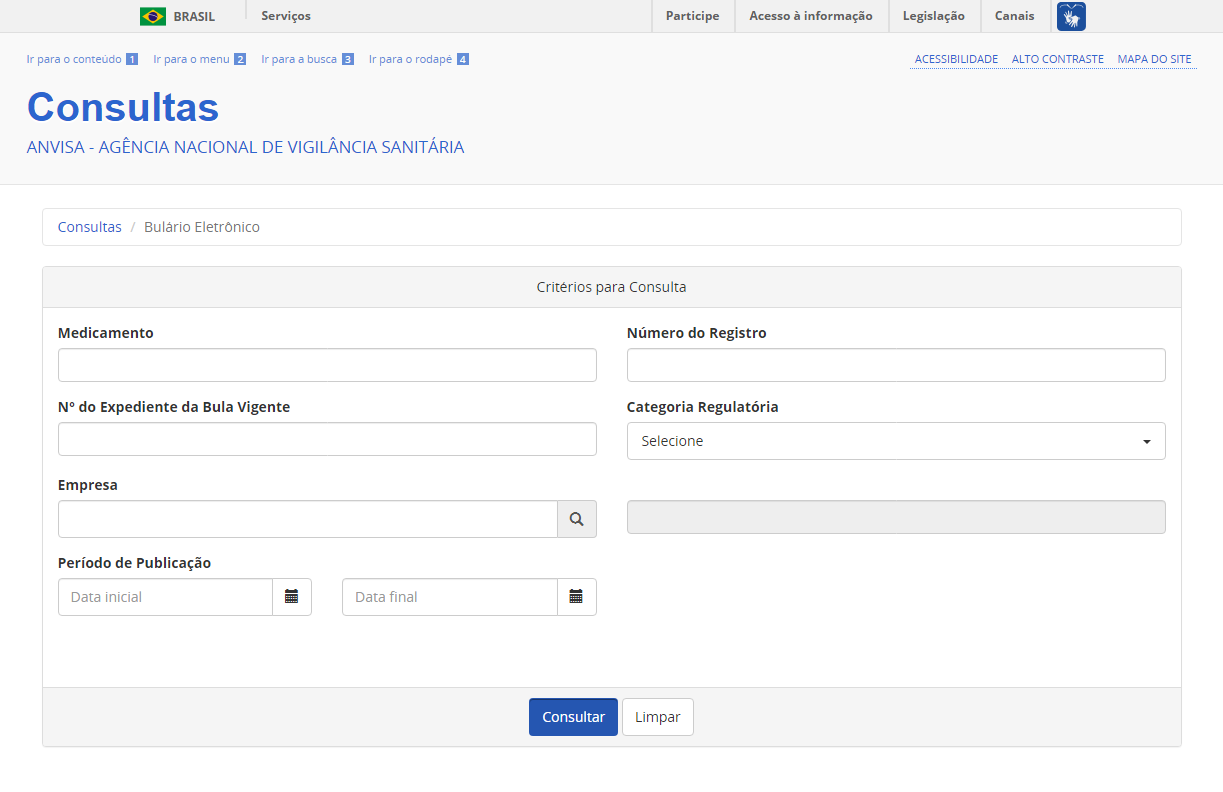
\includegraphics[width=\textwidth]{../pictures/bulario_pagina.png}
    \caption*{Fonte: \href{https://consultas.Anvisa.gov.br/\#/bulario/}{Portal da \ac{Anvisa}}, acesso em 2023-09-06.}
\end{figure}

Para exemplificar a busca, foi escolhido o medicamento TYSABRI\textsuperscript{\tiny\textregistered}.
O nome foi inserido no campo ``Medicamento'' e foi realizada a consulta.
A \autoref{fig:bulario_resultado} apresenta a interface da página com os resultados da busca, neste caso, há apenas um registro no banco de dados da \ac{Anvisa}.

\begin{figure}[!htbp]
    \centering
    \caption[Página de resultados de consulta ao Bulário Eletrônico da \acs{Anvisa}]{Página de resultados de consulta ao Bulário Eletrônico da \acs{Anvisa}, medicamento TYSABRI\textsuperscript{\tiny\textregistered}.}
    \label{fig:bulario_resultado}
    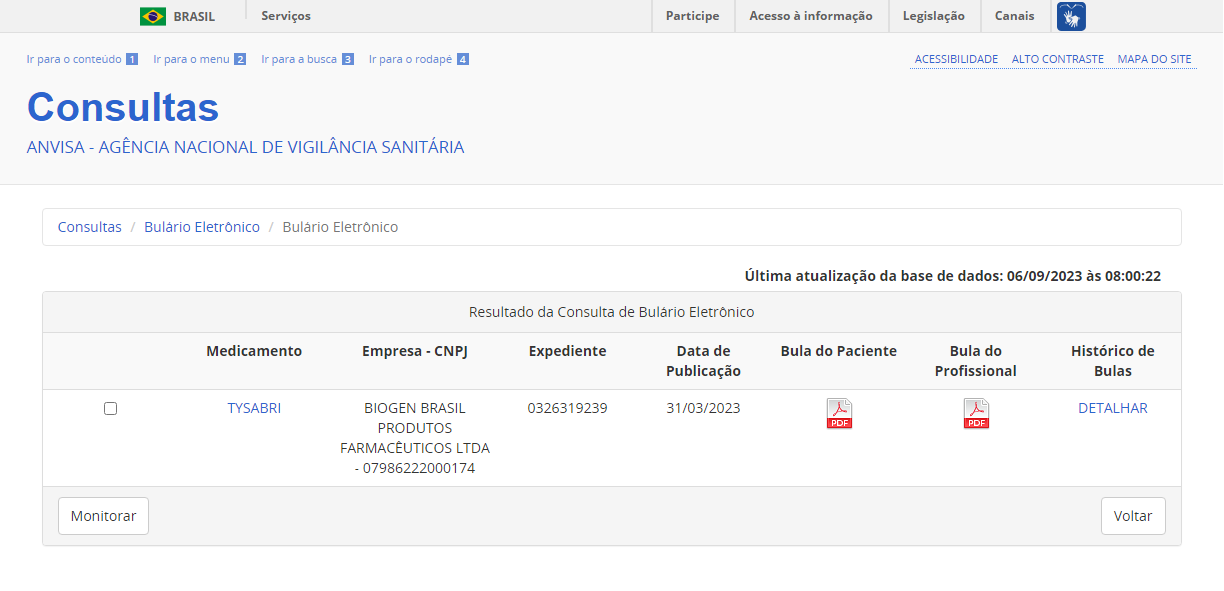
\includegraphics[width=\textwidth]{../pictures/bulario_resultado.png}
    \caption*{Fonte: \href{https://consultas.Anvisa.gov.br/\#/bulario/q/?nomeProduto=TYSABRI}{Portal da \ac{Anvisa}}, acesso em 2023-09-06.}
\end{figure}

Por fim, clicando no nome do medicamento na lista, foi acessada a página de detalhes, apresentada na \autoref{fig:bulario_detalhes}.

\begin{figure}[!htbp]
    \centering
    \caption[Página de detalhes do produto no Bulário Eletrônico da \acs{Anvisa}]{Página de detalhes do produto no Bulário Eletrônico da \acs{Anvisa}, medicamento TYSABRI\textsuperscript{\tiny\textregistered}.}
    \label{fig:bulario_detalhes}
    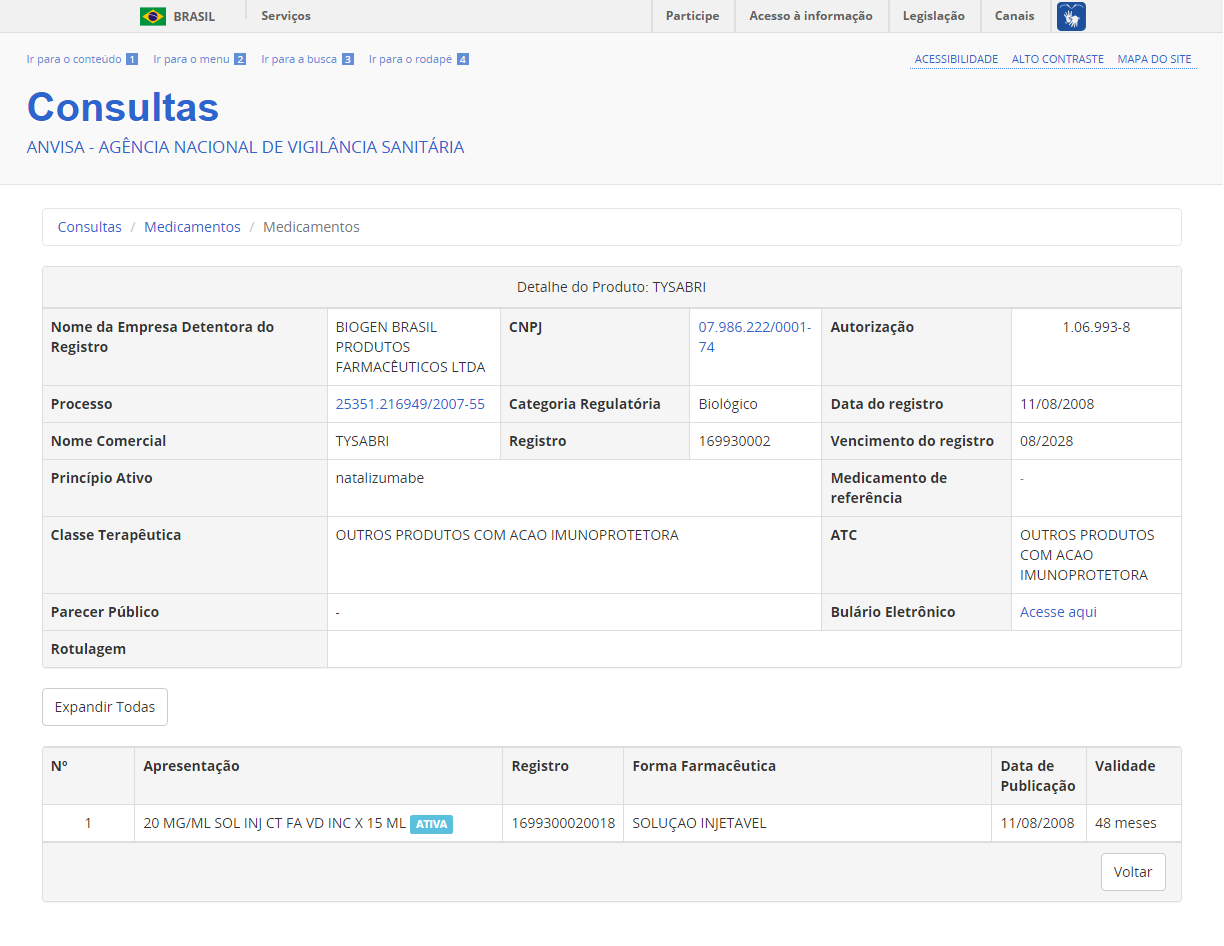
\includegraphics[width=\textwidth]{../pictures/bulario_detalhes.png}
    \caption*{Fonte: \href{https://consultas.Anvisa.gov.br/\#/medicamentos/25351216949200755/}{Portal da \ac{Anvisa}}, acesso em 2023-09-06.}
\end{figure}

Infelizmente o portal da \ac{Anvisa} não disponibiliza uma \ac{API} para acesso ao bulário, o que dificulta o uso deste por programadores e pesquisadores.
Com o objetivo de contornar este problema, \citeauthor{landin2022bulario} \cite{landin2022bulario} criou uma biblioteca em JavaScript que realiza a busca no sistema da \ac{Anvisa} e retorna um objeto JSON com os resultados da busca.

Ainda para ampliar a portabilidade da biblioteca, \citeauthor{landin2022api} também desenvolveu uma \ac{API} para a realização das buscas utilizando requisições web GET \cite{landin2022api}.
O \autoref{cod:sh} apresenta um exemplo de requisição GET para a busca de um medicamento usando o Bulario \ac{API}, e o \autoref{cod:json} apresenta o JSON retornado pela requisição.

\begin{lstfloat}[p]
    \centering
    \lstinputlisting[language=sh, label=cod:sh,
    caption={Exemplo de código de requisição para o medicamento TYSABRI\textsuperscript{\tiny\textregistered} no Bulário \ac{API}.}
    ]{../code/bulario_api.sh}
    \caption*{Fonte: \href{https://bula.vercel.app/docs}{Documentação Bulario \ac{API}}, acesso em 2023-09-06, adaptado.}
\end{lstfloat}

\begin{lstfloat}[p]
    \centering
    \lstinputlisting[language=JavaScript, label=cod:json, caption={Arquivo JSON retornado pela busca ao medicamento TYSABRI\textsuperscript{\tiny\textregistered} no Bulário \ac{API}}]{../code/tysabri.json}
    \caption*{Fonte: \href{https://bula.vercel.app/docs}{Documentação Bulario \ac{API}}, acesso em 2023-09-06, adaptado.}
\end{lstfloat}

% \cite{landin2022api, landin2022bulario, Anvisa2020bulario, Anvisa2009RDC}

\section{Trabalhos Relacionados}

A proposta aqui apresentada já foi explorada anteriormente em outros trabalhos.
Esta seção cita alguns destes, descrevendo propostas, metodologias e dificuldades.

O trabalho apresentado por \citeauthor{steffenon2020katie} \cite{steffenon2020katie} consiste em uma aplicação \textit{mobile}, KATIE, que auxilia pessoas com baixa ou nenhuma visão na realização de tarefas simples.
Esta aplicação tem como objetivo o reconhecer, interpretar e responder perguntas feitas pelo usuário sobre seu ambiente, em alguns casos, com o auxílio da câmera do dispositivo.
A interface com o usuário foi feita baseada em métodos de reconhecimento de fala, bem como conversão da resposta obtida pelo sistema em áudio.
O desenvolvimento teve como enfoque o público alvo, visando ser uma tecnologia assistiva eficiente.
Seus resultados atenderam as expectativas da proposta, conseguindo identificar cédulas de dinheiro e rótulos de medicamentos.

\citeauthor{gadenz2019desenvolvimento} \cite{gadenz2019desenvolvimento} faz uma proposta semelhante a anterior, porém com o enfoque em pessoas acima de 60 anos, tendo em vista que nesta idade, baixas de visão são mais comuns.
A aplicação proposta, além de identificar o medicamento pelo rótulo, também é capaz de fornecer sua bula.
Outra preocupação desse trabalho é relacionada ao risco de efeitos adversos que esses medicamentos podem causar por uso indevido.
Os testes realizados com processamento local, foi obtida uma taxa de acerto de \SI{100}{\percent} para os seis medicamentos cadastrados.

Em sua tese, \citeauthor{benjamim2012identificaccao} \cite{benjamim2012identificaccao} sugere o uso de um sistema para auxiliar a identificação de caixas de medicamentos para pessoas com deficiência visual, com o objetivo de evitar ingestão errônea desses remédios.
A proposta também almeja auxiliar o usuário com detalhes quanto à posologia do medicamento, bem como indicações e contra indicações.
Essa proposta sugere o uso de dispositivos diversos que estariam inseridos do dia a dia dos usuários, desde celulares até televisores.

\citeauthor{rodrigues2022sisamed} \cite{rodrigues2022sisamed} aponta problemas com não adesão ou adesão parcial de pacientes ao uso dos medicamentos, e propõe um sistema capaz de reconhecer automaticamente estes remédios, além de lembrar o paciente nos horários que estes dever ser tomados.
Esta proposta se baseia no uso de um microcomputador, acoplado a uma \textit{webcam} apontada para a superfície onde os medicamentos seriam reservados.
O sistema alertará o paciente no horário correto para que o remédio seja tomado, interrompendo o alerta somente quando detectar que houve interação com o medicamento sobre a mesa.



    \chapter{Metodologia}\label{cap:metodologia}

% \MexerDepois{Escrever algo aqui}

Neste capítulo, são explorados os métodos utilizados para a construção do trabalho proposto, inicialmente com uma apresentação geral e em seguida com uma apresentação detalhada.

\section{Abordagem}

A abordagem utilizada no sistema consiste em, inicialmente, carregar o arquivo de imagem correspondente à foto do remédio a ser buscado.
Dessa imagem, são geradas versões em diferentes codificações de cores, e cada uma tem suas componentes analisadas.

A análise de cada versão resulta numa lista de termos textuais, que serão organizados e buscados no sistema do Bulário Eletrônico da \ac{Anvisa} \cite{anvisa2020bulario}.

Se um dos termos buscado for encontrado com sucesso, será carregado o arquivo digital da bula deste medicamento.
A \autoref{fig:fluxograma} apresenta o fluxograma geral do funcionamento do sistema.

\begin{figure}[htbp]
    \centering
    % 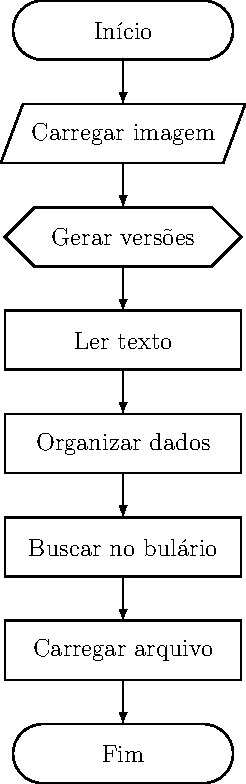
\includegraphics{../pictures/fluxograma_0.pdf}
    \caption{Fluxograma geral do funcionamento.}
    % https://www.youtube.com/watch?v=e968B1PwIbs&list=PLkRY1UknxTS0exb3ccUBJS1_e0TlSozFW&index=2

\begin{tikzpicture}[node distance=1.5cm]
    \node (s) [startstop] {Início};
    \node (a1) [below of=s, io] {Carregar imagem};
    \node (a2) [below of=a1, process] {Gerar versão};
    \node (a3) [below of=a2, process] {Ler texto};
    \node (a4) [below of=a3, loop] {Há outra versão?};
    \node (a5) [below of=a4, process] {Organizar dados};
    \node (a6) [below of=a5, process] {Buscar no bulário};
    \node (a7) [below of=a6, process] {Carregar arquivo};
    \node (f)  [below of=a7, startstop] {Fim};

    \node [left of=a1, auxBlockPhantom] {\phantom{\autoref{ssec:carregar}}};

    \node [right of=a1, auxBlock] {\autoref{ssec:carregar}};
    \node [right of=a2, auxBlock] {\autoref{ssec:versoes}};
    \node [right of=a3, auxBlock] {\autoref{ssec:ler}};
    \node [right of=a5, auxBlock] {\autoref{ssec:organizar}};
    \node [right of=a6, auxBlock] {\autoref{ssec:buscar}};
    \node [right of=a7, auxBlock] {\autoref{ssec:arquivo}};

    \draw [niceBrace] ([yshift=0.6cm, xshift=2.25cm]a1.center) -- ([yshift=-0.6cm, xshift=2.25cm]a1.center);
    \draw [niceBrace] ([yshift=0.6cm, xshift=2.25cm]a2.center) -- ([yshift=-0.6cm, xshift=2.25cm]a2.center);
    \draw [niceBrace] ([yshift=0.6cm, xshift=2.25cm]a3.center) -- ([yshift=-0.6cm, xshift=2.25cm]a3.center);
    \draw [niceBrace] ([yshift=0.6cm, xshift=2.25cm]a5.center) -- ([yshift=-0.6cm, xshift=2.25cm]a5.center);
    \draw [niceBrace] ([yshift=0.6cm, xshift=2.25cm]a6.center) -- ([yshift=-0.6cm, xshift=2.25cm]a6.center);
    \draw [niceBrace] ([yshift=0.6cm, xshift=2.25cm]a7.center) -- ([yshift=-0.6cm, xshift=2.25cm]a7.center);

    \node [anchor=north west, font = {\scriptsize\bfseries}, Red] at (a4.south) {N};
    \node [anchor=south east, font = {\scriptsize\bfseries}, Green] at (a4.west) {S};

    % \node [fit=(a1)] (fita1) {}; \draw [niceBrace] ([yshift=2.5pt]fita1.north east) -- ([yshift=-2.5pt]fita1.south east);
    % \node [fit=(a2)] (fita2) {}; \draw [niceBrace] ([yshift=2.5pt]fita2.north east) -- ([yshift=-2.5pt]fita2.south east);
    % \node [fit=(a3)] (fita3) {}; \draw [niceBrace] ([yshift=2.5pt]fita3.north east) -- ([yshift=-2.5pt]fita3.south east);
    % \node [fit=(a5)] (fita5) {}; \draw [niceBrace] ([yshift=2.5pt]fita5.north east) -- ([yshift=-2.5pt]fita5.south east);
    % \node [fit=(a6)] (fita6) {}; \draw [niceBrace] ([yshift=2.5pt]fita6.north east) -- ([yshift=-2.5pt]fita6.south east);
    % \node [fit=(a7)] (fita7) {}; \draw [niceBrace] ([yshift=2.5pt]fita7.north east) -- ([yshift=-2.5pt]fita7.south east);


    \draw [arrow] (s) -- (a1);
    \draw [arrow] (a1) -- (a2);
    \draw [arrow] (a2) -- (a3);
    \draw [arrow] (a3) -- (a4);
    \draw [arrow] (a4) -- (a5);
    \draw [arrow] (a4) -- ([xshift=-.5cm]a4.west) |- (a2);
    \draw [arrow] (a5) -- (a6);
    \draw [arrow] (a6) -- (a7);
    \draw [arrow] (a7) -- (f);
\end{tikzpicture}
% \begin{tikzpicture}[node distance=1.5cm]
%     \node (s) [startstop] {Início};
%     \node (a1) [below of=s, io] {Carregar imagem};
%     \node (a2) [below of=a1, loop] {Gerar versões};
%     \node (a3) [right of=a1, node distance=5cm, process] {Ler texto};
%     \node (a5) [below of=a3, process] {Organizar dados};
%     \node (a6) [right of=a3, node distance=5cm, process] {Buscar no bulário};
%     \node (a7) [below of=a6, process] {Carregar arquivo};
%     \node (f)  [below of=a7, startstop] {Fim};

%     \draw [arrow] (s) -- (a1);
%     \draw [arrow] (a1) -- (a2);
%     \draw [arrow] (a2) -| ($(a2)!0.5!(a3)$) |- (a3);
%     \draw [arrow] (a3) -- (a5);
%     \draw [arrow] (a5) -| ($(a5)!0.5!(a6)$) |- (a6);
%     \draw [arrow] (a6) -- (a7);
%     \draw [arrow] (a7) -- (f);
% \end{tikzpicture}
% \begin{tikzpicture}[node distance=1.5cm]
%     \node (s) [startstop] {Início};
%     \node (a1) [below of=s, io] {Carregar imagem};
%     \node (a2) [right of=a1, node distance=5cm, loop] {Gerar versões};
%     \node (a3) [right of=a2, node distance=5cm, process] {Ler texto};
%     \node (a5) [below of=a1, node distance=2cm, process] {Organizar dados};
%     \node (a6) [right of=a5, node distance=5cm, process] {Buscar no bulário};
%     \node (a7) [right of=a6, node distance=5cm, process] {Carregar arquivo};
%     \node (f)  [below of=a7, startstop] {Fim};

%     \draw [arrow] (s) -- (a1);
%     \draw [arrow] (a1) -- (a2);
%     \draw [arrow] (a2) -- (a3);
%     \draw [arrow] (a3) |- ($(a3)!0.5!(a5)$) -| (a5);
%     \draw [arrow] (a5) -- (a6);
%     \draw [arrow] (a6) -- (a7);
%     \draw [arrow] (a7) -- (f);
% \end{tikzpicture}
    \caption*{Fonte: Autor.}
    \label{fig:fluxograma}
\end{figure}

\section{Detalhamento}

Nesta seção, serão detalhados os métodos utilizados em cada passo da análise da imagem.

\subsection{Carregar arquivo de imagem}\label{ssec:carregar}

O primeiro passo no processo de análise consiste em carregar a imagem do arquivo escolhido, para isso, foi utilizada a função \textit{imread}, da biblioteca de processamento de imagem \textit{OpenCV}.

Essa função retorna os dados da imagem como um tensor no formato \acs{BGR} \cite{CV2imread}.
Em seguida, a imagem é convertida para o formato \ac{RGB} e é dado início ao processo de leitura do texto na imagem.

O \autoref{cod:carregar} apresenta a simplificação do bloco de código responsável por realizar essa ação.

\begin{lstfloat}[htbp]
    \centering
    \lstinputlisting[label=cod:carregar, caption={Carregar arquivo de imagem, simplificado.}]{../code/ex_carregar.py}
    \caption*{Fonte: Autor.}
\end{lstfloat}

\subsection{Realizar leitura do texto na imagem}\label{ssec:ler}

O processamento do texto presente na imagem é realizado através do motor de \ac{OCR} \textit{Tesseract OCR}, sendo interfaceado pela função \textit{image\_to\_data} da biblioteca \textit{pytesseract}, desenvolvida para facilitar o uso deste motor em Python \cite{samuelhoffstaetter2024, tesseract2024}.
O \autoref{cod:ler} apresenta uma simplificação da primeira parte do bloco de código associado a leitura dos termos.

\begin{lstfloat}[htbp]
    \centering
    \lstinputlisting[label=cod:ler, caption={Ler texto da imagem, simplificado.}]{../code/ex_ler.py}
    \caption*{Fonte: Autor.}
\end{lstfloat}


Essa função retorna a lista de termos encontrados, junto de informações adicionais a respeito, como confiabilidade e coordenadas da caixa que envolve o termo na imagem \cite{samuelhoffstaetter2024}.
As informações adicionais são utilizadas para filtrar e posteriormente classificar a ordem de prioridade da análise dos termos encontrados.

A filtragem realizada nesta etapa consiste em descartar termos com confiabilidade abaixo de \SI{10}{\percent} ou área menor que um parâmetro padrão.
A área mínima é relativa ao tamanho da imagem, em quantidade de \acp{pixel}, dado pela \autoref{eq:area_minima}, calculado pelo piso dos produtos de \SI{2}{\percent} das dimensões totais da imagem.
A \autoref{fig:fotos:tamanho} apresenta um exemplo da área mínima que um termo deve ocupar para ser considerado.
O \autoref{cod:ler:2} apresenta a continuação da lógica simplificada envolvida nessa seção.

\begin{equation}\label{eq:area_minima}
    A_\text{termo} \geq \left\lfloor\frac{w_\text{img}\cdot h_\text{img}}{2500}\right\rfloor = \left\lfloor \left(w_\text{img} \cdot \SI{2}{\percent}\right) \cdot \left(h_\text{img} \cdot \SI{2}{\percent}\right) \right\rfloor
\end{equation}

\begin{figure}[htb]
    \centering
    \caption{Exemplo de foto do medicamento TYSABRI\textsuperscript{\tiny\textregistered}, com destaque em vermelho da área mínima para um termo ser considerado. Imagem completa (\subref{fig:fotos:tysabri}) e com recorte próximo ao termo (\subref{fig:fotos:tysabri_cortado}).}
    \hfill
    \begin{subfigure}[t]{0.45\textwidth}
        \centering
        \caption{Imagem completa com destaque de área.}
        \label{fig:fotos:tysabri}
        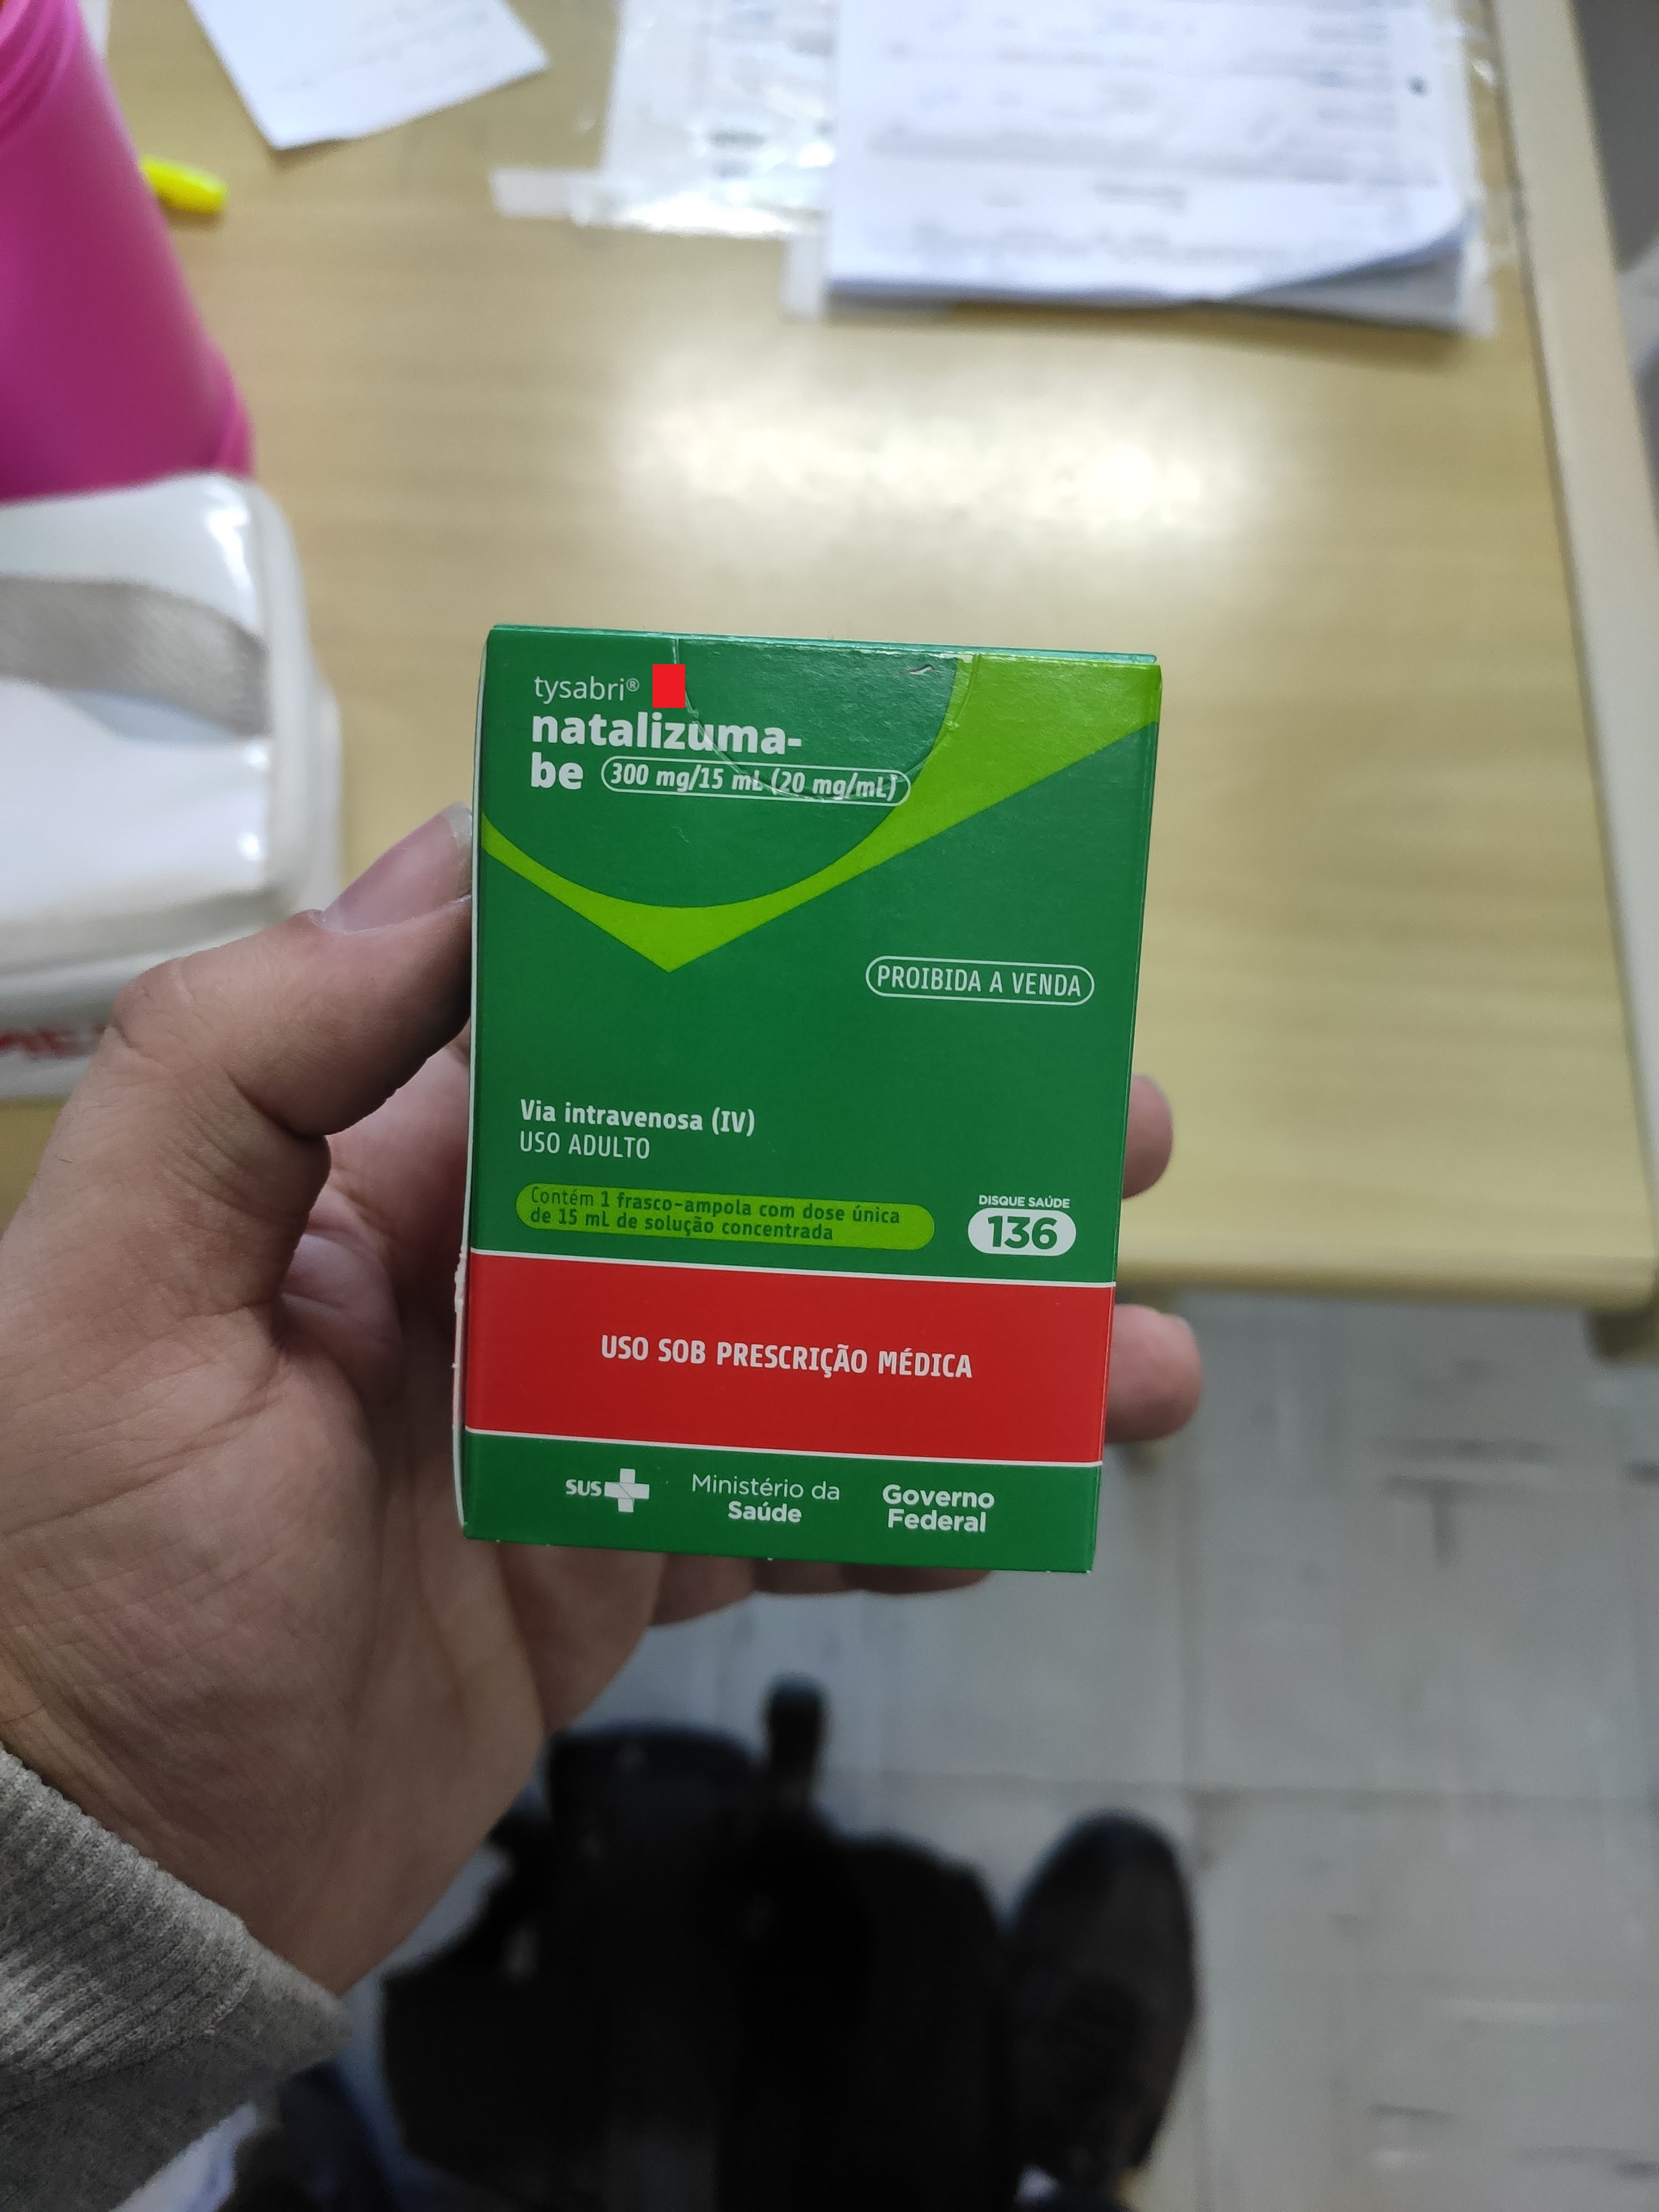
\includegraphics[width=\linewidth]{../pictures/tysabri.jpg}
        \caption*{Fonte: Autor.}
    \end{subfigure}
    \hfill
    \begin{subfigure}[t]{0.45\textwidth}
        \centering
        \caption{Recorte ao redor da área destacada.}
        \label{fig:fotos:tysabri_cortado}
        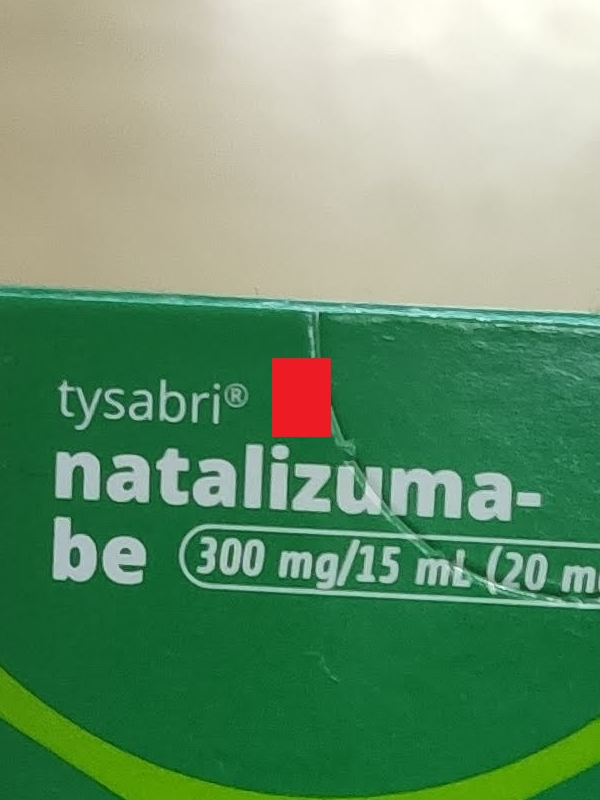
\includegraphics[width=\linewidth]{../pictures/tysabri cortado.jpg}
        \caption*{Fonte: Autor.}
    \end{subfigure}
    \hfill
    \label{fig:fotos:tamanho}
\end{figure}


\begin{lstfloat}[htbp]
    \centering
    \lstinputlisting[label=cod:ler:2, caption={Filtrar termos lidos, simplificado.}]{../code/ex_ler_2.py}
    \caption*{Fonte: Autor.}
\end{lstfloat}

\subsection{Gerar diferentes versões de imagem}\label{ssec:versoes}

Além da análise realizada na versão codificada em \ac{RGB} da imagem, também são analisadas variantes em codificação de cores nessa imagem, além da versão em escala de cinza.
Para cada codificação, são analisadas suas componentes separadamente.
Caso duas componentes encontrem palavras iguais, é mantida na lista a versão com maior valor de confiabilidade.
As diversas componentes das codificações analisadas viabilizam a localização de novos termos, já que cada uma trará um novo perfil de contraste à imagem.

Em cada componente analisada, é aplicado um método de limiar para binarização dos valores.
As componentes binarizadas são utilizadas para recompor a imagem completa da codificação em questão e essa nova versão também é analisada.

As codificações analisadas foram:
\begin{itemize}
    \item \ac{RGB};
    \item \ac{CMYK};
    \item HLS;
    \item HSV;
    \item YCrCb.
\end{itemize}

A conversão para as versões HLS, HSV e YCrCb foi realizada através da função \lstinline|cvtColor|, da biblioteca de processamento de imagem \textit{OpenCV}, essa função converte a codificação de cores utilizada na imagem \cite{CV2cvtColor}.
A versão \ac{CMYK} é convertida utilizando as equações pertinentes.
A \autoref{fig:foto:codf} ilustra as demais codificações utilizadas.

\begin{figure}[htb]
    \centering
    \caption{Exemplo de foto do medicamento TYSABRI\textsuperscript{\tiny\textregistered} em diferentes codificações de cores.}
    \begin{subfigure}[t]{0.22\textwidth}
        \centering
        \caption{CMYK.}
        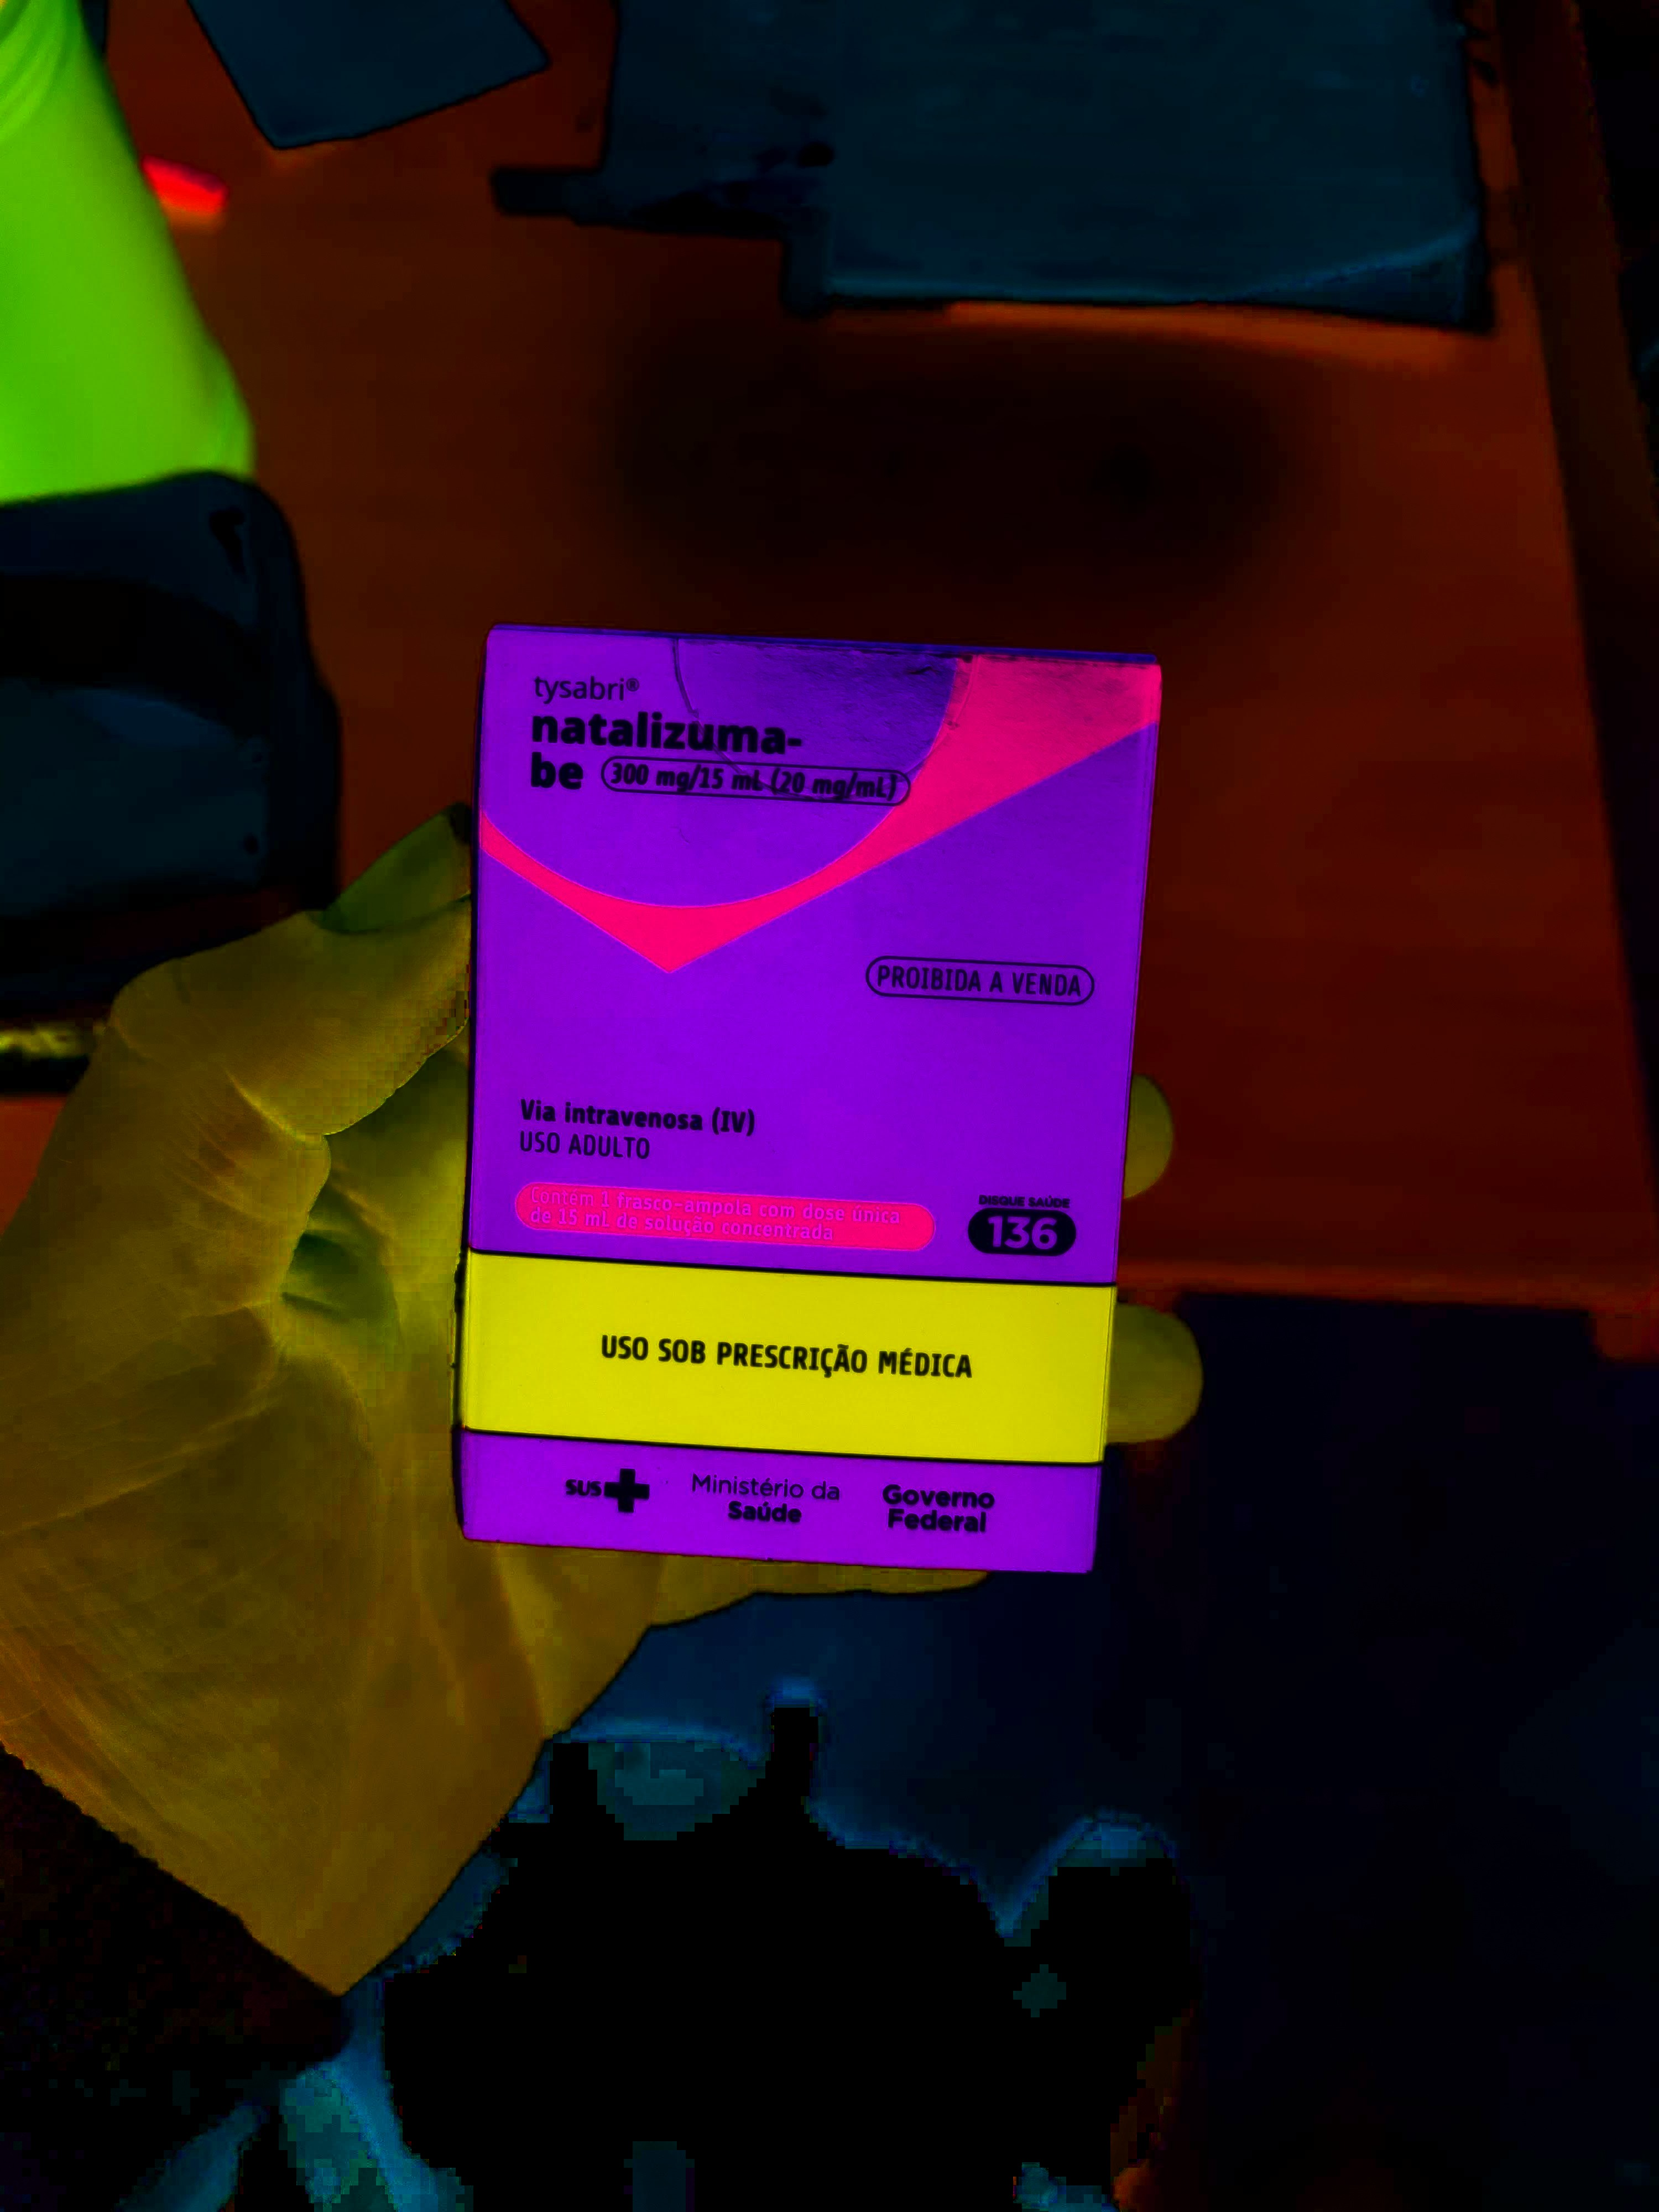
\includegraphics[width=\linewidth]{../pictures/tysabri_cmyk.jpg}
    \end{subfigure}
    \hfill
    \begin{subfigure}[t]{0.22\textwidth}
        \centering
        \caption{HLS.}
        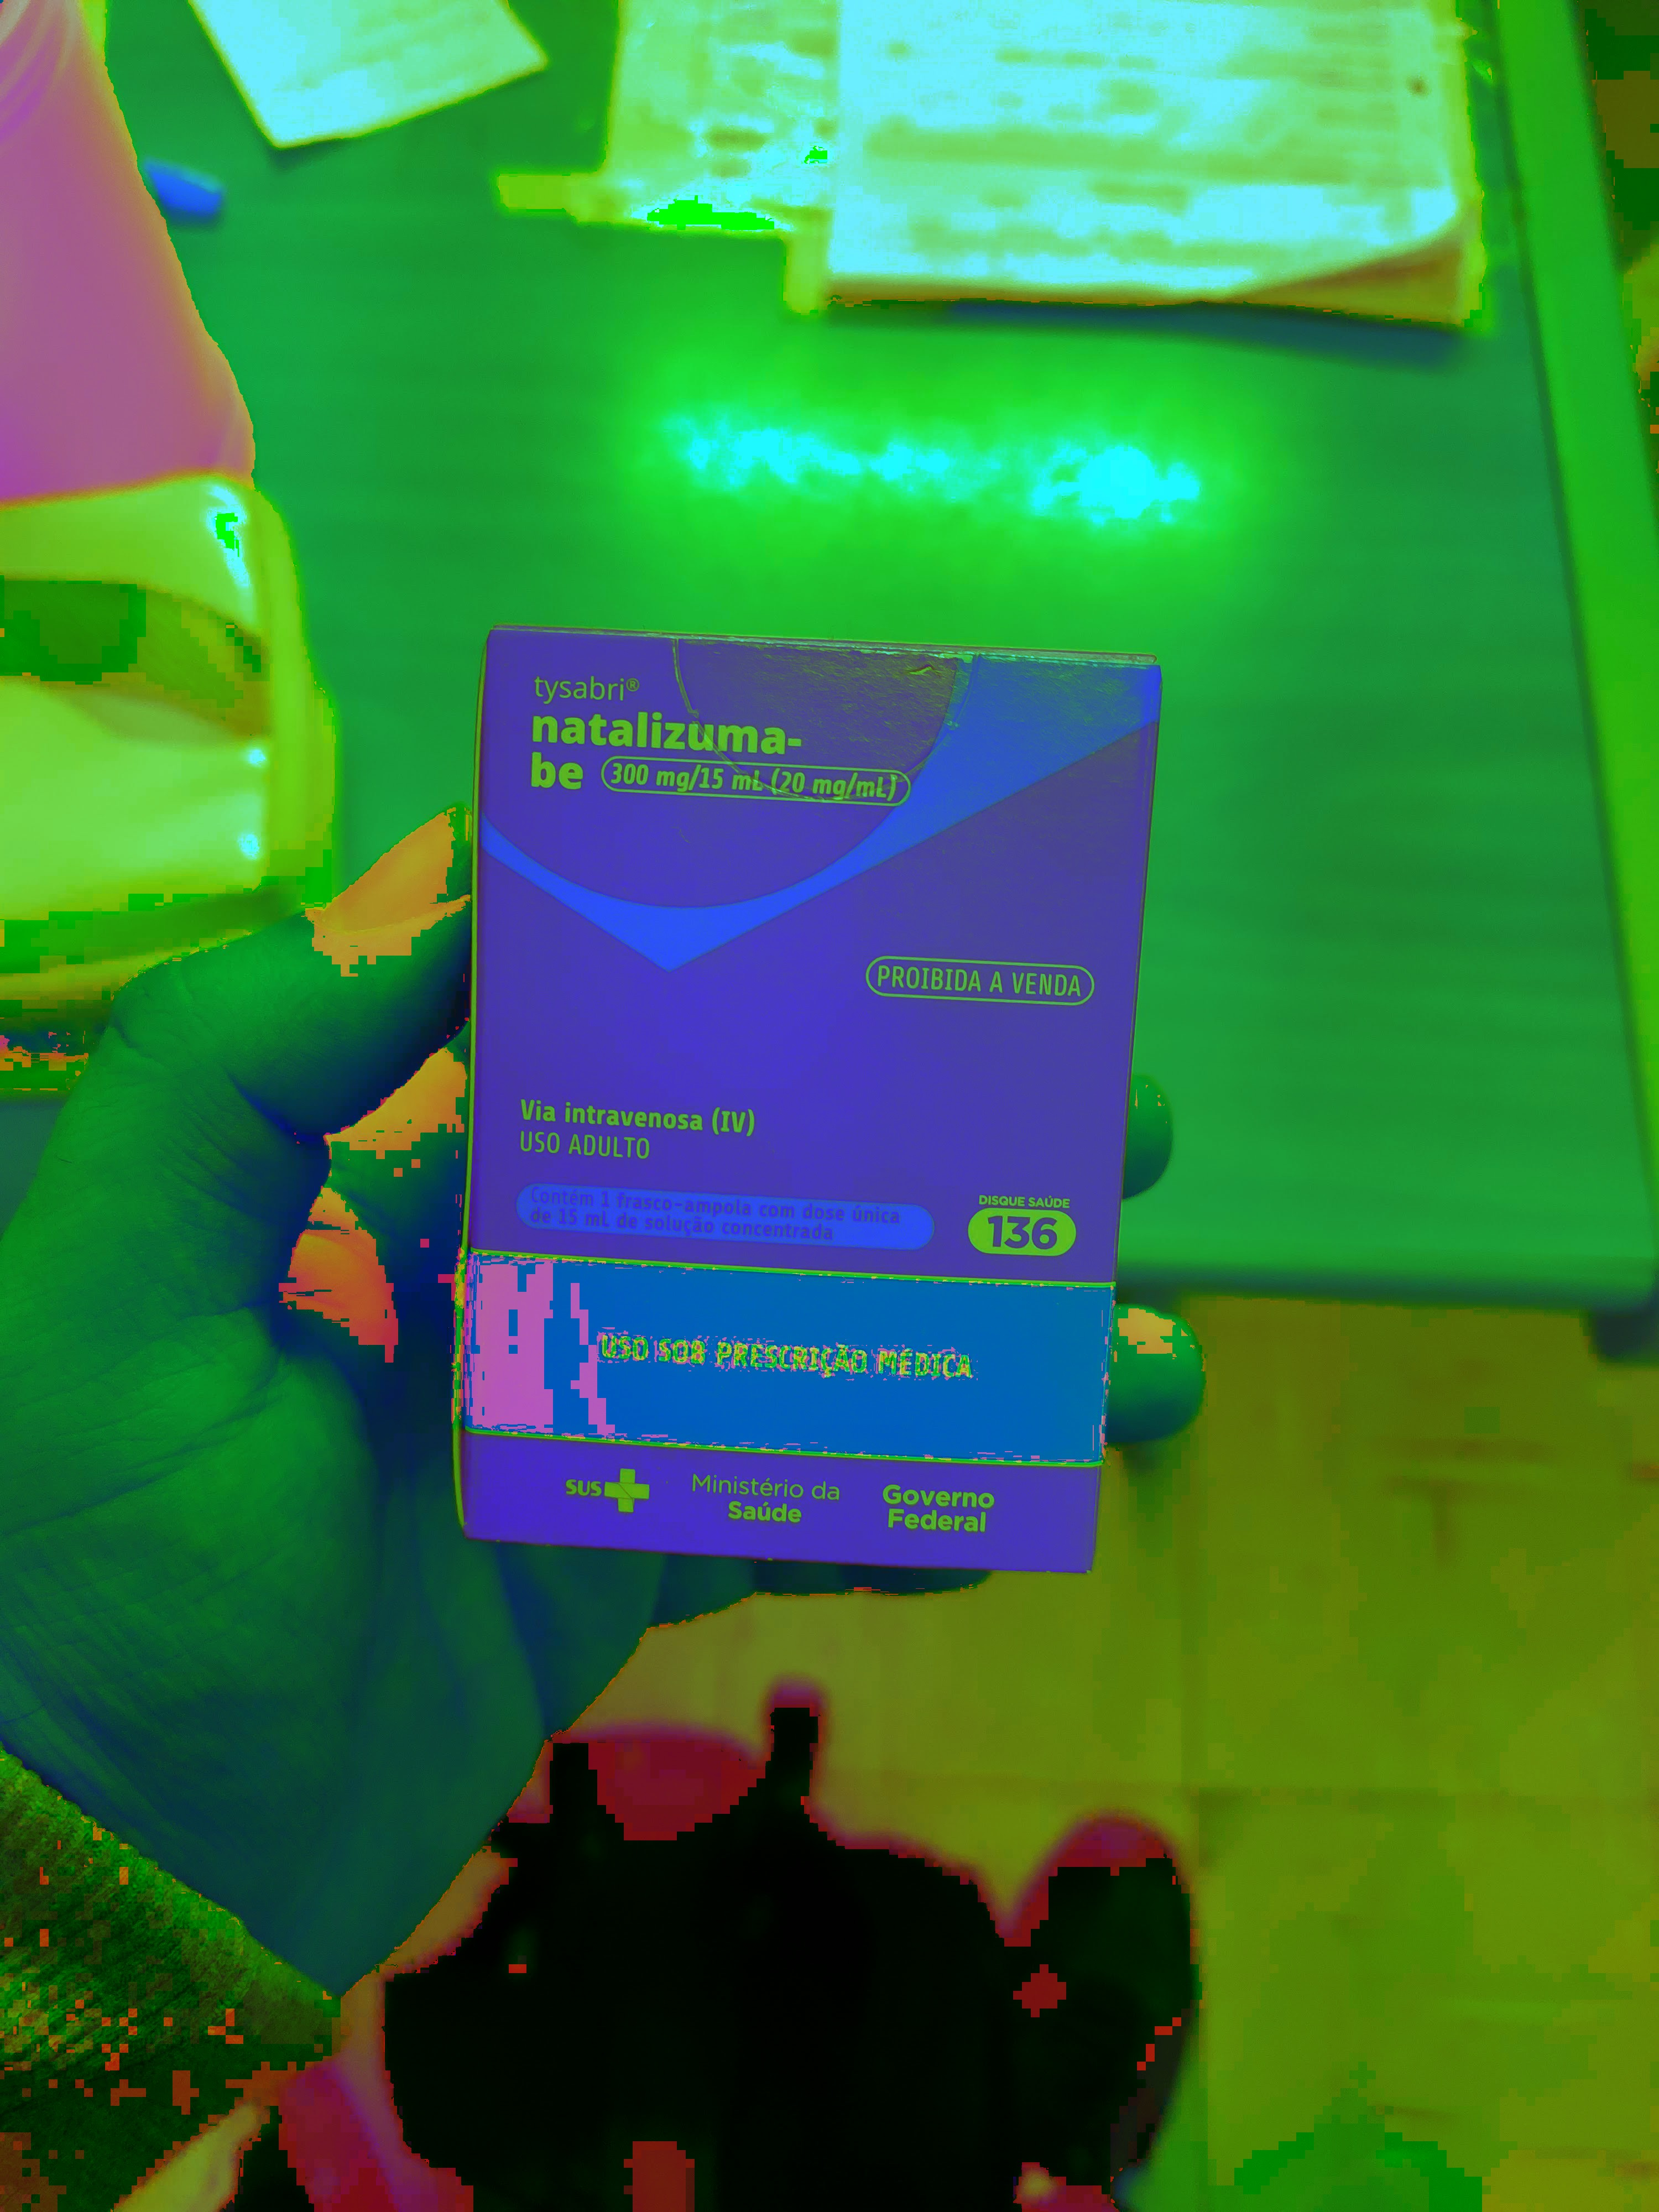
\includegraphics[width=\linewidth]{../pictures/tysabri_HLS.jpg}
    \end{subfigure}
    \hfill
    \begin{subfigure}[t]{0.22\textwidth}
        \centering
        \caption{HSV.}
        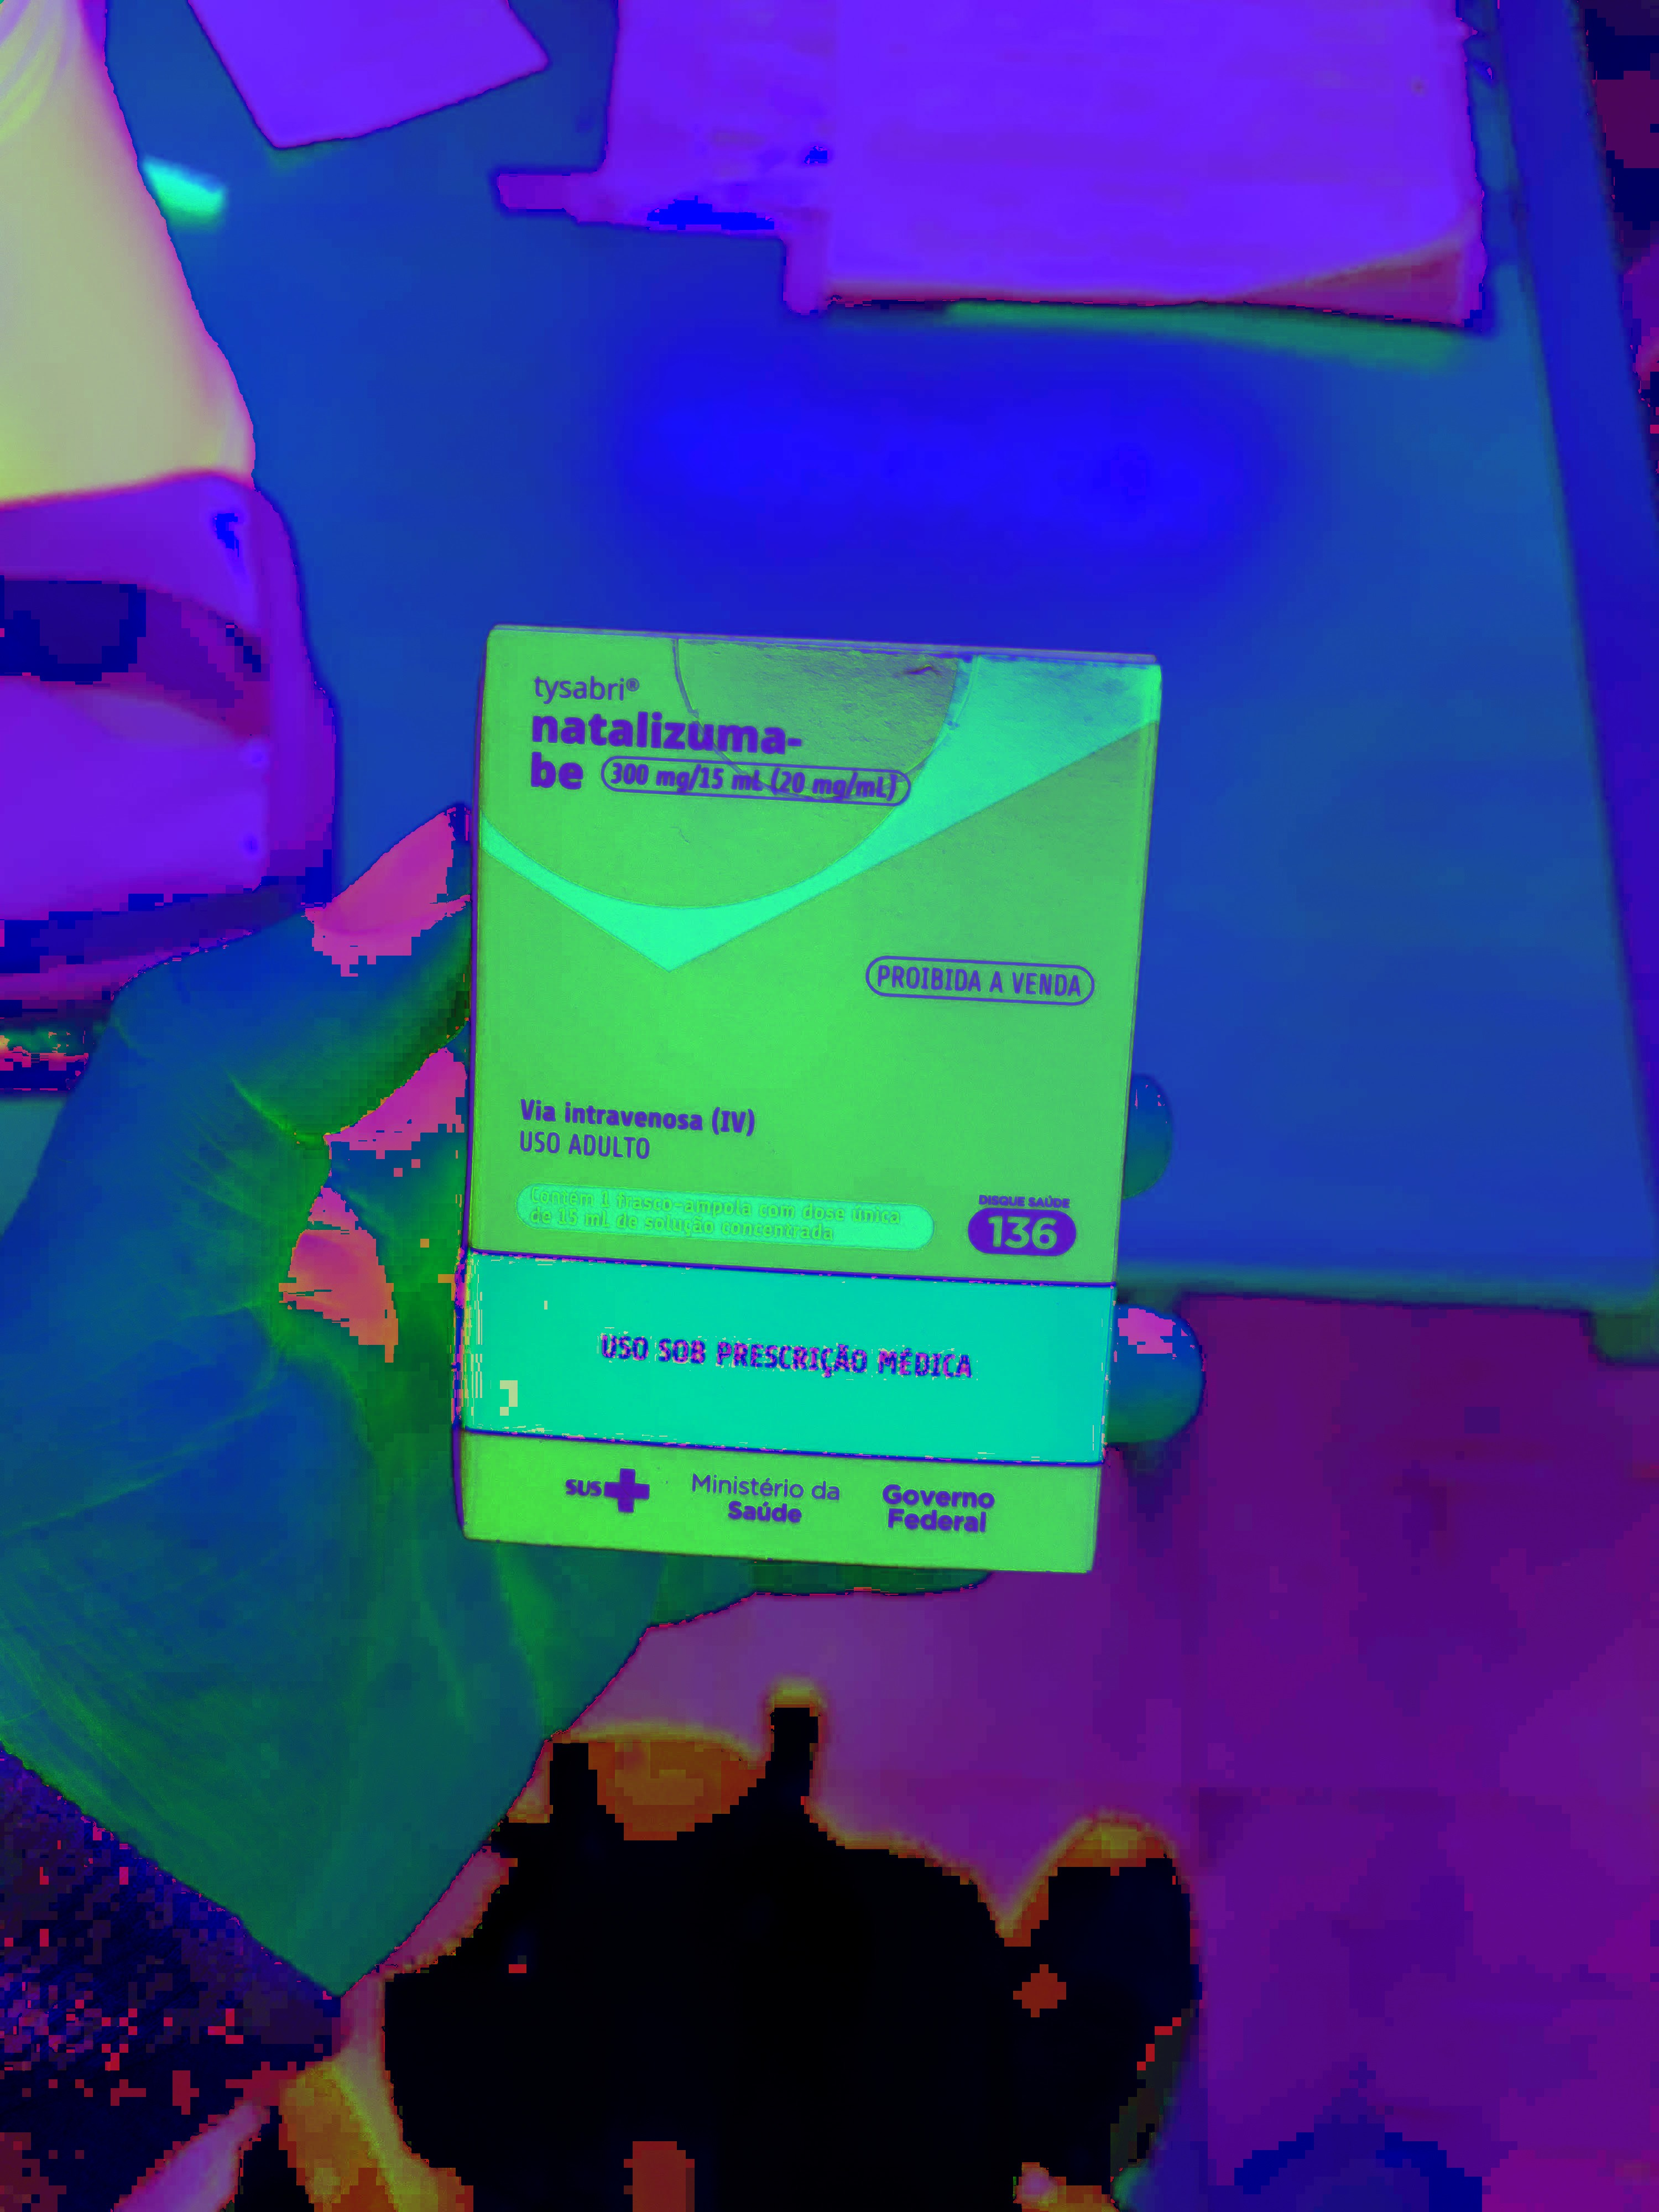
\includegraphics[width=\linewidth]{../pictures/tysabri_HSV.jpg}
    \end{subfigure}
    \hfill
    \begin{subfigure}[t]{0.22\textwidth}
        \centering
        \caption{YCrCb.}
        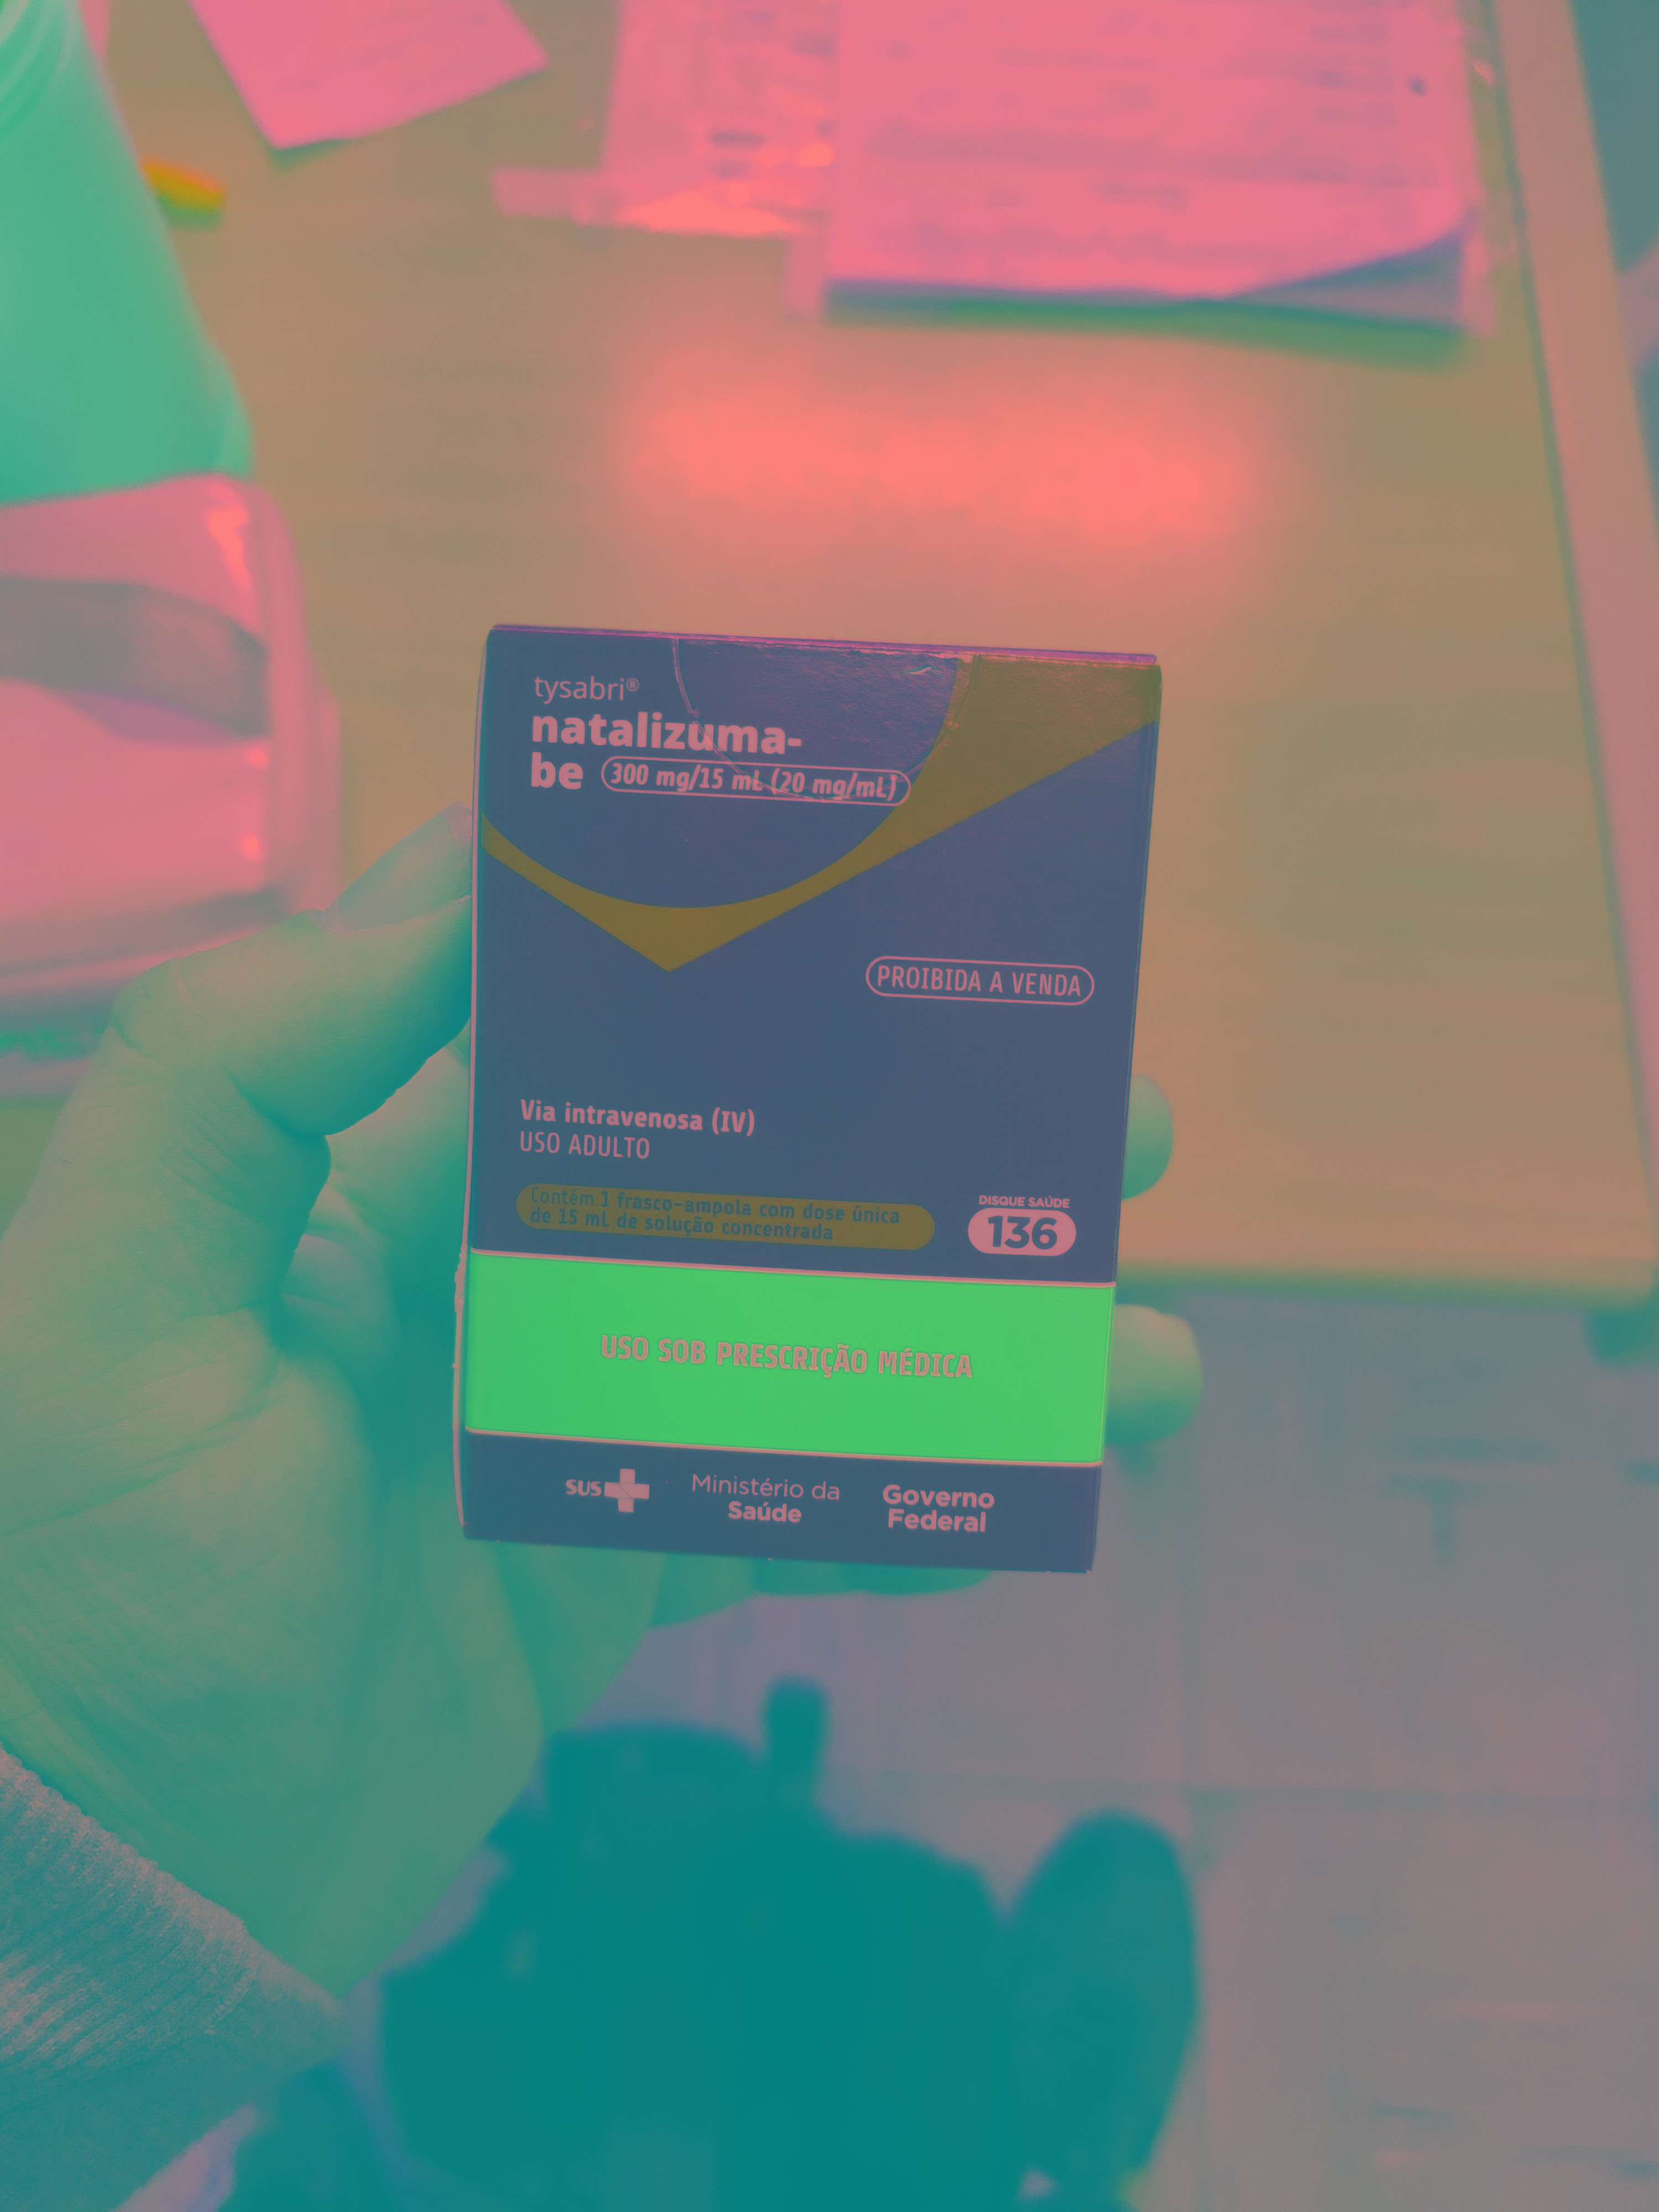
\includegraphics[width=\linewidth]{../pictures/tysabri_YCrCb.jpg}
    \end{subfigure}
    \caption*{Fonte: Autor.}
    \label{fig:foto:codf}
\end{figure}

A binarização por limiar das componentes é realizada pela função \textit{threshold}, da biblioteca de processamento de imagem \textit{OpenCV}, utilizando o método de Otsu \cite{CV2threshold}.
O \autoref{cod:versoes} apresenta uma simplificação da estrutura utilizada.
As Figuras \ref{fig:foto:versoes:1}, \ref{fig:foto:versoes:2} e \ref{fig:foto:versoes:3} apresentam exemplos de componentes analisadas, destacando os termos encontrados em cada uma.


\begin{lstfloat}[htbp]
    \centering
    \lstinputlisting[label=cod:versoes, caption={Gerar versões das imagens, simplificado.}]{../code/ex_versoes.py}
    \caption*{Fonte: Autor.}
\end{lstfloat}

\begin{figure}[htb]
    \centering
    \caption{Exemplos de componentes analisadas cinza e RGB (%
    \subref{fig:foto:versoes:1:Cinza},
    \subref{fig:foto:versoes:1:R},
    \subref{fig:foto:versoes:1:G},
    \subref{fig:foto:versoes:1:B},
    \subref{fig:foto:versoes:1:Cinza_thresh},
    \subref{fig:foto:versoes:1:R_thresh},
    \subref{fig:foto:versoes:1:G_thresh},
    \subref{fig:foto:versoes:1:B_thresh}%
    ) e destaque nos termos localizados em cada componente (%
    \subref{fig:foto:versoes:1:Cinza:boxes},
    \subref{fig:foto:versoes:1:R:boxes},
    \subref{fig:foto:versoes:1:G:boxes},
    \subref{fig:foto:versoes:1:B:boxes},
    \subref{fig:foto:versoes:1:Cinza_thresh:boxes},
    \subref{fig:foto:versoes:1:R_thresh:boxes},
    \subref{fig:foto:versoes:1:G_thresh:boxes},
    \subref{fig:foto:versoes:1:B_thresh:boxes}%
    ).}
    % \hfill
    \begin{subfigure}[t]{0.21\textwidth}
        \centering
        \caption{Cinza.}
        \label{fig:foto:versoes:1:Cinza}
        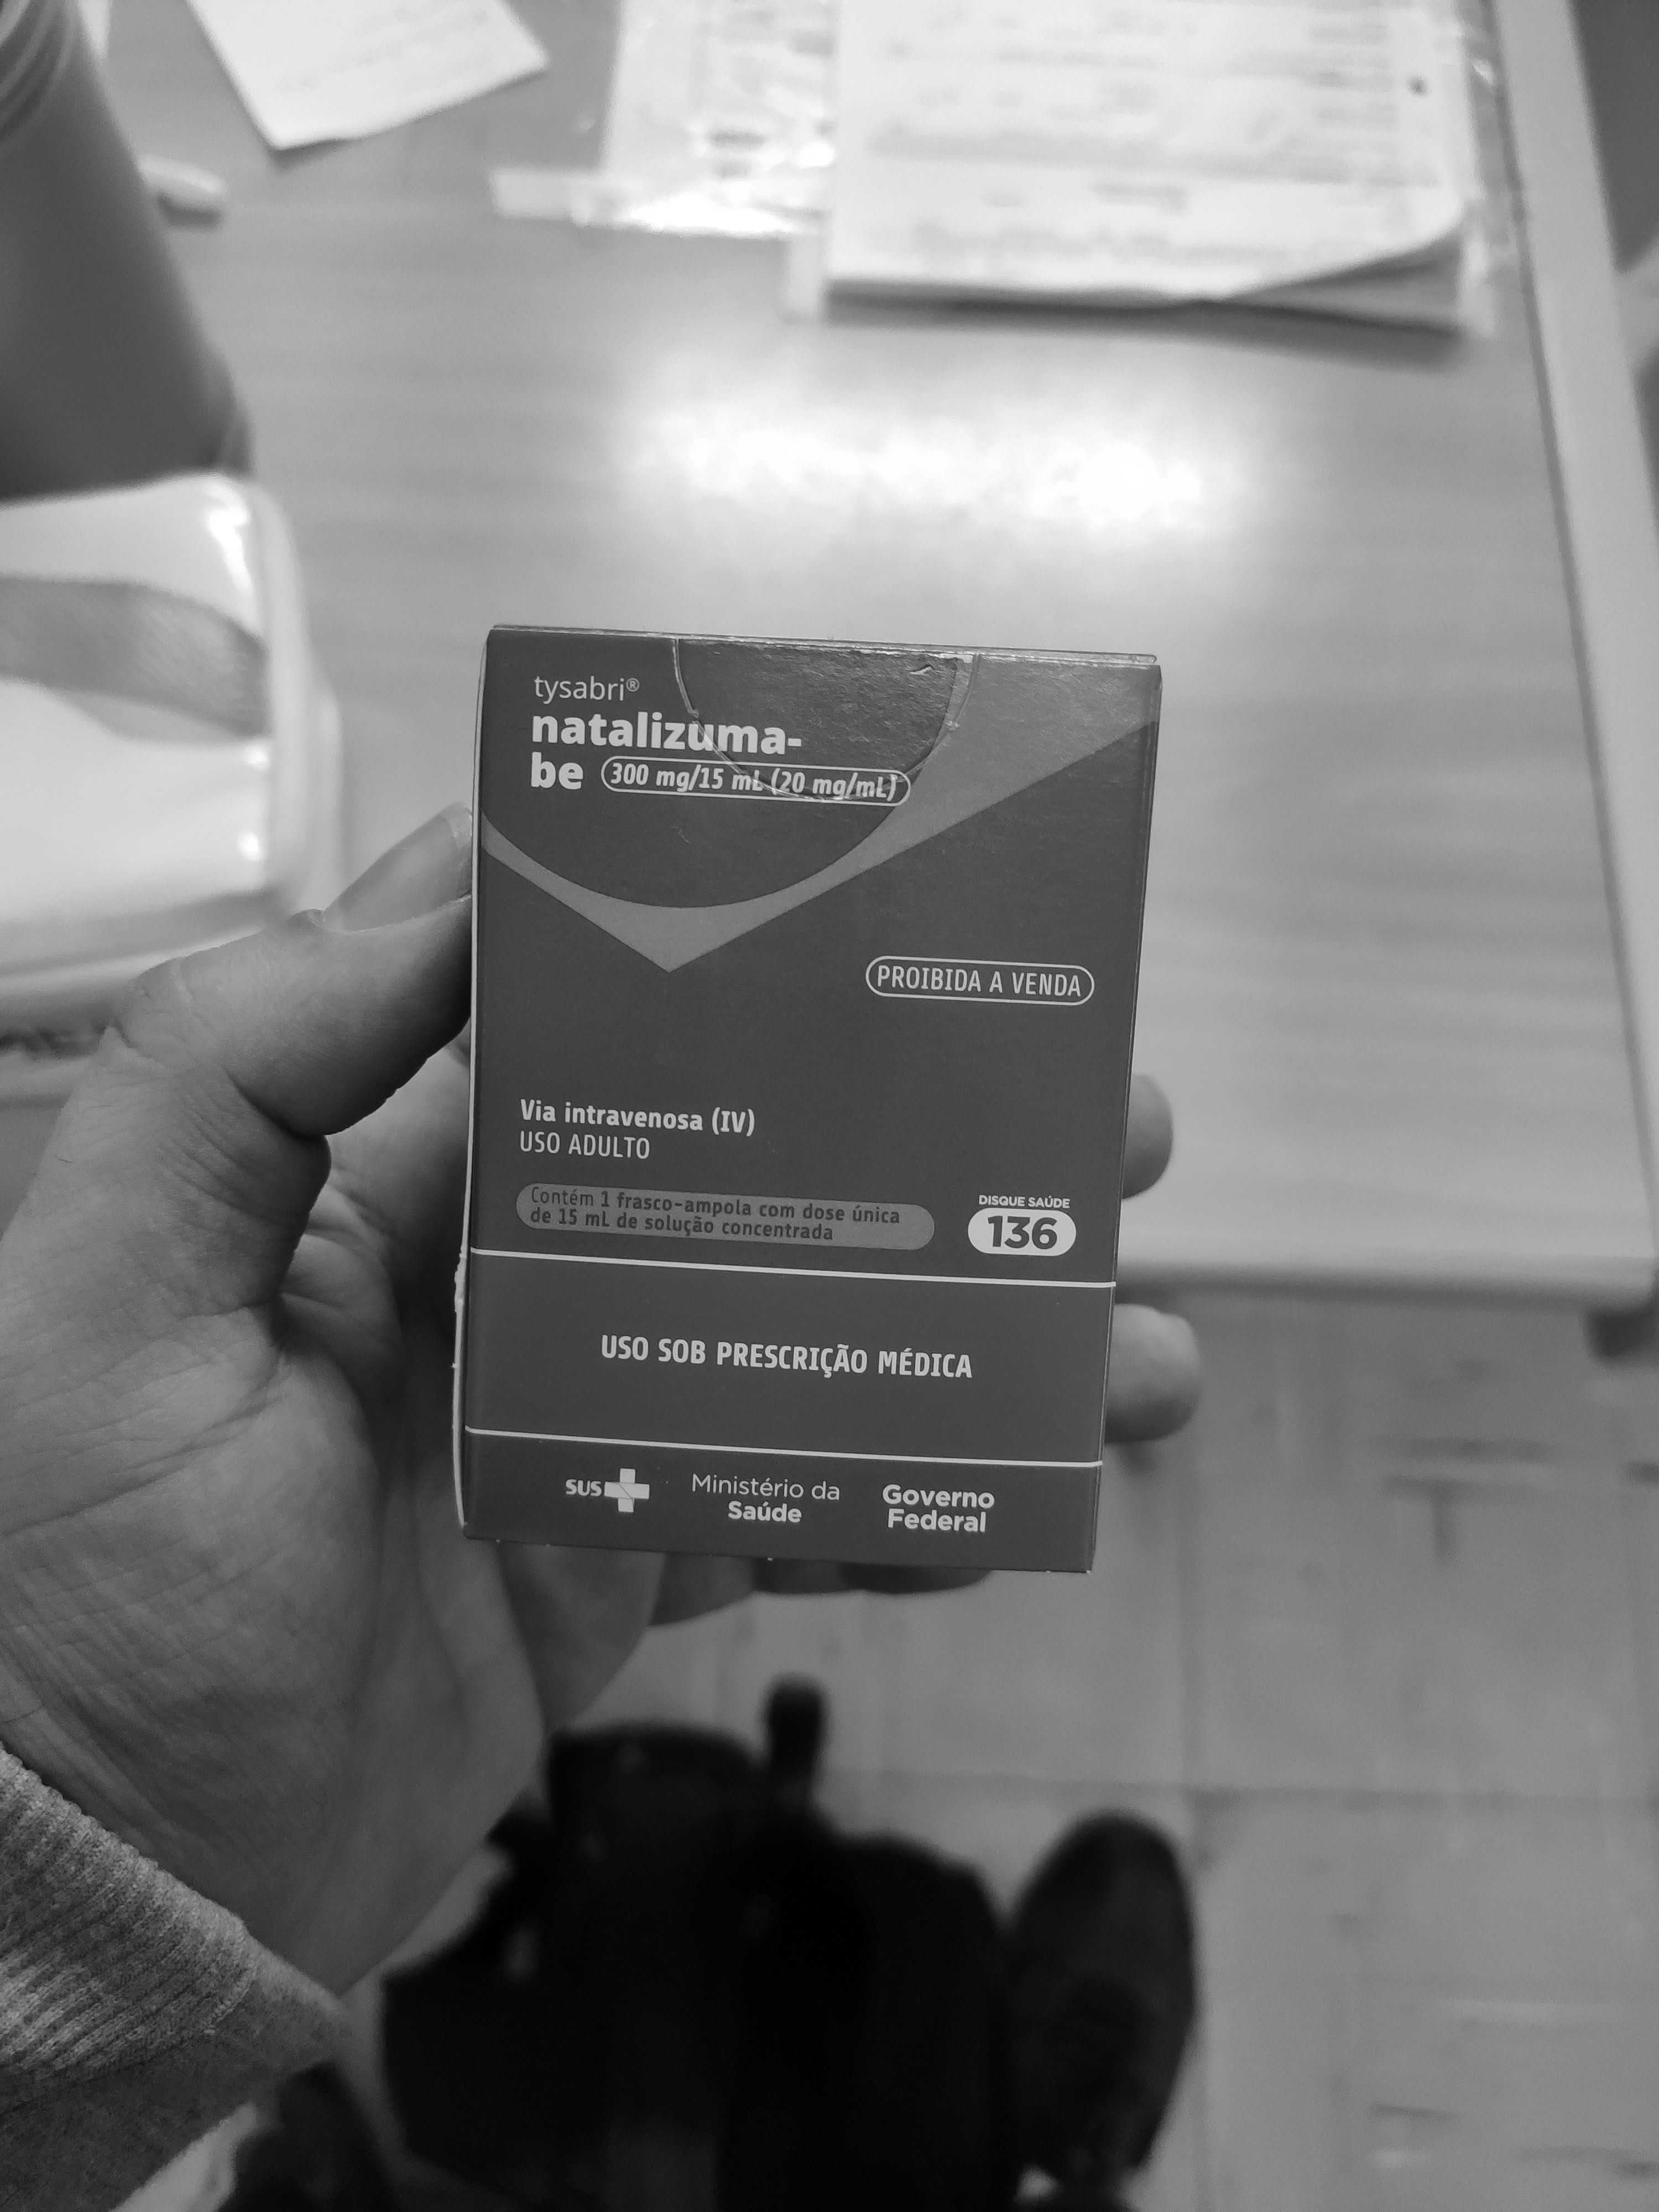
\includegraphics[width=\linewidth]{../pictures/tysabri_gray.jpg}
    \end{subfigure}
    \hfill
    \begin{subfigure}[t]{0.21\textwidth}
        \centering
        \caption{R.}
        \label{fig:foto:versoes:1:R}
        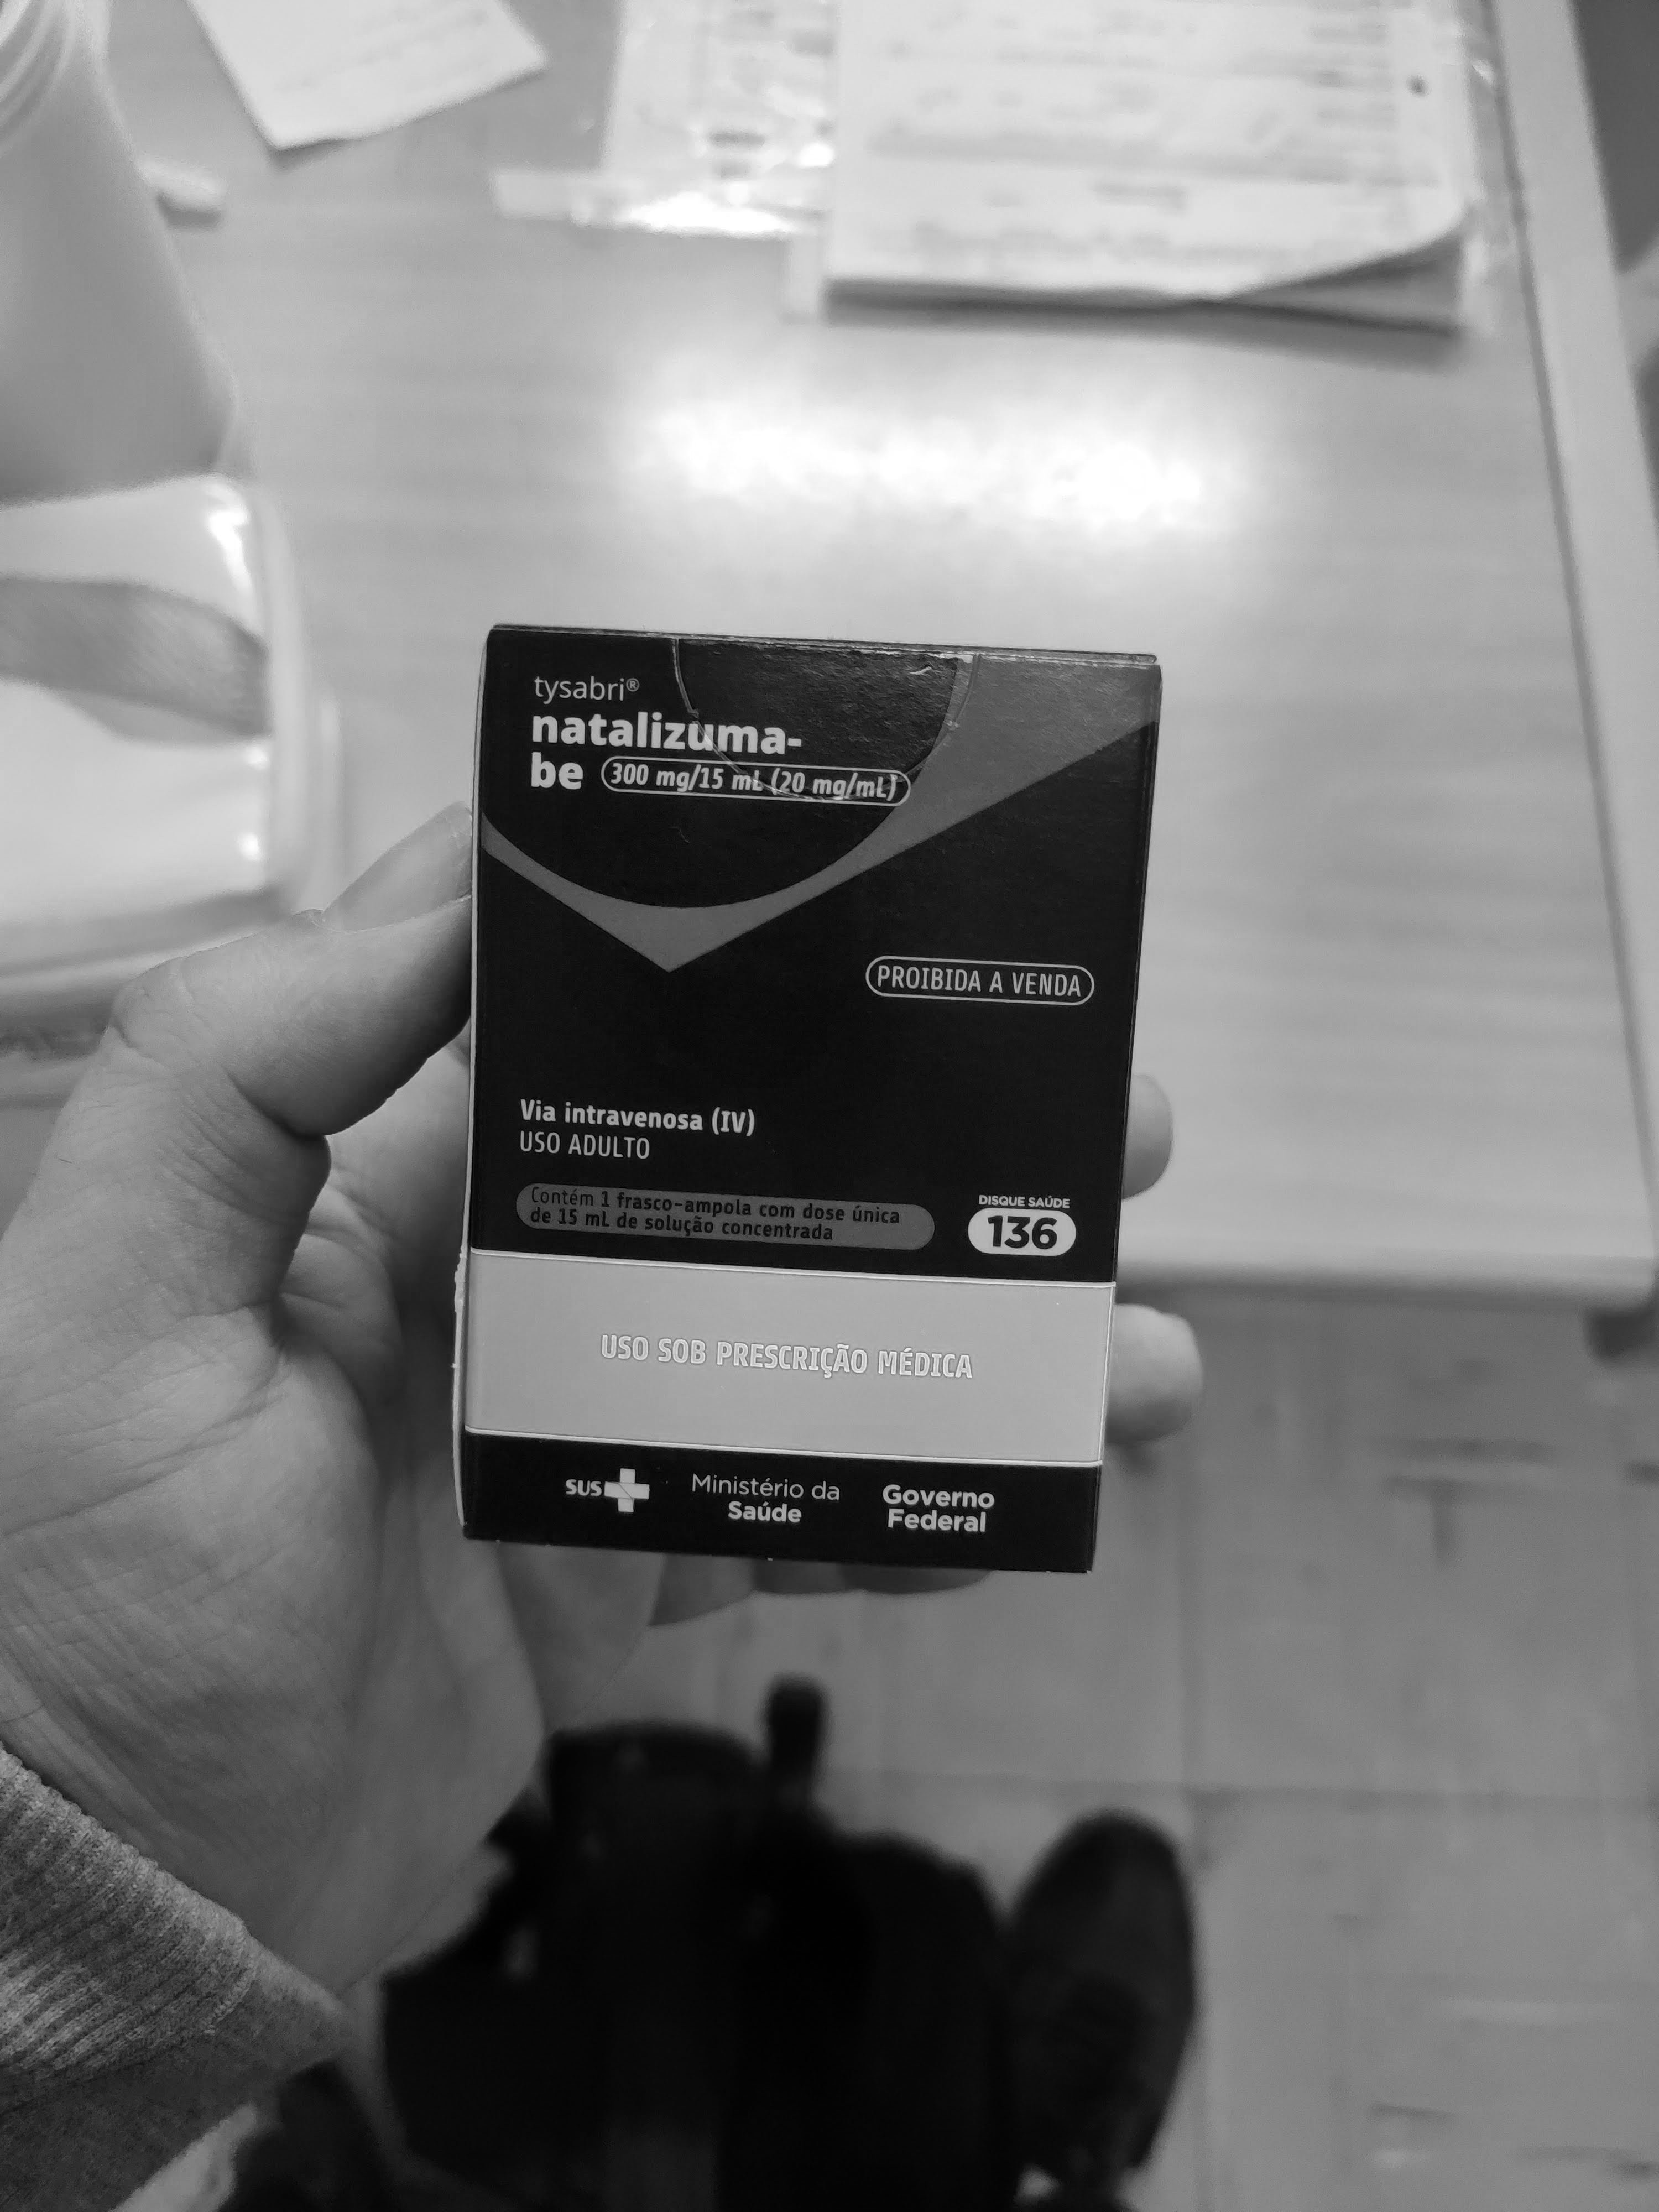
\includegraphics[width=\linewidth]{../pictures/tysabri_rgb_r_only.jpg}
    \end{subfigure}
    \hfill
    \begin{subfigure}[t]{0.21\textwidth}
        \centering
        \caption{G.}
        \label{fig:foto:versoes:1:G}
        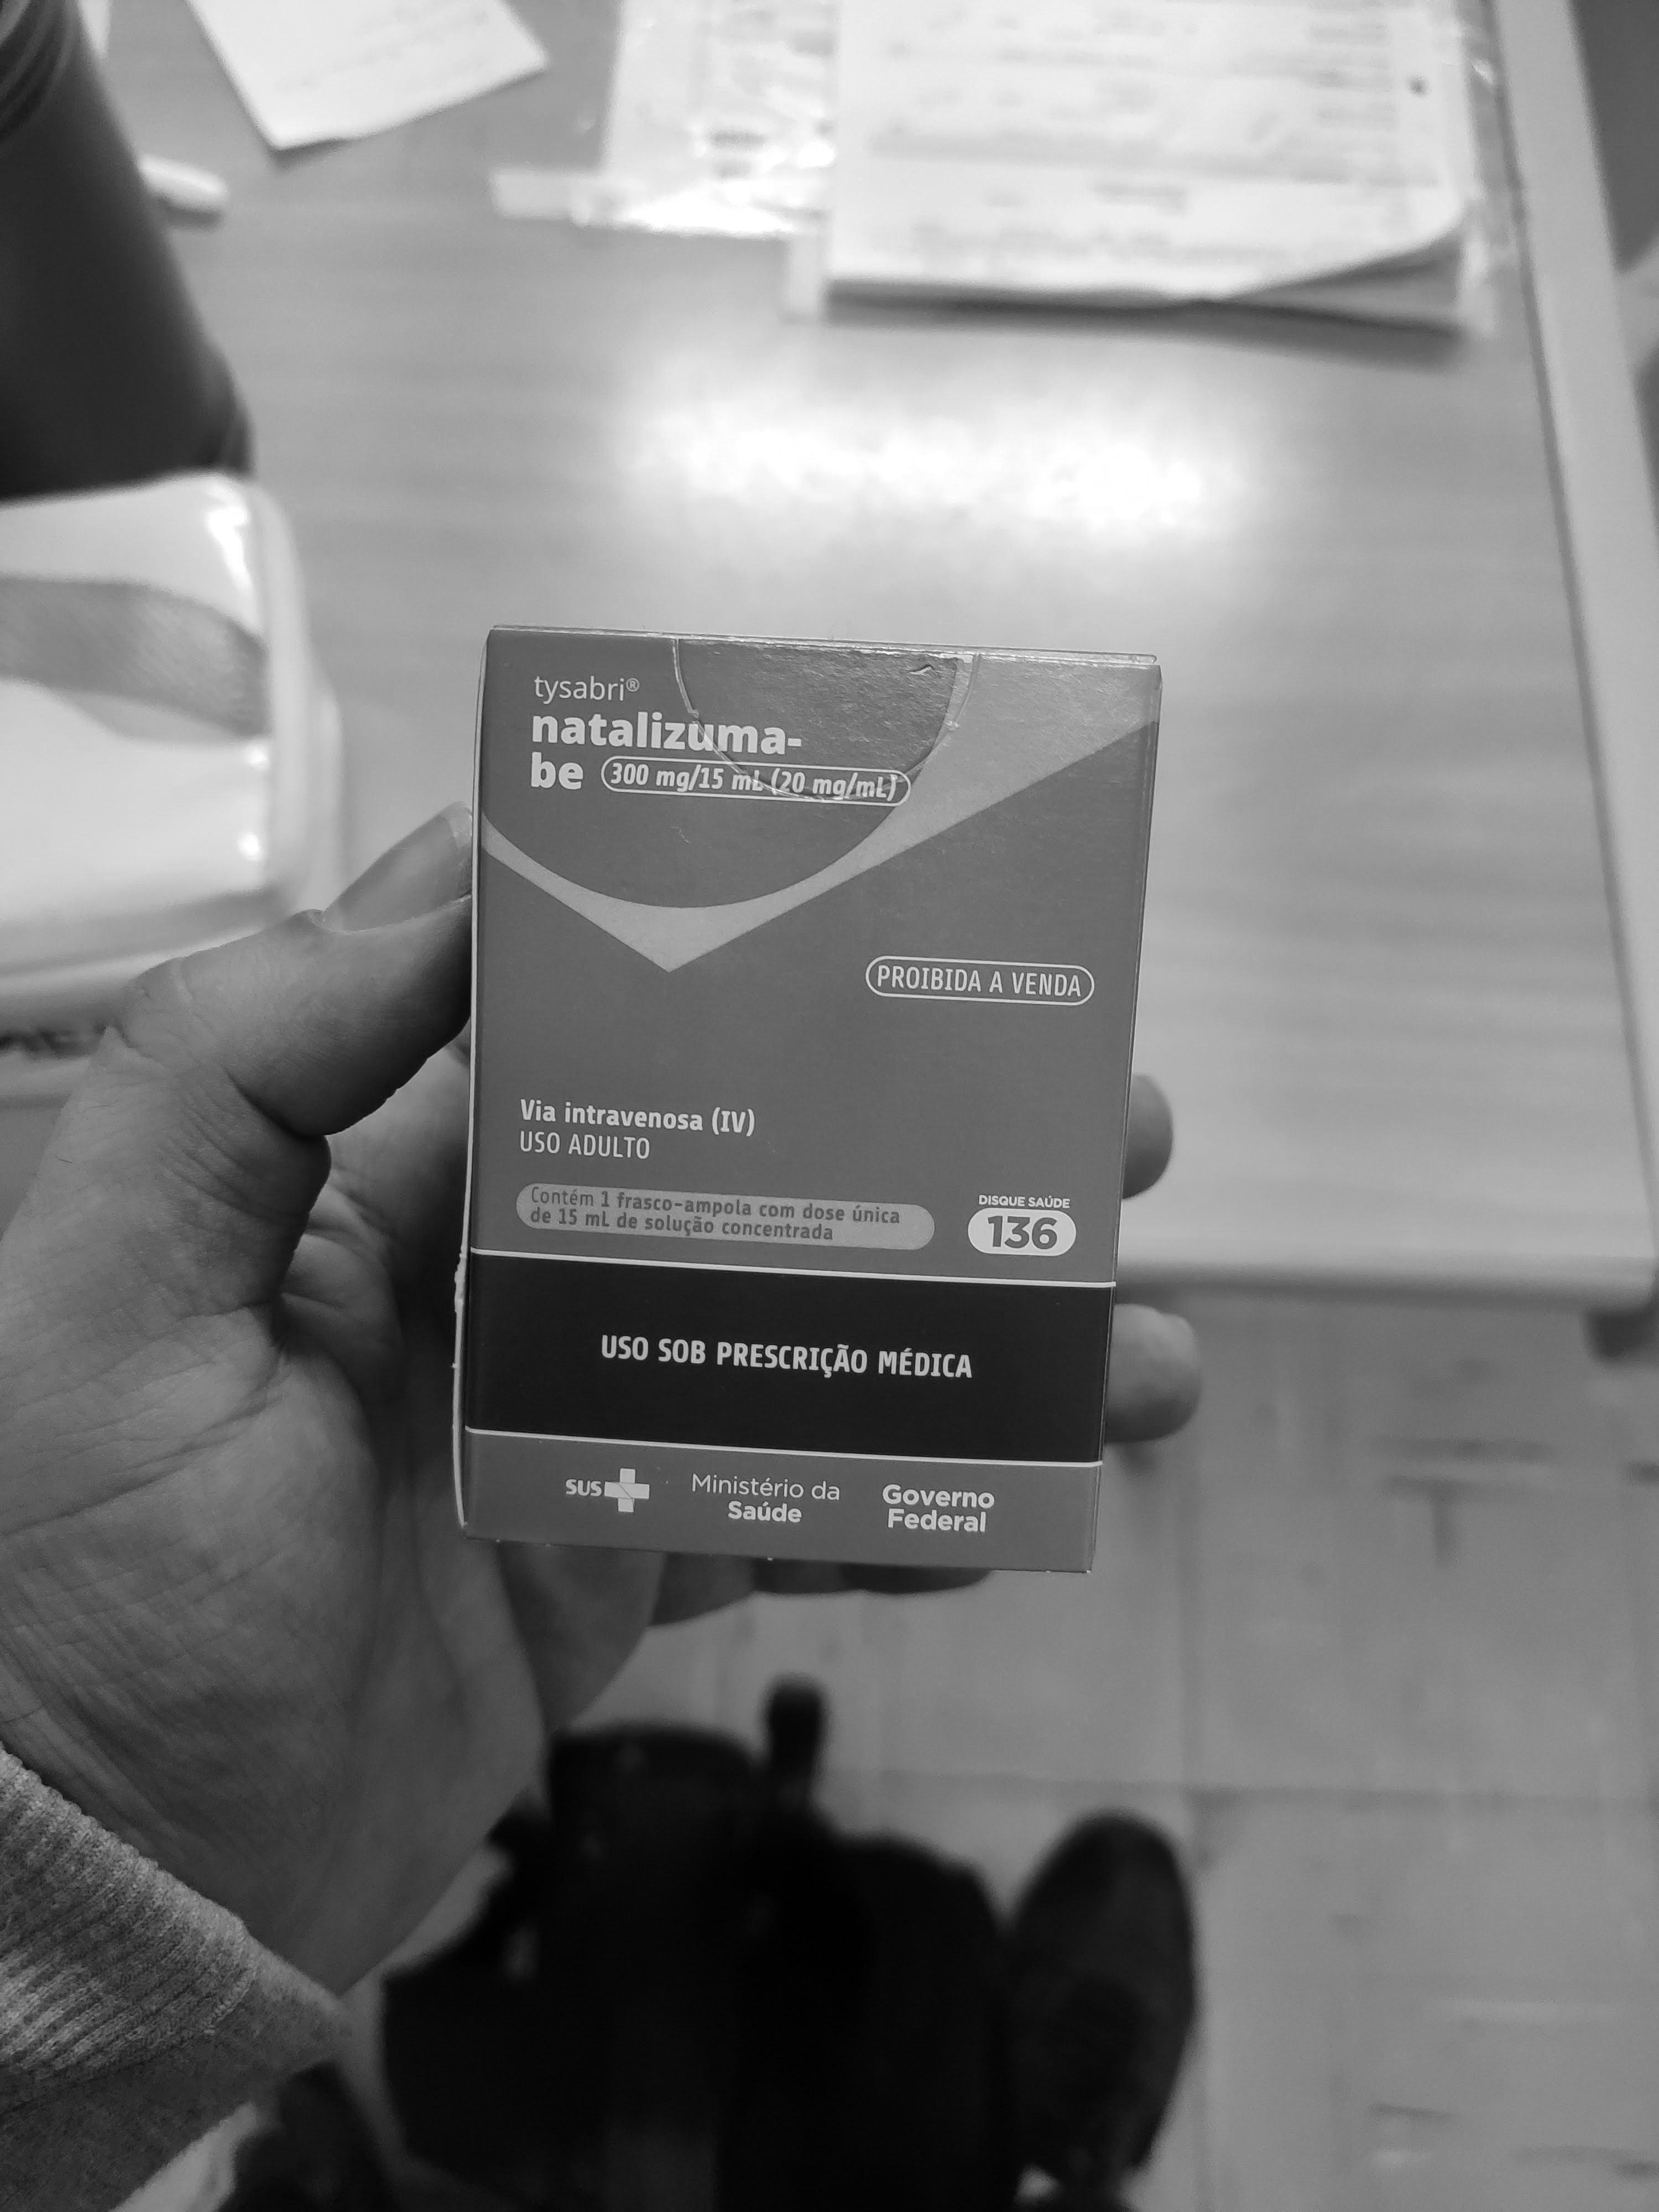
\includegraphics[width=\linewidth]{../pictures/tysabri_rgb_g_only.jpg}
    \end{subfigure}
    \hfill
    \begin{subfigure}[t]{0.21\textwidth}
        \centering
        \caption{B.}
        \label{fig:foto:versoes:1:B}
        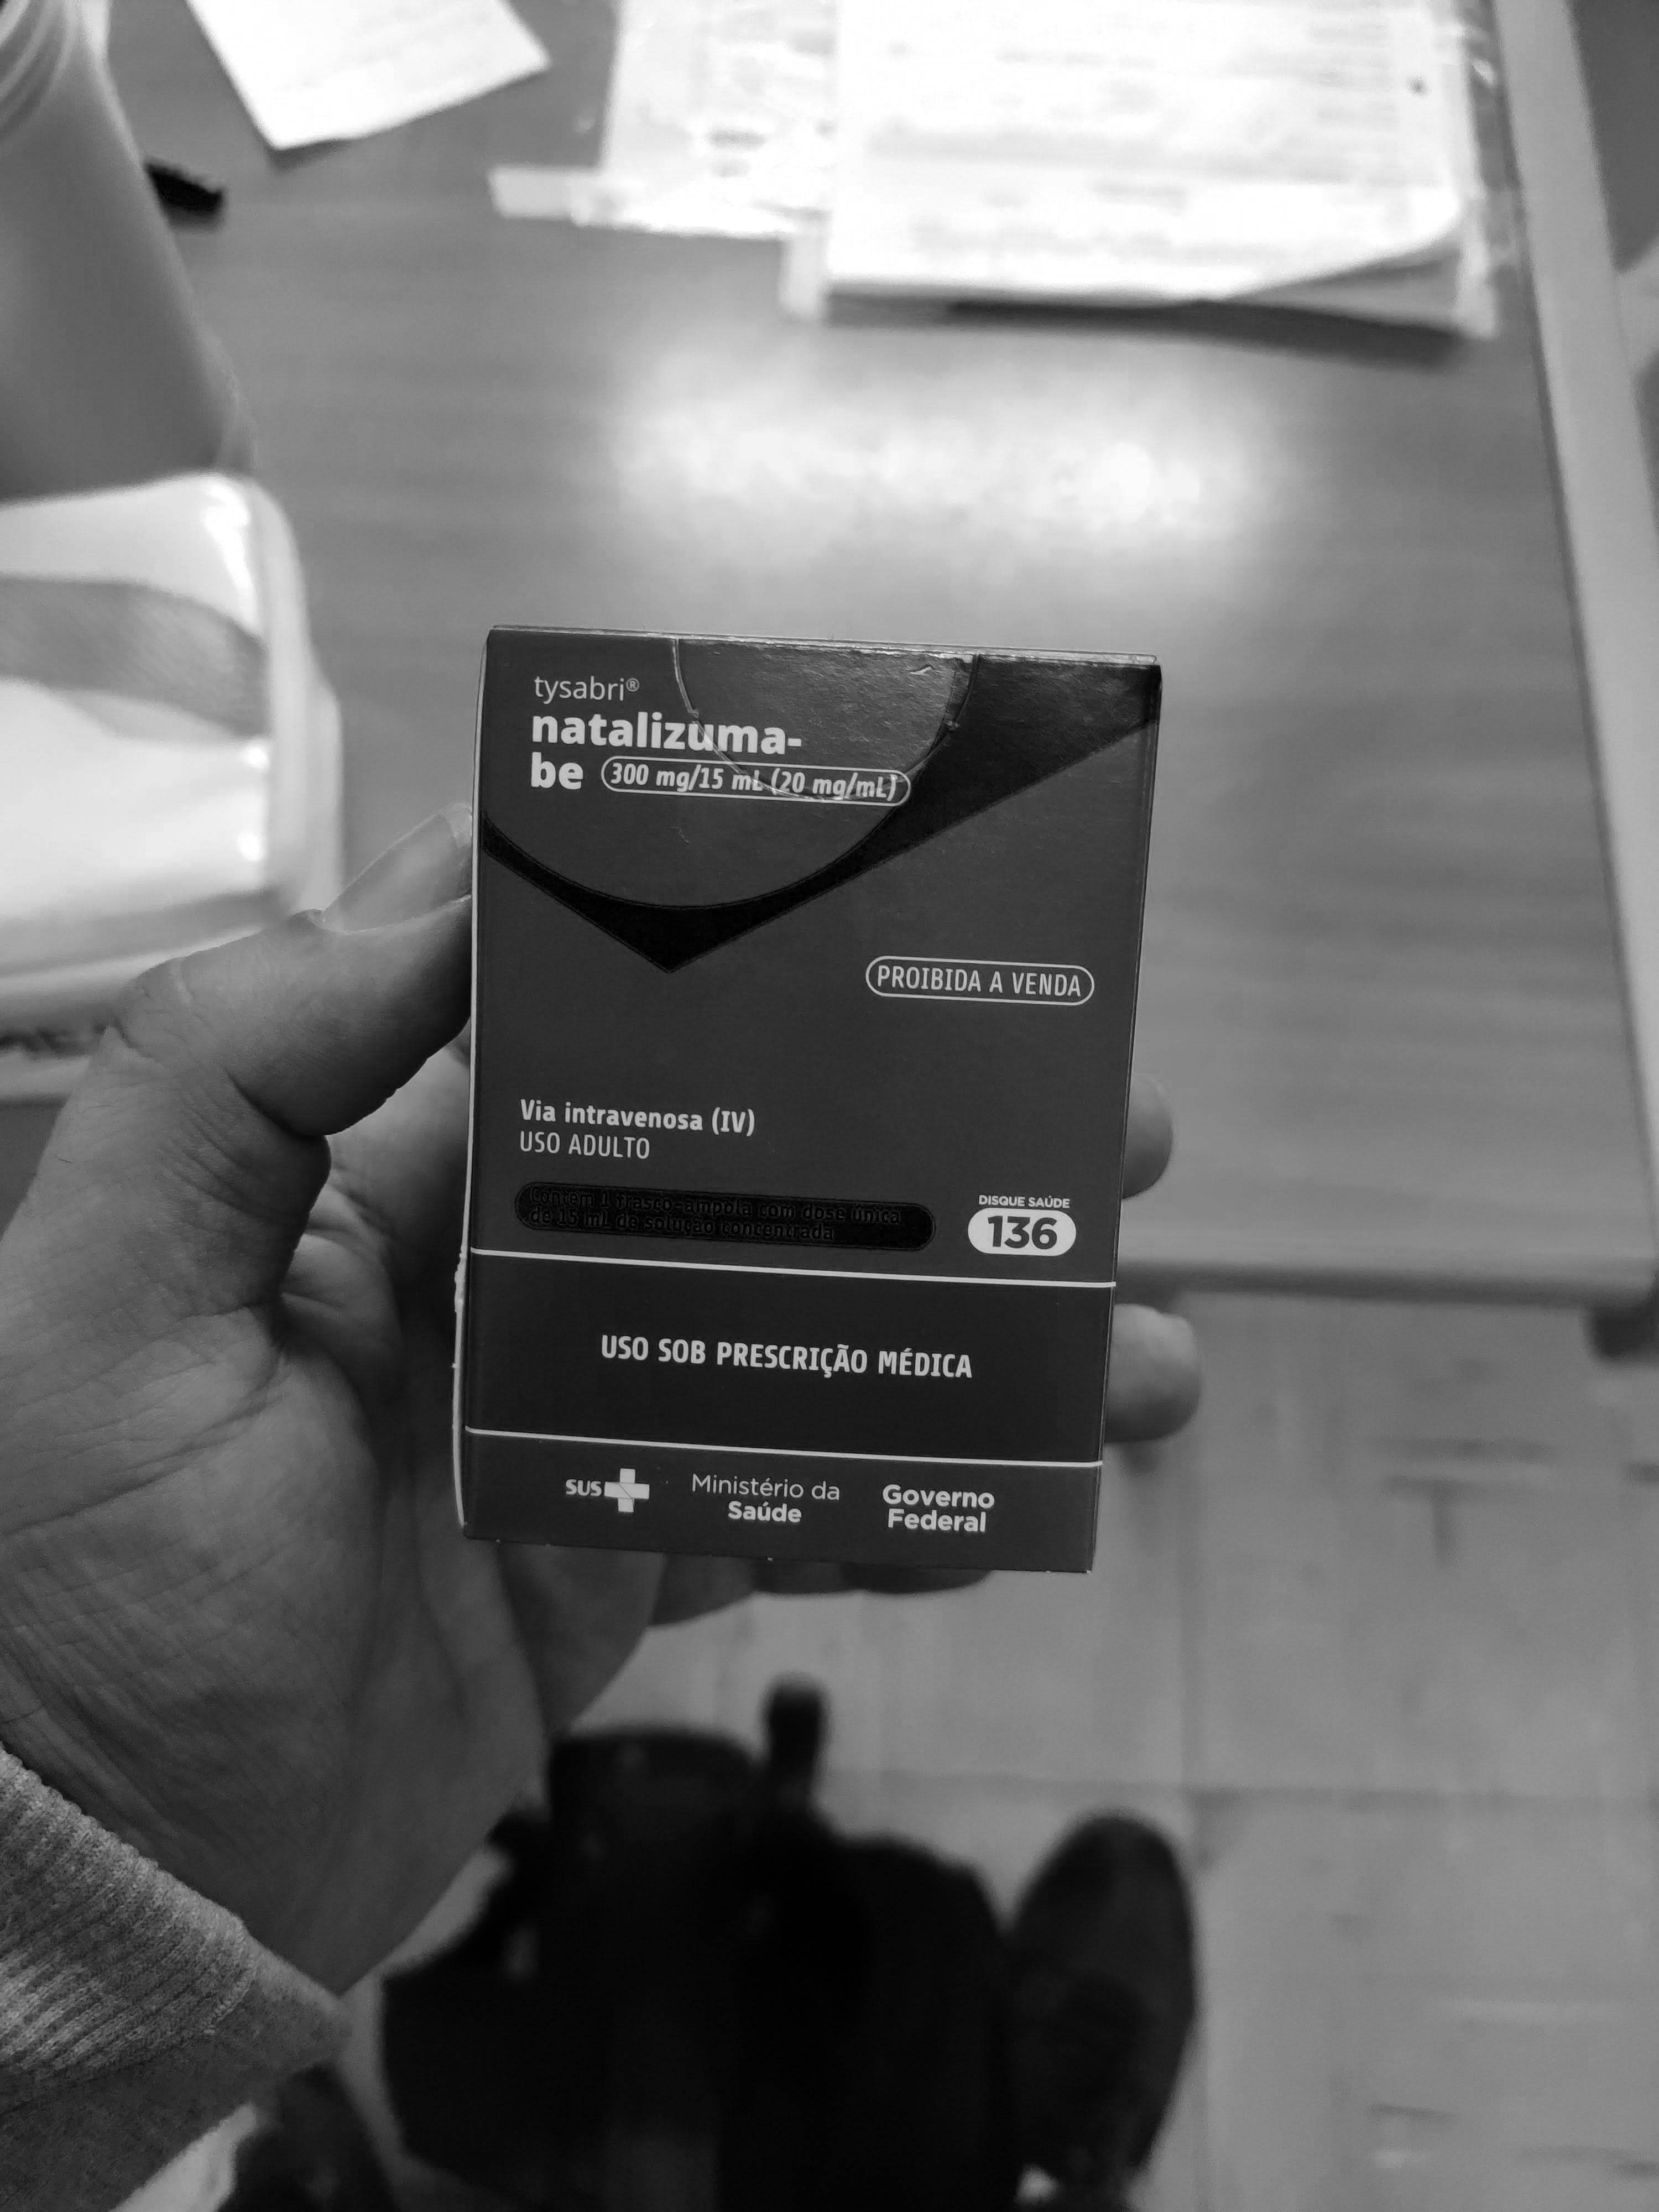
\includegraphics[width=\linewidth]{../pictures/tysabri_rgb_b_only.jpg}
    \end{subfigure}
    \\\vspace{\floatsep}
    \begin{subfigure}[t]{0.21\textwidth}
        \centering
        \caption{Cinza.}
        \label{fig:foto:versoes:1:Cinza:boxes}
        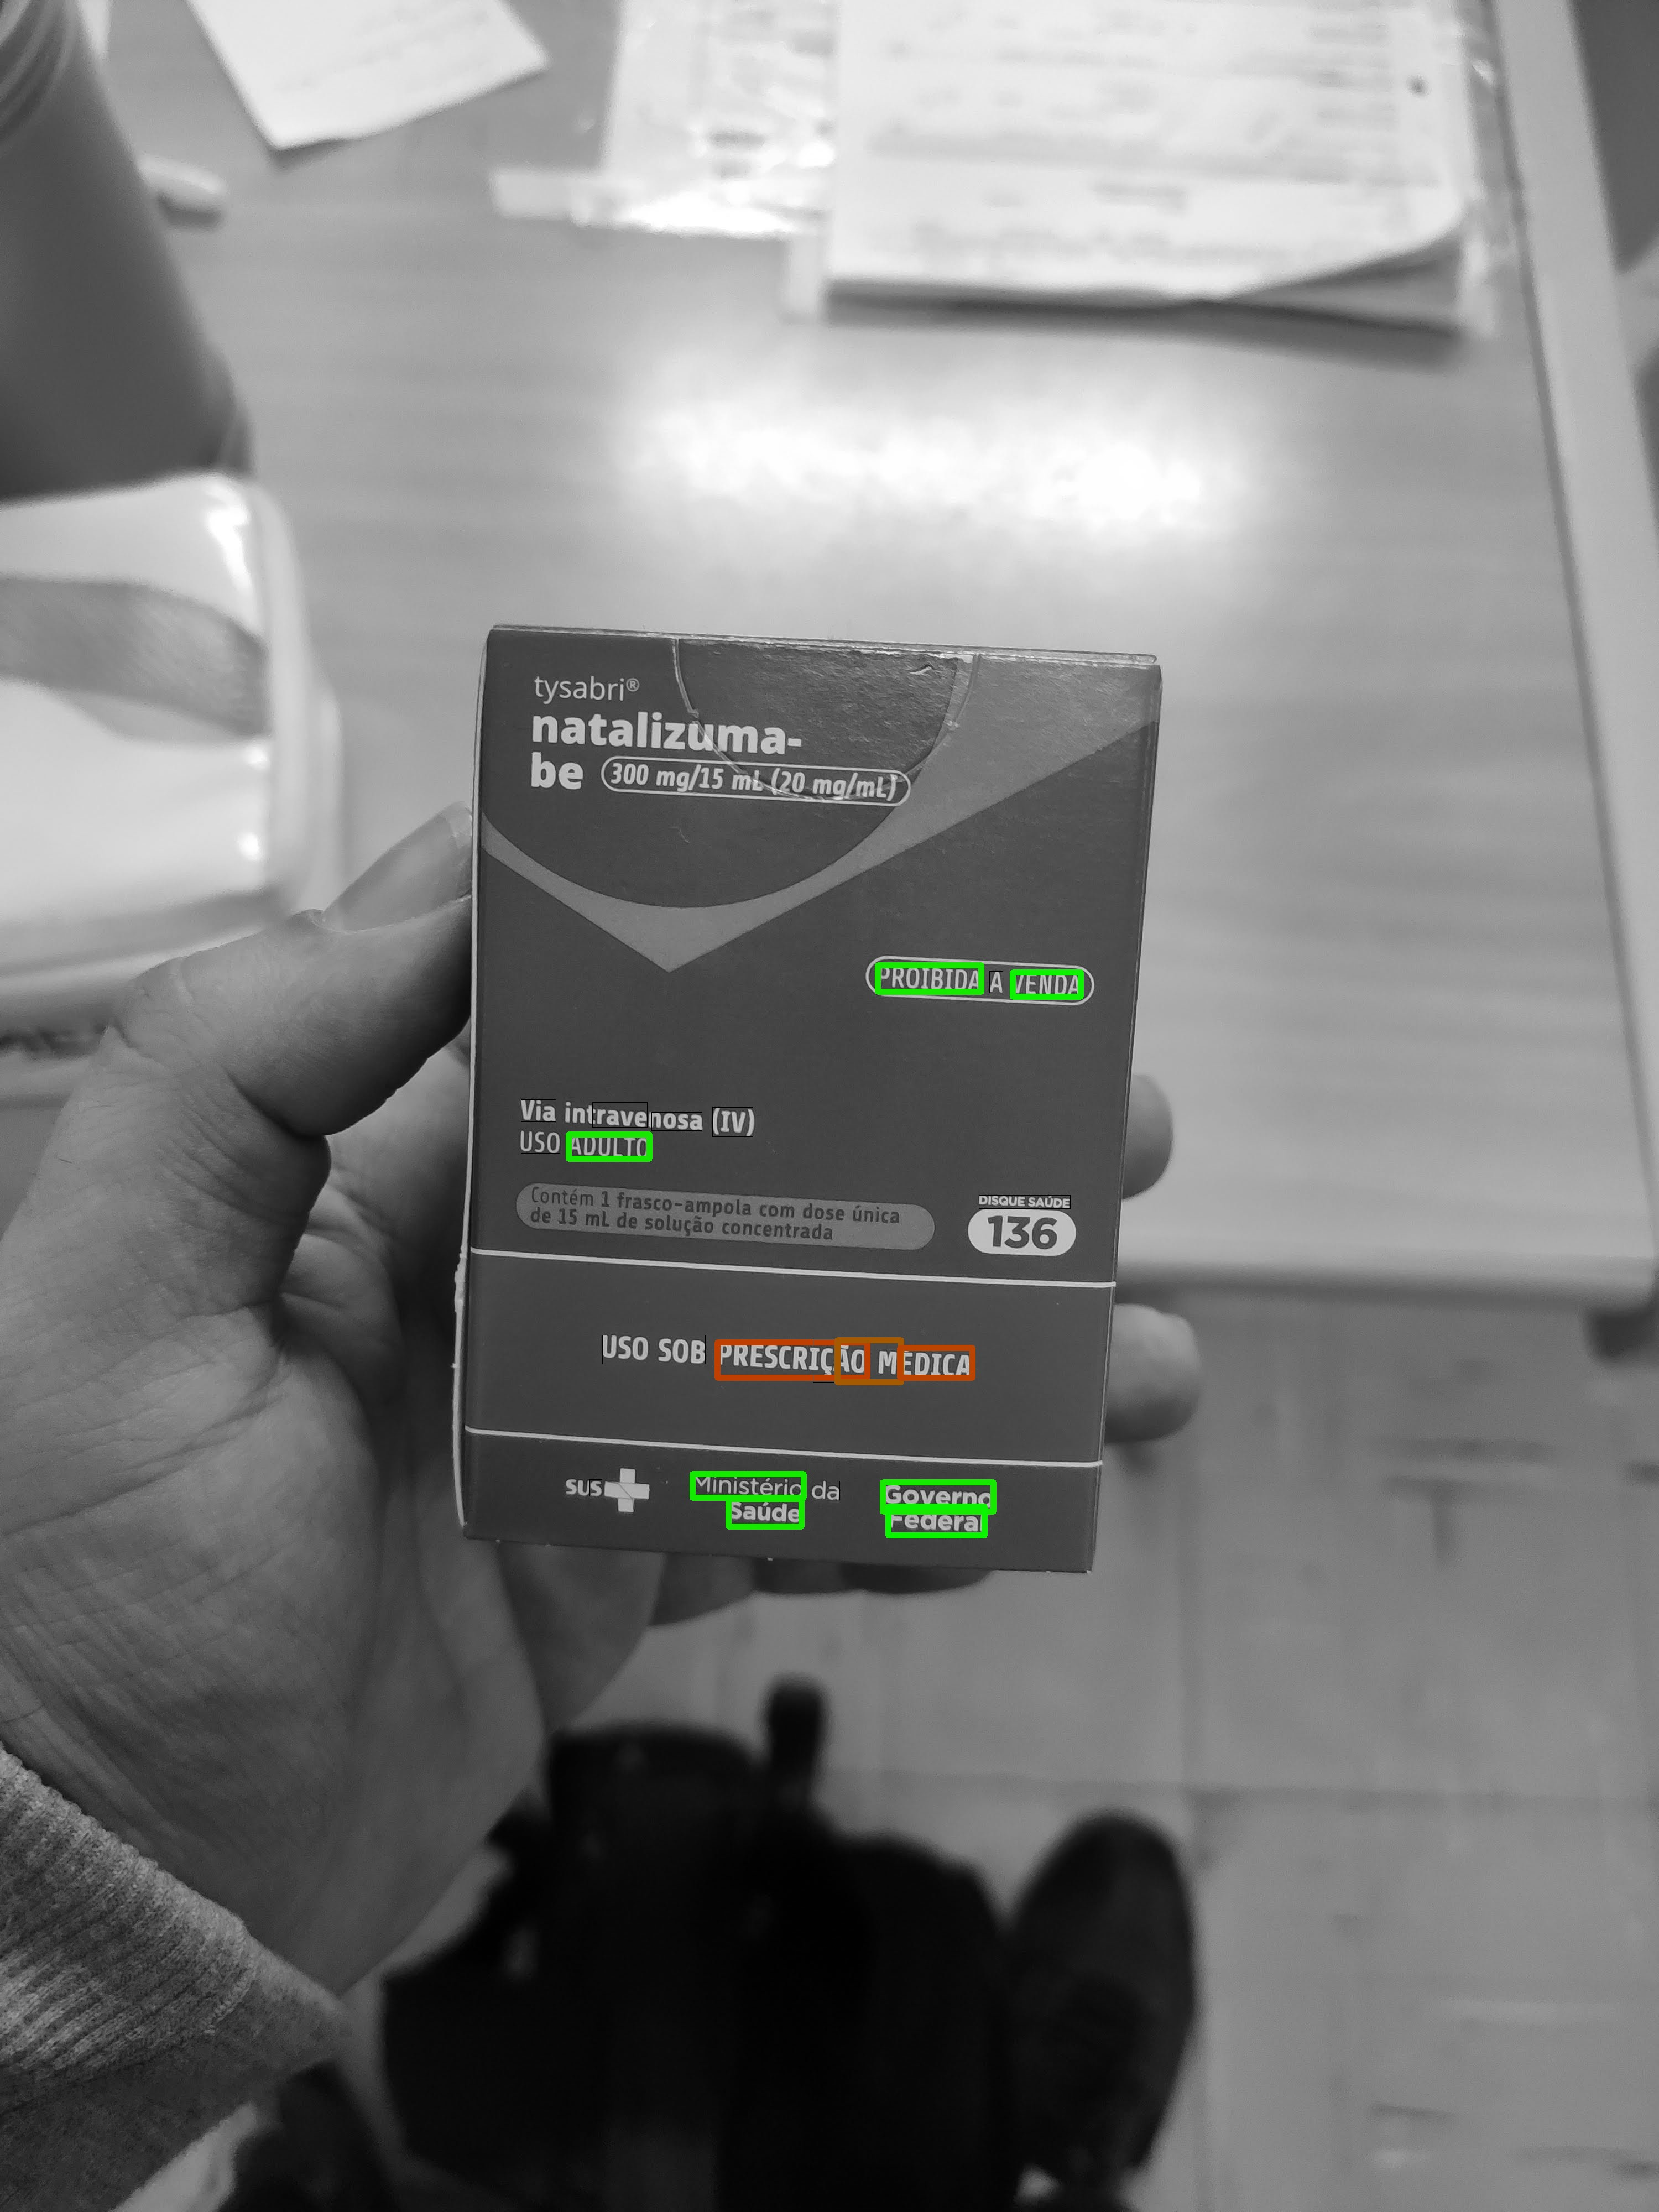
\includegraphics[width=\linewidth]{../pictures/tysabri_gray_boxes.jpg}
    \end{subfigure}
    \hfill
    \begin{subfigure}[t]{0.21\textwidth}
        \centering
        \caption{R.}
        \label{fig:foto:versoes:1:R:boxes}
        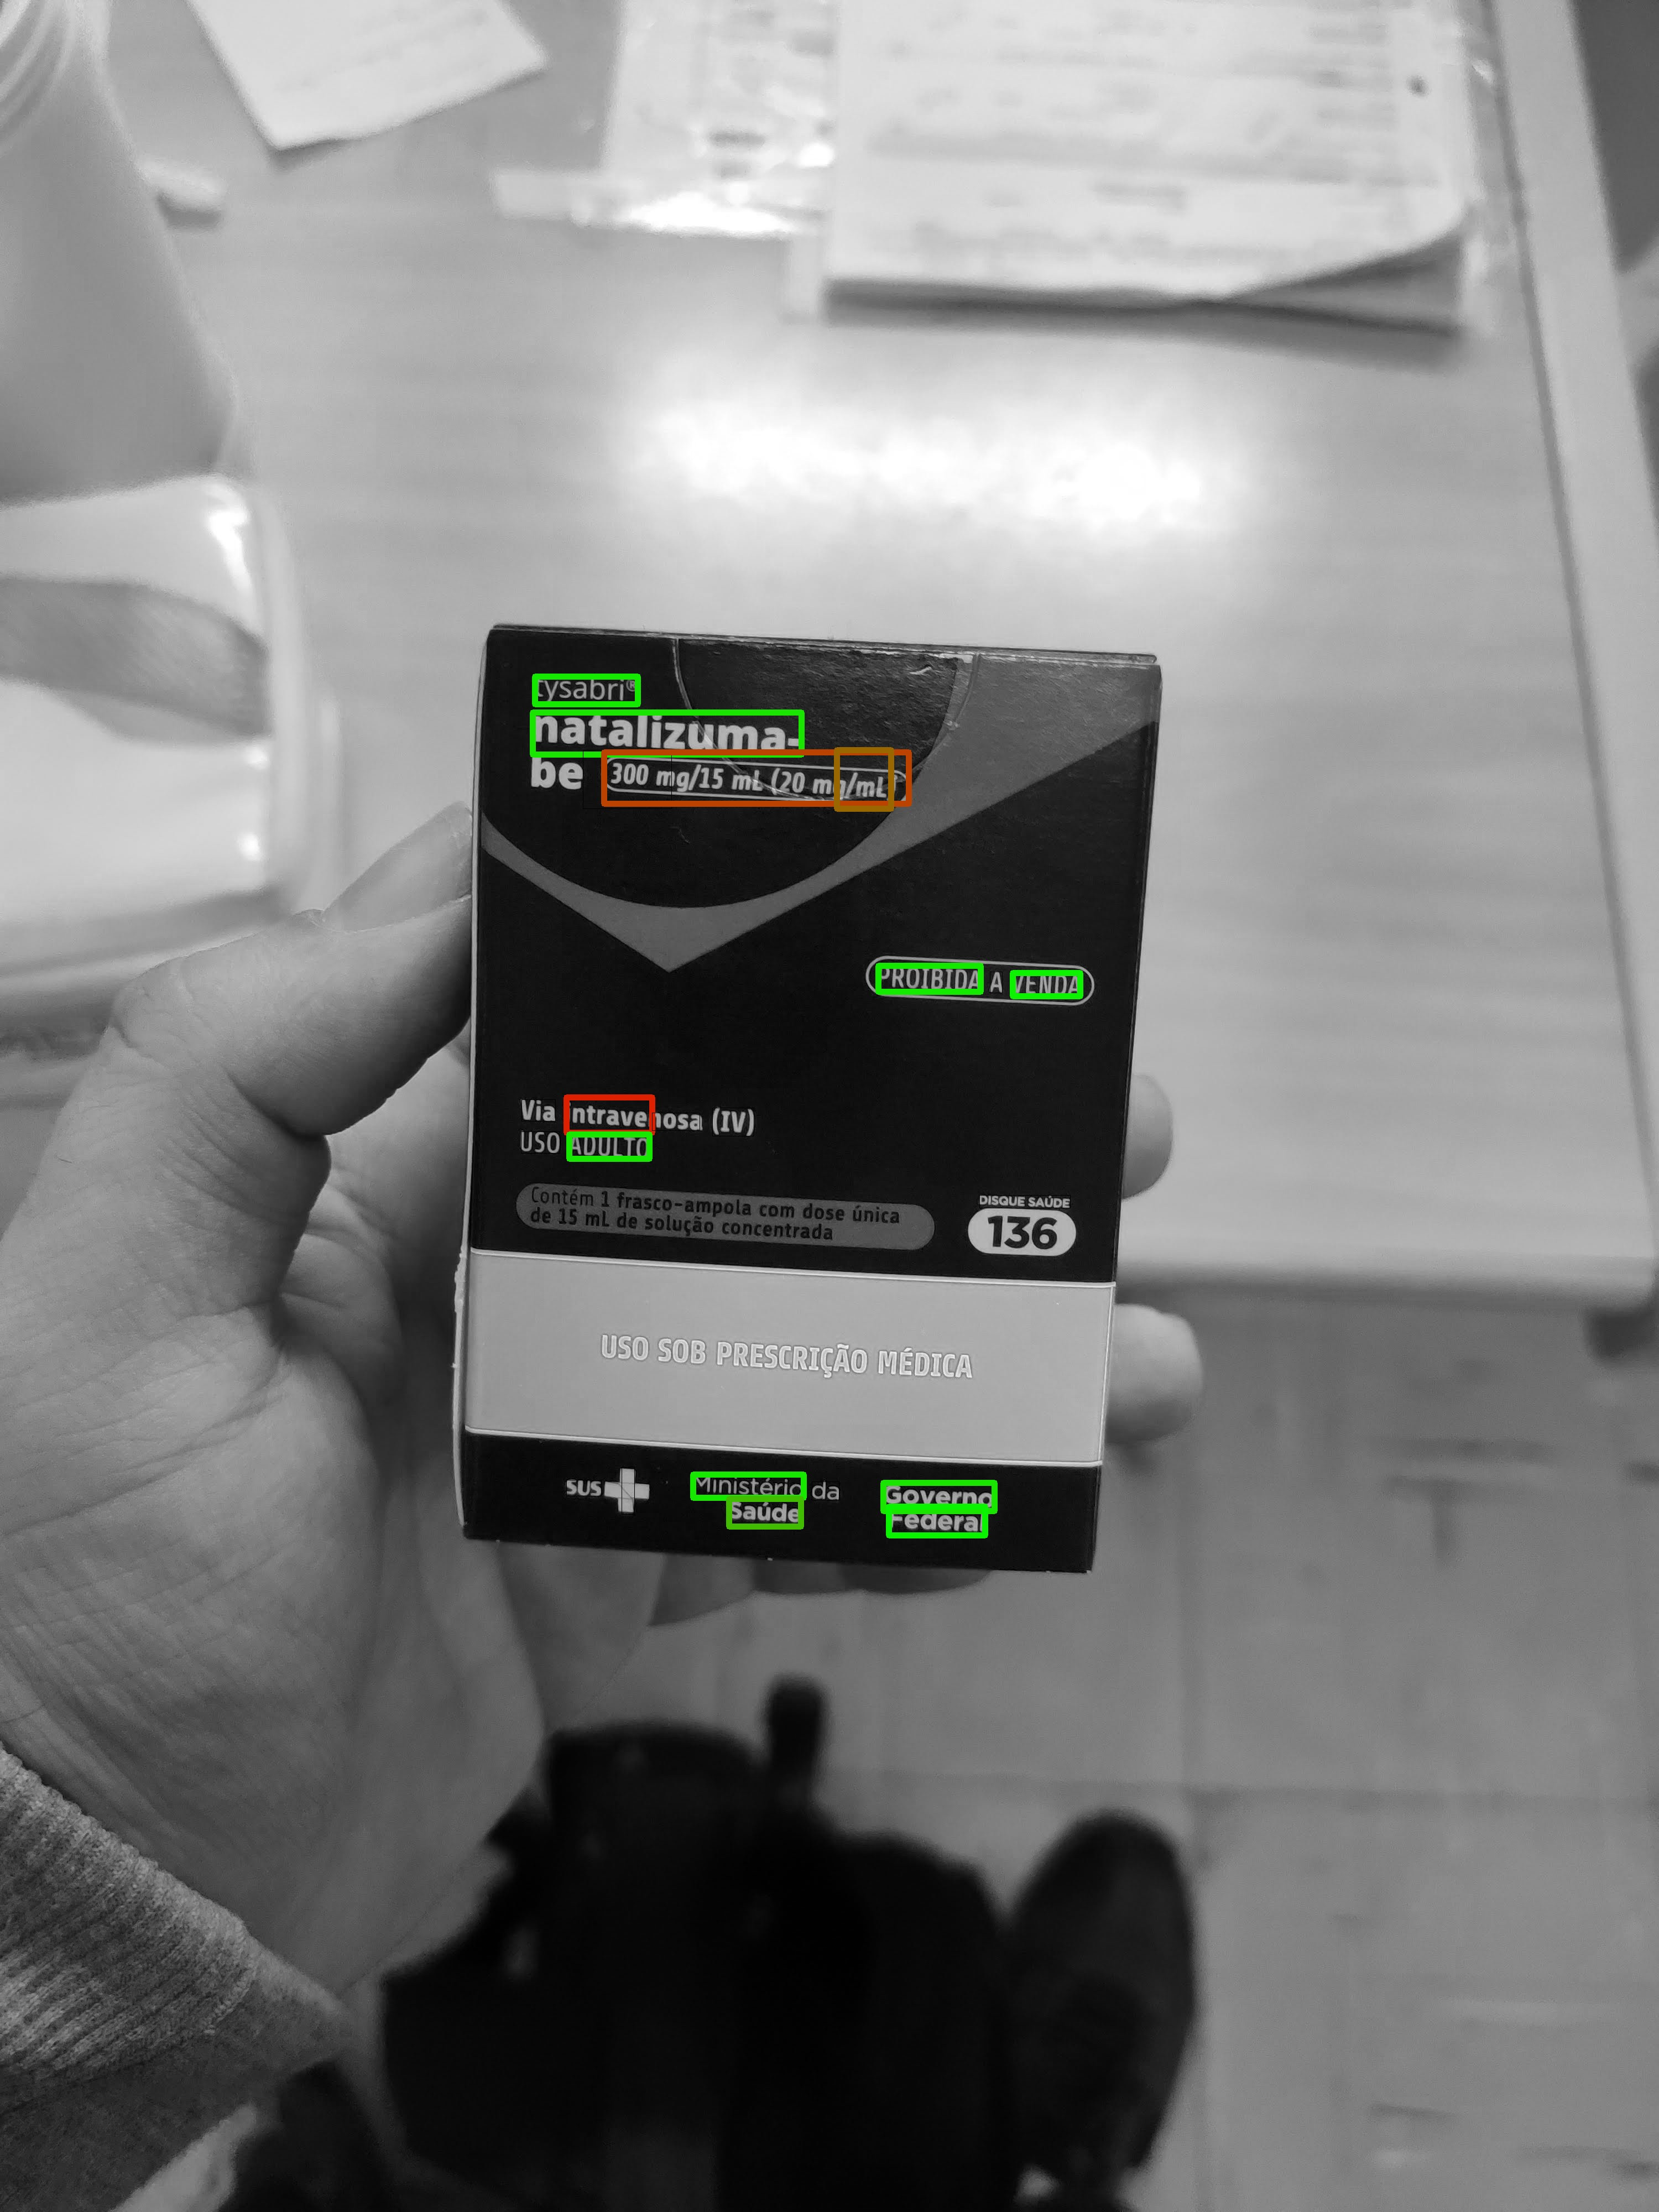
\includegraphics[width=\linewidth]{../pictures/tysabri_rgb_r_only_boxes.jpg}
    \end{subfigure}
    \hfill
    \begin{subfigure}[t]{0.21\textwidth}
        \centering
        \caption{G.}
        \label{fig:foto:versoes:1:G:boxes}
        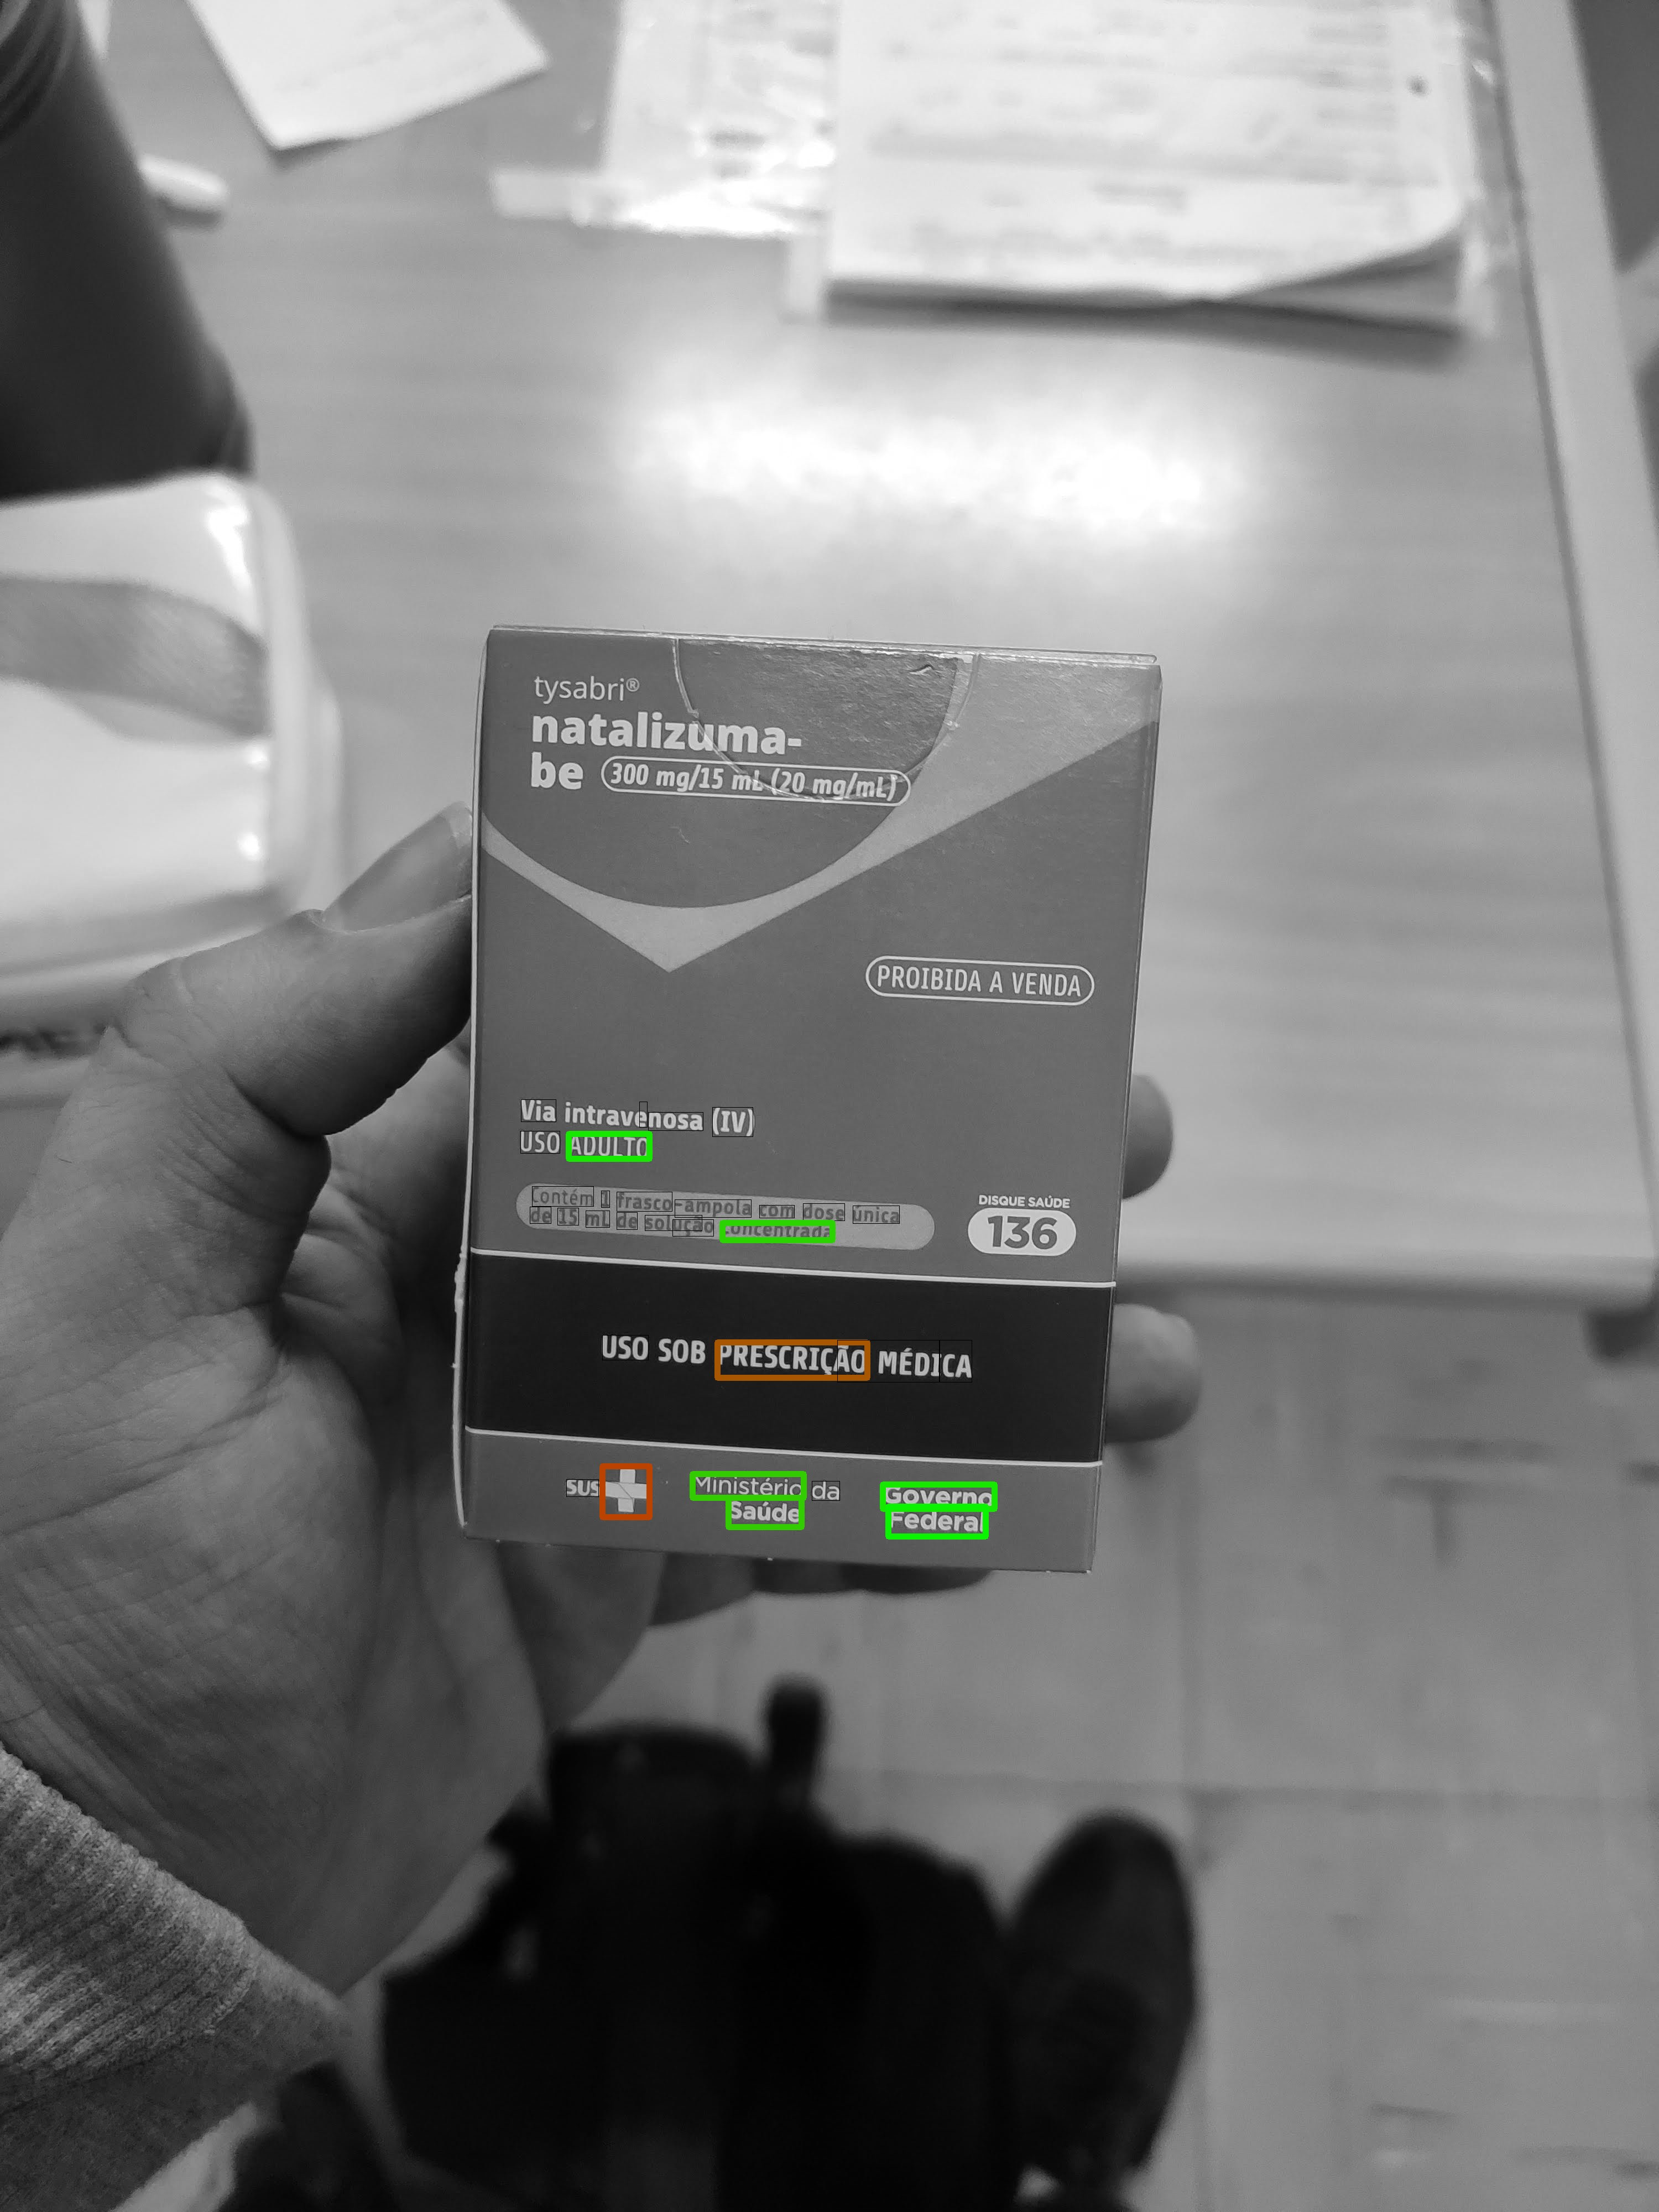
\includegraphics[width=\linewidth]{../pictures/tysabri_rgb_g_only_boxes.jpg}
    \end{subfigure}
    \hfill
    \begin{subfigure}[t]{0.21\textwidth}
        \centering
        \caption{B.}
        \label{fig:foto:versoes:1:B:boxes}
        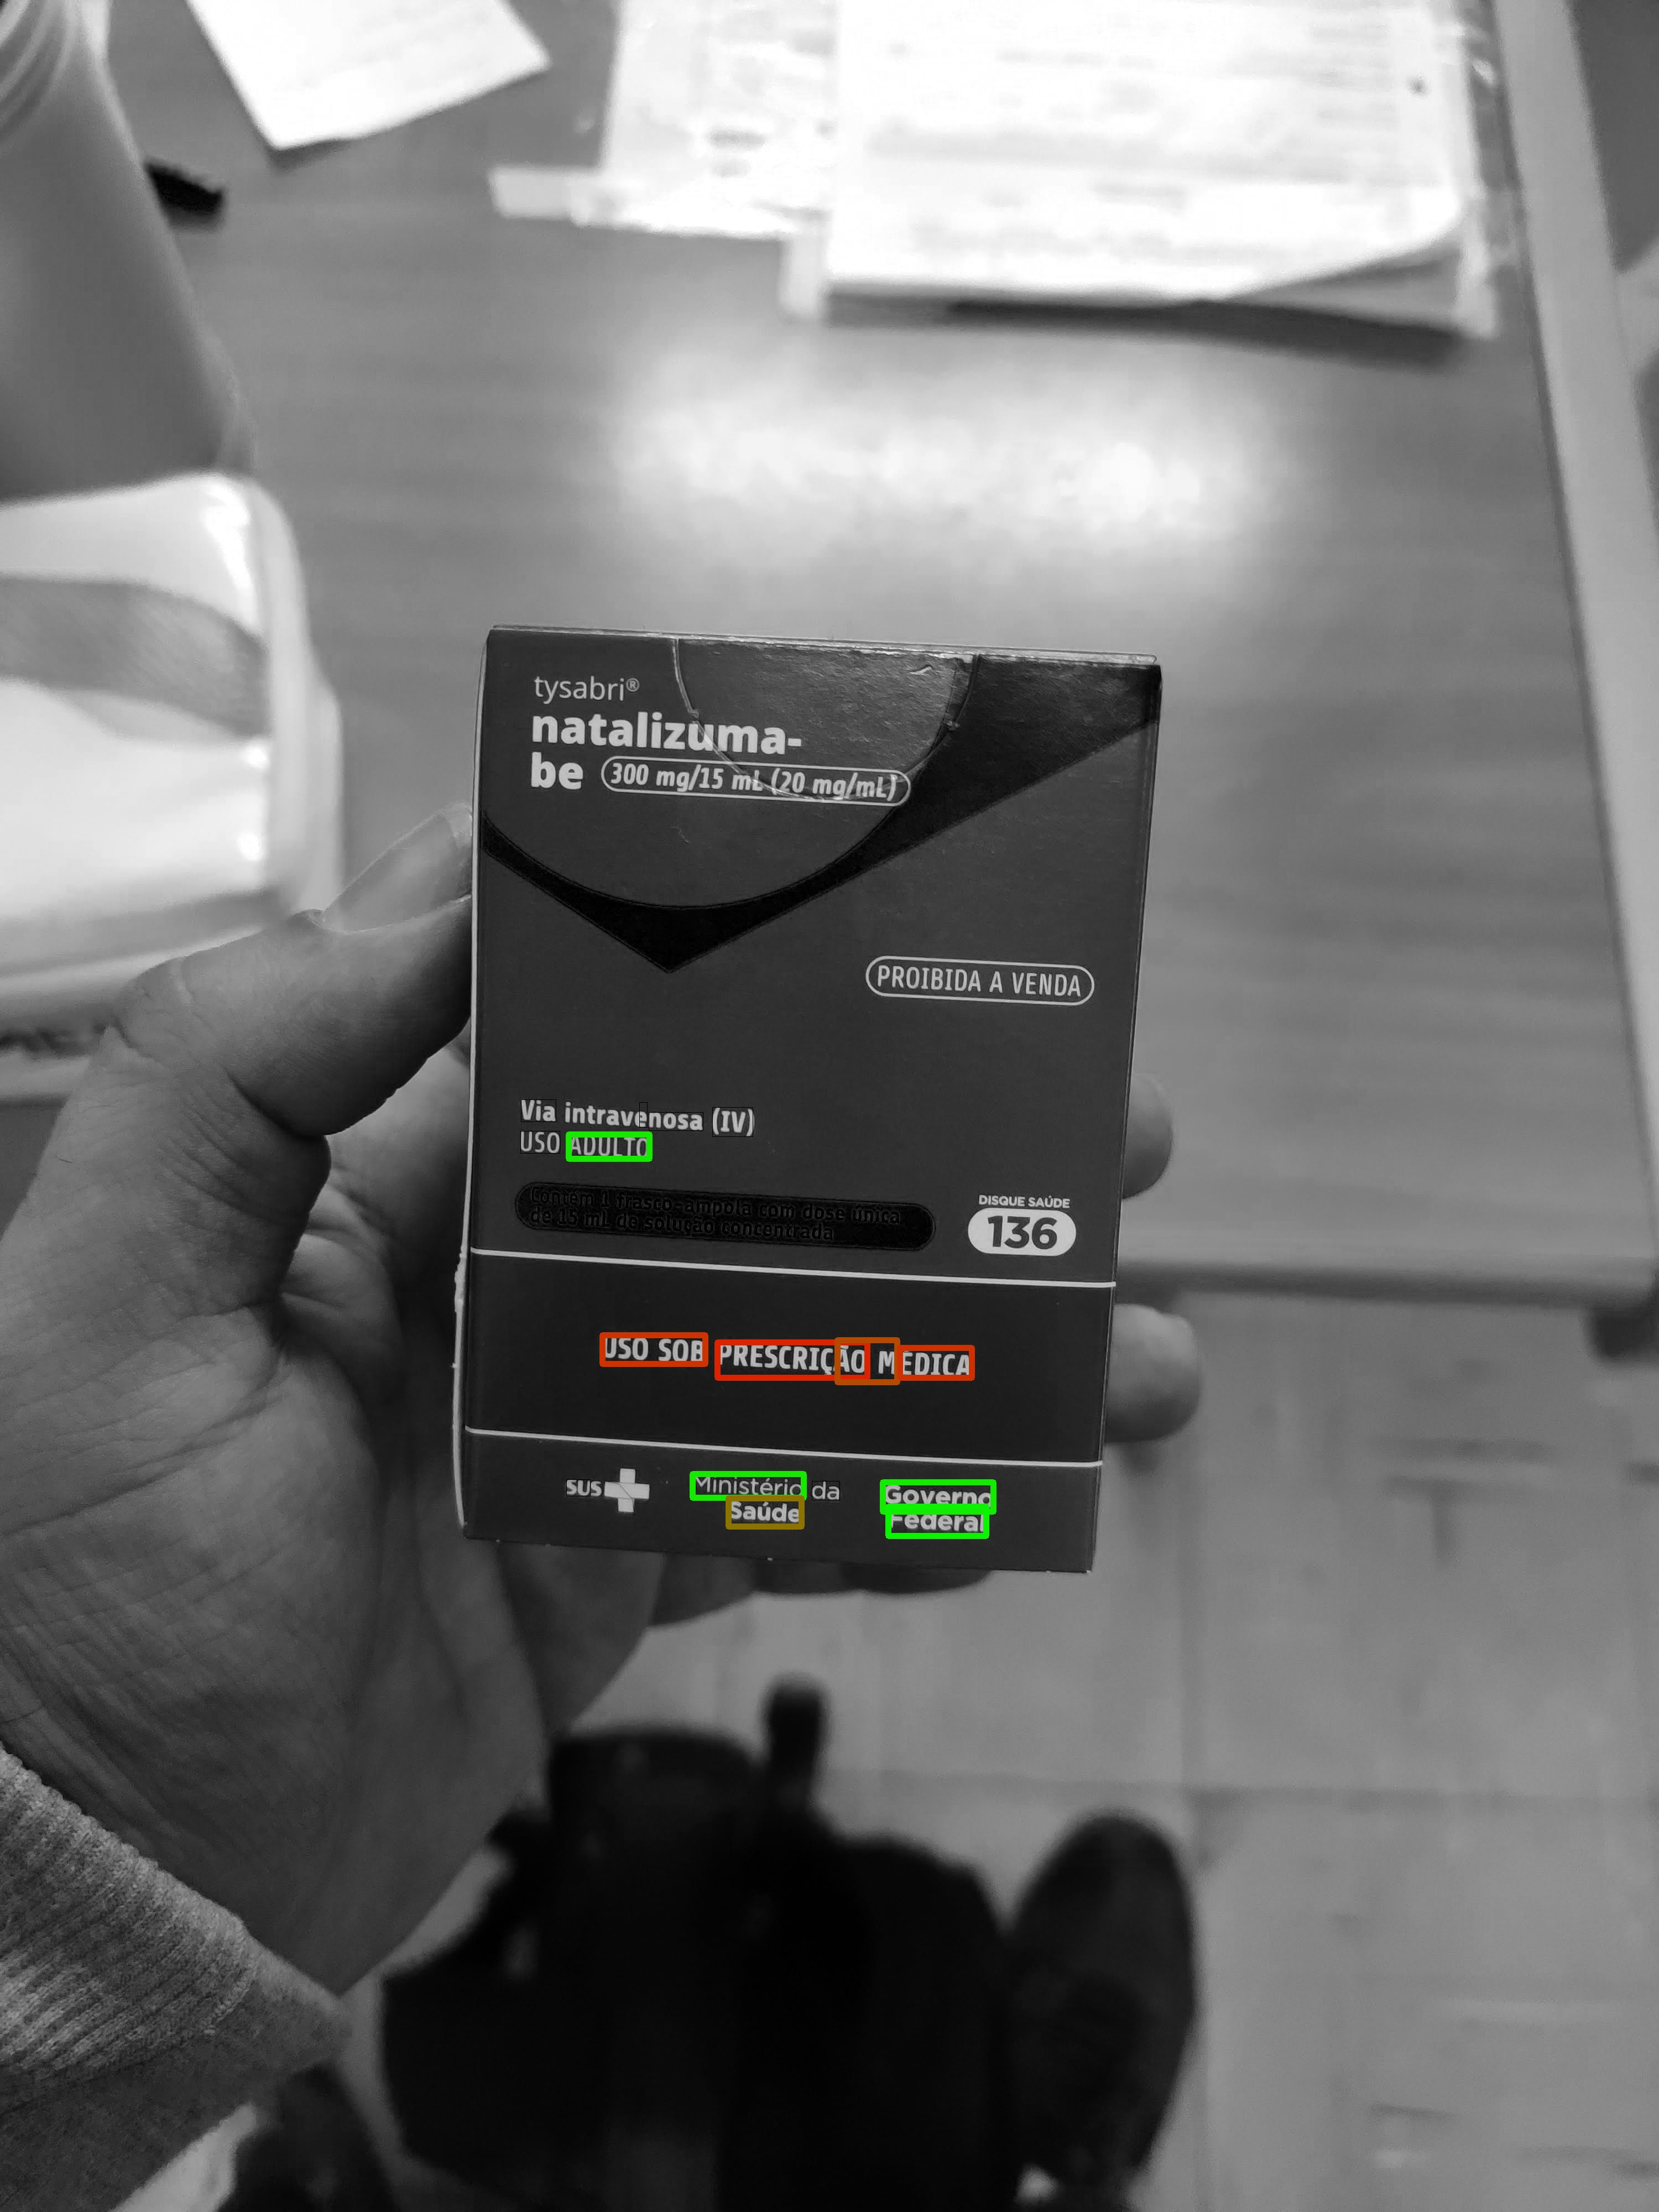
\includegraphics[width=\linewidth]{../pictures/tysabri_rgb_b_only_boxes.jpg}
    \end{subfigure}
    \\\vspace{\floatsep}
    \begin{subfigure}[t]{0.21\textwidth}
        \centering
        \caption{Cinza thresh.}
        \label{fig:foto:versoes:1:Cinza_thresh}
        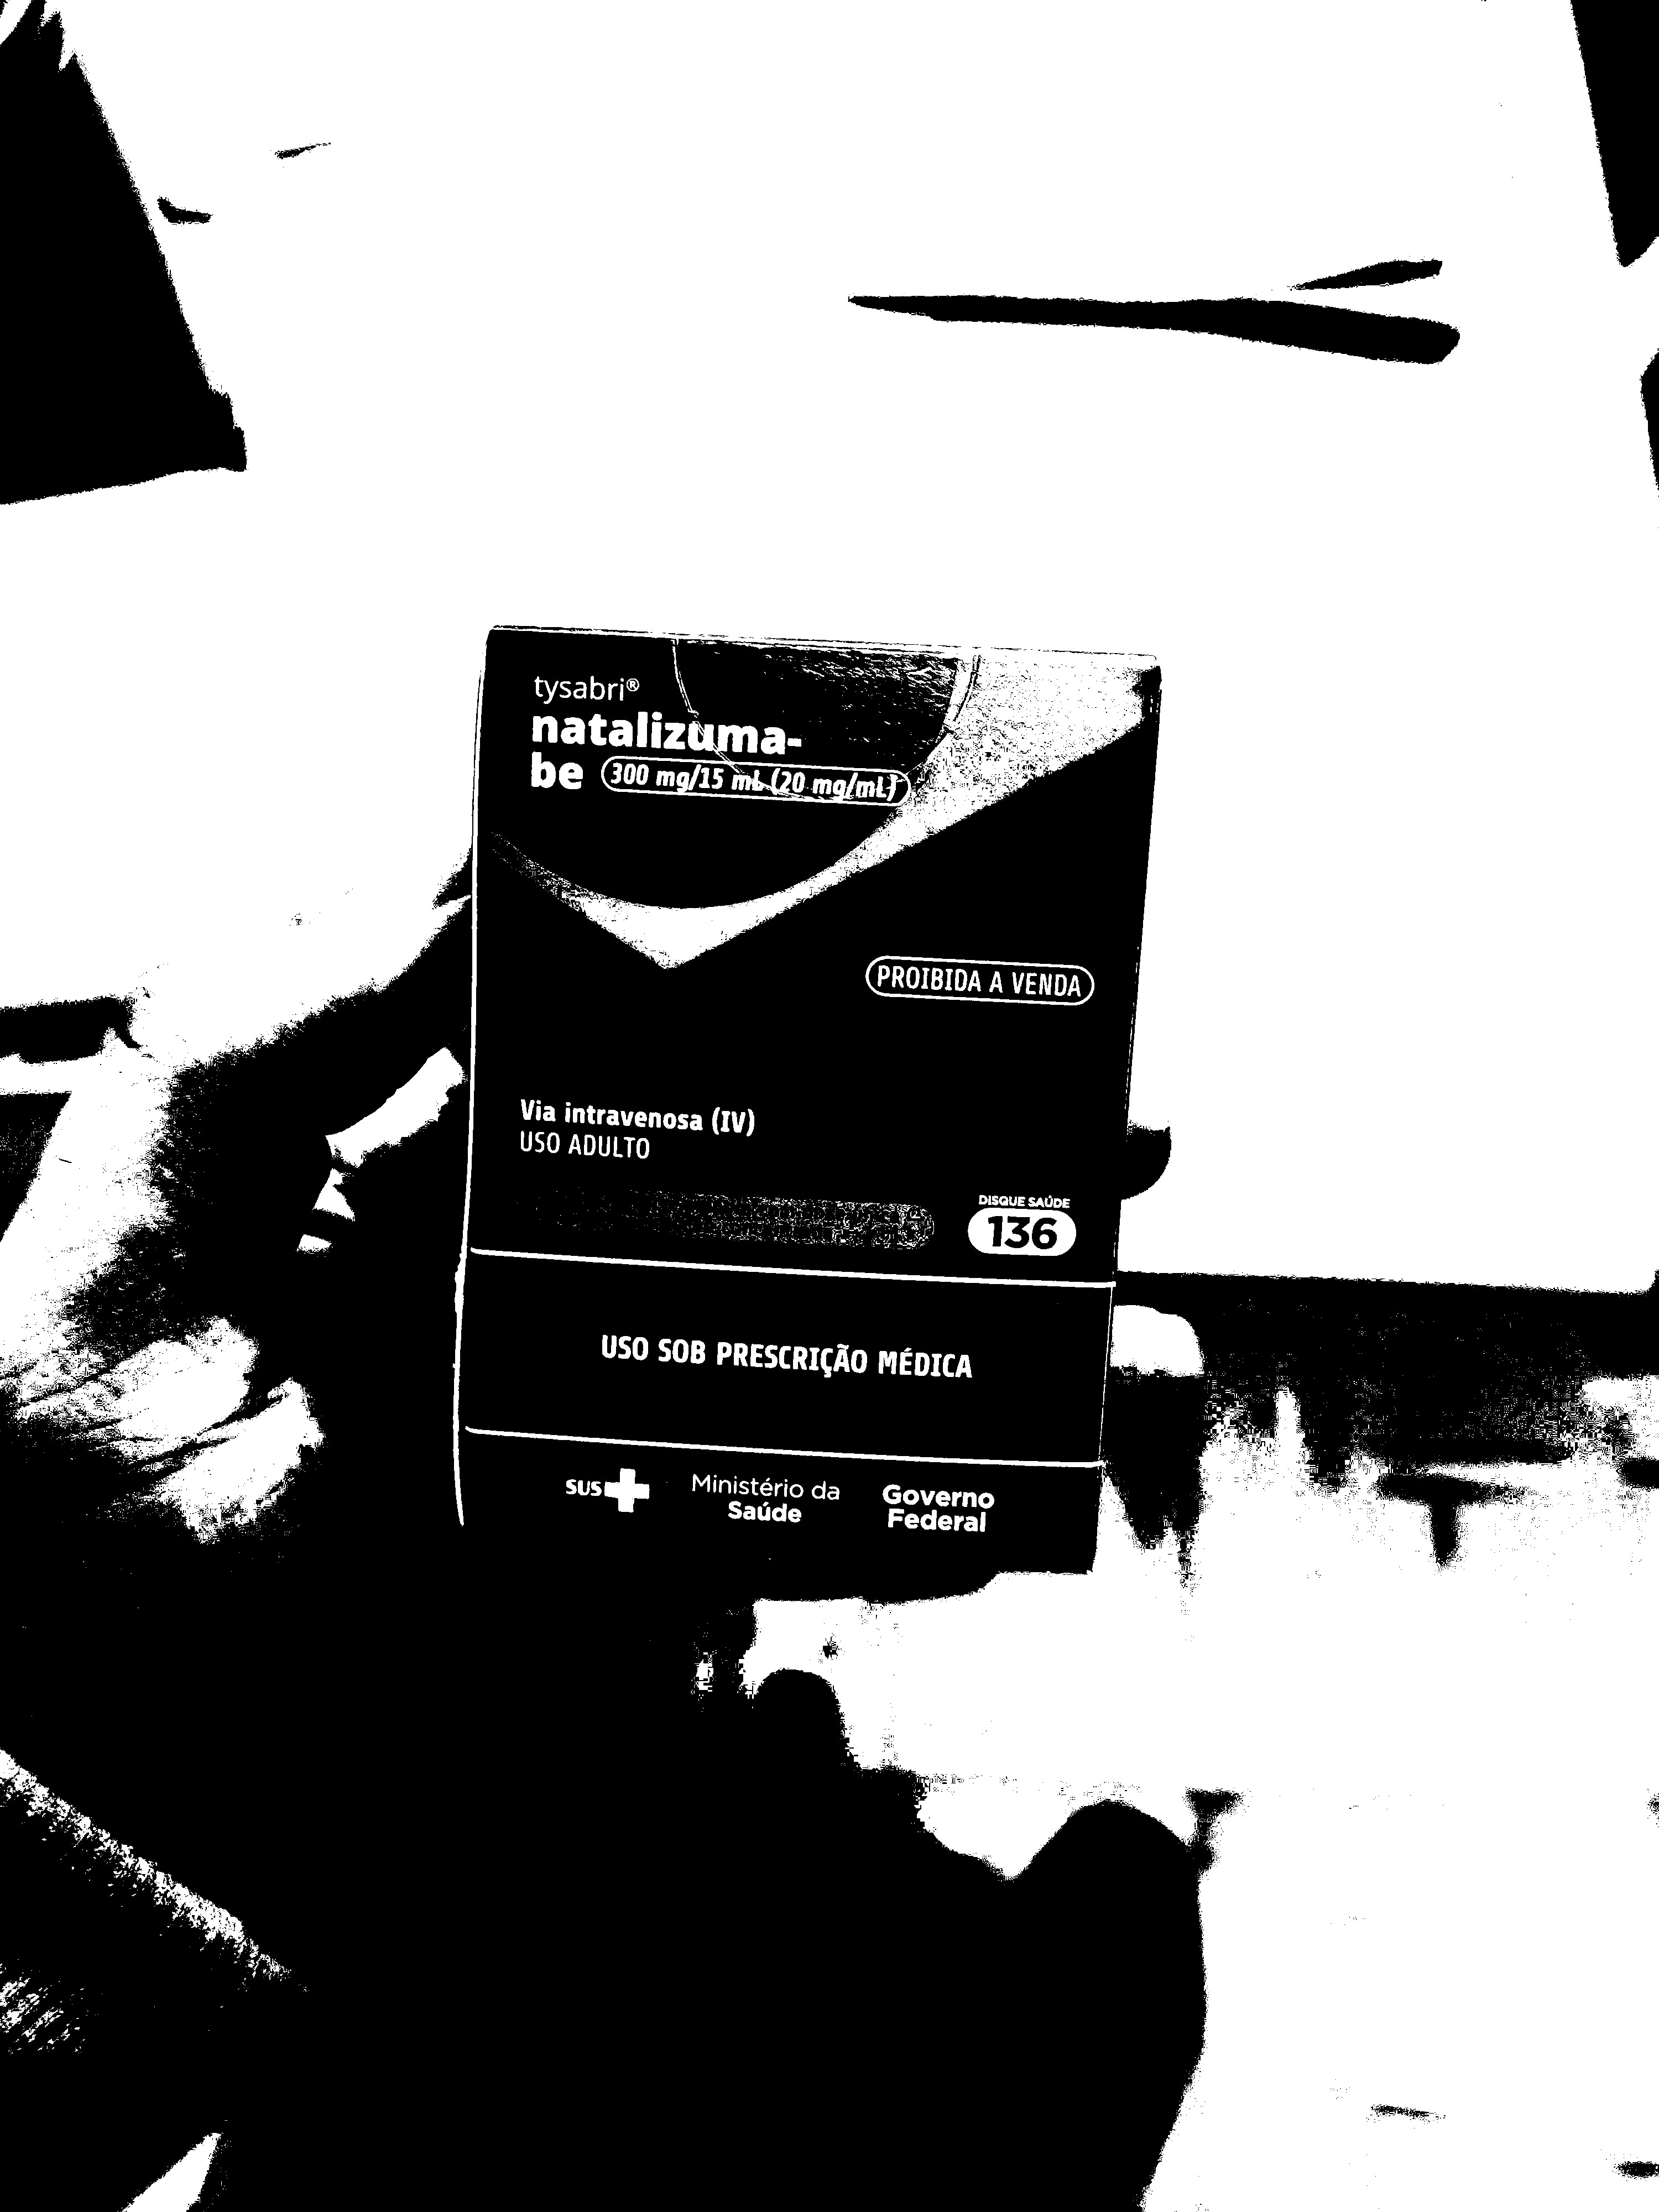
\includegraphics[width=\linewidth]{../pictures/tysabri_gray_thresh.jpg}
    \end{subfigure}
    \hfill
    \begin{subfigure}[t]{0.21\textwidth}
        \centering
        \caption{R thresh.}
        \label{fig:foto:versoes:1:R_thresh}
        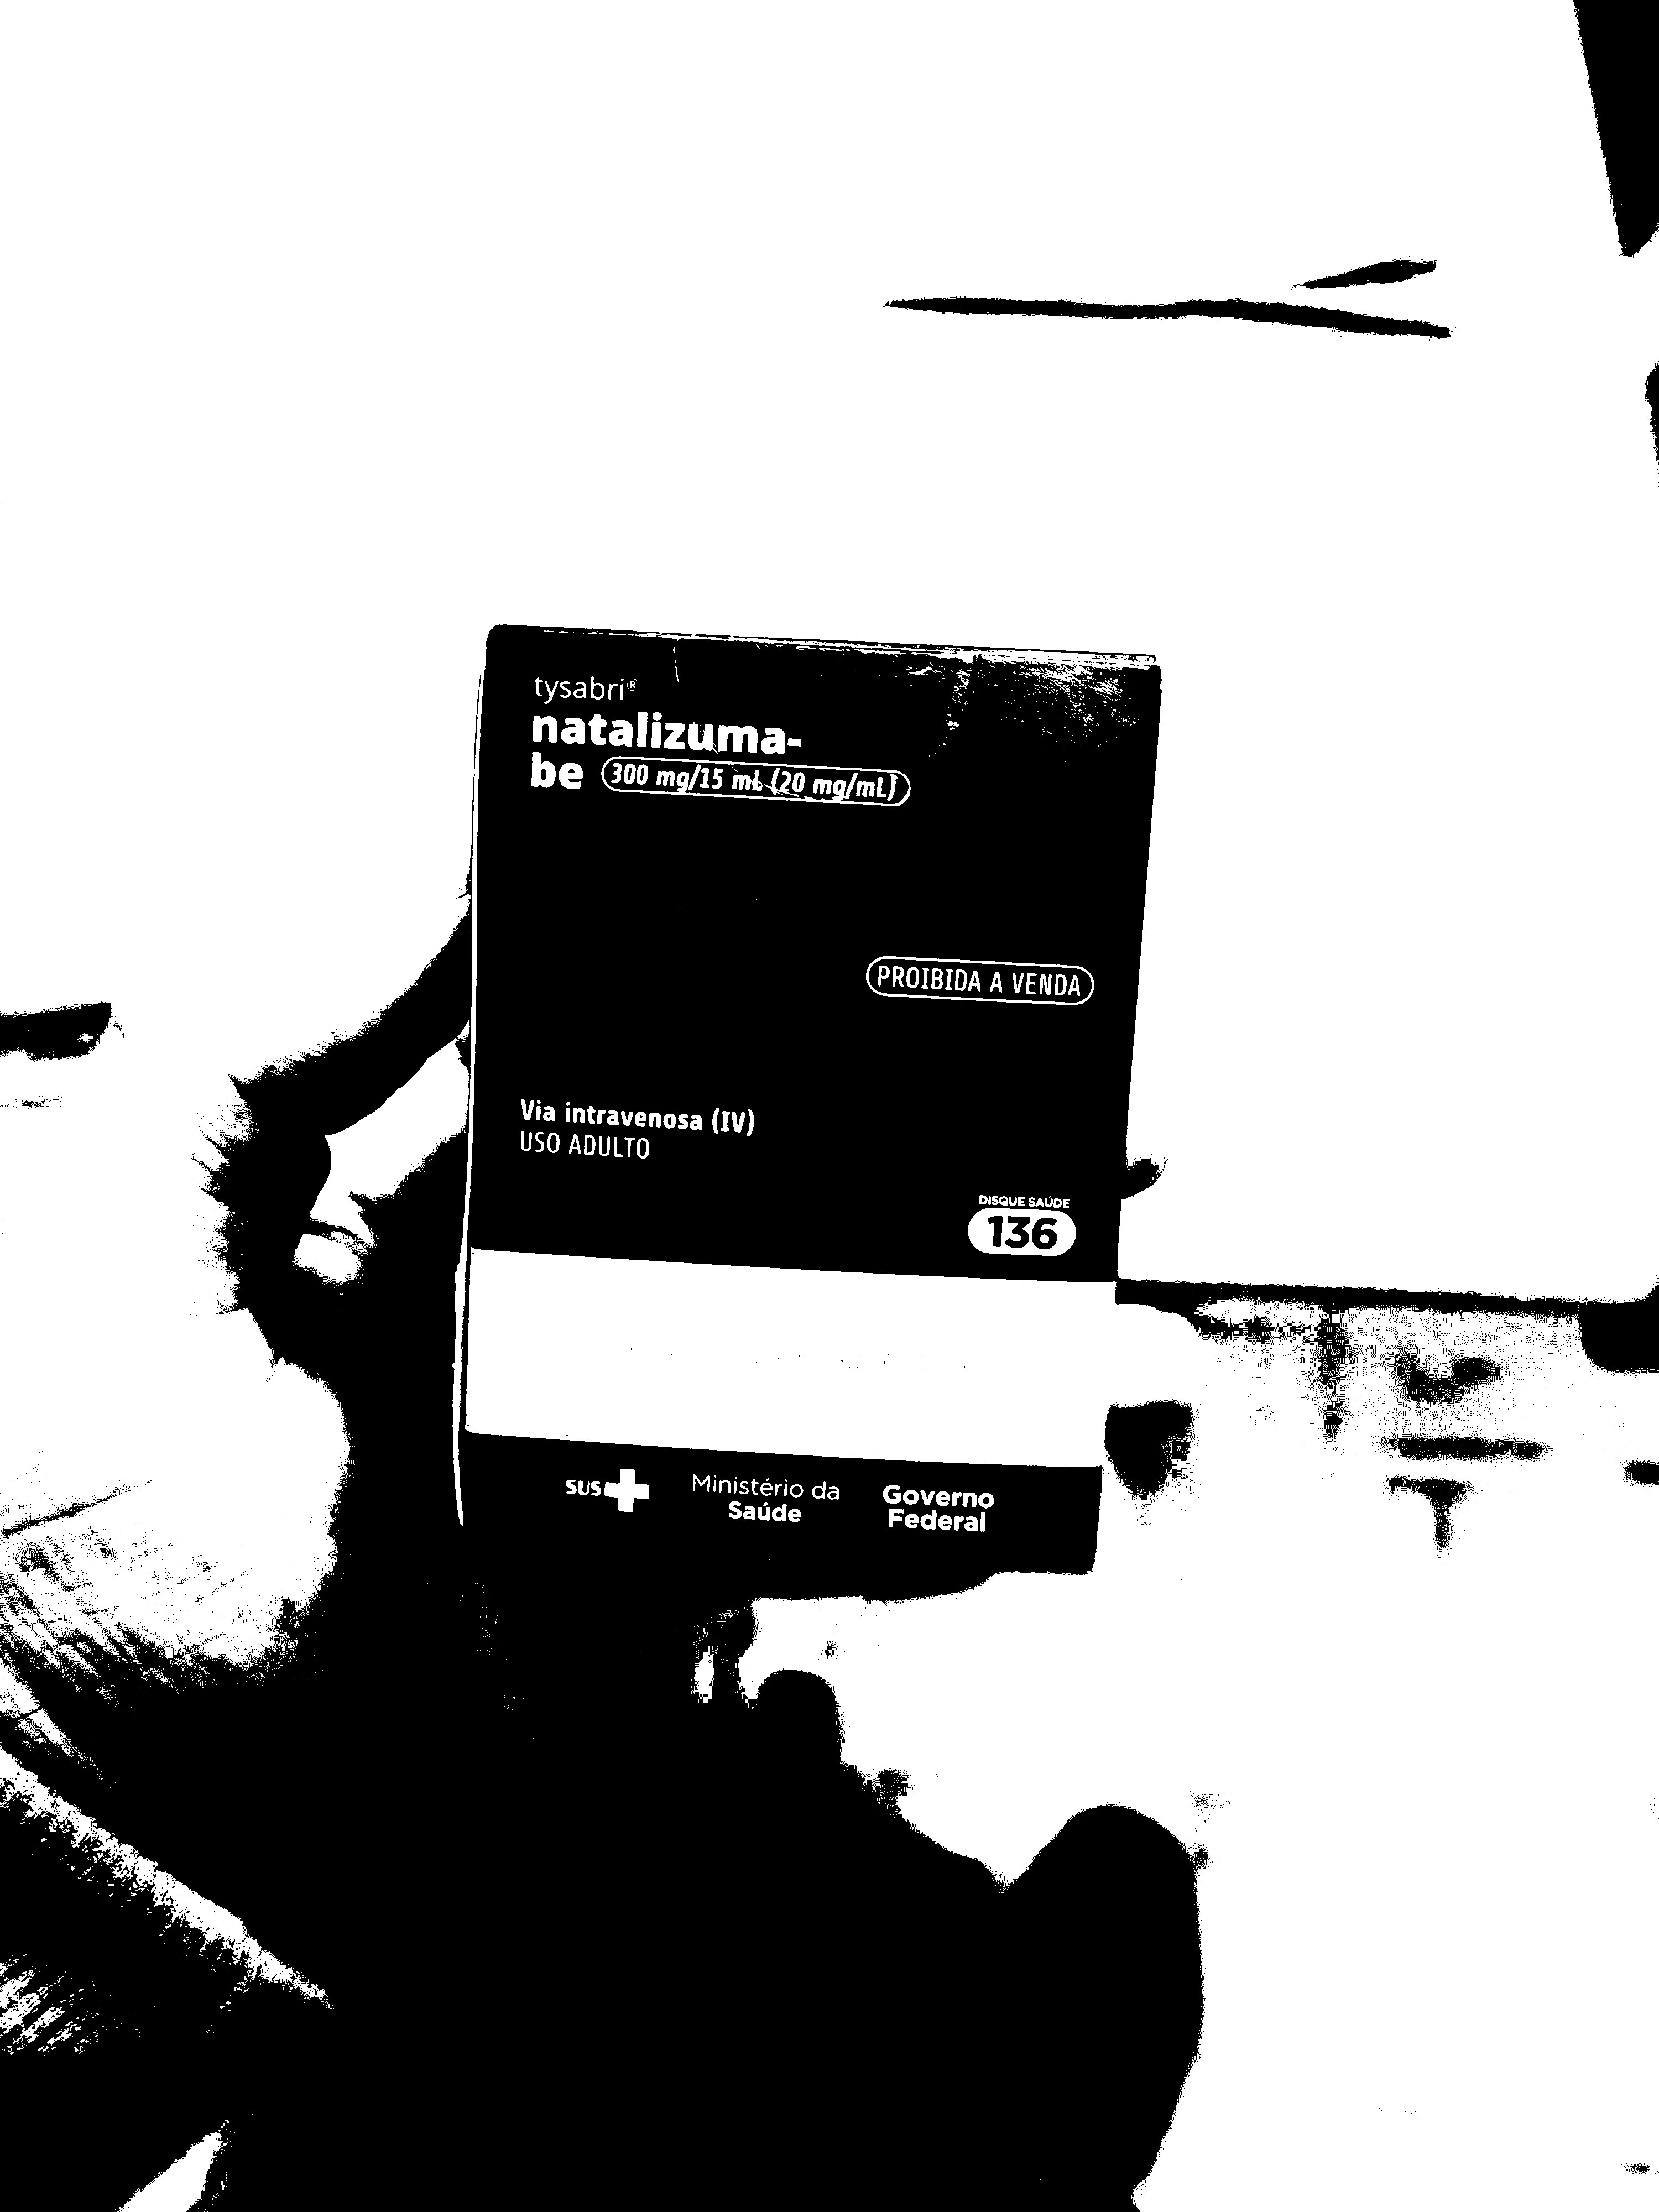
\includegraphics[width=\linewidth]{../pictures/tysabri_rgb_r_only_thresh.jpg}
    \end{subfigure}
    \hfill
    \begin{subfigure}[t]{0.21\textwidth}
        \centering
        \caption{G thresh.}
        \label{fig:foto:versoes:1:G_thresh}
        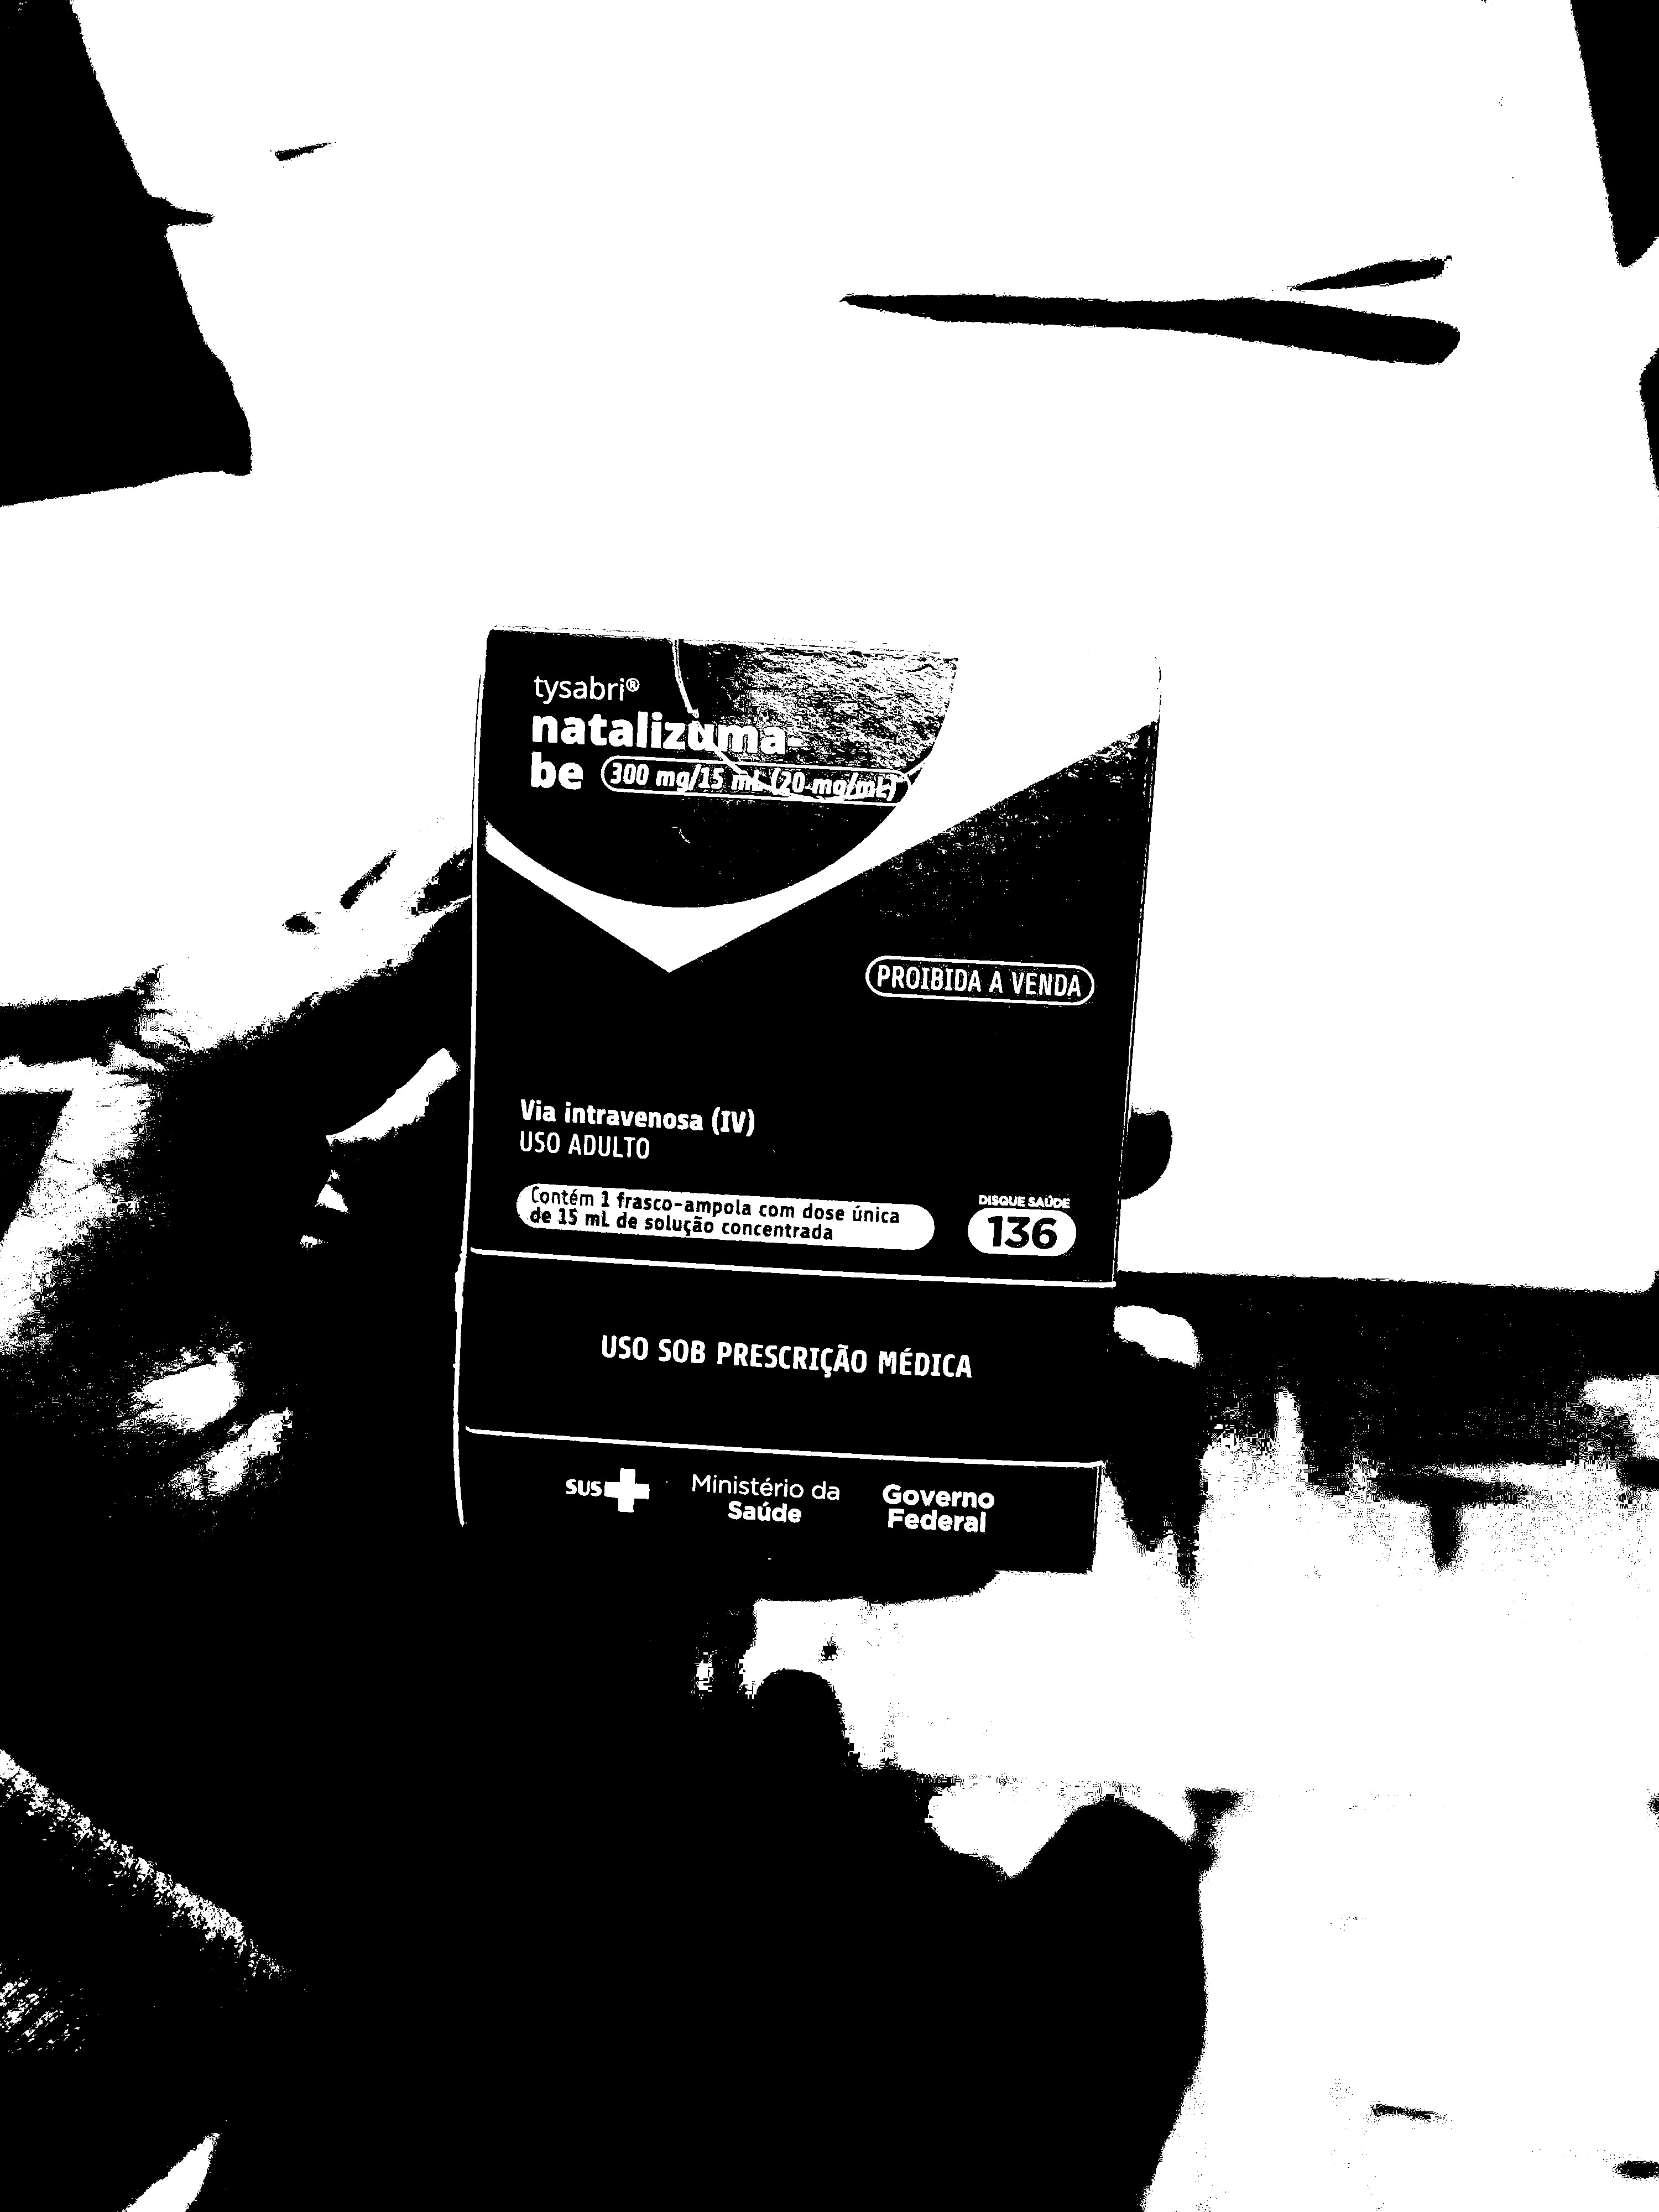
\includegraphics[width=\linewidth]{../pictures/tysabri_rgb_g_only_thresh.jpg}
    \end{subfigure}
    \hfill
    \begin{subfigure}[t]{0.21\textwidth}
        \centering
        \caption{B thresh.}
        \label{fig:foto:versoes:1:B_thresh}
        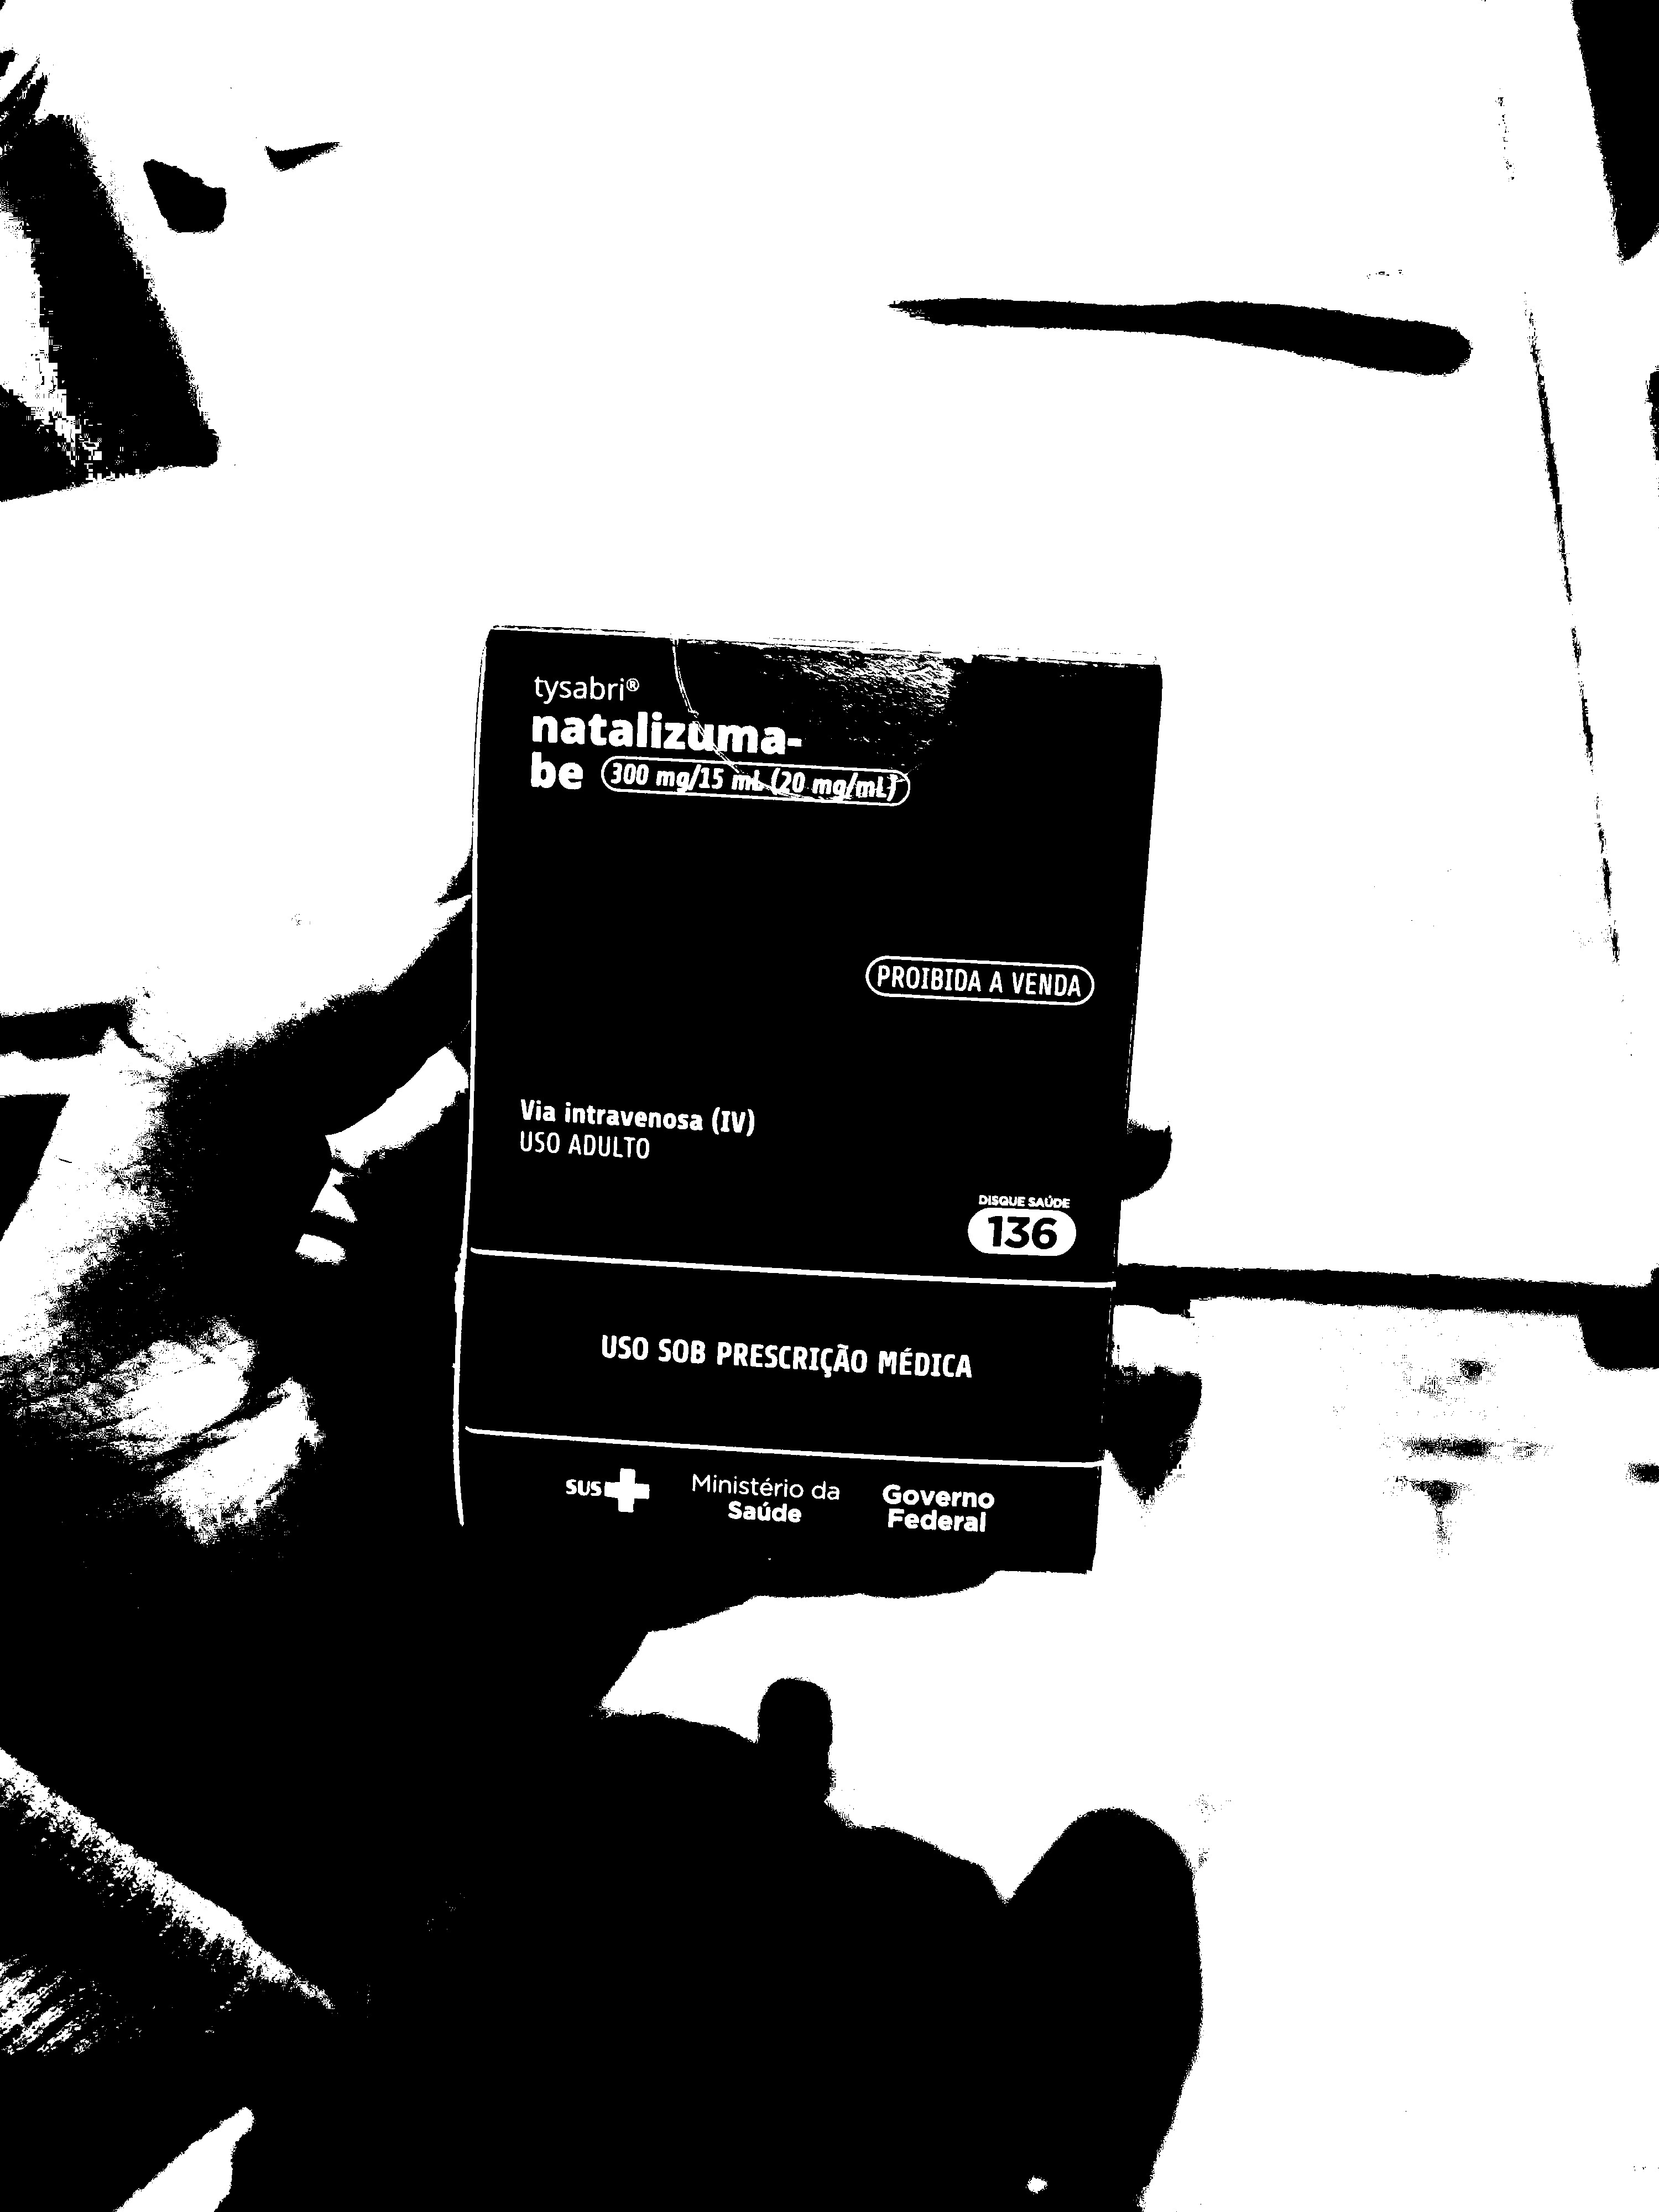
\includegraphics[width=\linewidth]{../pictures/tysabri_rgb_b_only_thresh.jpg}
    \end{subfigure}
    \\\vspace{\floatsep}
    \begin{subfigure}[t]{0.21\textwidth}
        \centering
        \caption{Cinza thresh.}
        \label{fig:foto:versoes:1:Cinza_thresh:boxes}
        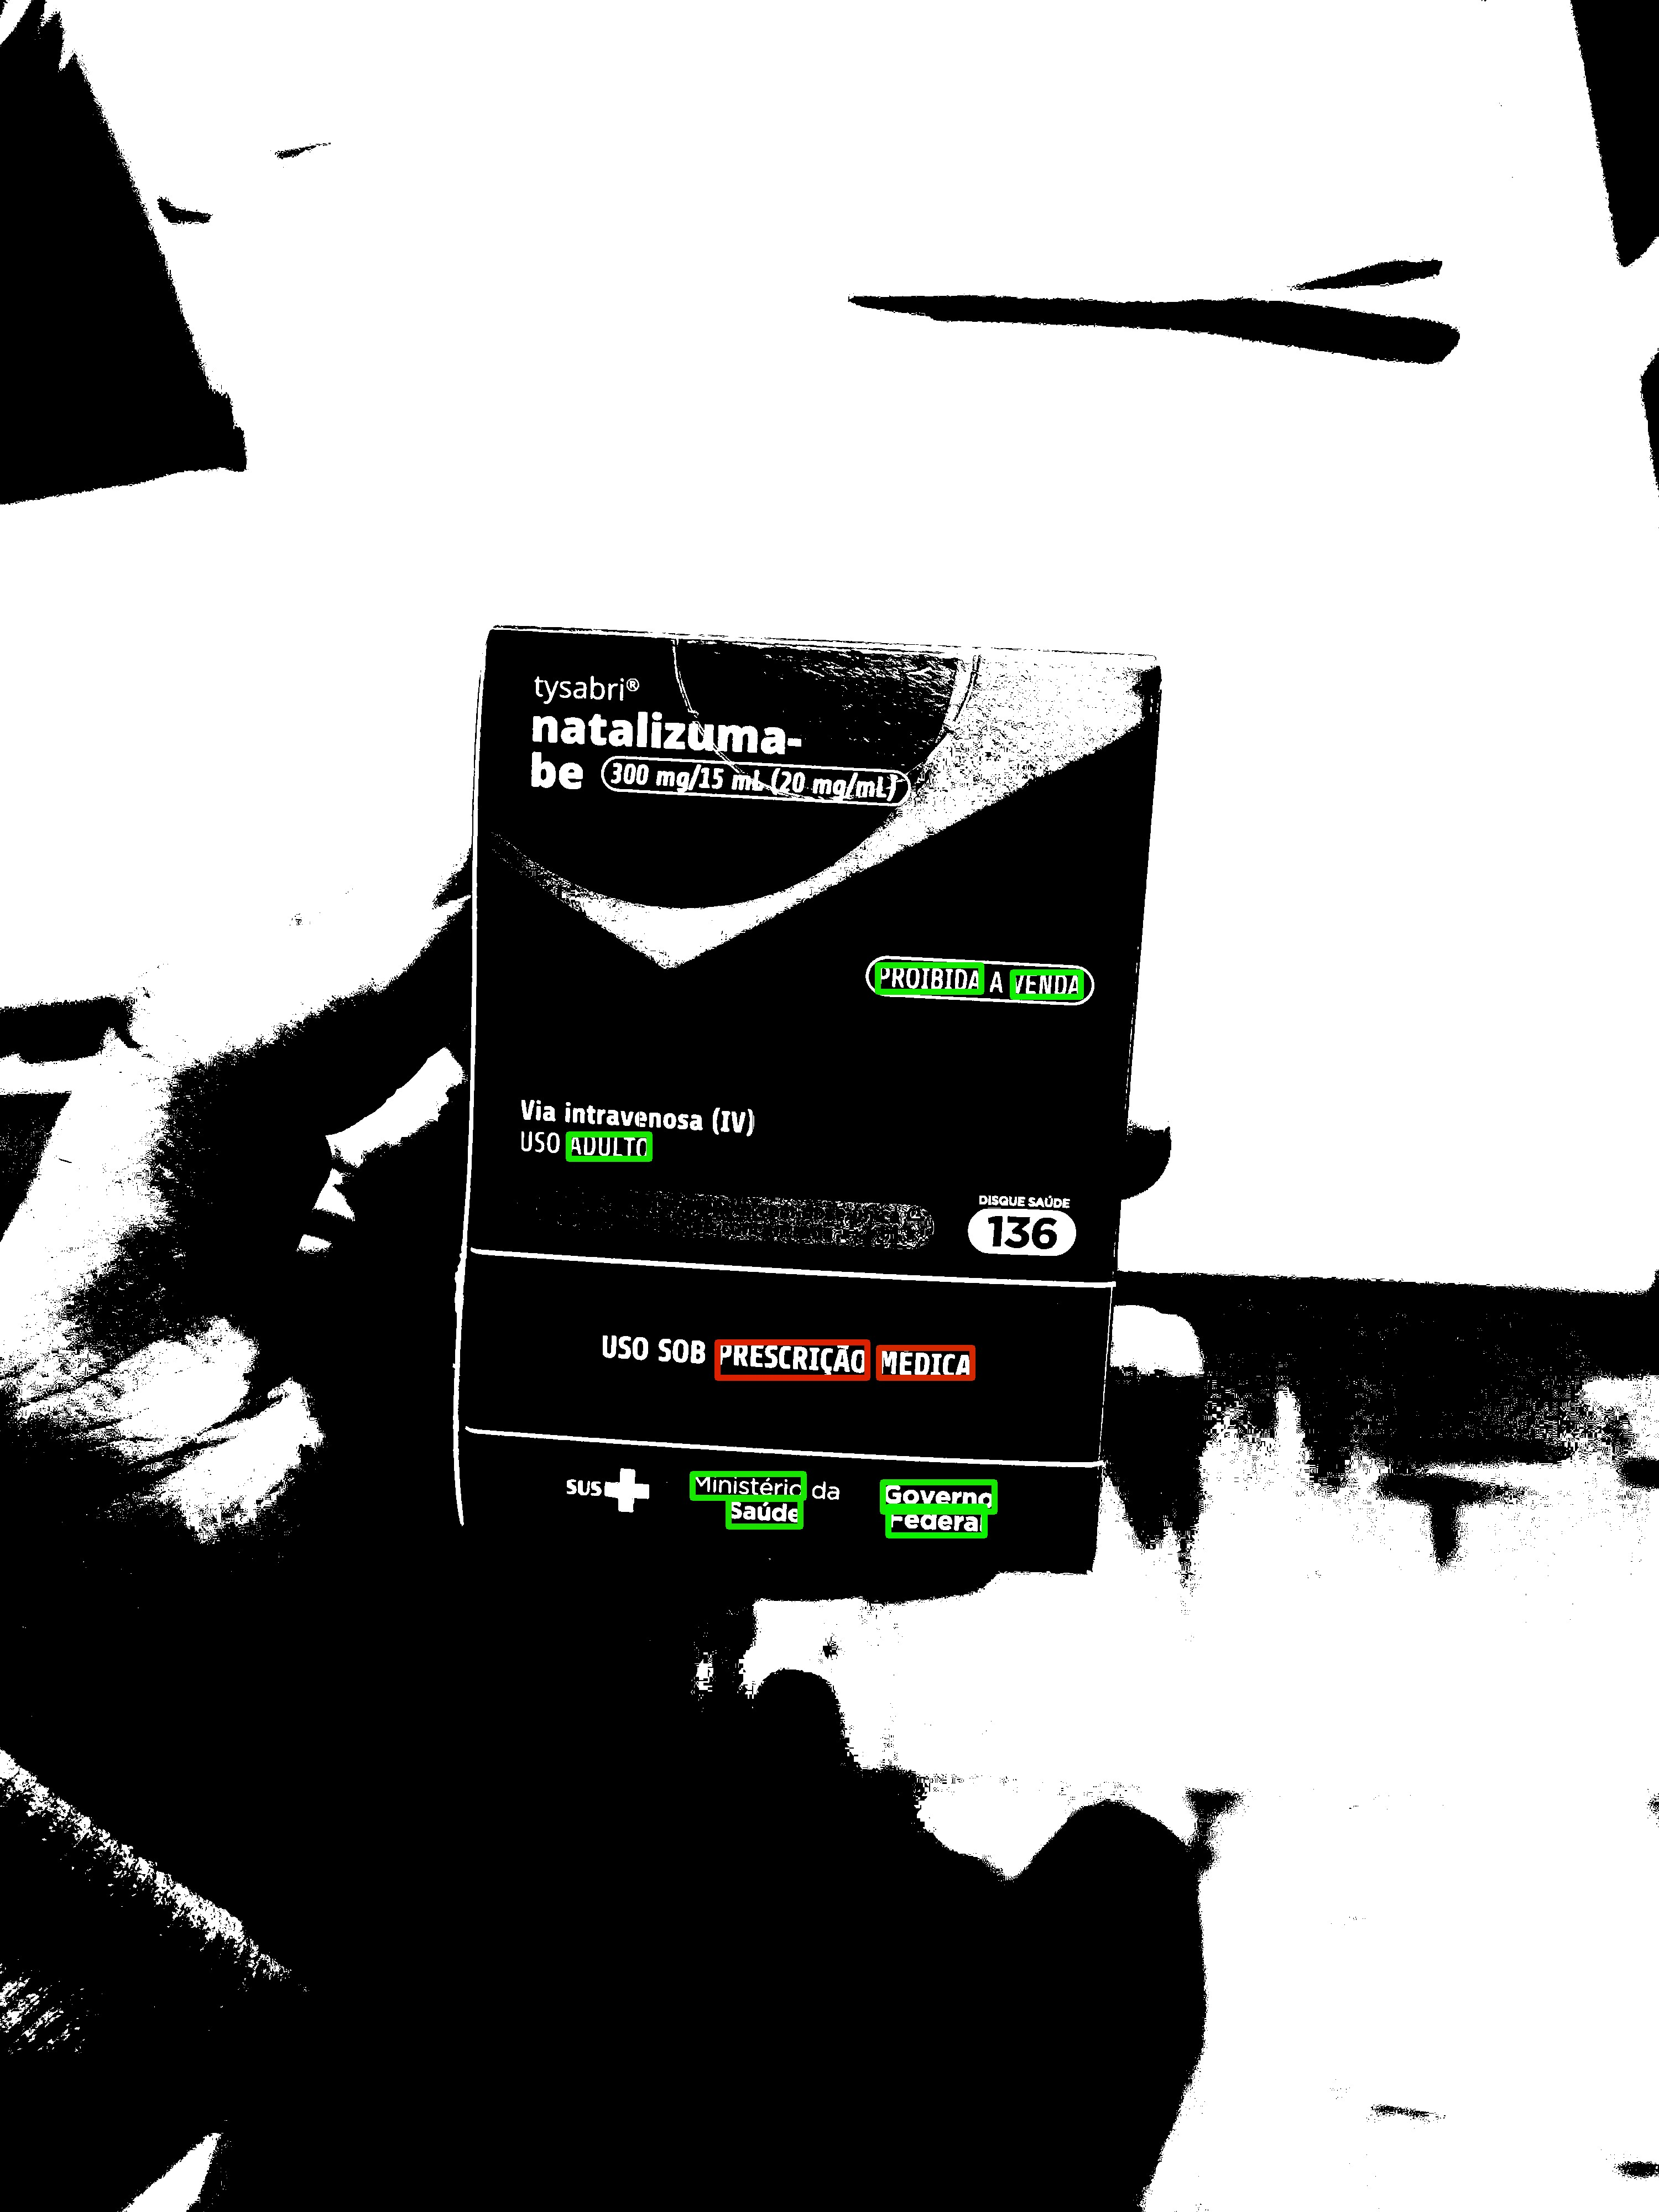
\includegraphics[width=\linewidth]{../pictures/tysabri_gray_thresh_boxes.jpg}
    \end{subfigure}
    \hfill
    \begin{subfigure}[t]{0.21\textwidth}
        \centering
        \caption{R thresh.}
        \label{fig:foto:versoes:1:R_thresh:boxes}
        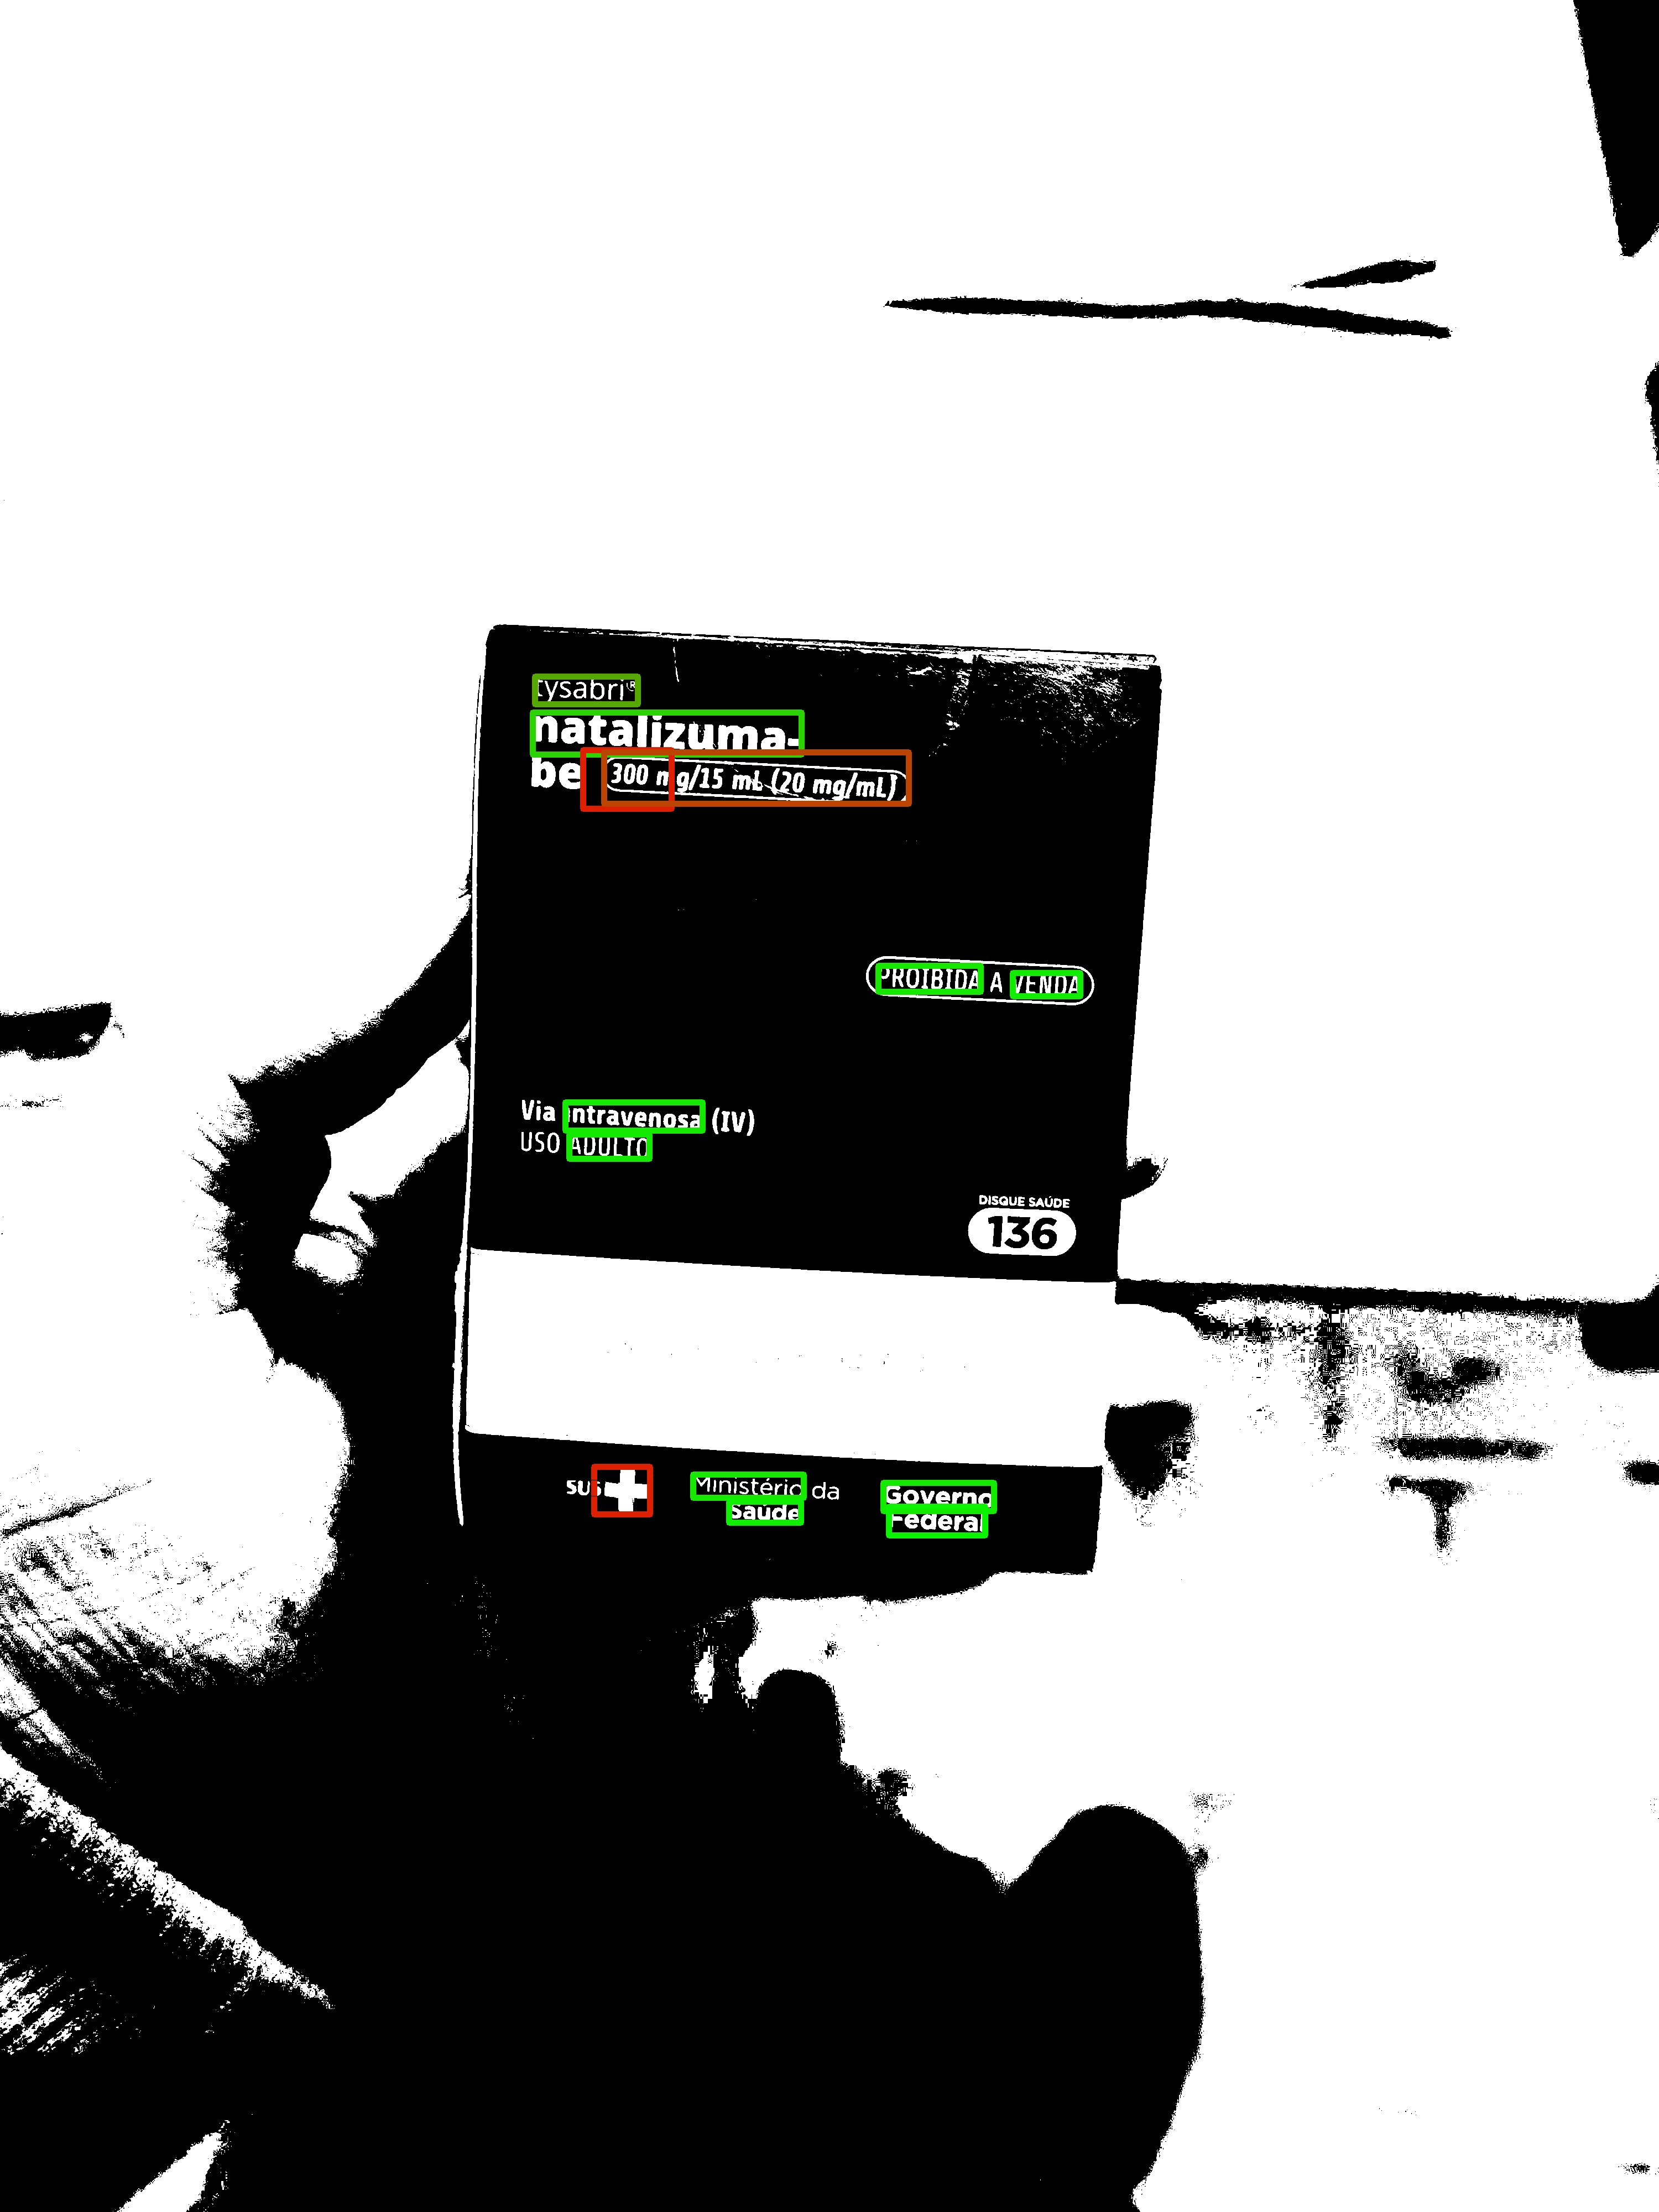
\includegraphics[width=\linewidth]{../pictures/tysabri_rgb_r_only_thresh_boxes.jpg}
    \end{subfigure}
    \hfill
    \begin{subfigure}[t]{0.21\textwidth}
        \centering
        \caption{G thresh.}
        \label{fig:foto:versoes:1:G_thresh:boxes}
        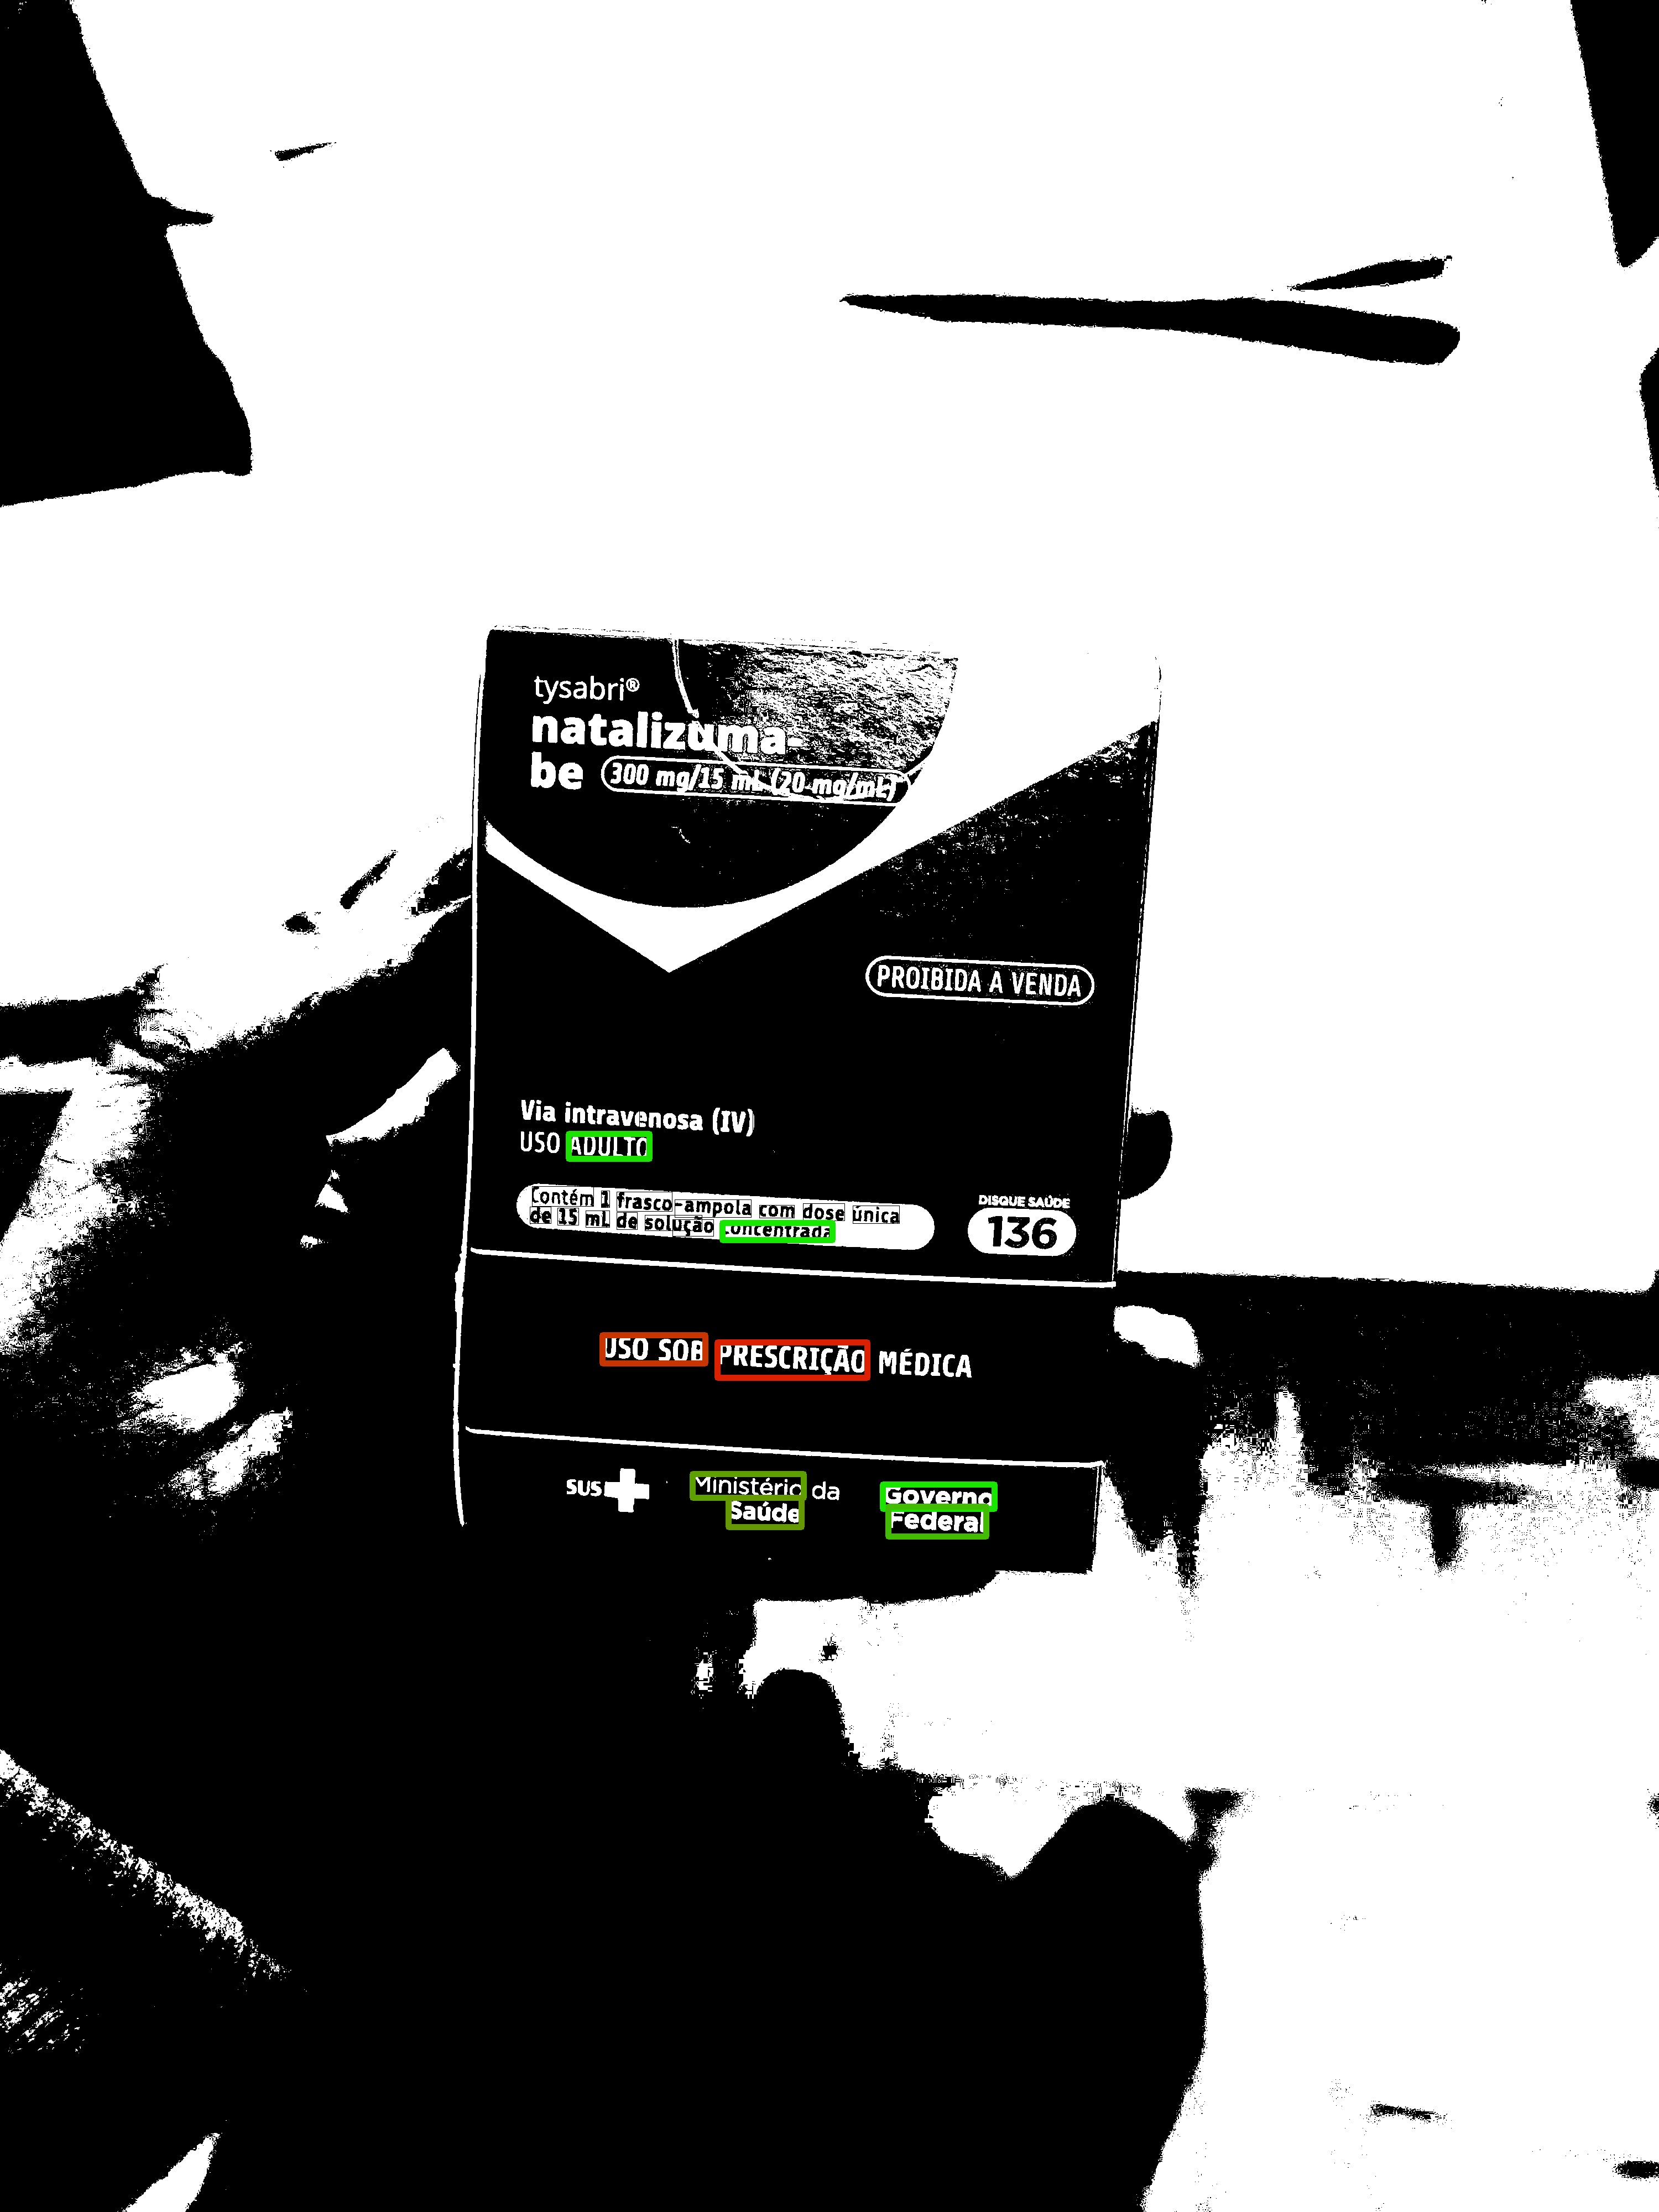
\includegraphics[width=\linewidth]{../pictures/tysabri_rgb_g_only_thresh_boxes.jpg}
    \end{subfigure}
    \hfill
    \begin{subfigure}[t]{0.21\textwidth}
        \centering
        \caption{B thresh.}
        \label{fig:foto:versoes:1:B_thresh:boxes}
        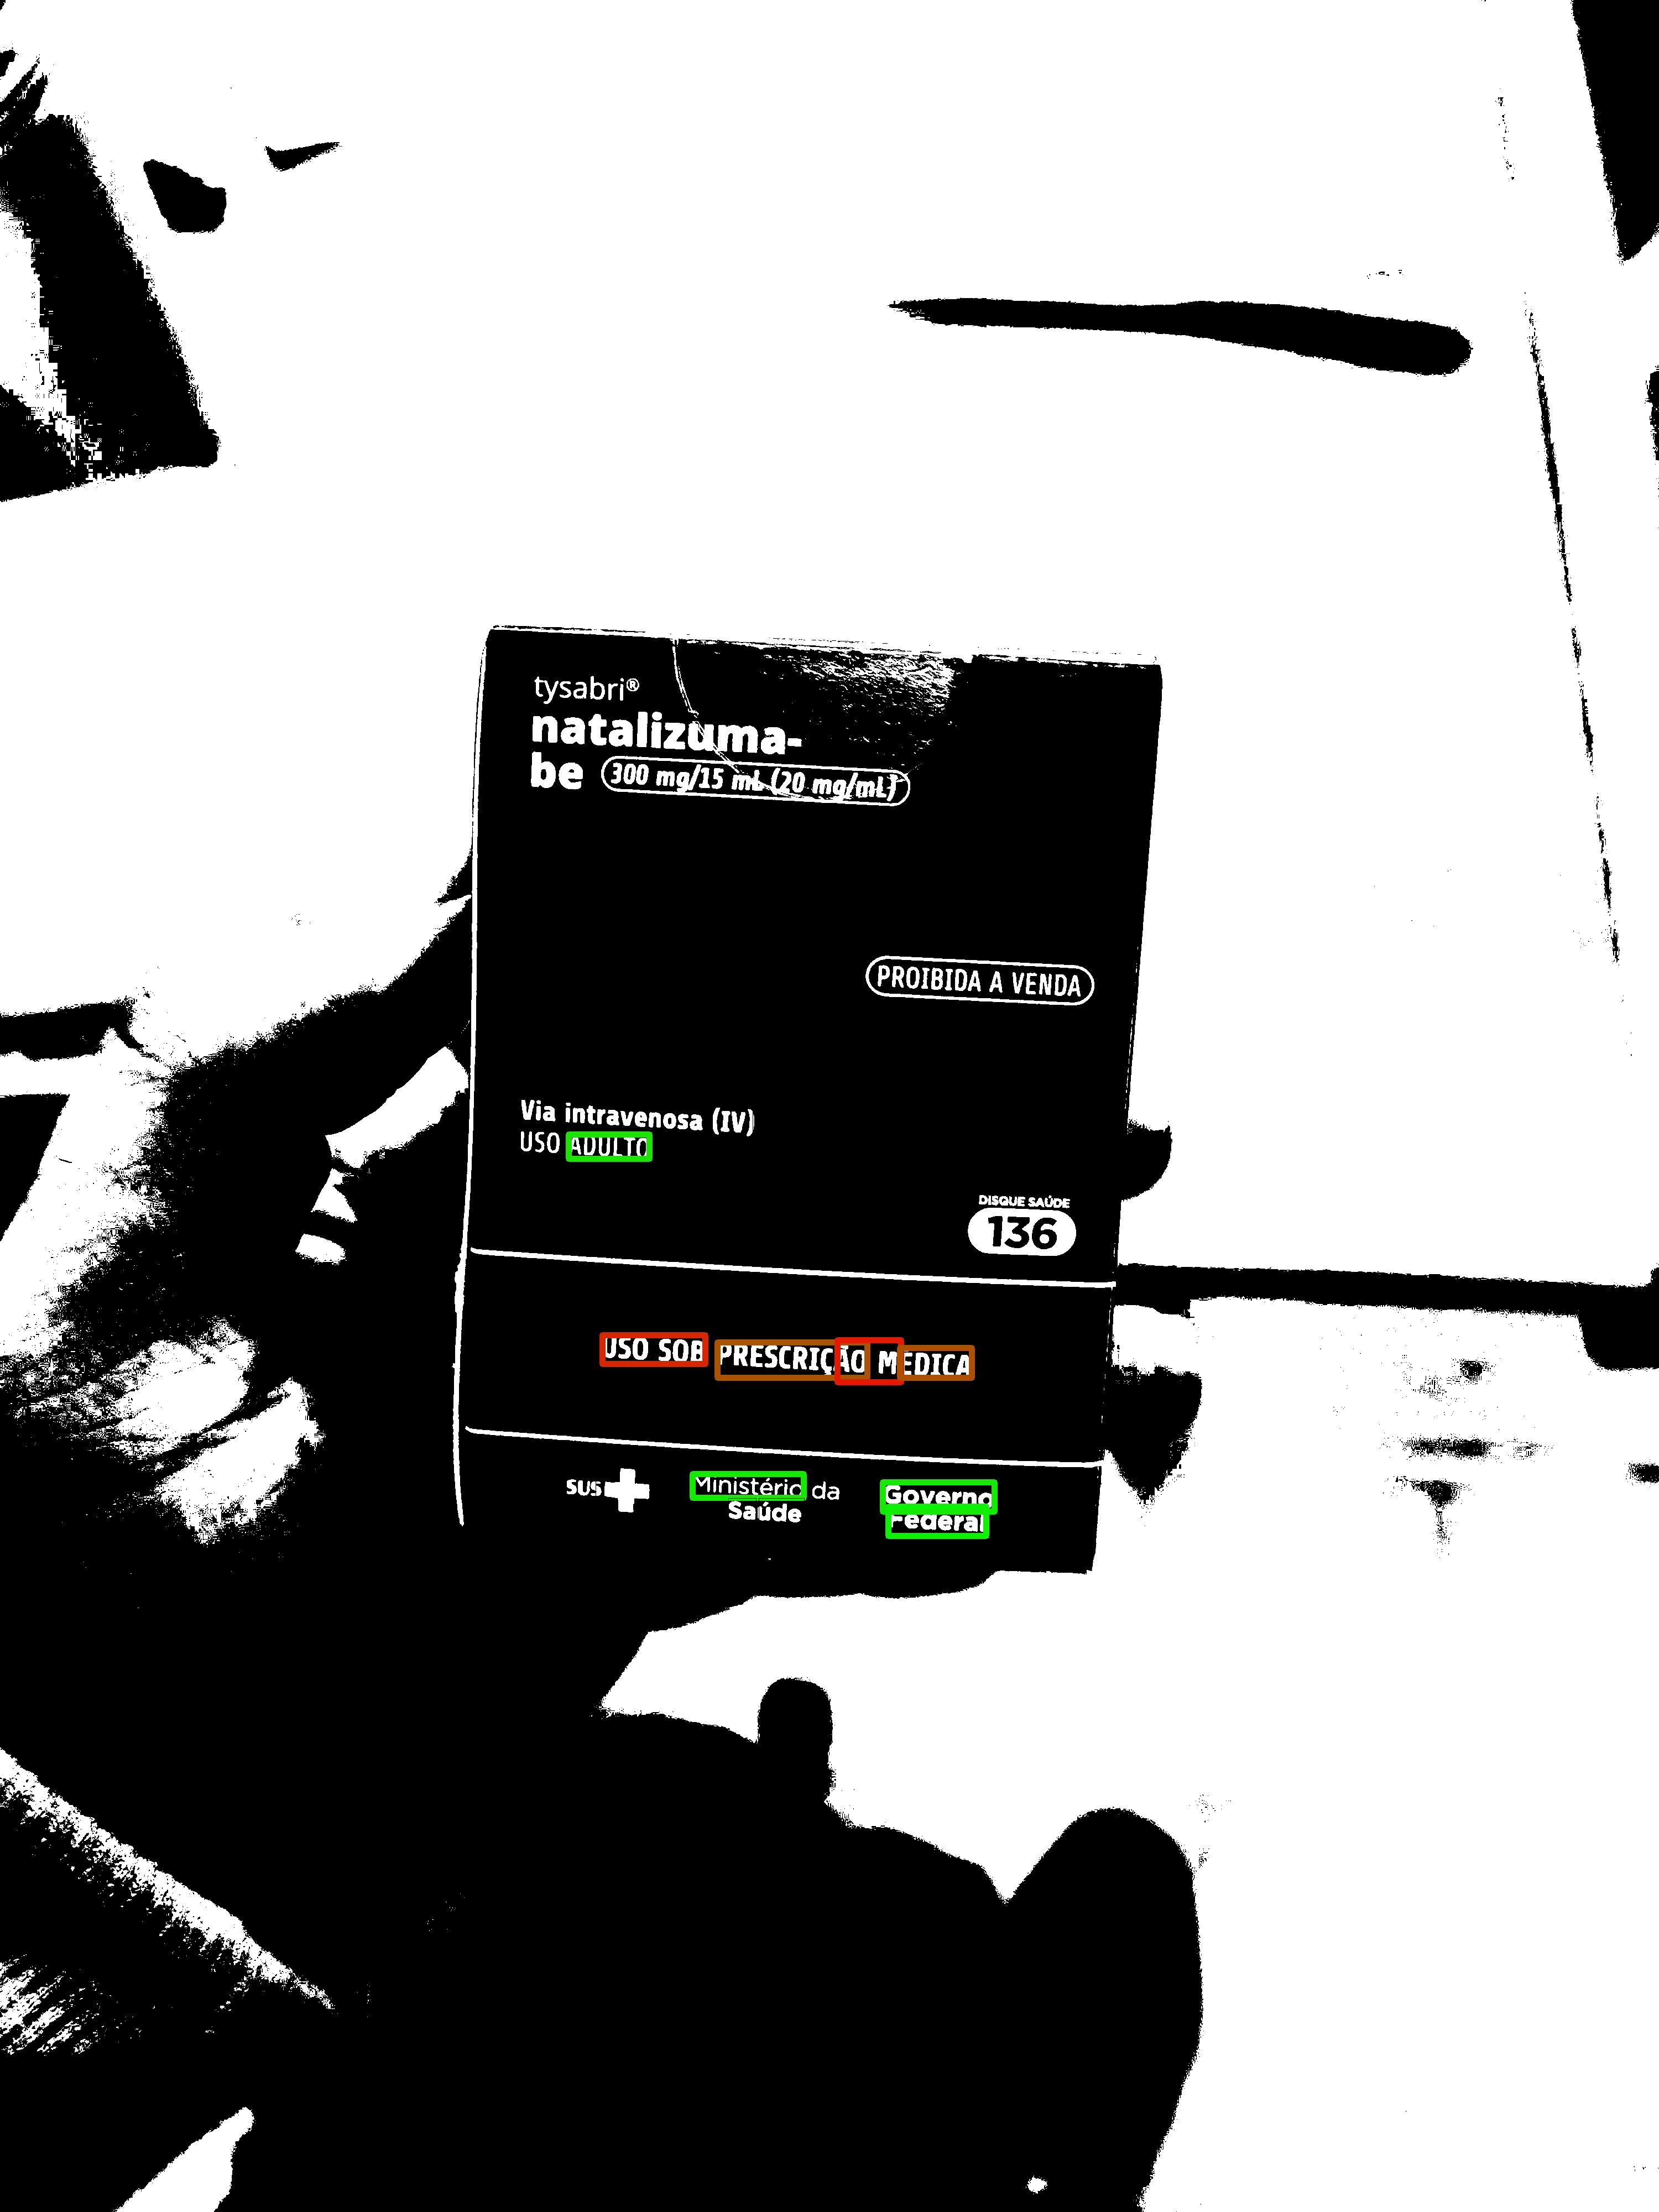
\includegraphics[width=\linewidth]{../pictures/tysabri_rgb_b_only_thresh_boxes.jpg}
    \end{subfigure}
    \caption*{Fonte: Autor.}
    \label{fig:foto:versoes:1}
\end{figure}


\begin{figure}[htb]
    \centering
    \caption{Exemplos de componentes analisadas CMYK (%
    \subref{fig:foto:versoes:2:C},
    \subref{fig:foto:versoes:2:M},
    \subref{fig:foto:versoes:2:Y},
    \subref{fig:foto:versoes:2:K},
    \subref{fig:foto:versoes:2:C_thresh},
    \subref{fig:foto:versoes:2:M_thresh},
    \subref{fig:foto:versoes:2:Y_thresh},
    \subref{fig:foto:versoes:2:K_thresh}%
    ) e destaque nos termos localizados em cada componente (%
    \subref{fig:foto:versoes:2:C:boxes},
    \subref{fig:foto:versoes:2:M:boxes},
    \subref{fig:foto:versoes:2:Y:boxes},
    \subref{fig:foto:versoes:2:K:boxes},
    \subref{fig:foto:versoes:2:C_thresh:boxes},
    \subref{fig:foto:versoes:2:M_thresh:boxes},
    \subref{fig:foto:versoes:2:Y_thresh:boxes},
    \subref{fig:foto:versoes:2:K_thresh:boxes}%
    ).}
    % \hfill
    \begin{subfigure}[t]{0.21\textwidth}
        \centering
        \caption{C.}
        \label{fig:foto:versoes:2:C}
        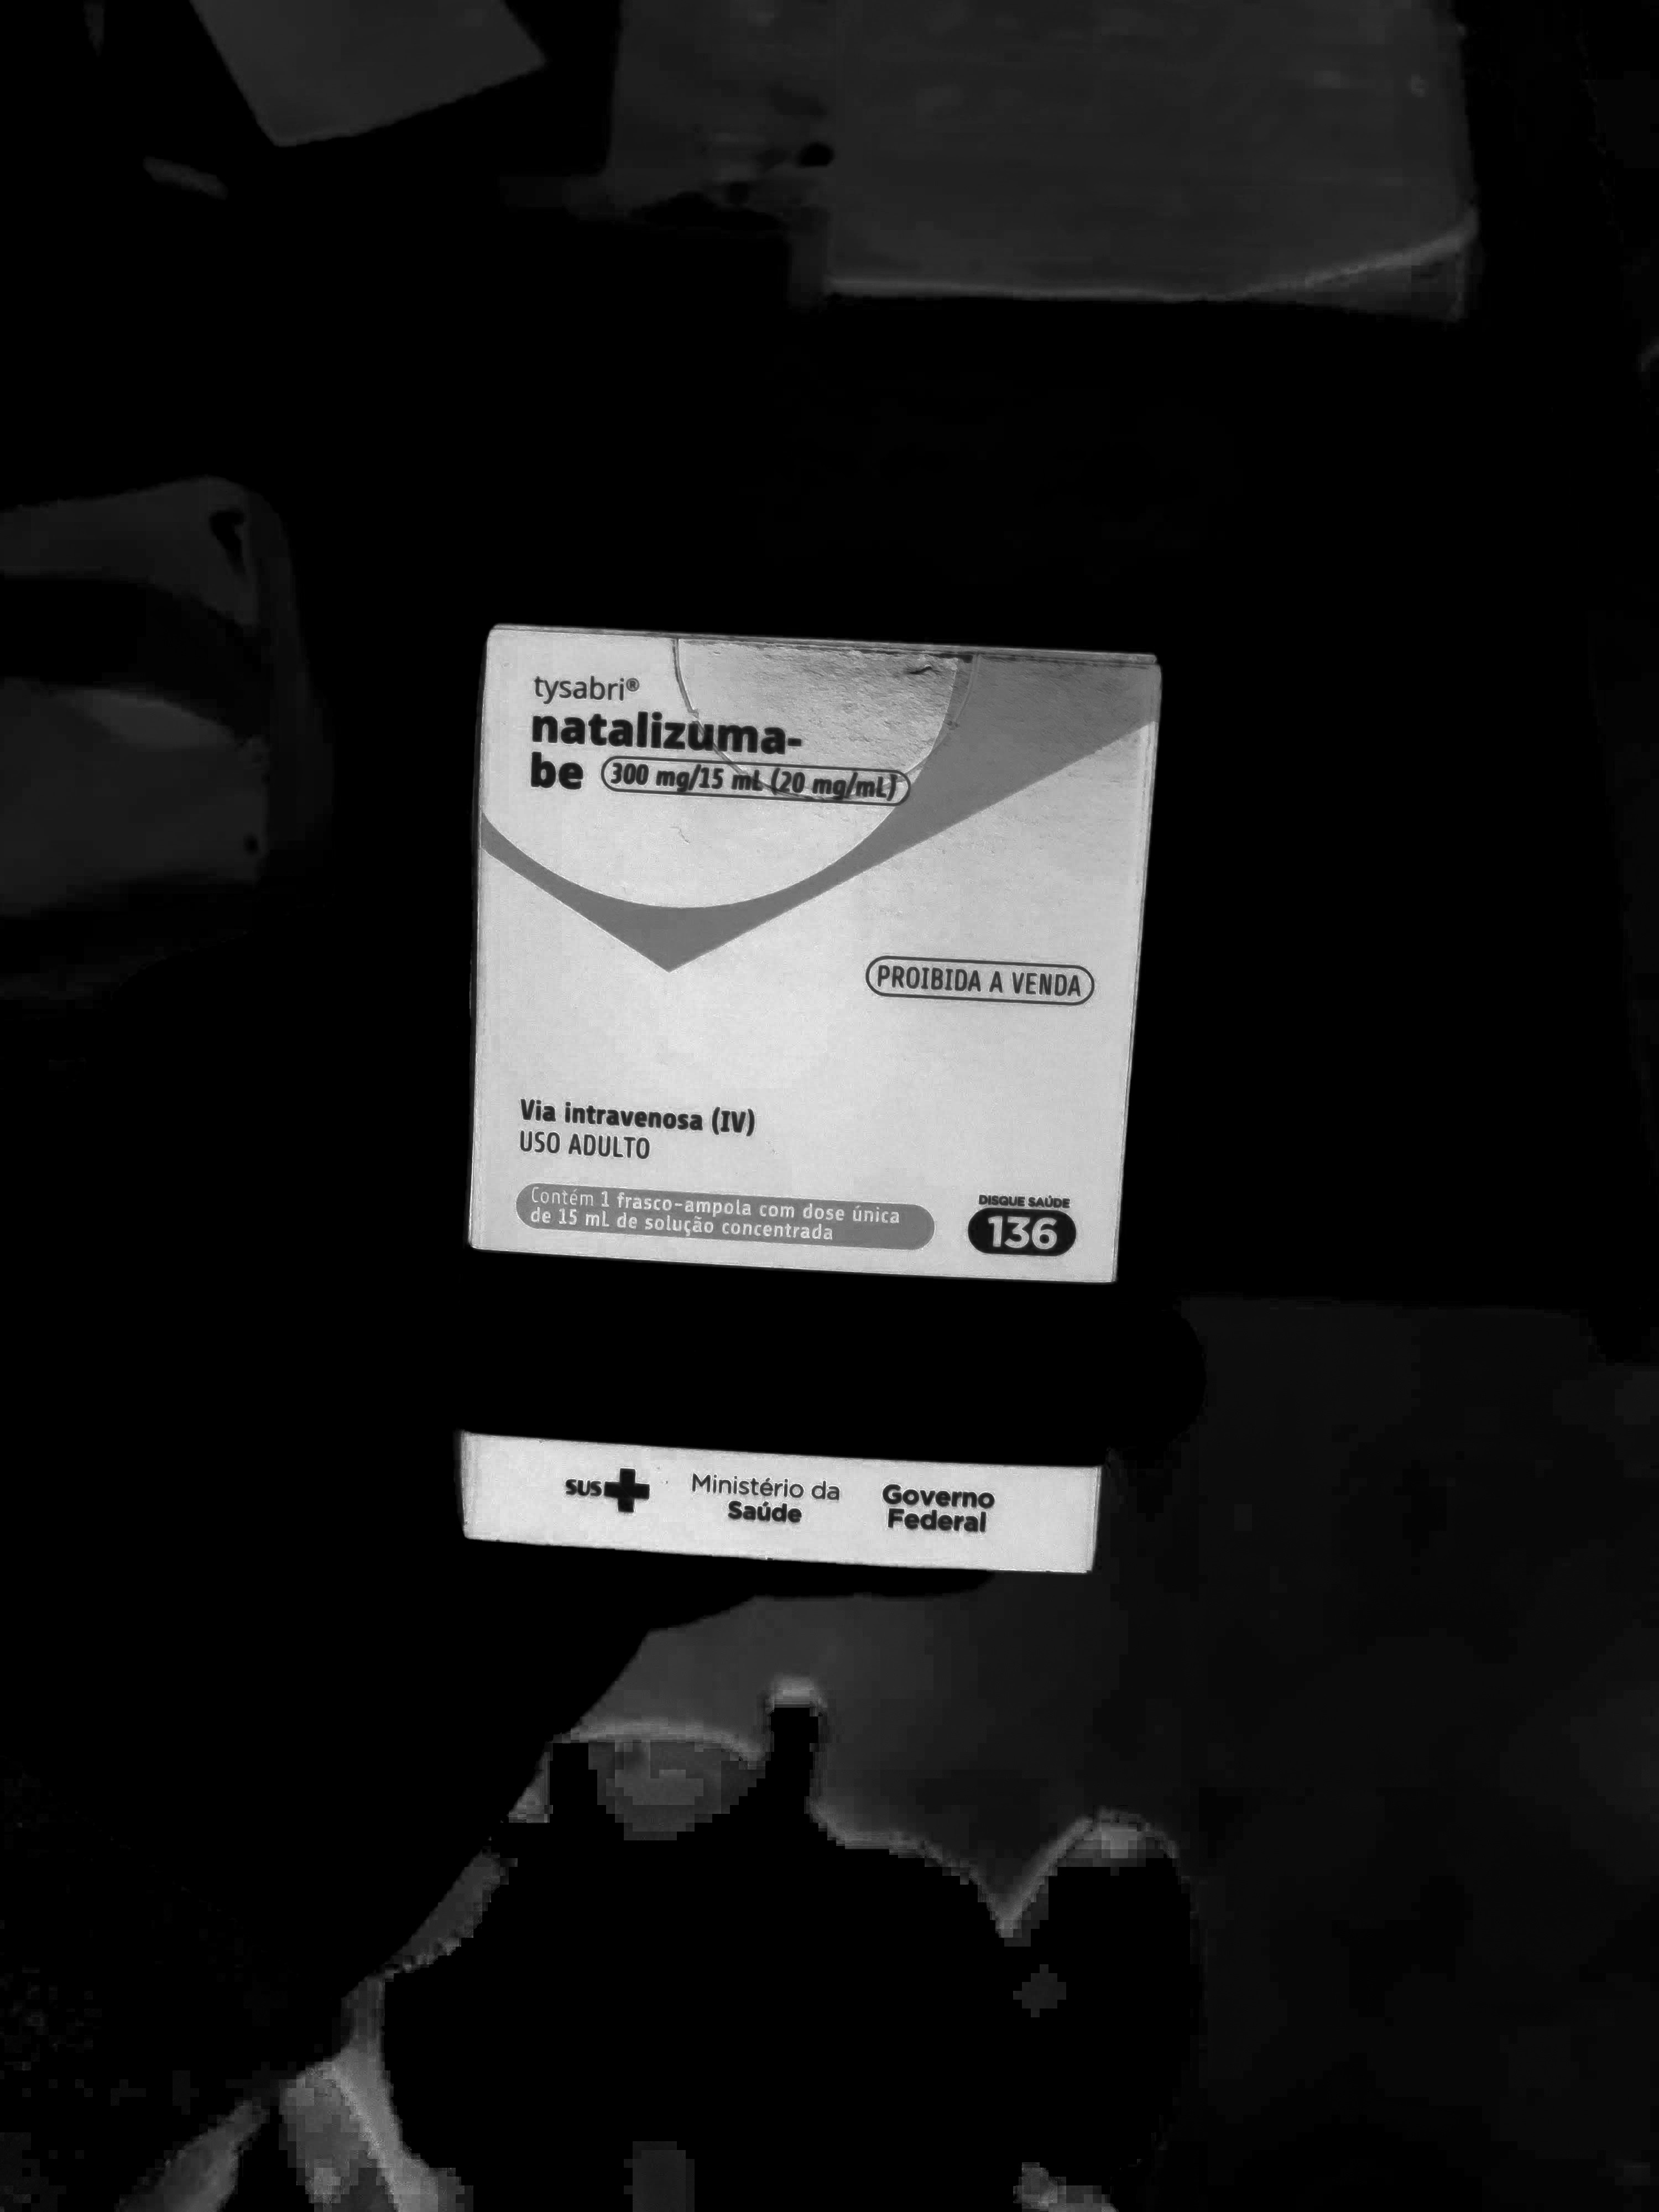
\includegraphics[width=\linewidth]{../pictures/tysabri_cmyk_c_only.jpg}
    \end{subfigure}
    \hfill
    \begin{subfigure}[t]{0.21\textwidth}
        \centering
        \caption{M.}
        \label{fig:foto:versoes:2:M}
        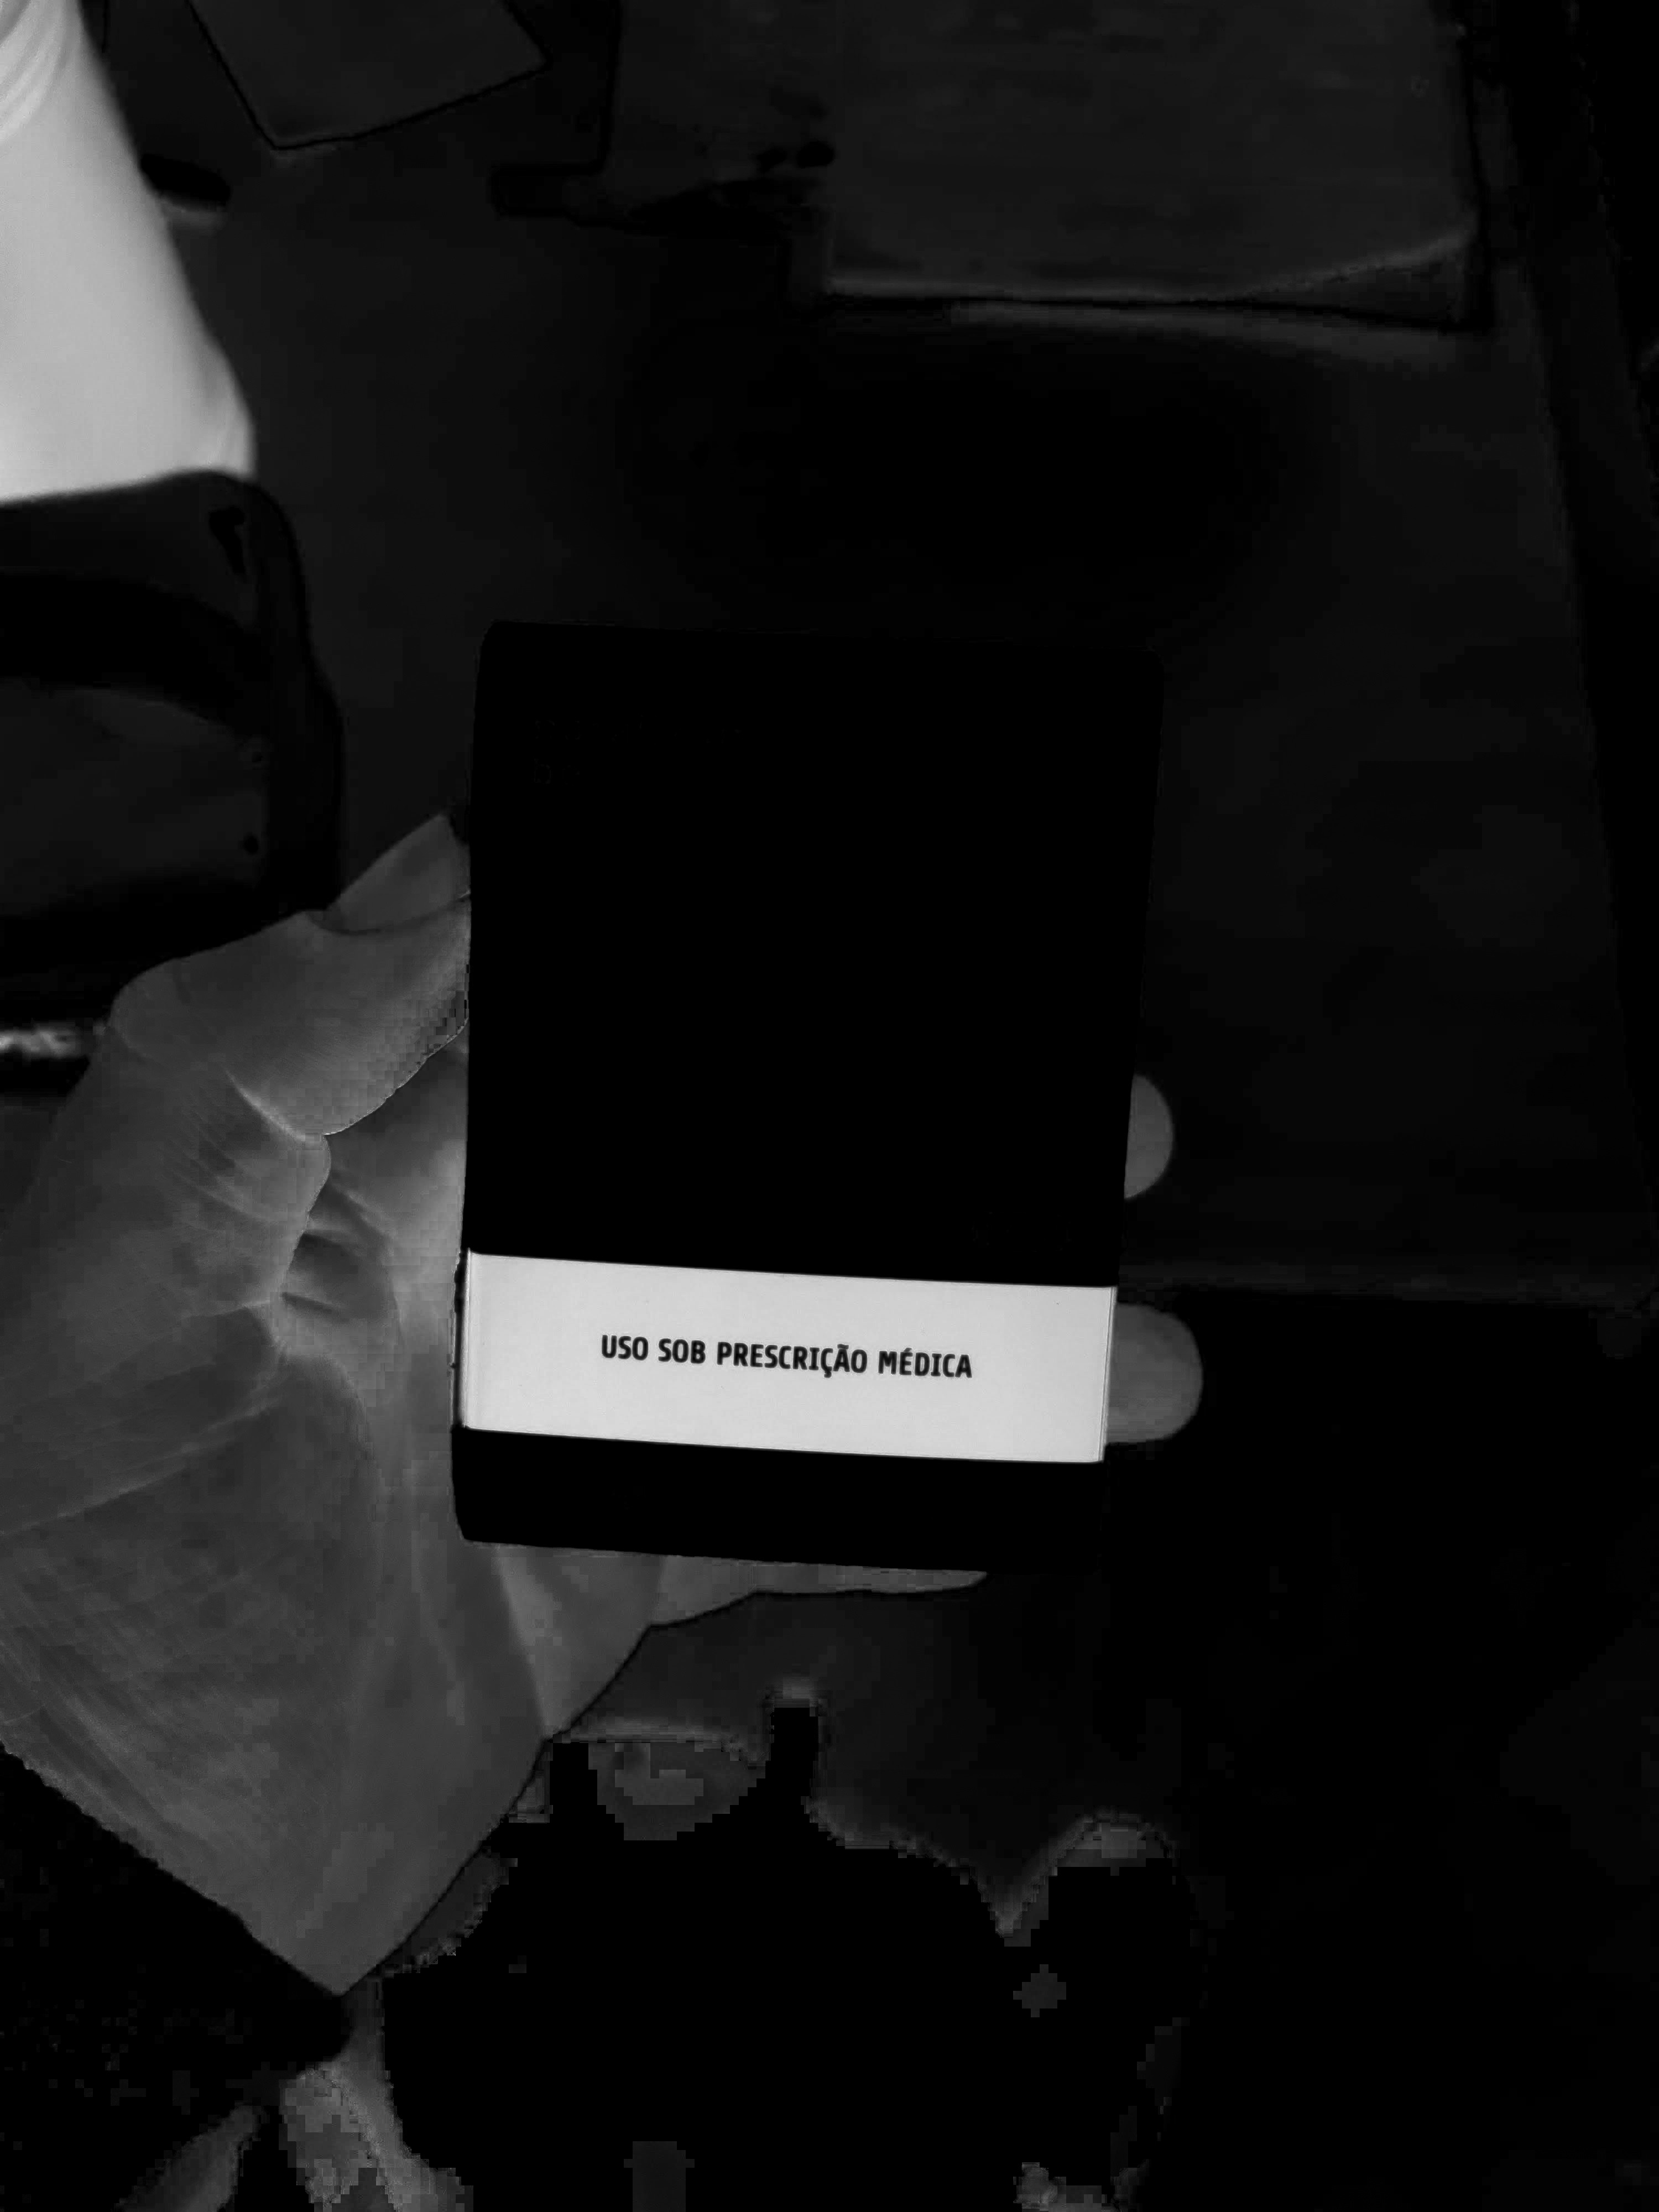
\includegraphics[width=\linewidth]{../pictures/tysabri_cmyk_m_only.jpg}
    \end{subfigure}
    \hfill
    \begin{subfigure}[t]{0.21\textwidth}
        \centering
        \caption{Y.}
        \label{fig:foto:versoes:2:Y}
        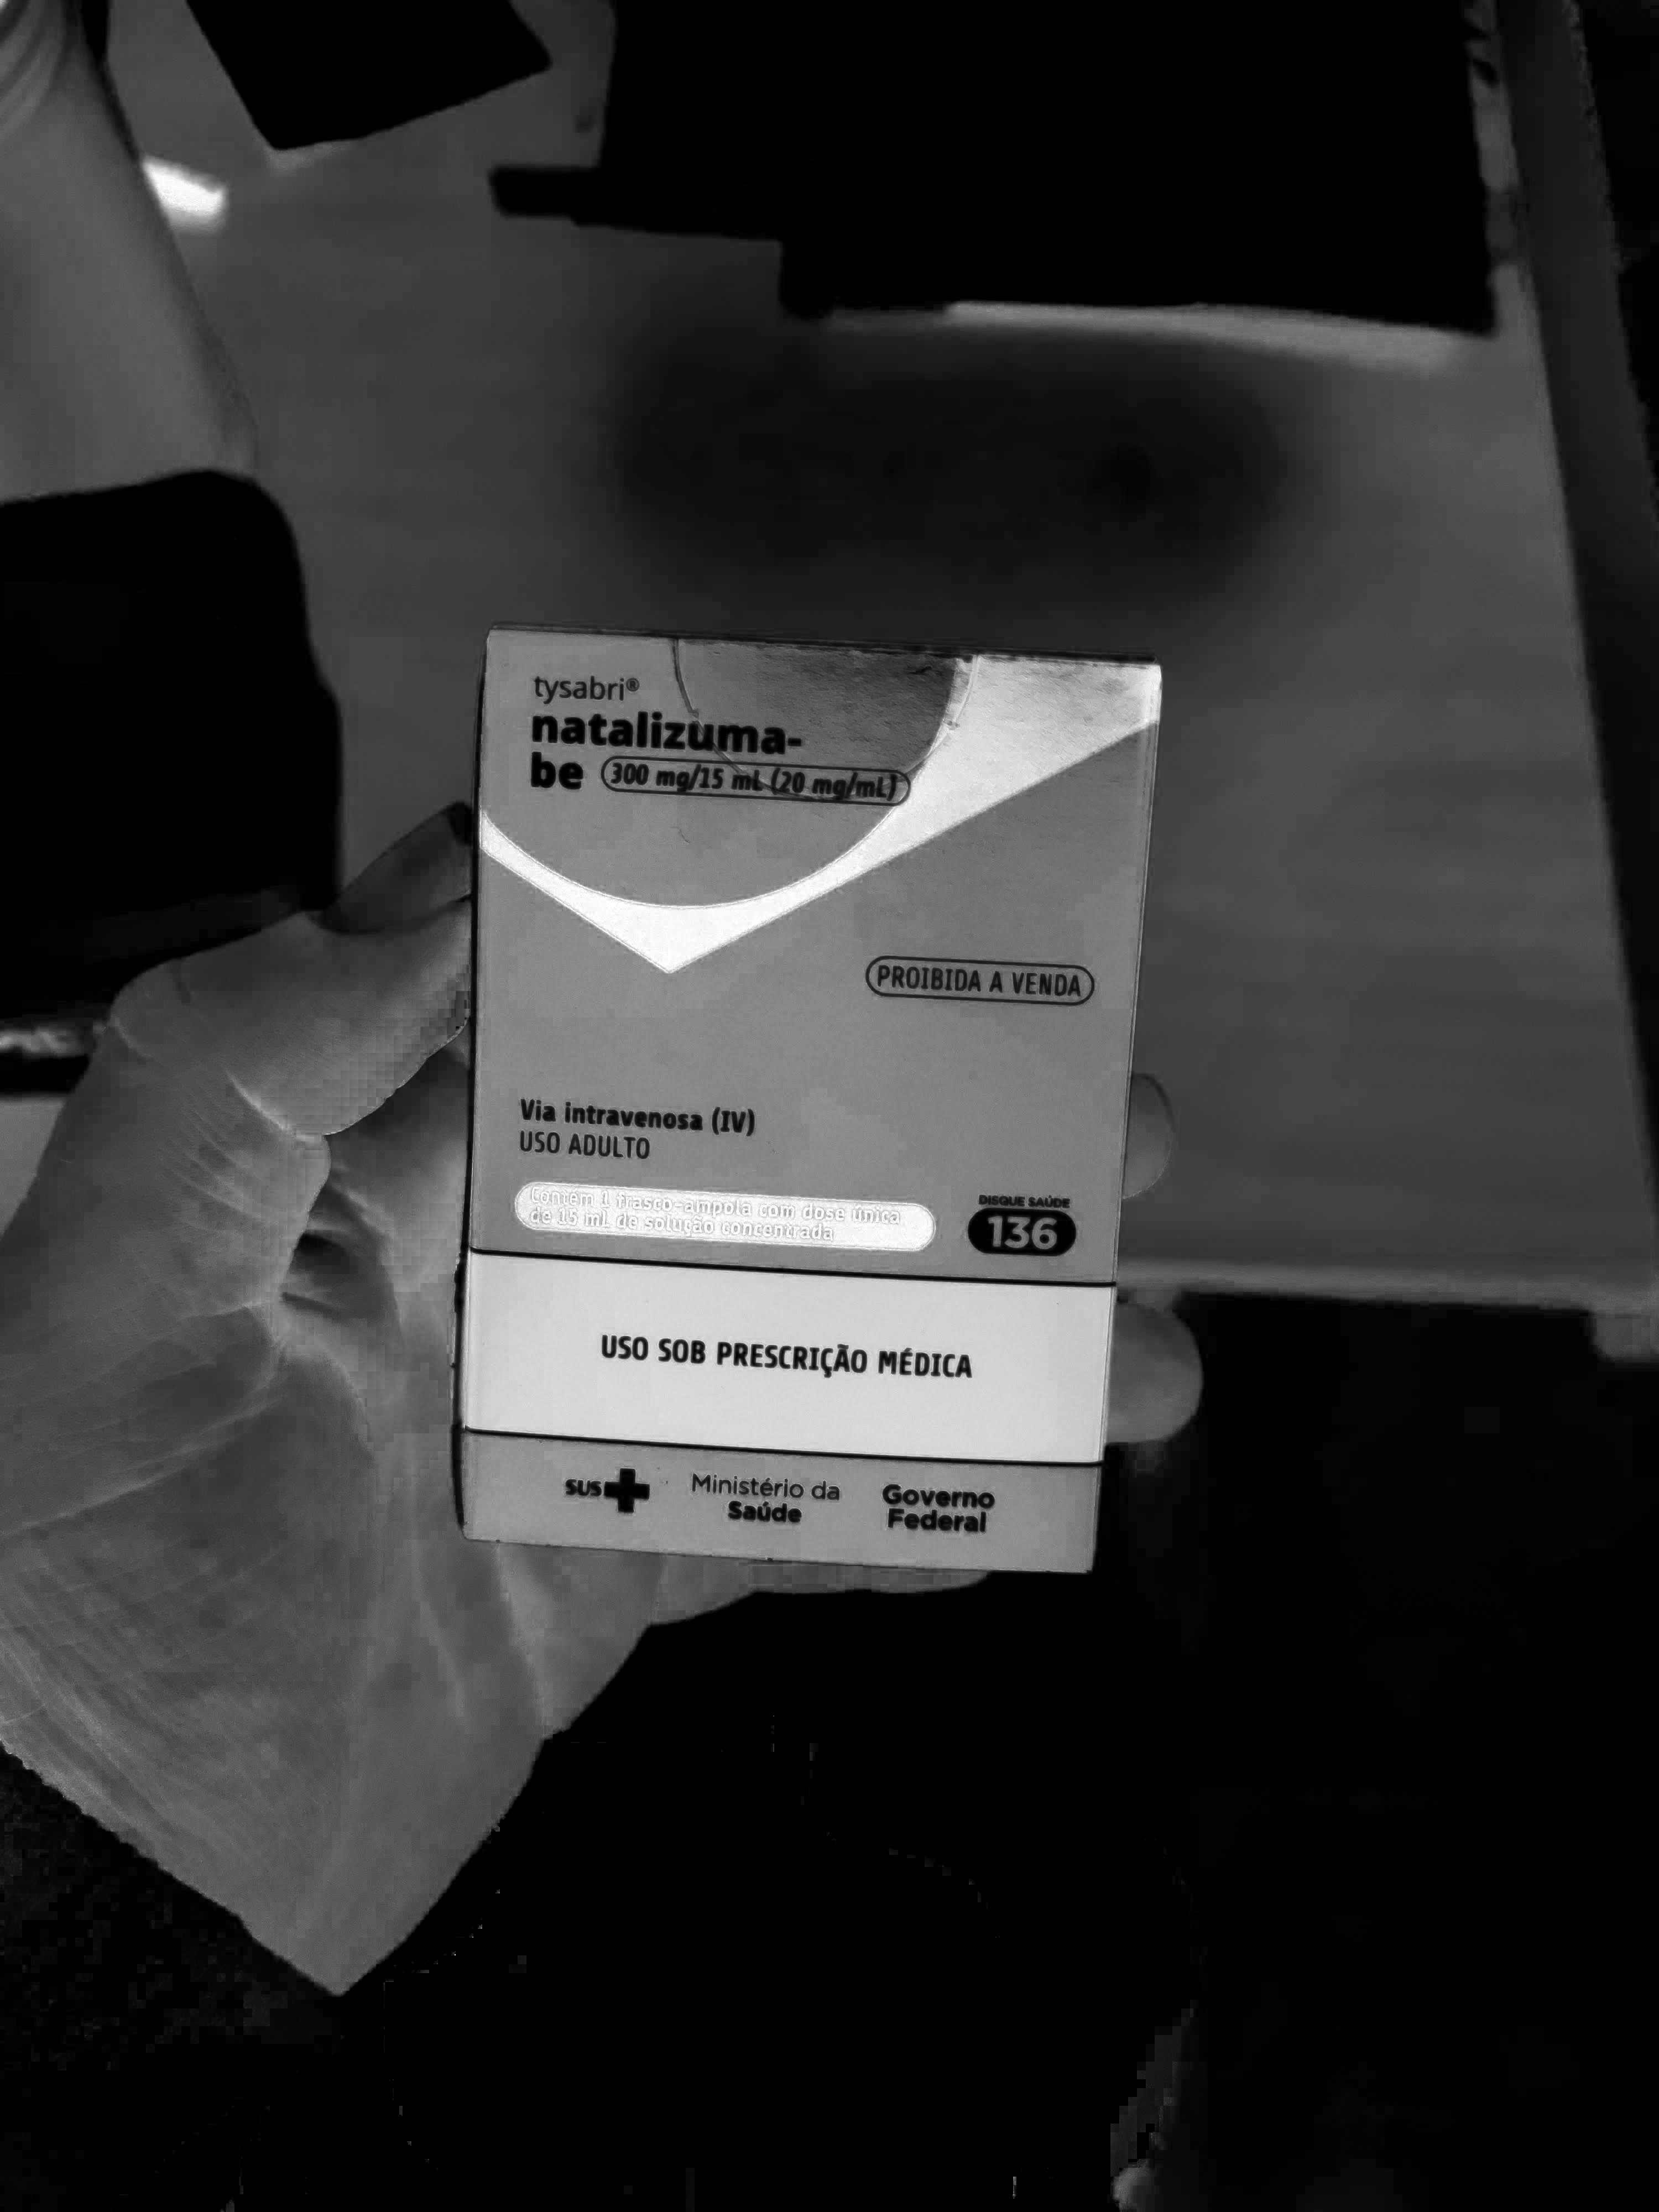
\includegraphics[width=\linewidth]{../pictures/tysabri_cmyk_y_only.jpg}
    \end{subfigure}
    \hfill
    \begin{subfigure}[t]{0.21\textwidth}
        \centering
        \caption{K.}
        \label{fig:foto:versoes:2:K}
        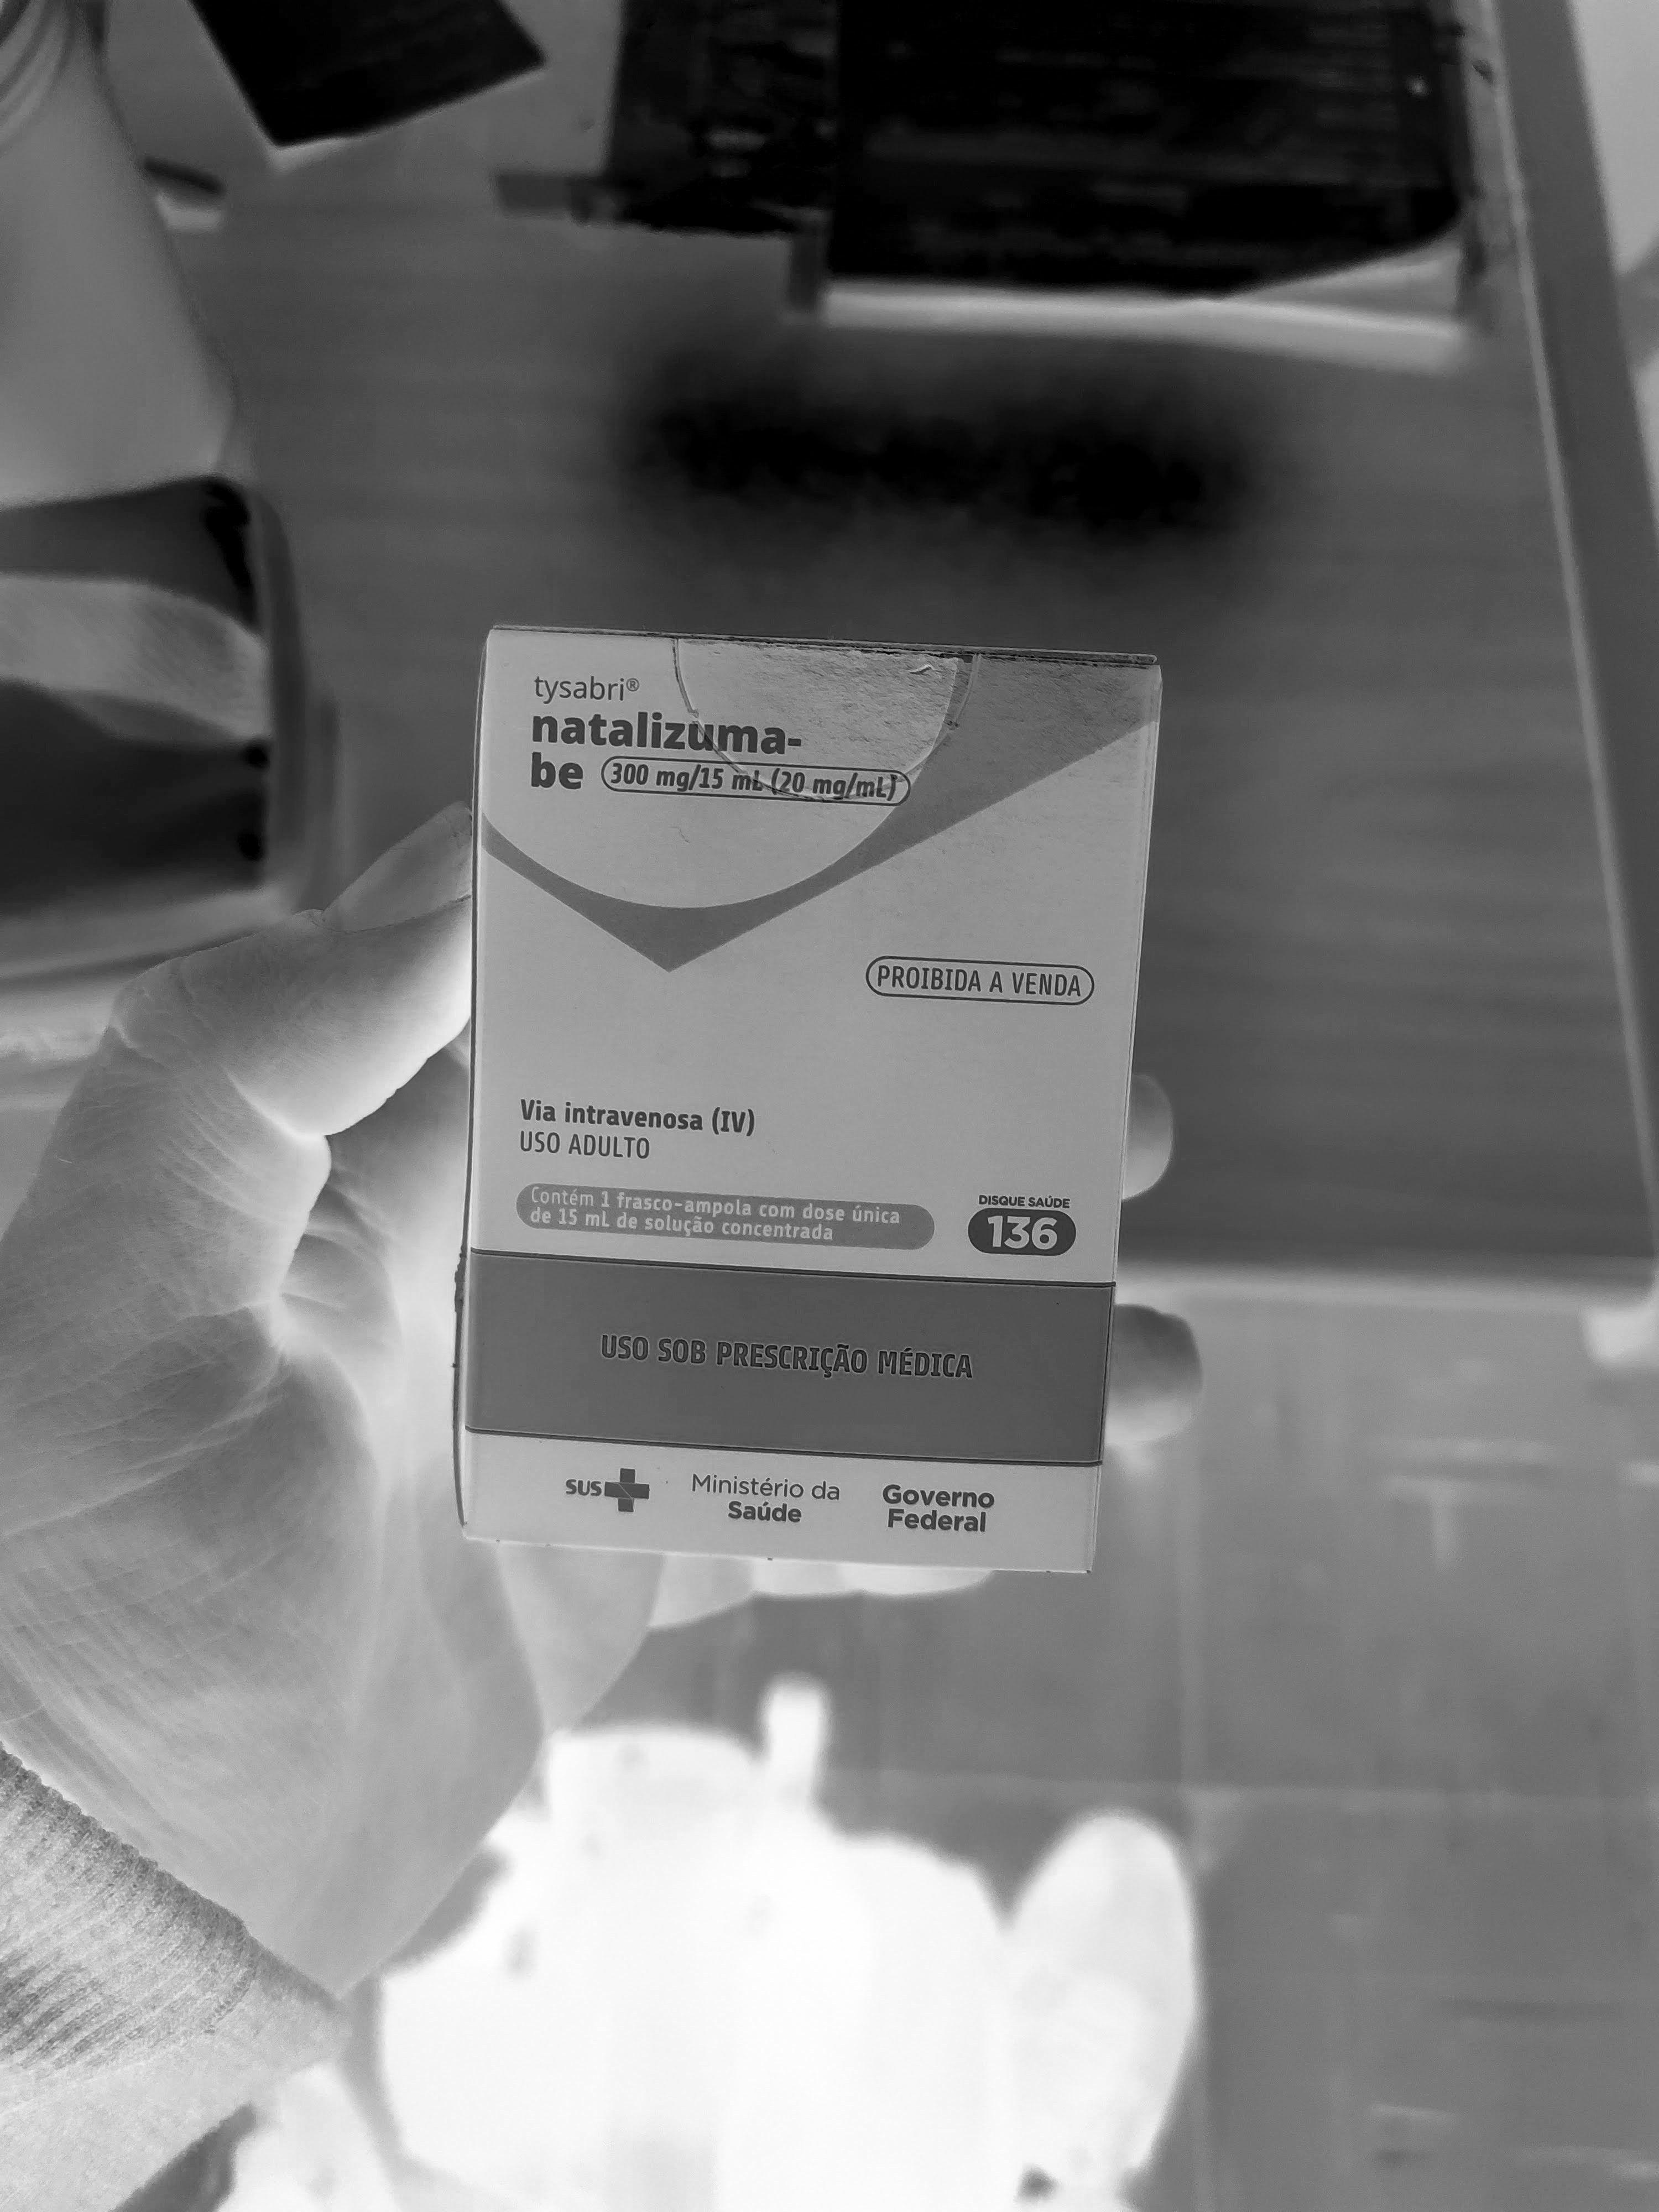
\includegraphics[width=\linewidth]{../pictures/tysabri_cmyk_k_only.jpg}
    \end{subfigure}
    \\\vspace{\floatsep}
    \begin{subfigure}[t]{0.21\textwidth}
        \centering
        \caption{C.}
        \label{fig:foto:versoes:2:C:boxes}
        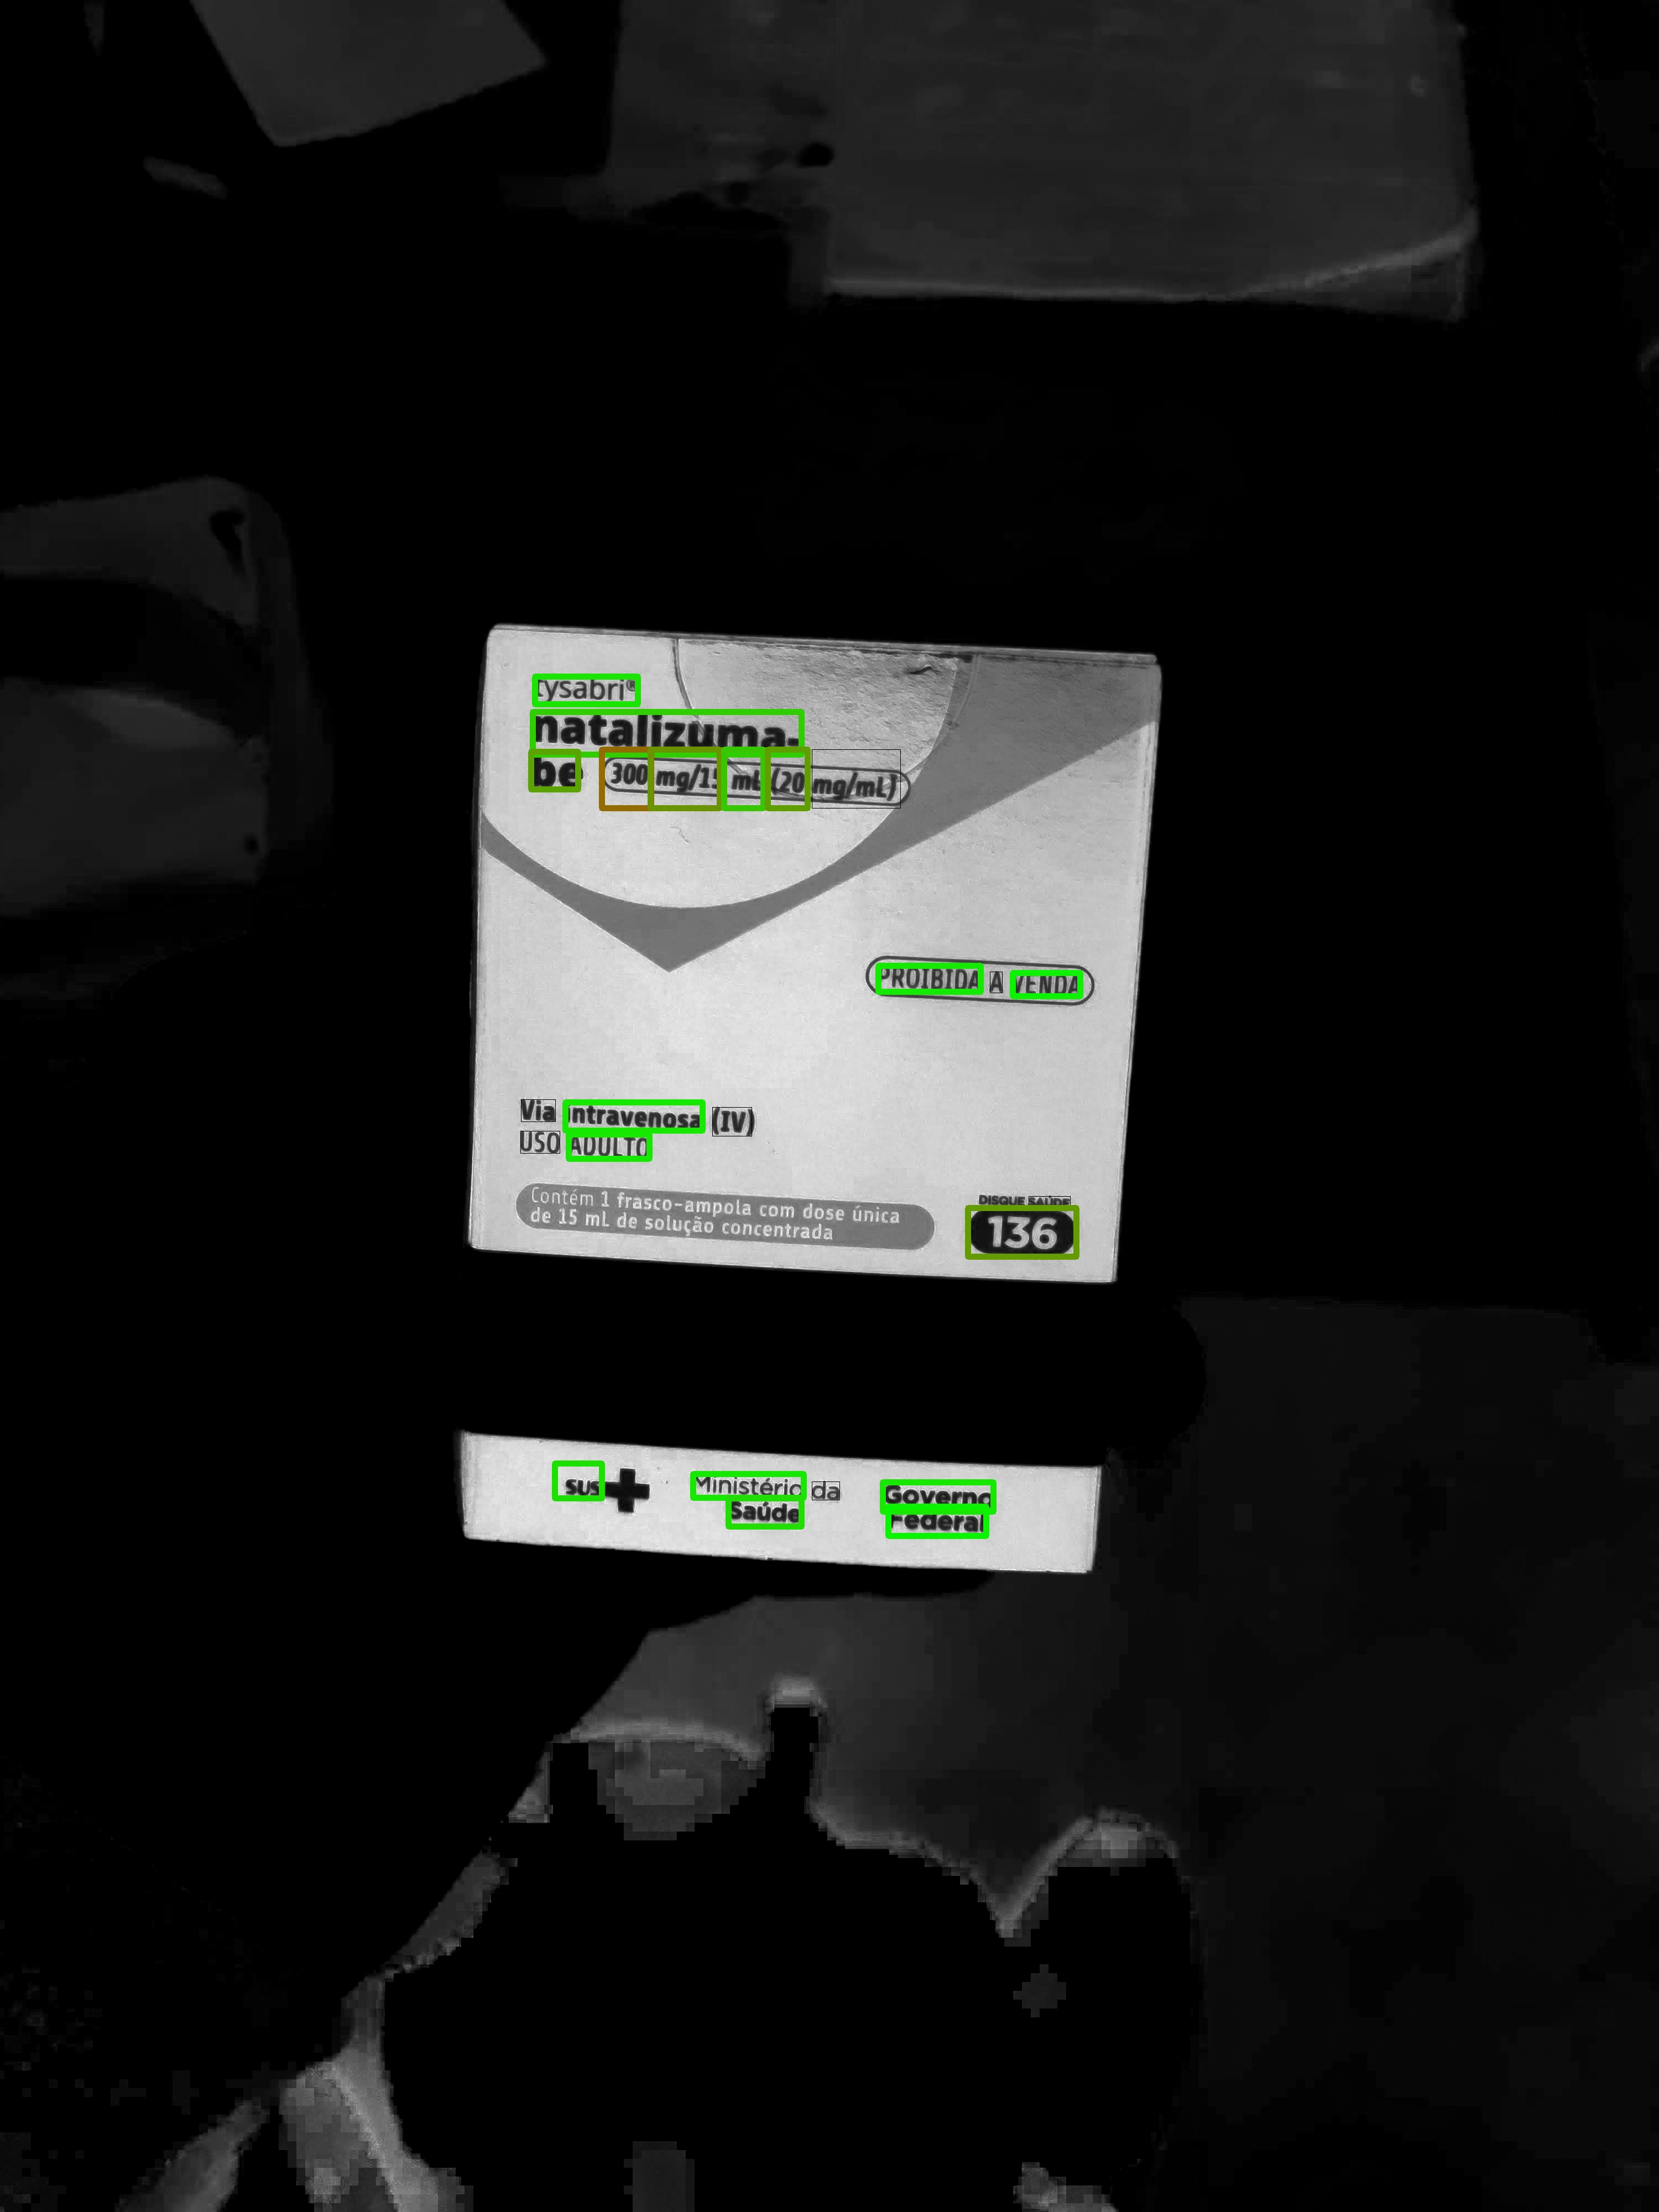
\includegraphics[width=\linewidth]{../pictures/tysabri_cmyk_c_only_boxes.jpg}
    \end{subfigure}
    \hfill
    \begin{subfigure}[t]{0.21\textwidth}
        \centering
        \caption{M.}
        \label{fig:foto:versoes:2:M:boxes}
        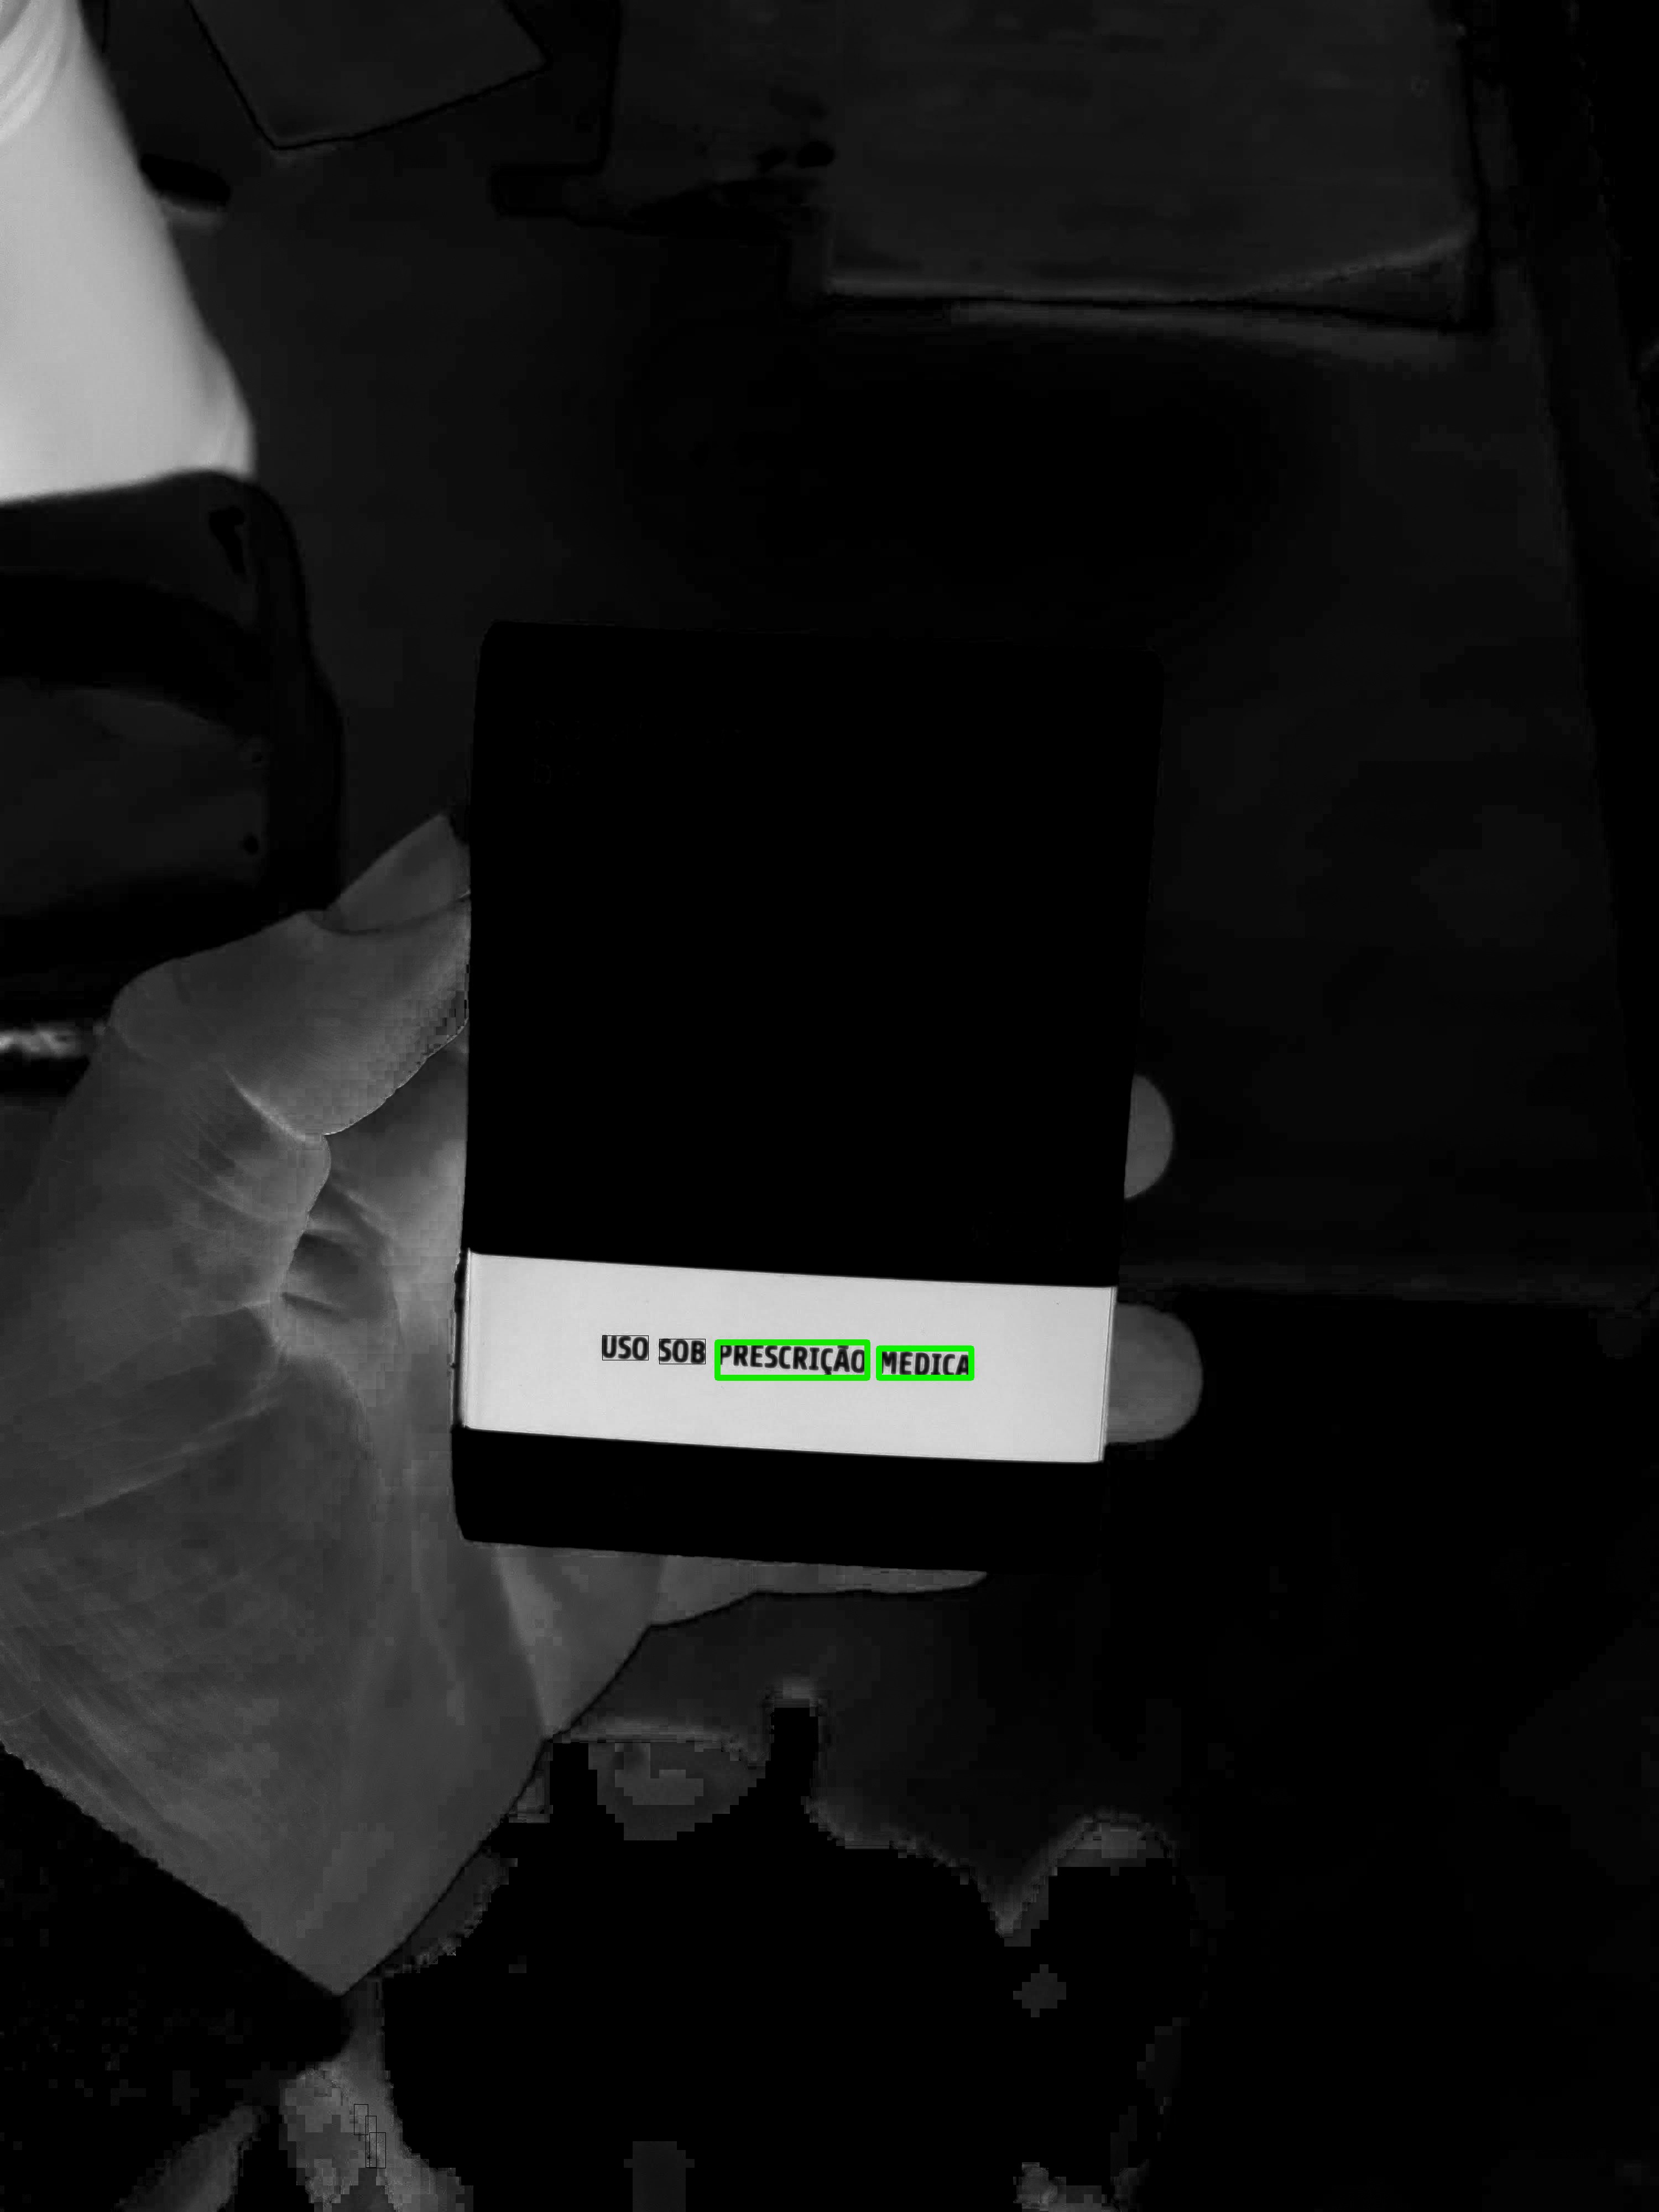
\includegraphics[width=\linewidth]{../pictures/tysabri_cmyk_m_only_boxes.jpg}
    \end{subfigure}
    \hfill
    \begin{subfigure}[t]{0.21\textwidth}
        \centering
        \caption{Y.}
        \label{fig:foto:versoes:2:Y:boxes}
        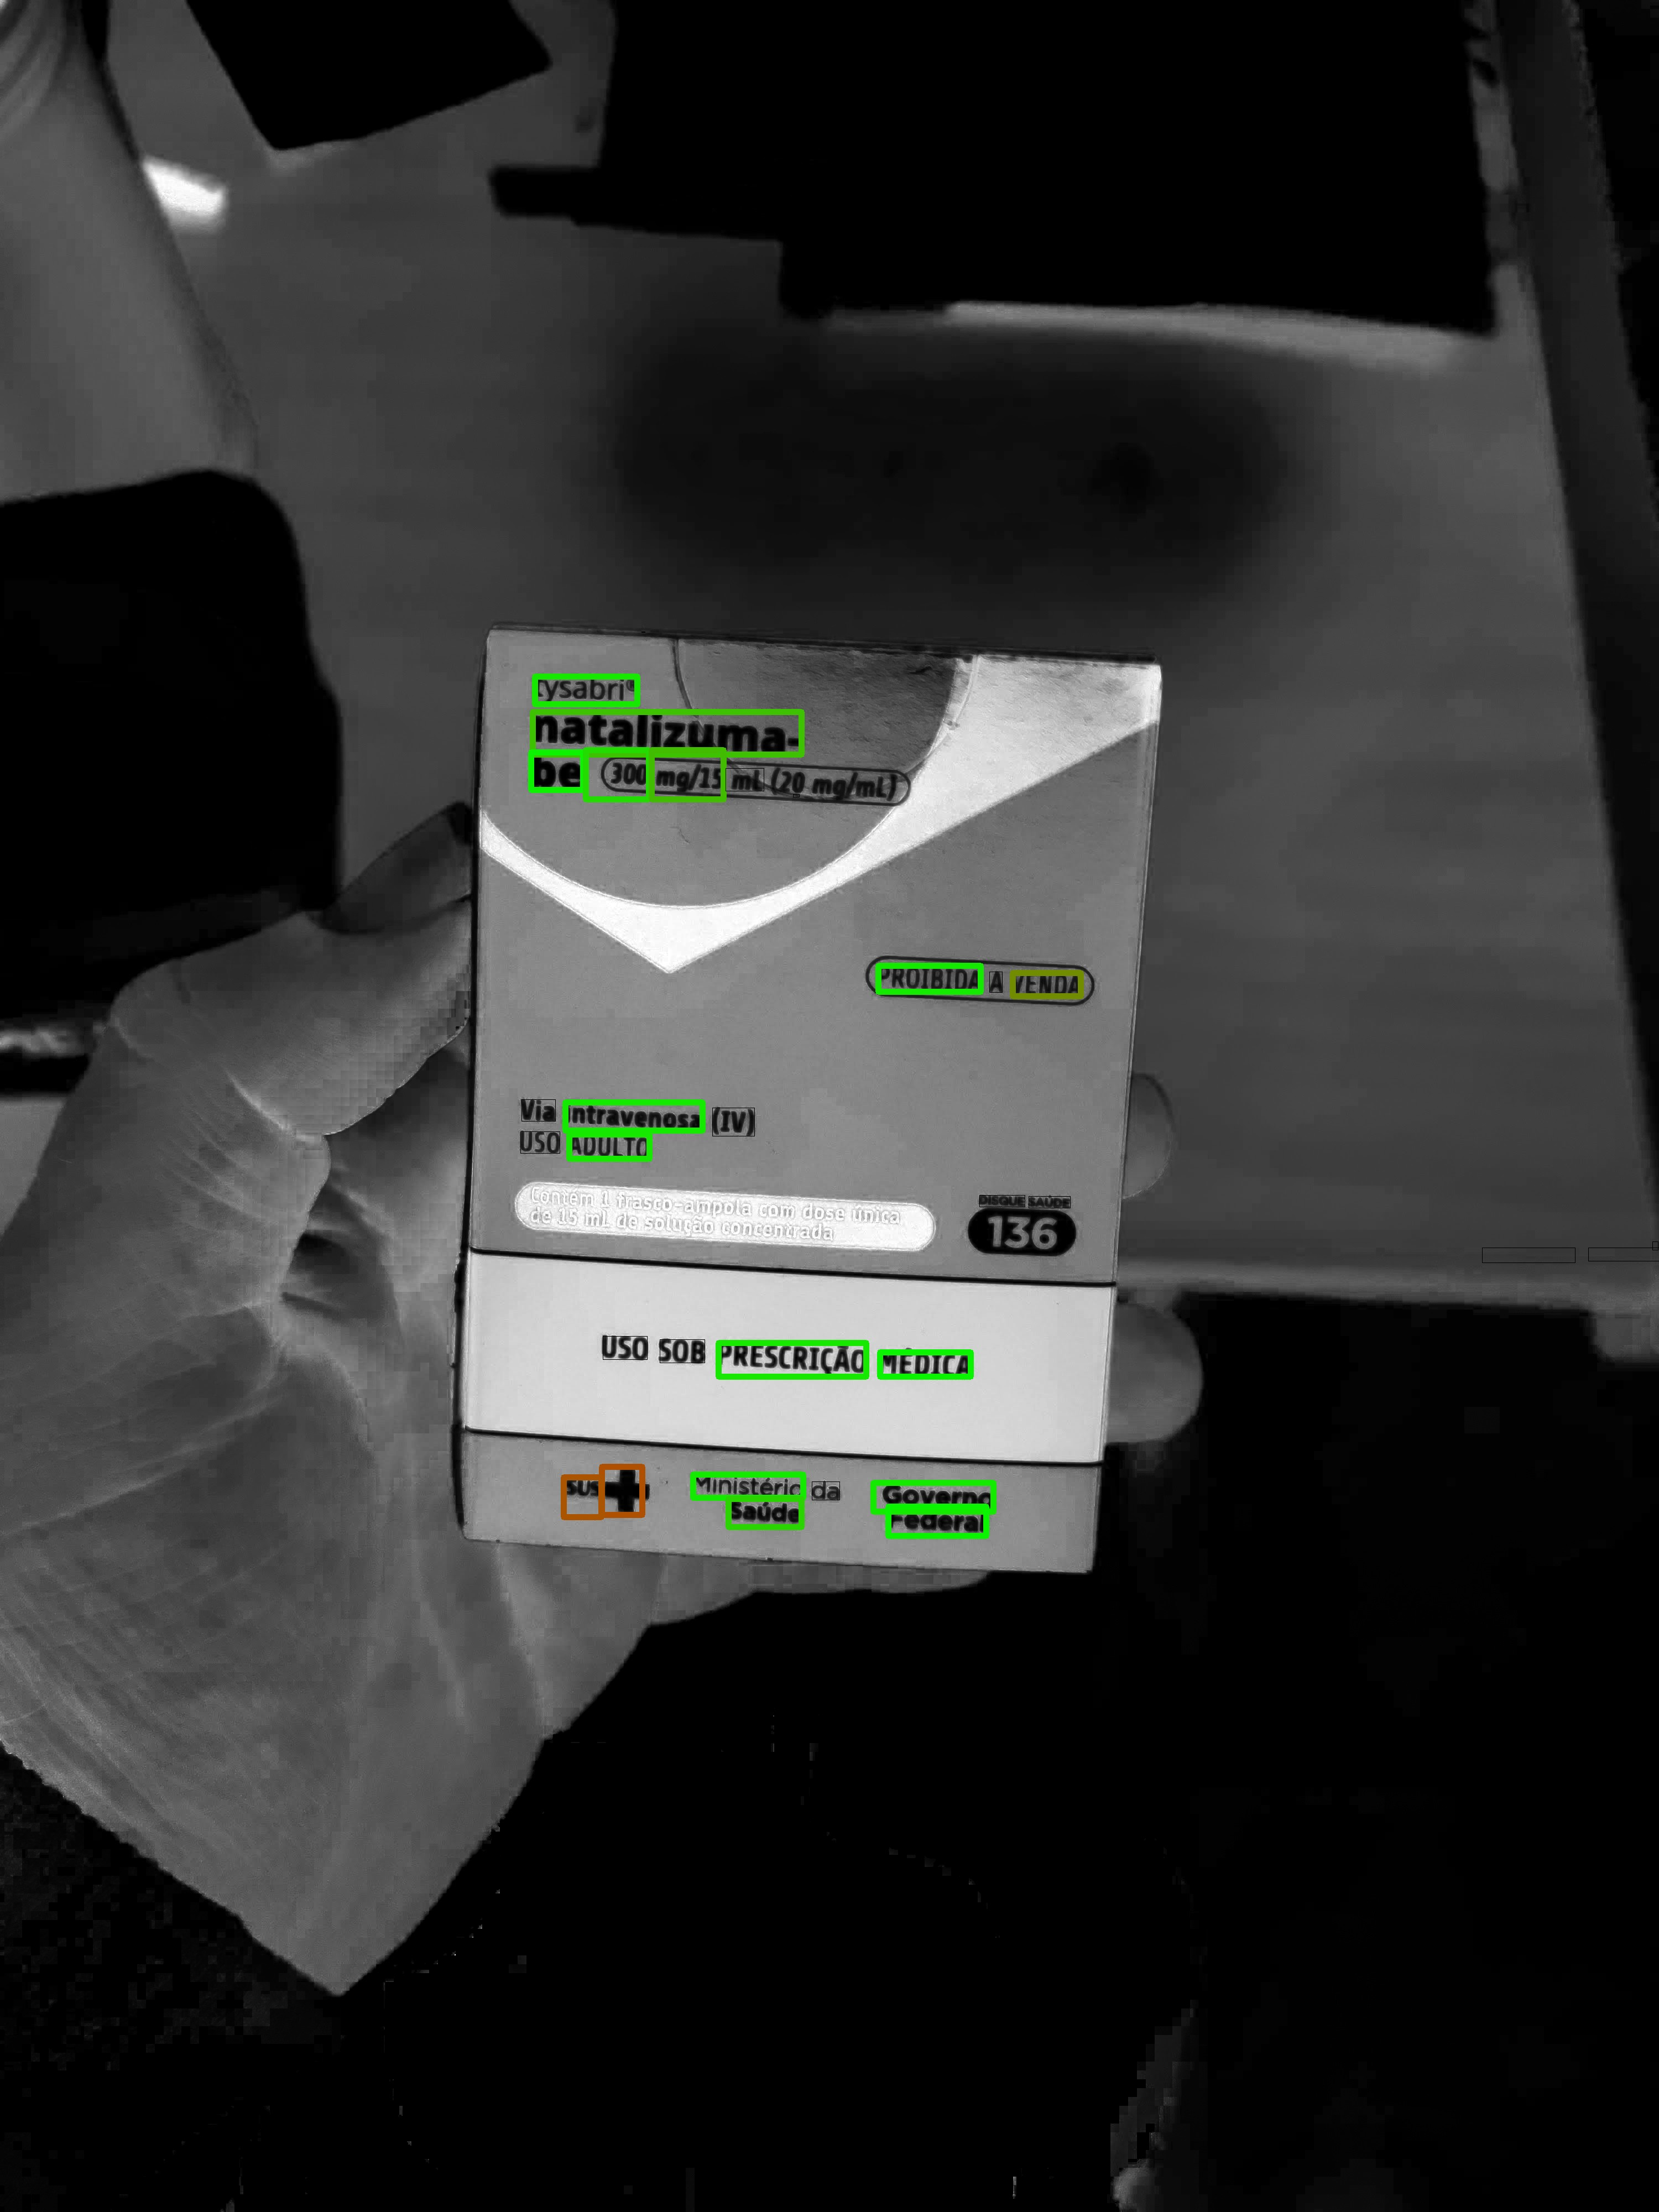
\includegraphics[width=\linewidth]{../pictures/tysabri_cmyk_y_only_boxes.jpg}
    \end{subfigure}
    \hfill
    \begin{subfigure}[t]{0.21\textwidth}
        \centering
        \caption{K.}
        \label{fig:foto:versoes:2:K:boxes}
        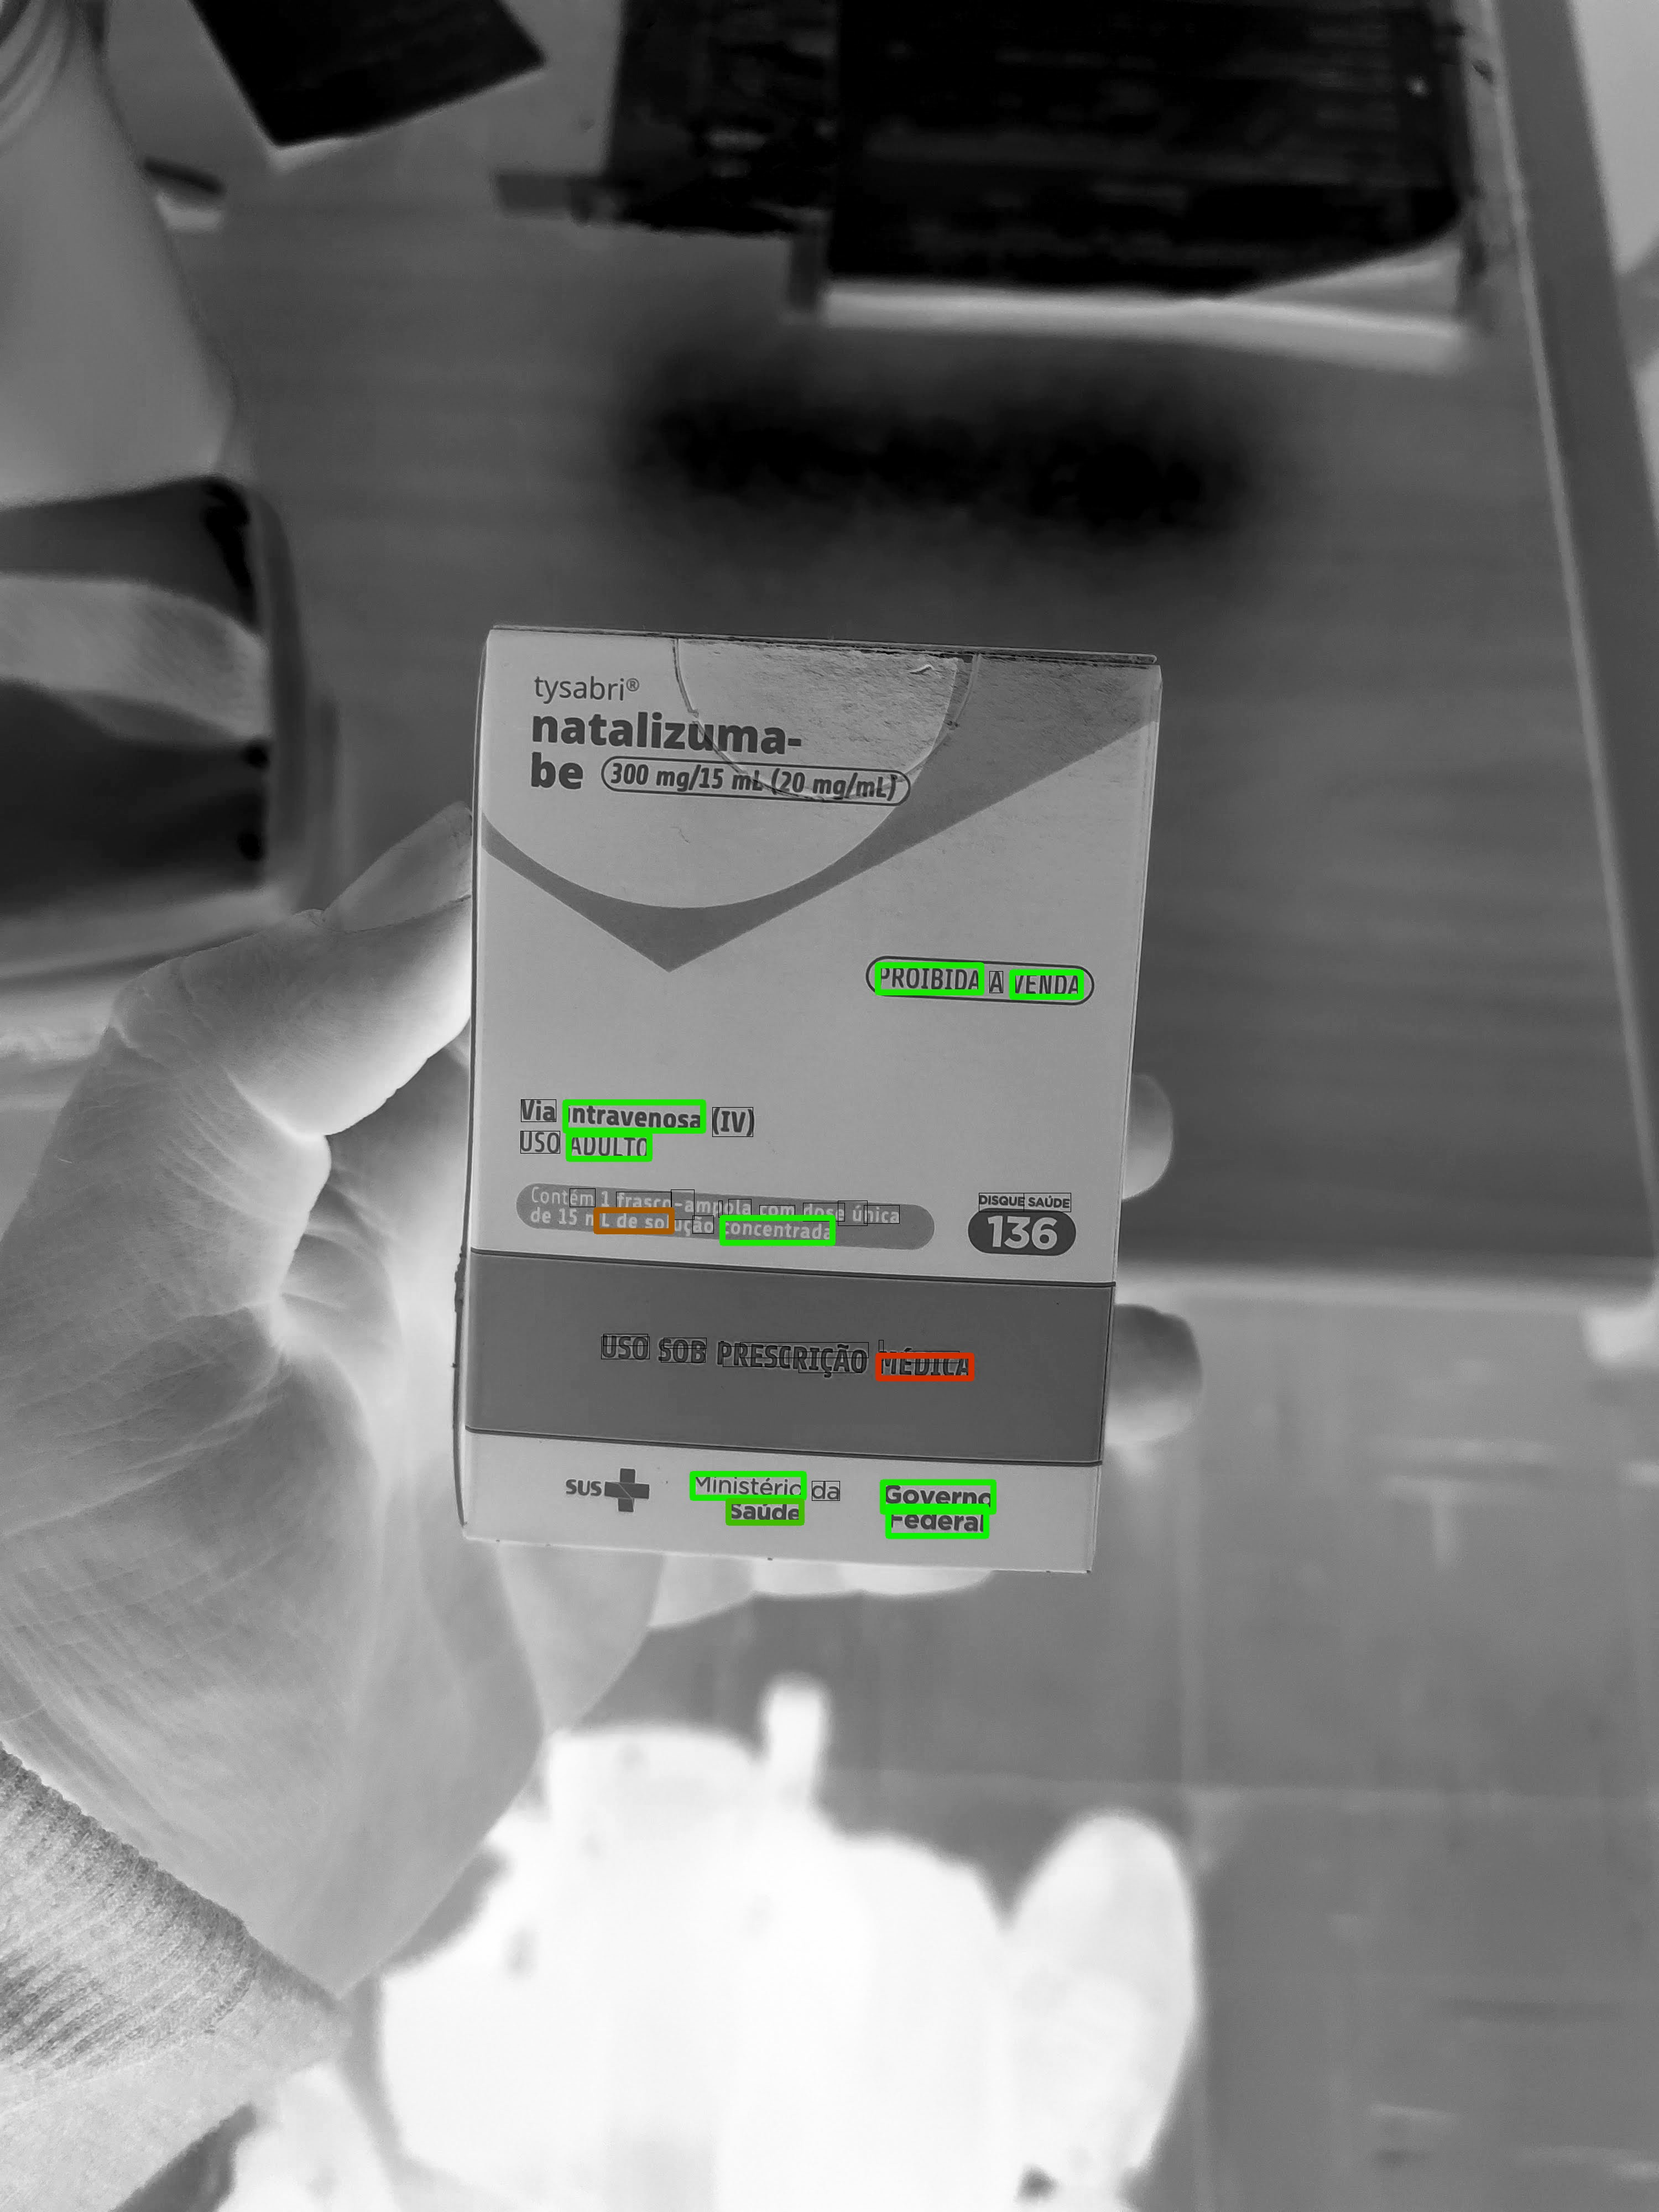
\includegraphics[width=\linewidth]{../pictures/tysabri_cmyk_k_only_boxes.jpg}
    \end{subfigure}
    \\\vspace{\floatsep}
    \begin{subfigure}[t]{0.21\textwidth}
        \centering
        \caption{C thresh.}
        \label{fig:foto:versoes:2:C_thresh}
        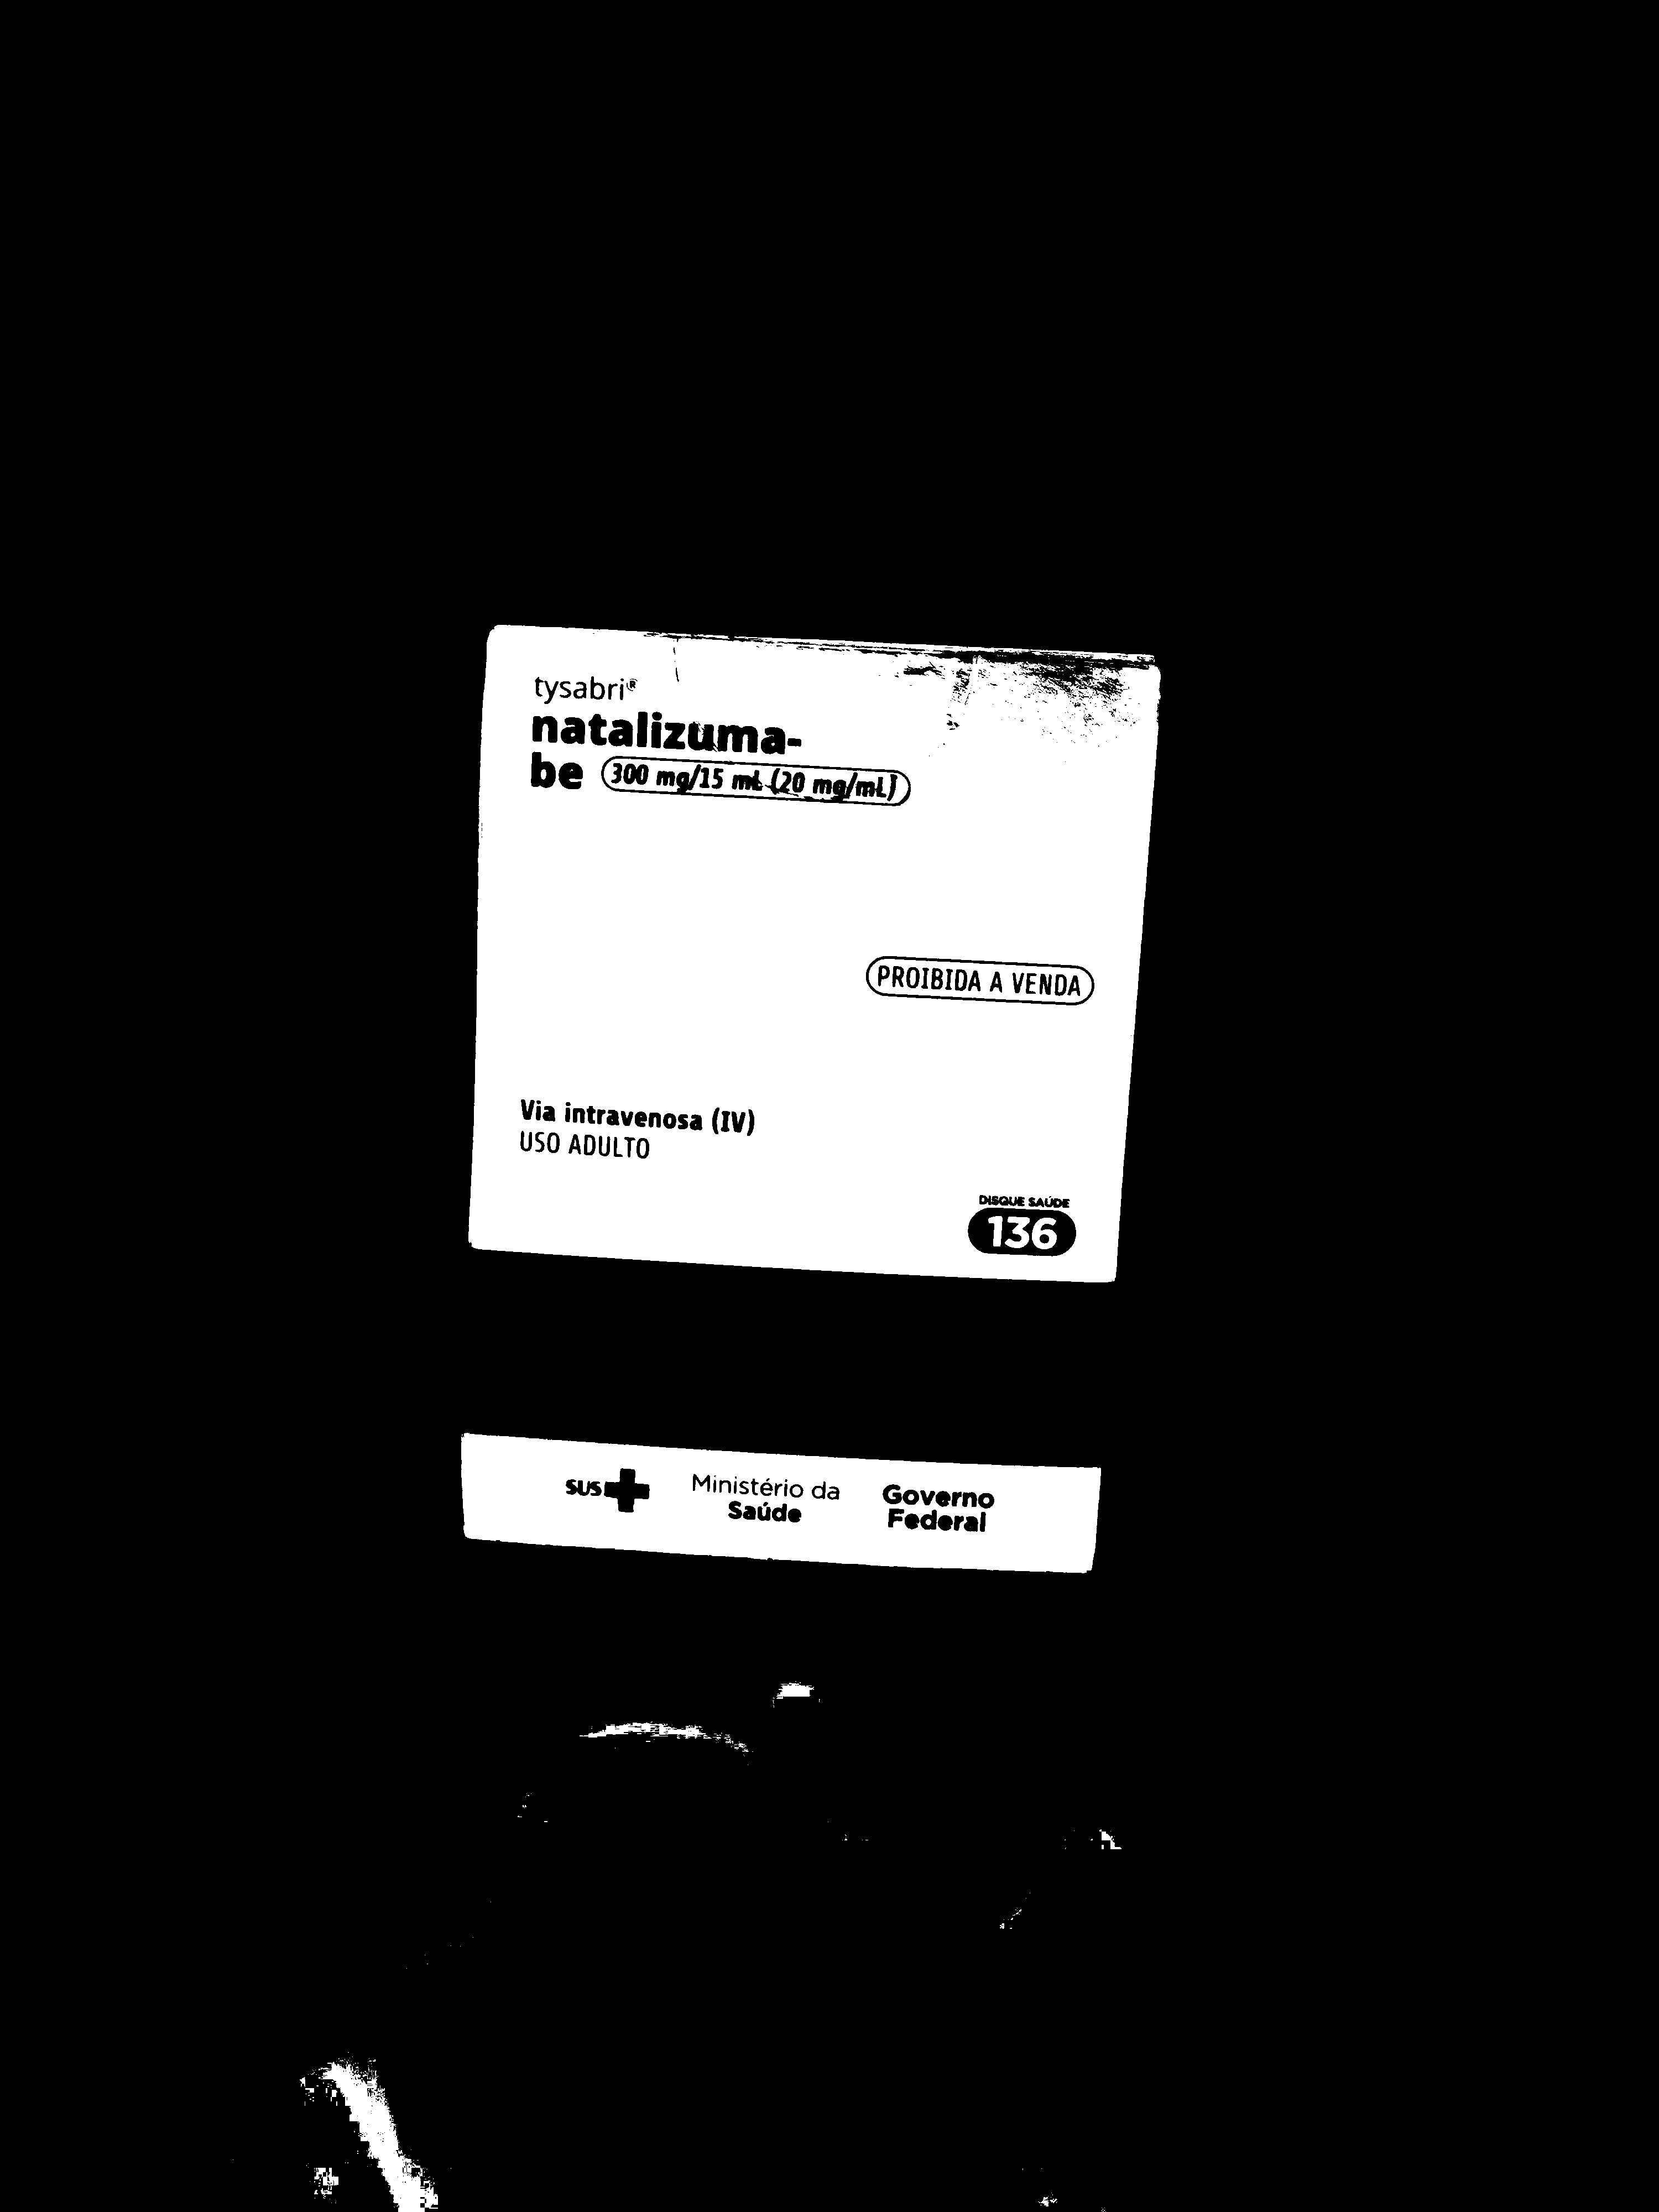
\includegraphics[width=\linewidth]{../pictures/tysabri_cmyk_c_only_thresh.jpg}
    \end{subfigure}
    \hfill
    \begin{subfigure}[t]{0.21\textwidth}
        \centering
        \caption{M thresh.}
        \label{fig:foto:versoes:2:M_thresh}
        
\includegraphics[width=\linewidth]{../pictures/tysabri_cmyk_m_only_thresh.jpg}
    \end{subfigure}
    \hfill
    \begin{subfigure}[t]{0.21\textwidth}
        \centering
        \caption{Y thresh.}
        \label{fig:foto:versoes:2:Y_thresh}
        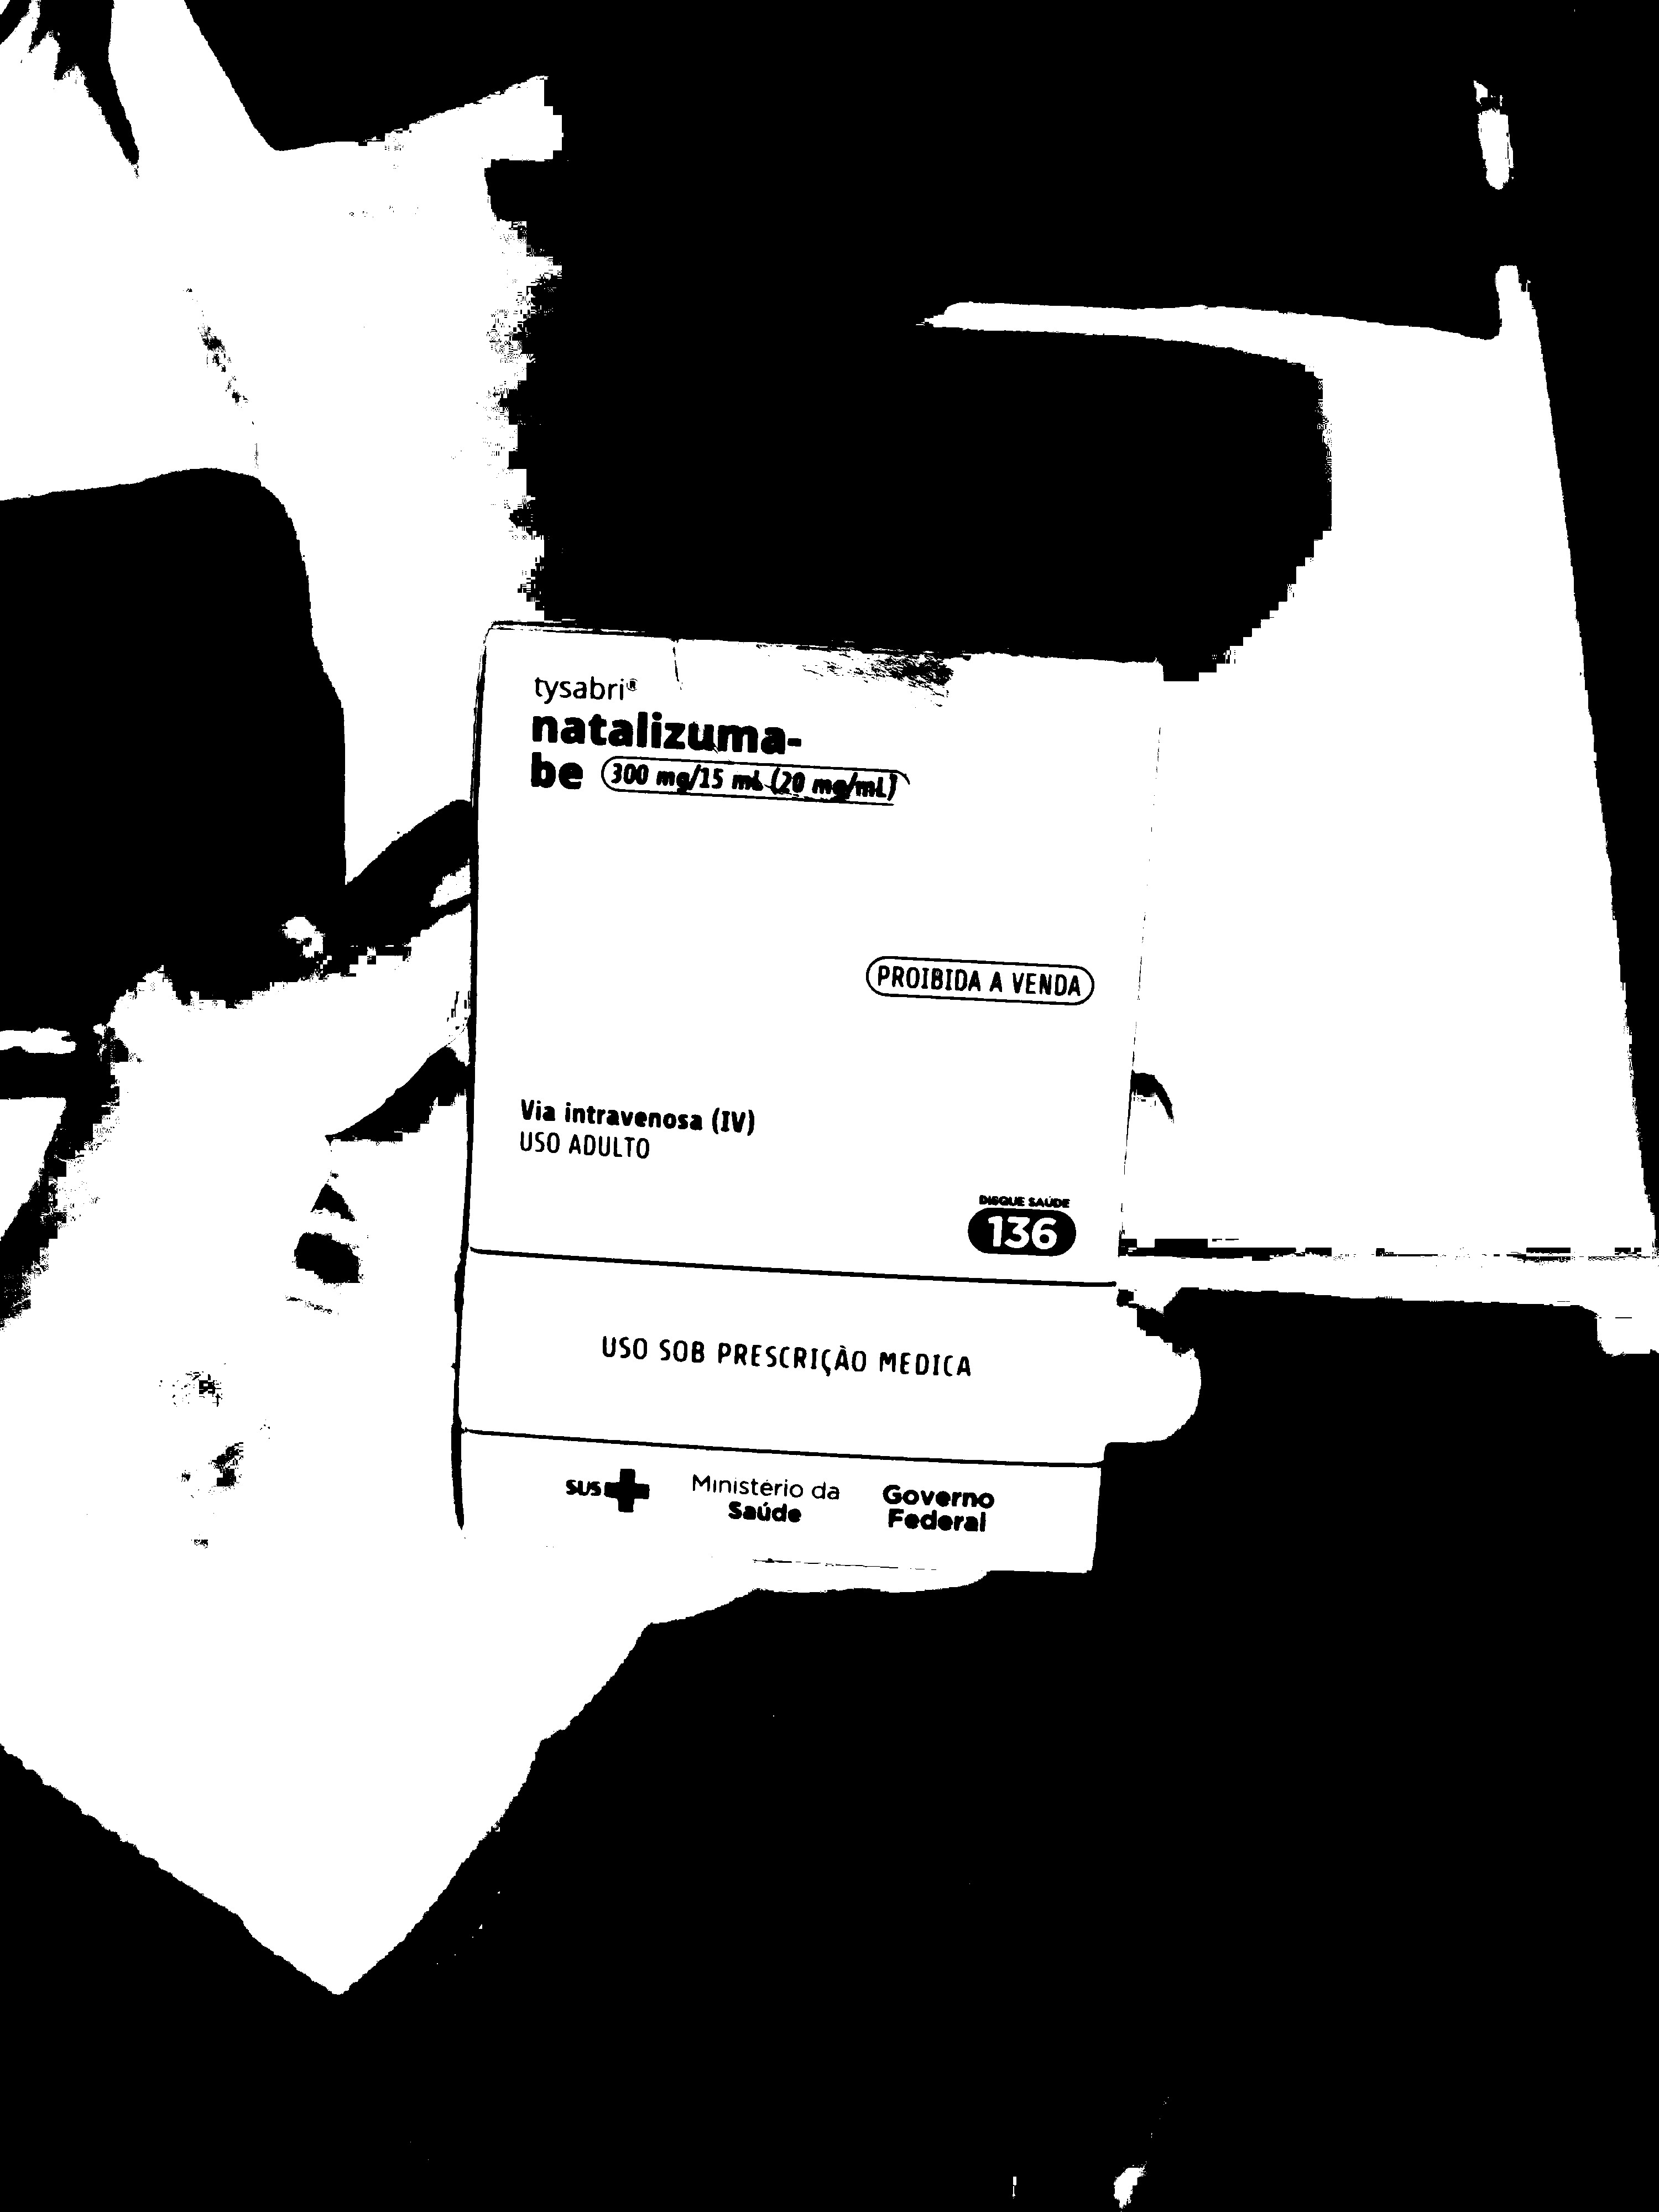
\includegraphics[width=\linewidth]{../pictures/tysabri_cmyk_y_only_thresh.jpg}
    \end{subfigure}
    \hfill
    \begin{subfigure}[t]{0.21\textwidth}
        \centering
        \caption{K thresh.}
        \label{fig:foto:versoes:2:K_thresh}
        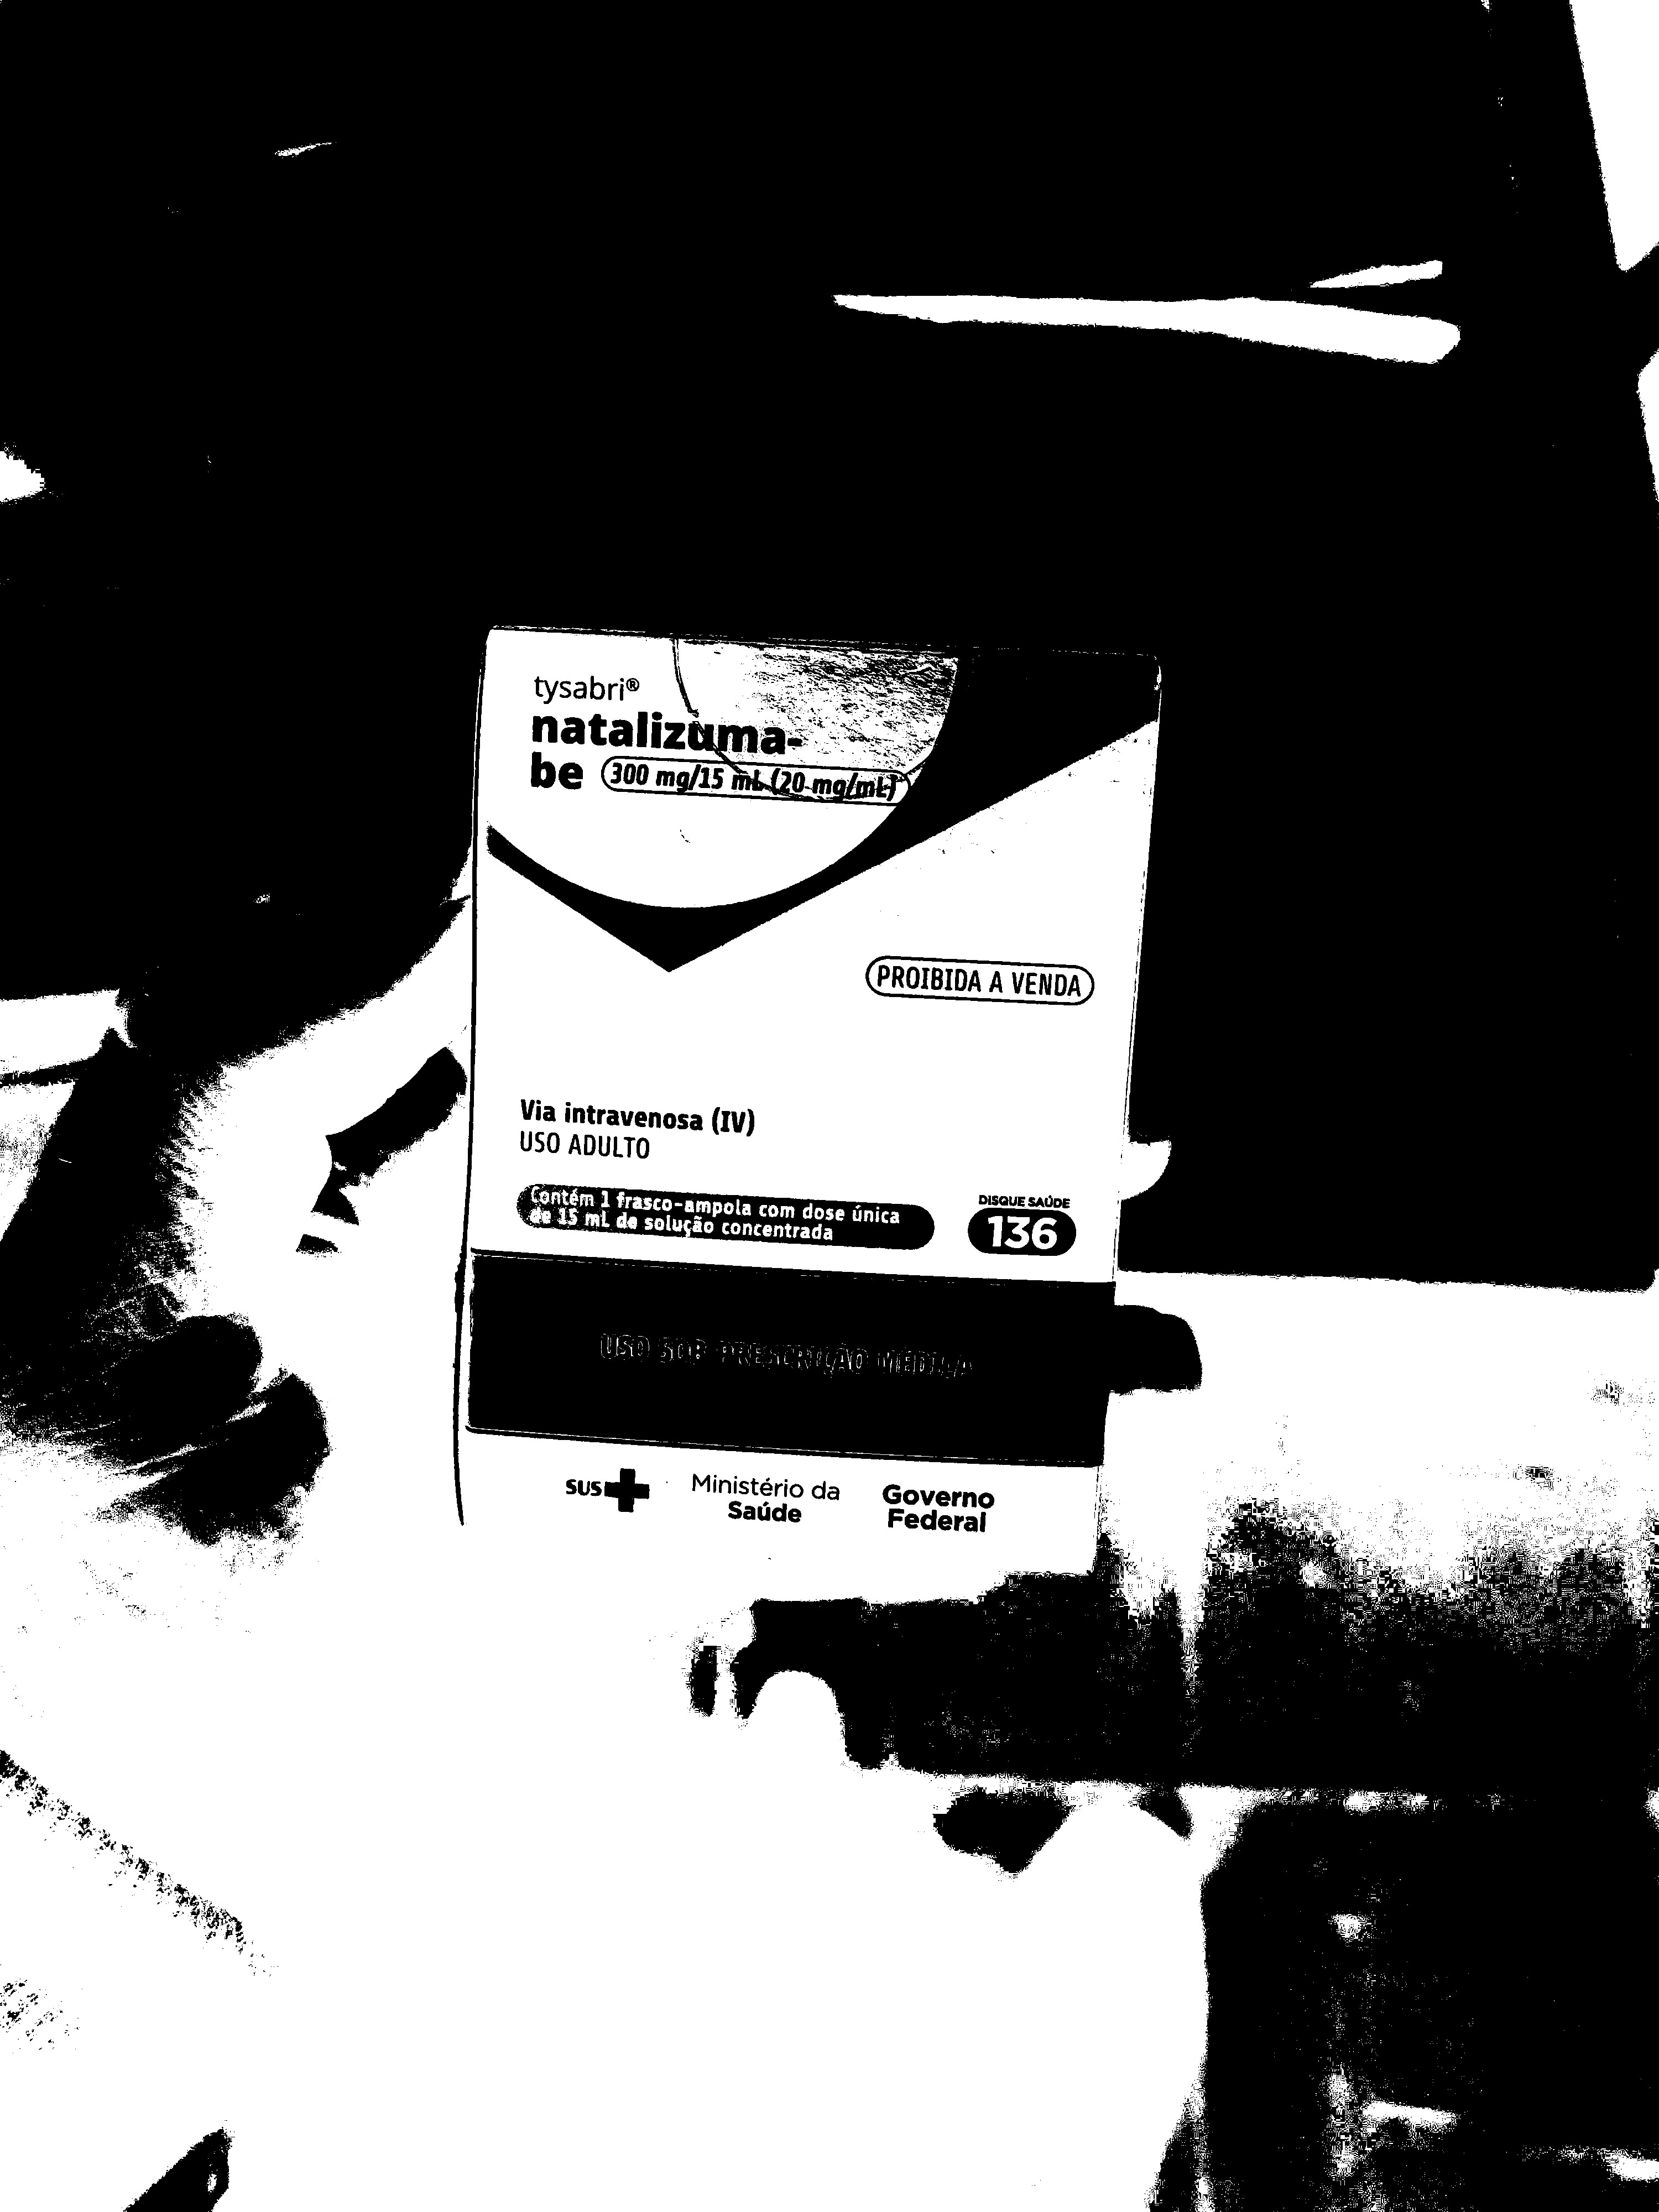
\includegraphics[width=\linewidth]{../pictures/tysabri_cmyk_k_only_thresh.jpg}
    \end{subfigure}
    \\\vspace{\floatsep}
    \begin{subfigure}[t]{0.21\textwidth}
        \centering
        \caption{C thresh.}
        \label{fig:foto:versoes:2:C_thresh:boxes}
        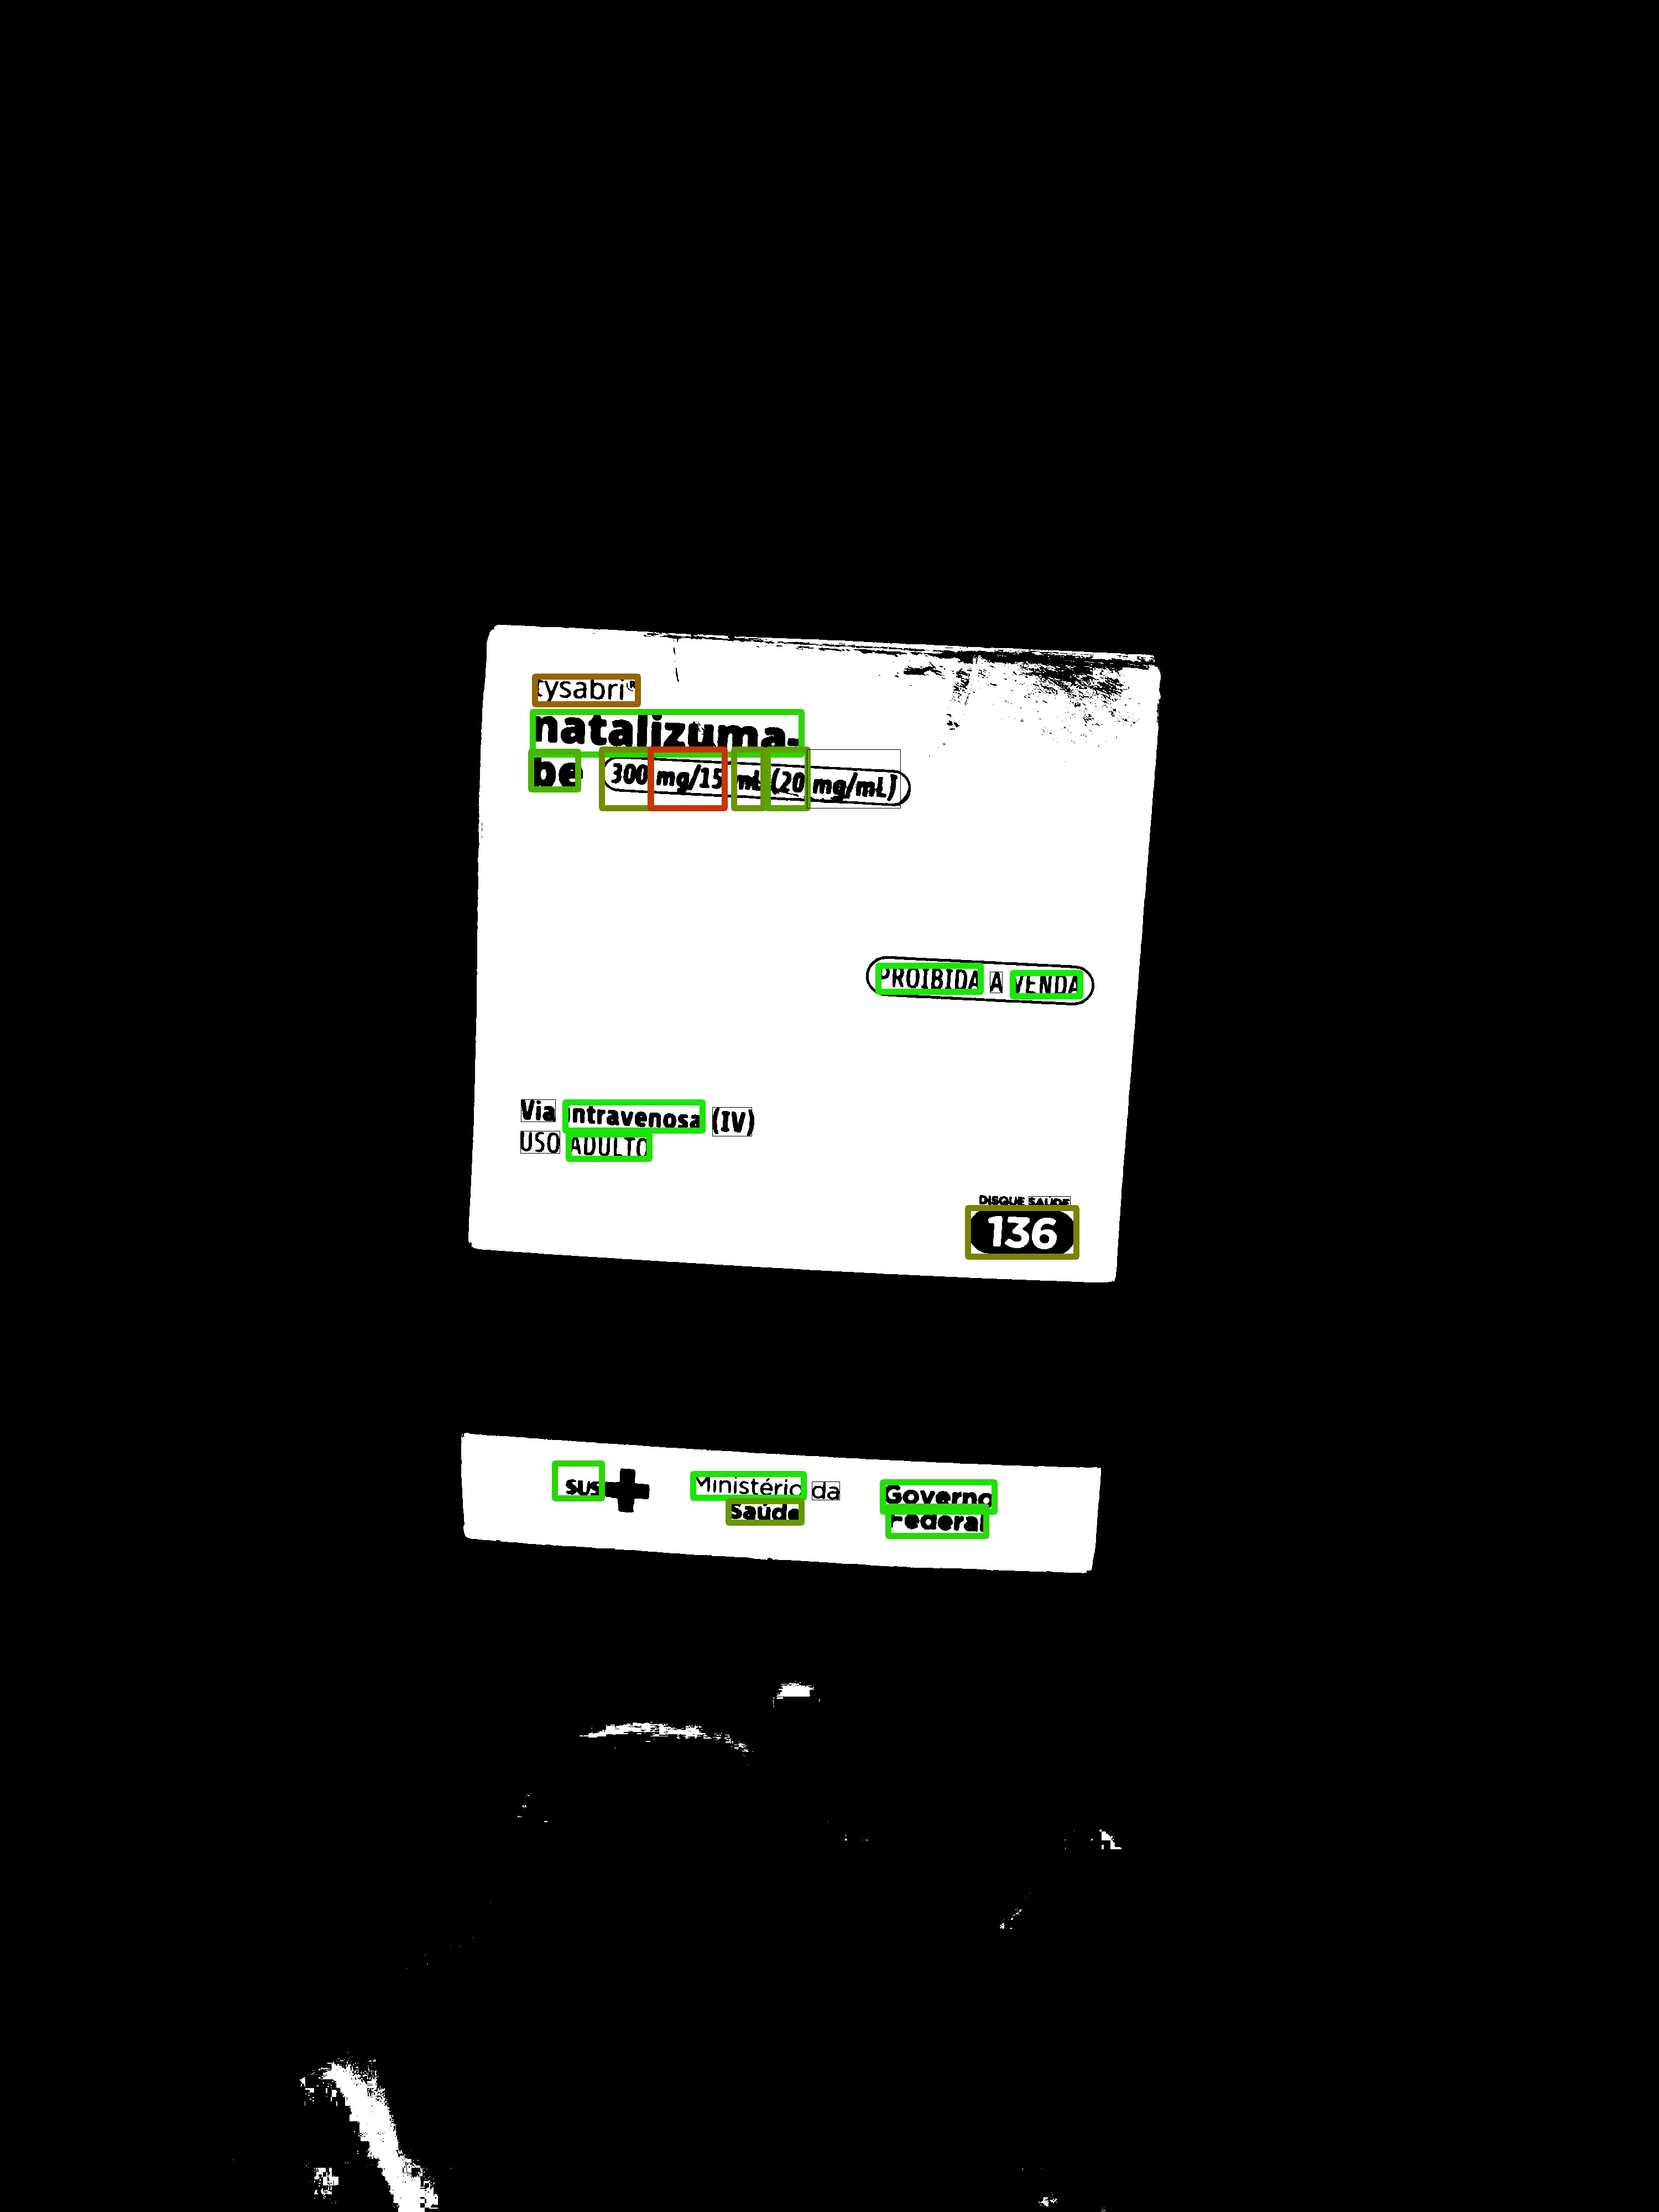
\includegraphics[width=\linewidth]{../pictures/tysabri_cmyk_c_only_thresh_boxes.jpg}
    \end{subfigure}
    \hfill
    \begin{subfigure}[t]{0.21\textwidth}
        \centering
        \caption{M thresh.}
        \label{fig:foto:versoes:2:M_thresh:boxes}
        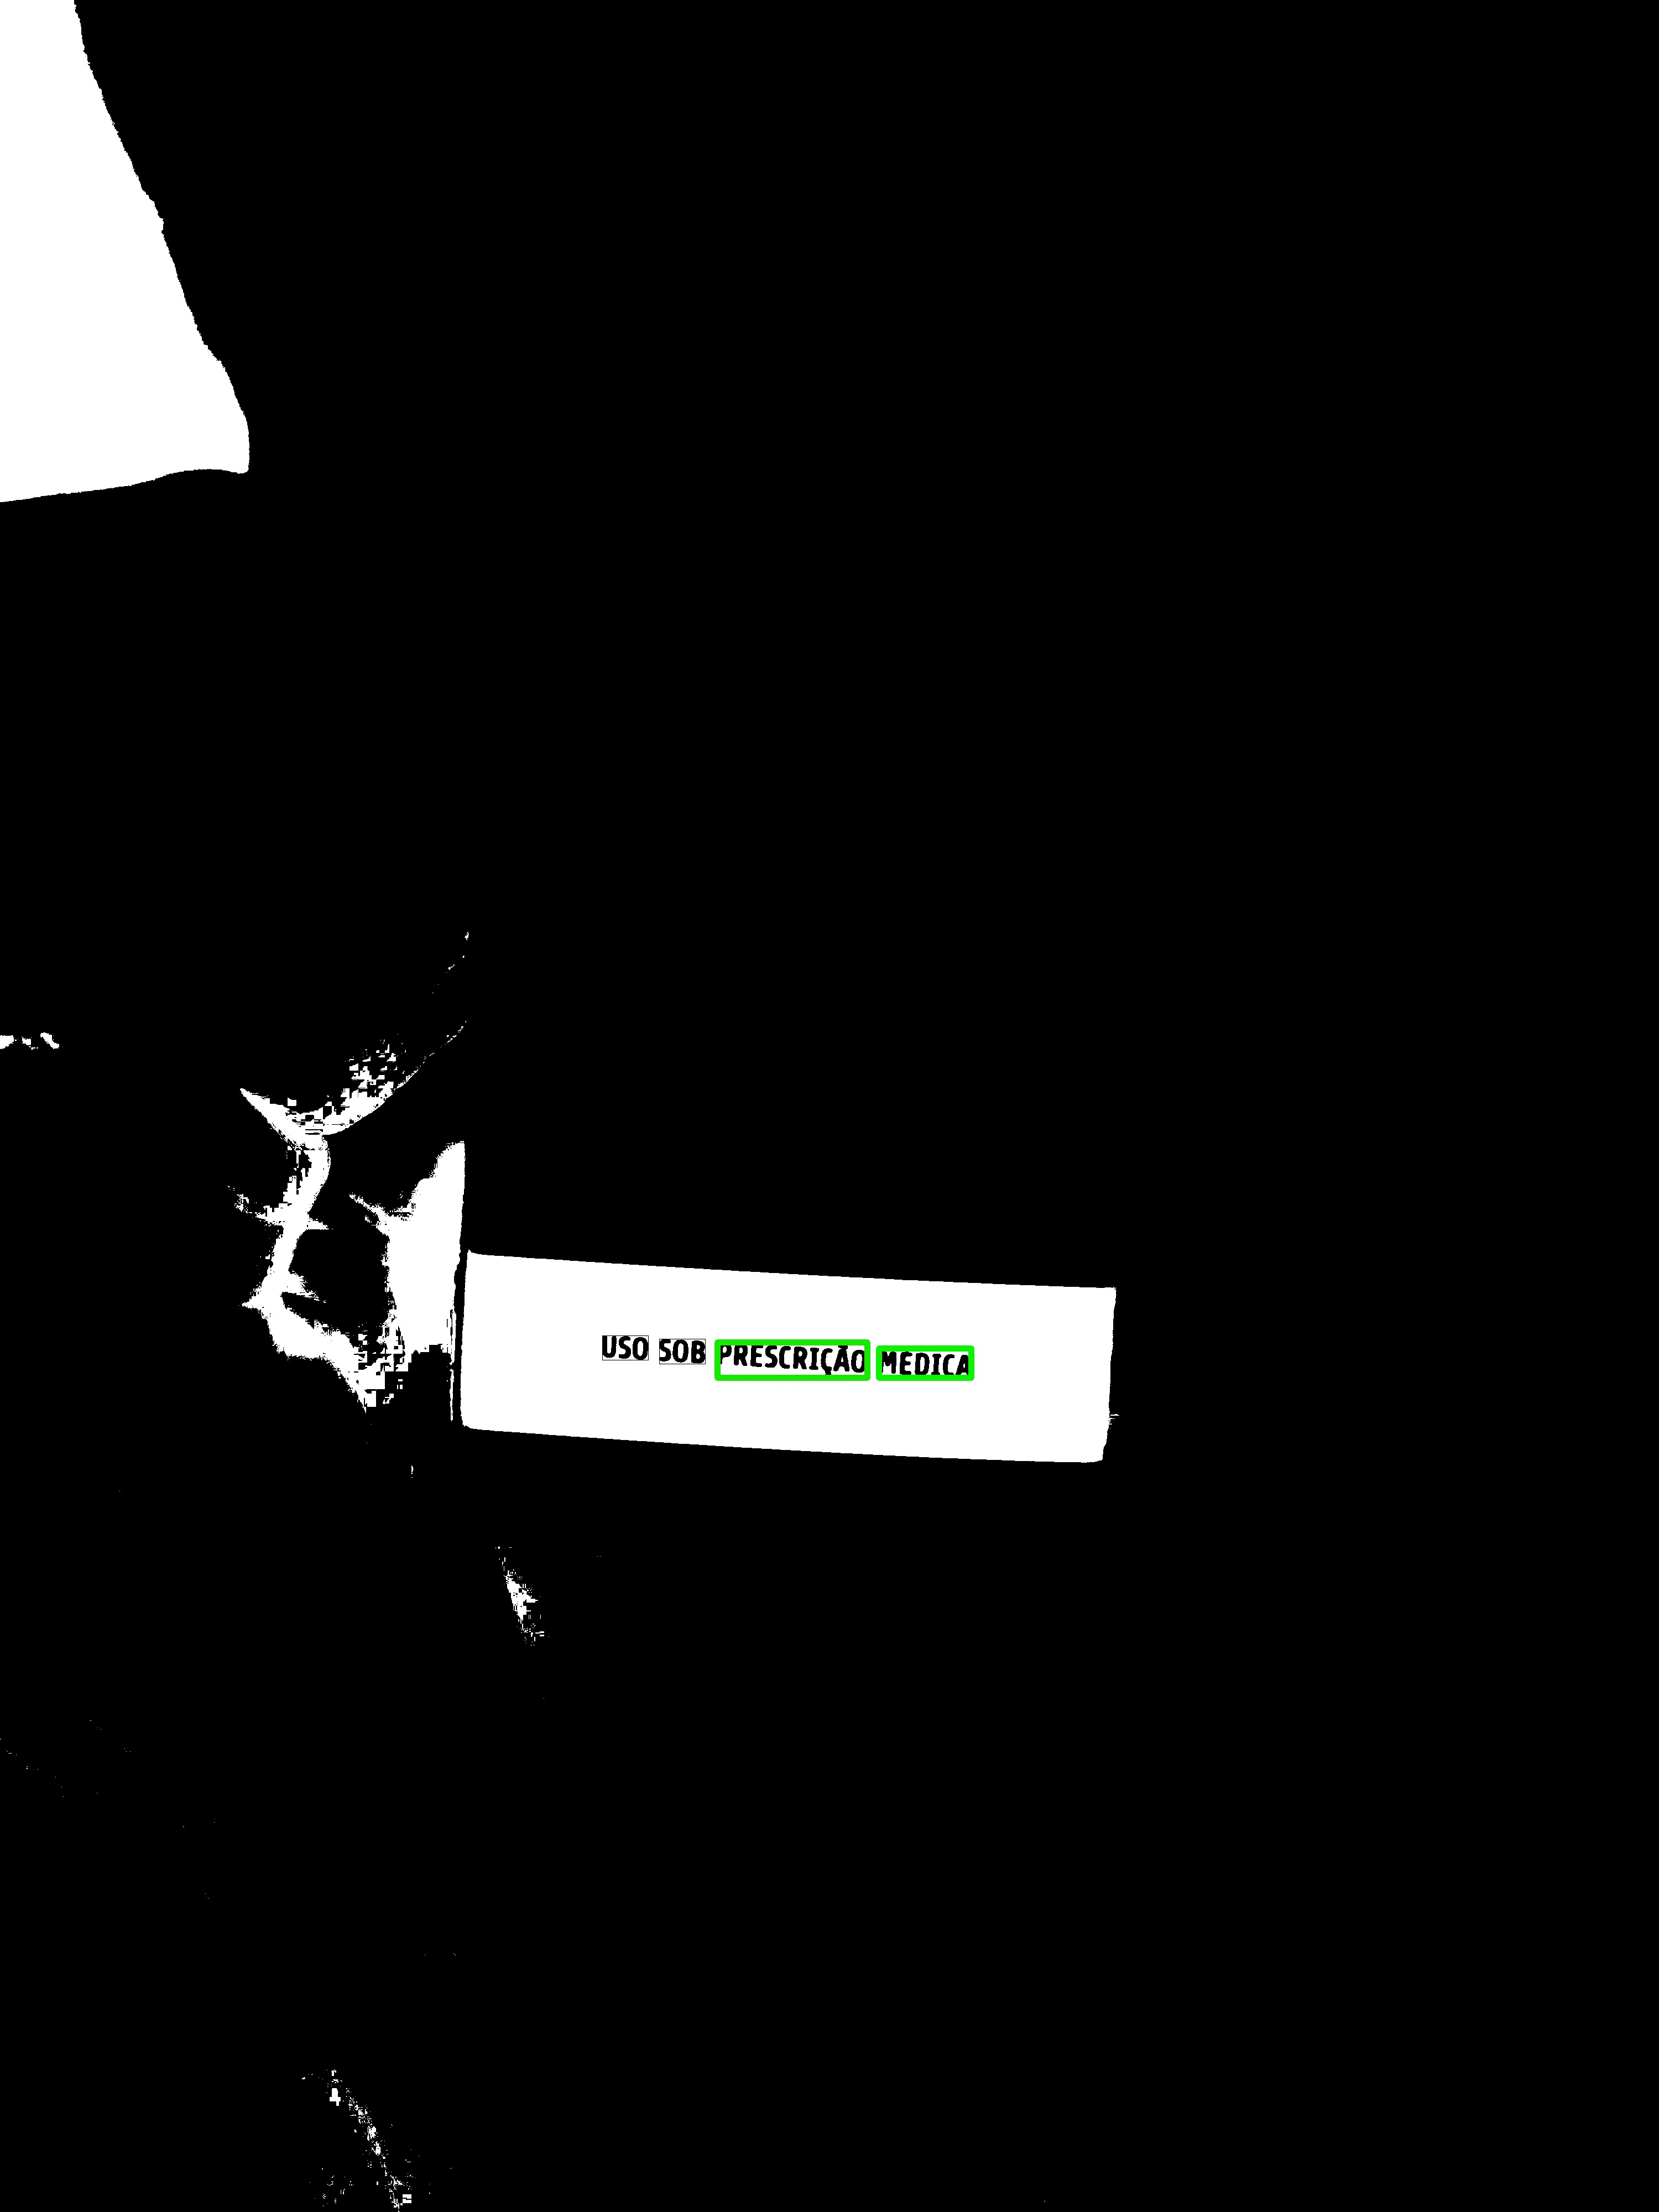
\includegraphics[width=\linewidth]{../pictures/tysabri_cmyk_m_only_thresh_boxes.jpg}
    \end{subfigure}
    \hfill
    \begin{subfigure}[t]{0.21\textwidth}
        \centering
        \caption{Y thresh.}
        \label{fig:foto:versoes:2:Y_thresh:boxes}
        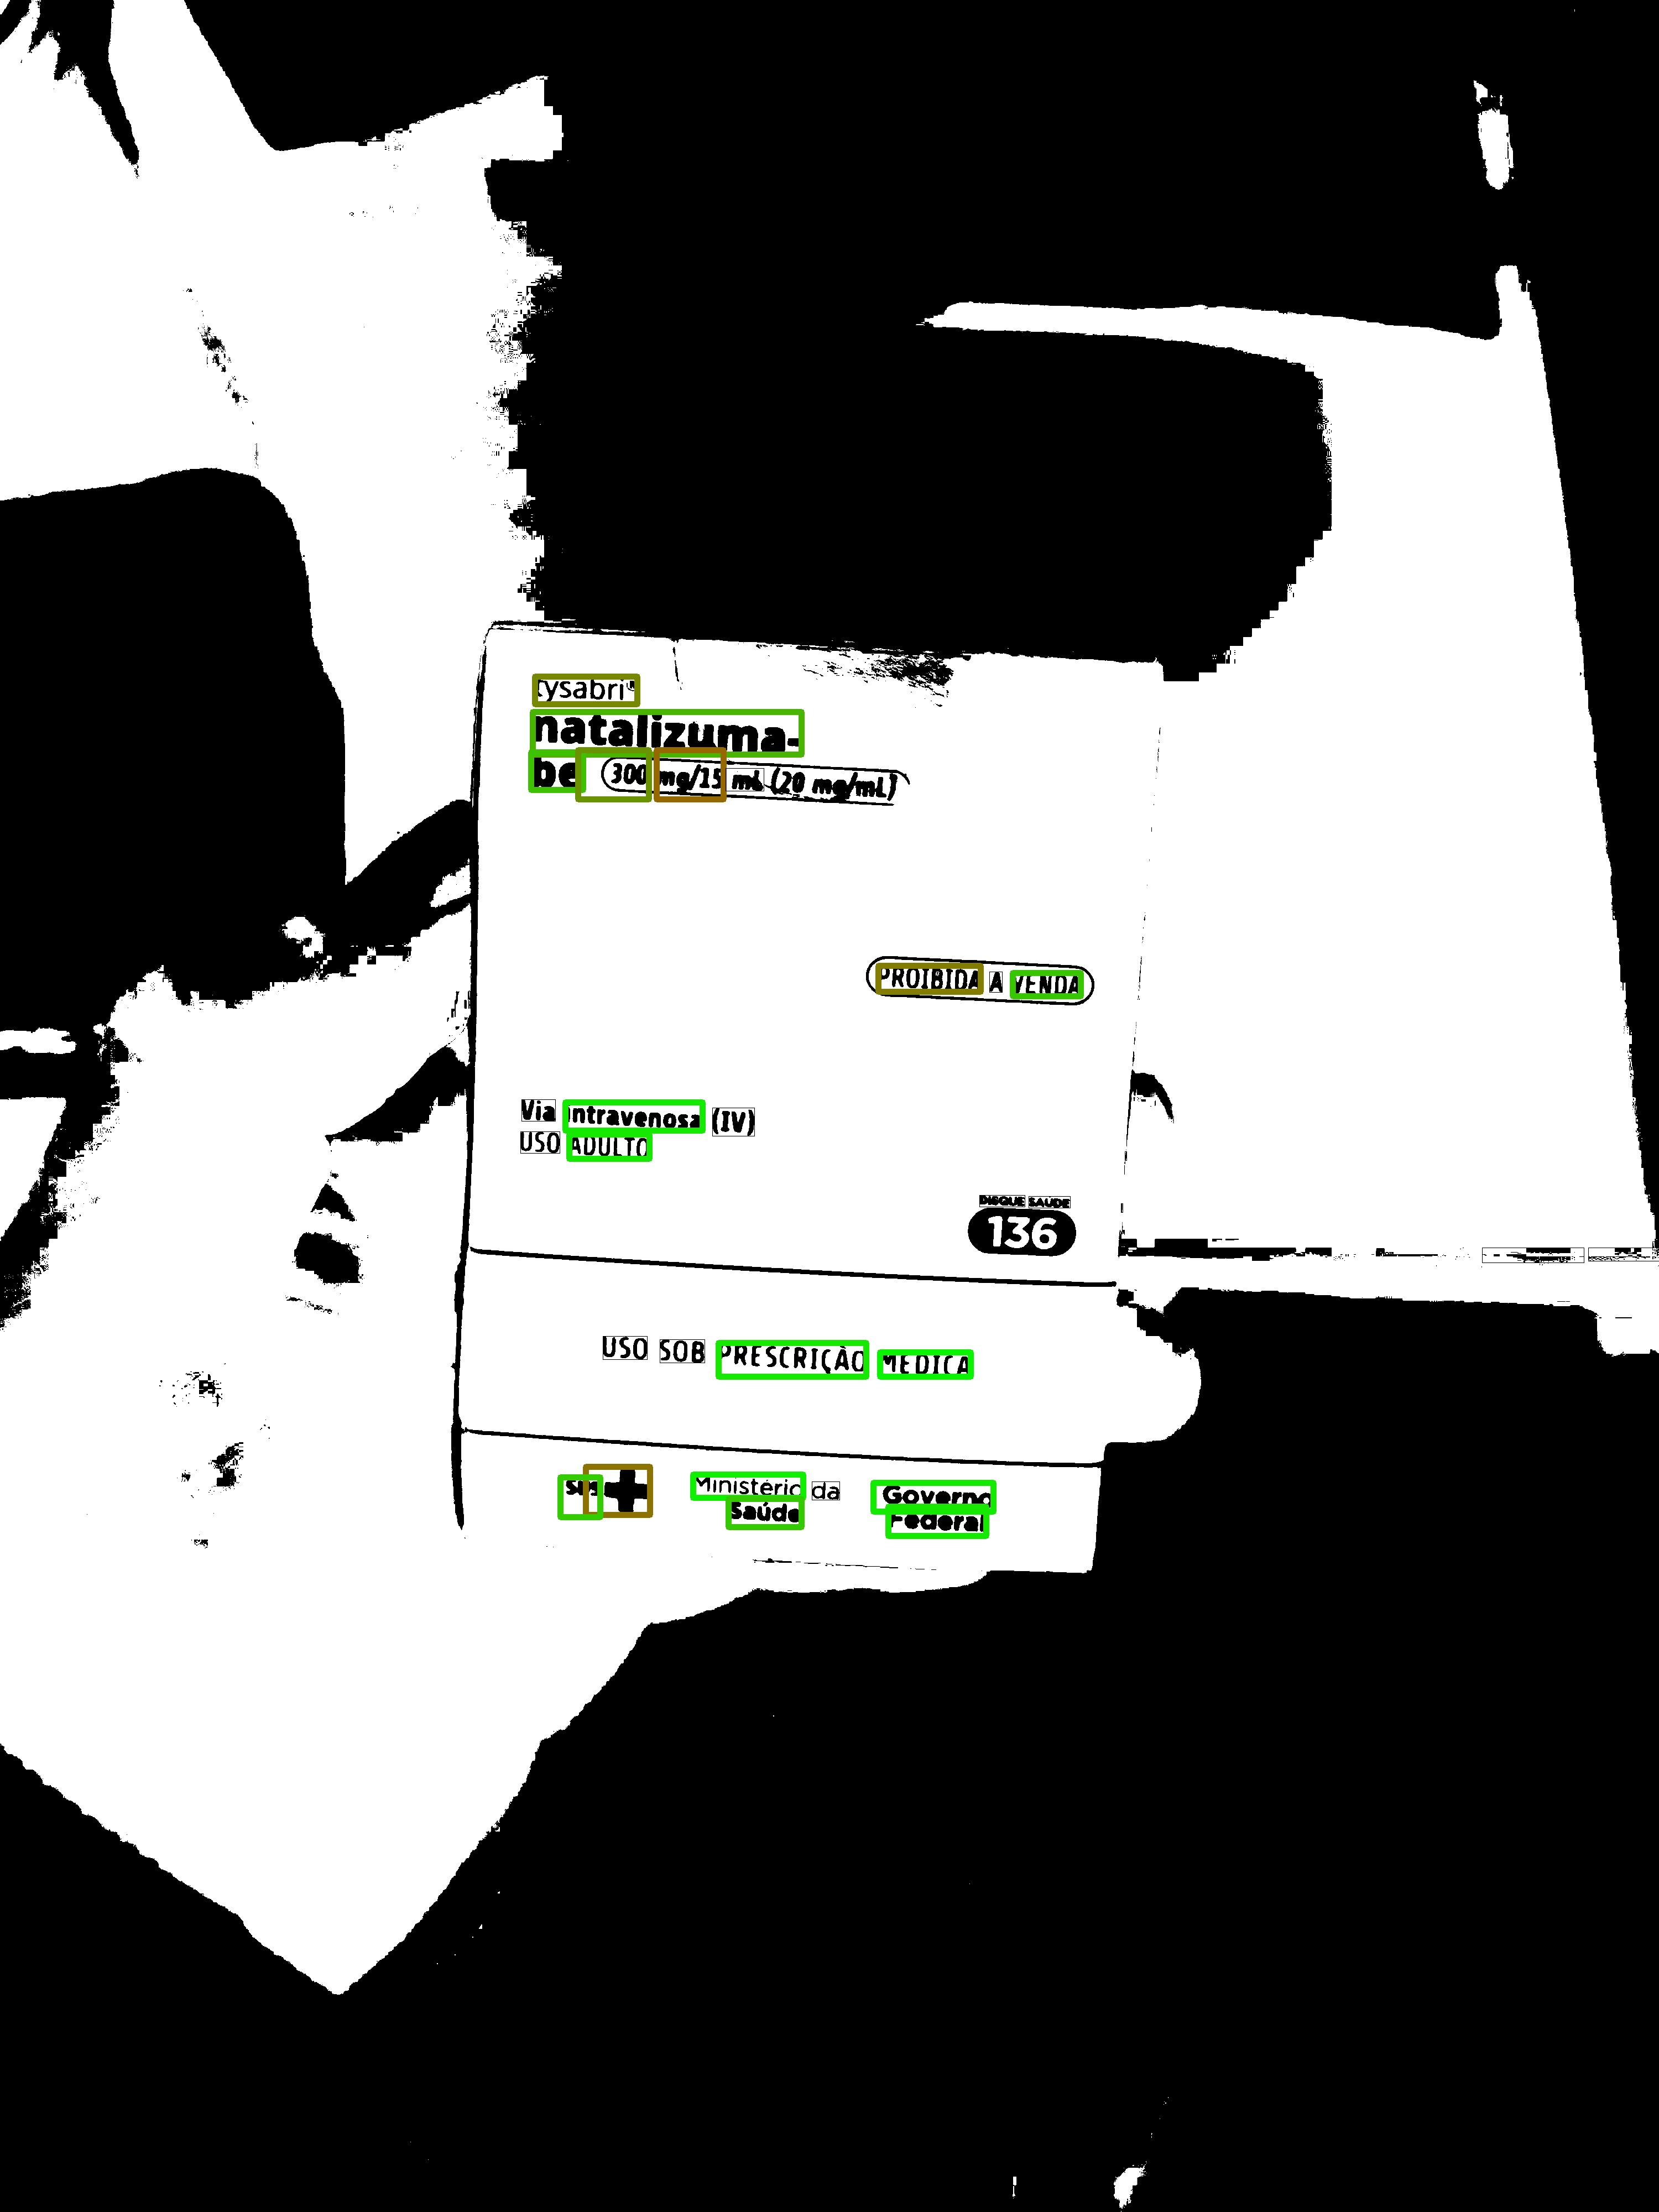
\includegraphics[width=\linewidth]{../pictures/tysabri_cmyk_y_only_thresh_boxes.jpg}
    \end{subfigure}
    \hfill
    \begin{subfigure}[t]{0.21\textwidth}
        \centering
        \caption{K thresh.}
        \label{fig:foto:versoes:2:K_thresh:boxes}
        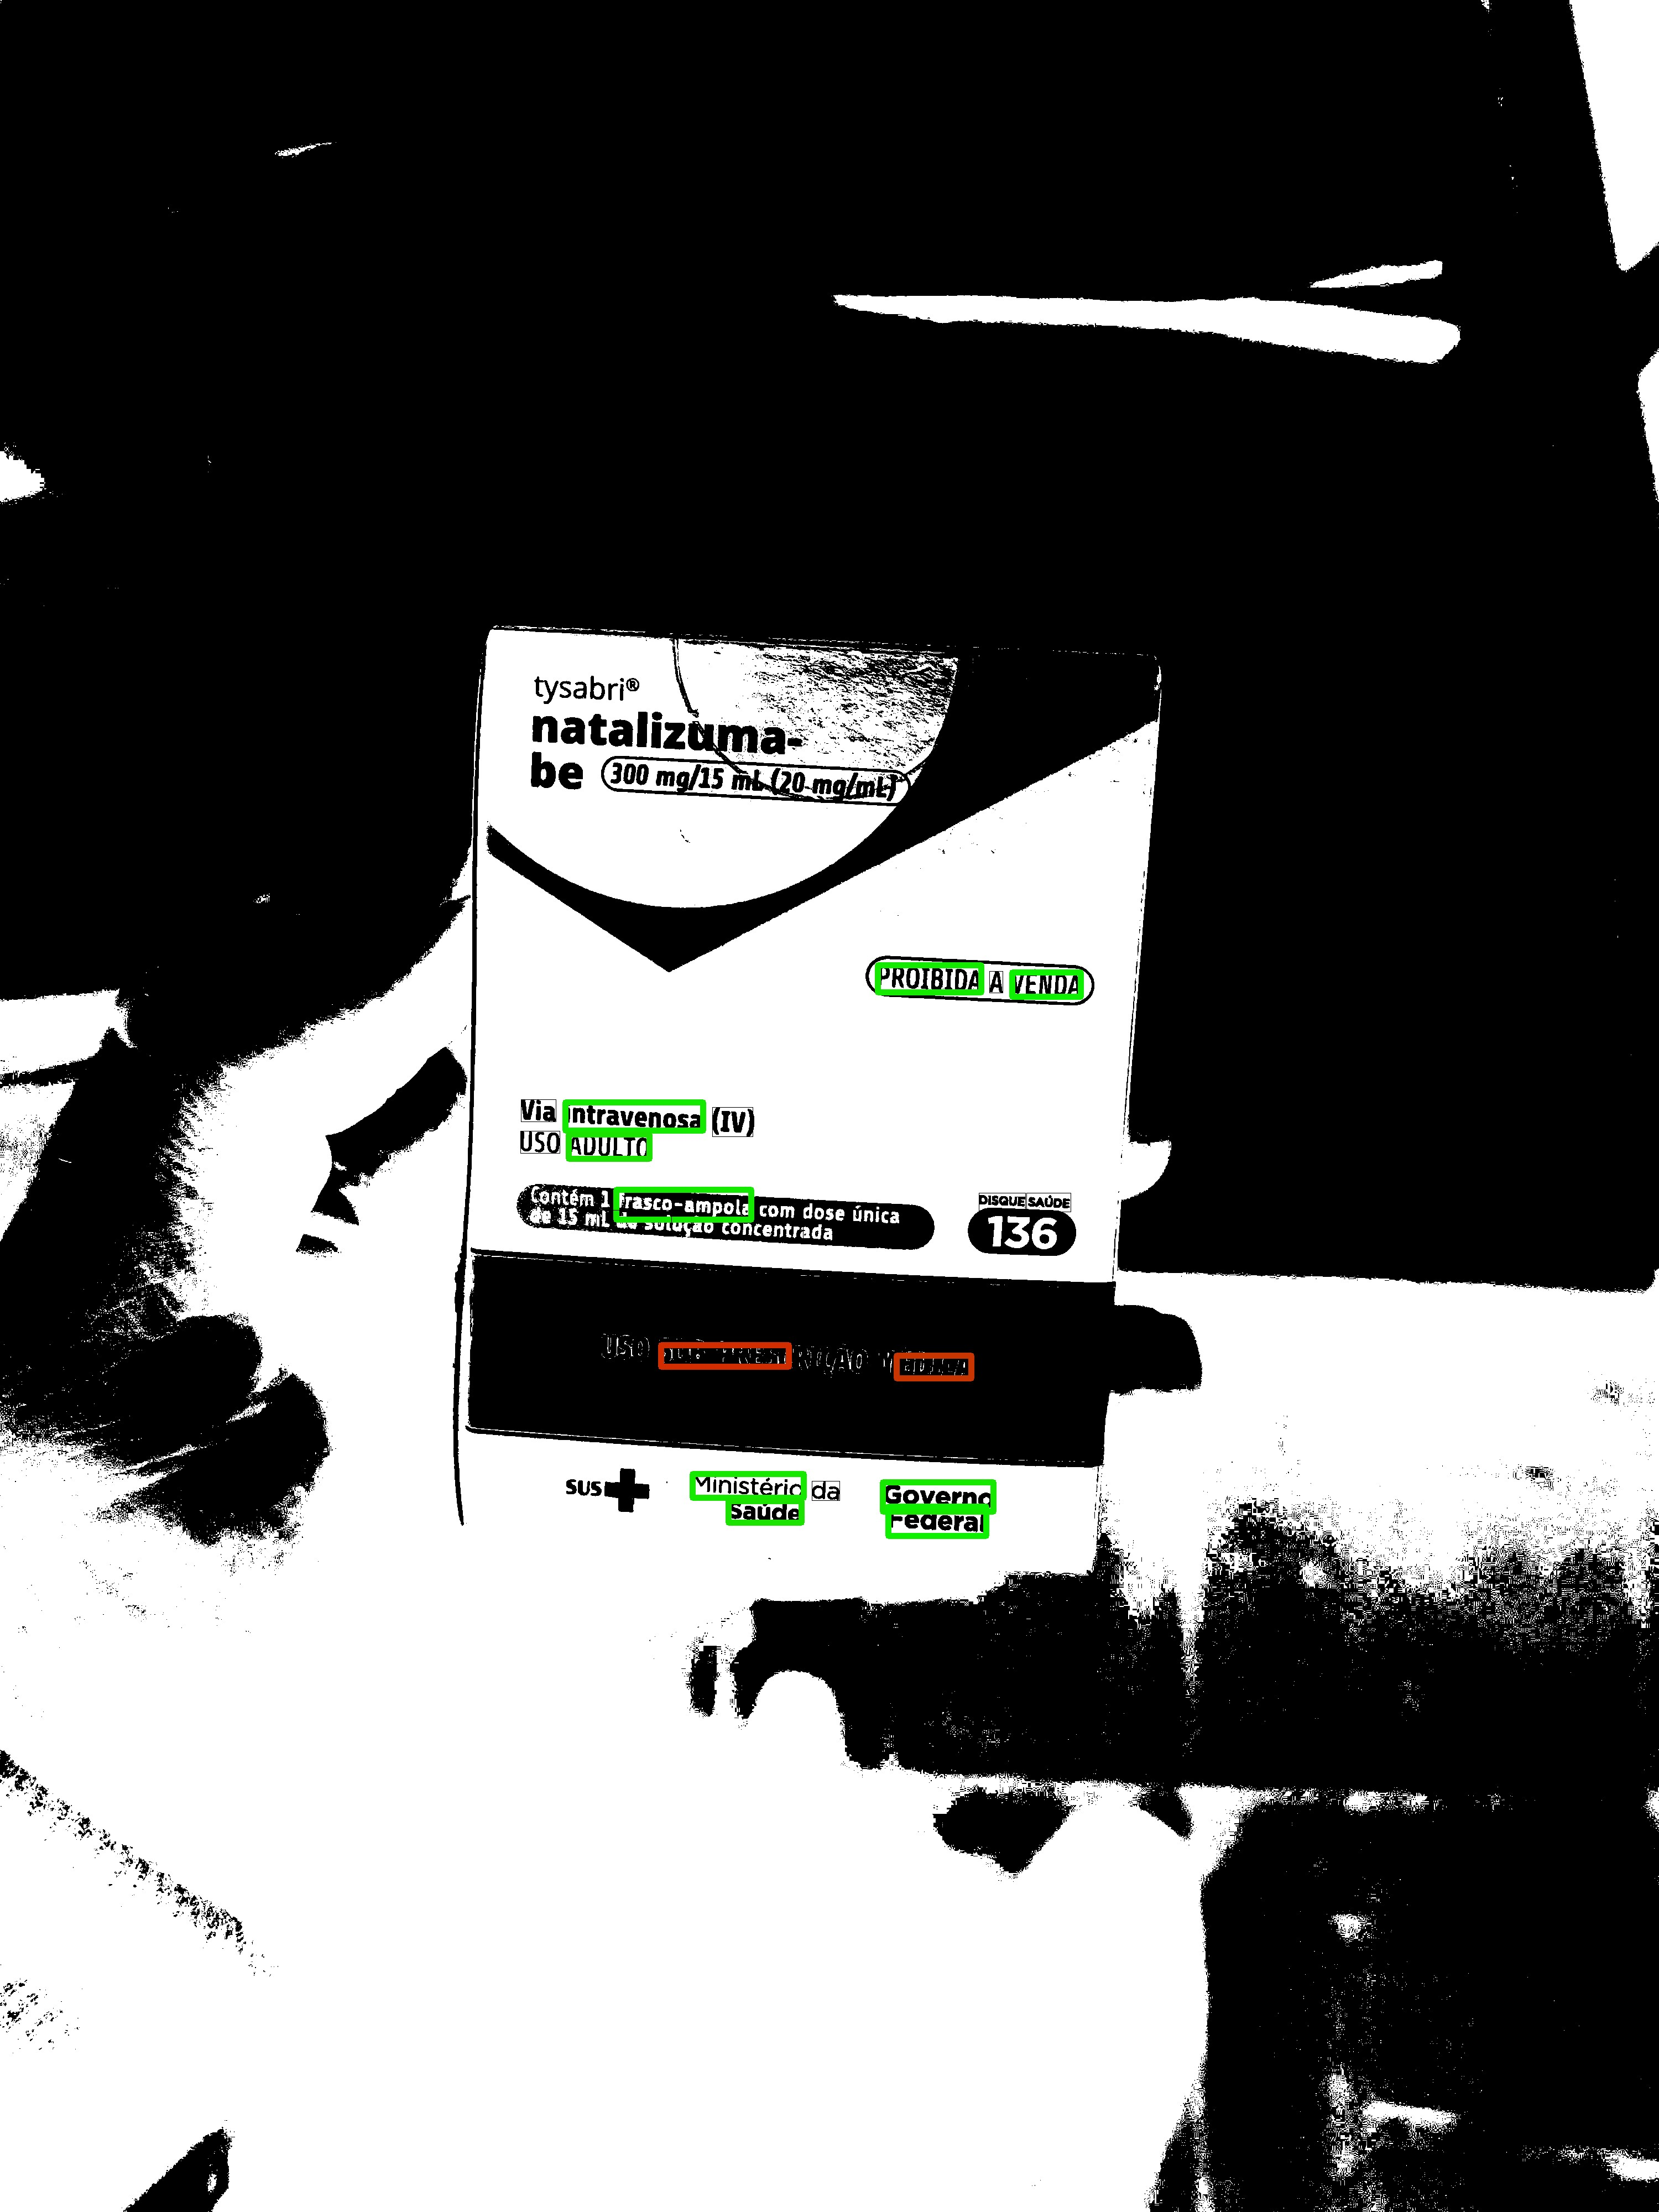
\includegraphics[width=\linewidth]{../pictures/tysabri_cmyk_k_only_thresh_boxes.jpg}
    \end{subfigure}
    \caption*{Fonte: Autor.}
    \label{fig:foto:versoes:2}
\end{figure}

















\begin{figure}[htb]
    \centering
    \caption{Exemplos de componentes analisadas recompondo componentes de \textit{threshold} (%
    \subref{fig:foto:versoes:2:RGB},
    \subref{fig:foto:versoes:2:RGB_Cinza},
    \subref{fig:foto:versoes:2:CMYK},
    \subref{fig:foto:versoes:2:RGB_CMYK}%
    ) e destaque nos termos localizados em cada componente (%
    \subref{fig:foto:versoes:2:RGB:boxes},
    \subref{fig:foto:versoes:2:RGB_Cinza:boxes},
    \subref{fig:foto:versoes:2:CMYK:boxes},
    \subref{fig:foto:versoes:2:RGB_CMYK:boxes}%
    ).}
    % \hfill
    \begin{subfigure}[b]{0.21\textwidth}
        \centering
        \caption{RGB.}
        \label{fig:foto:versoes:2:RGB}
        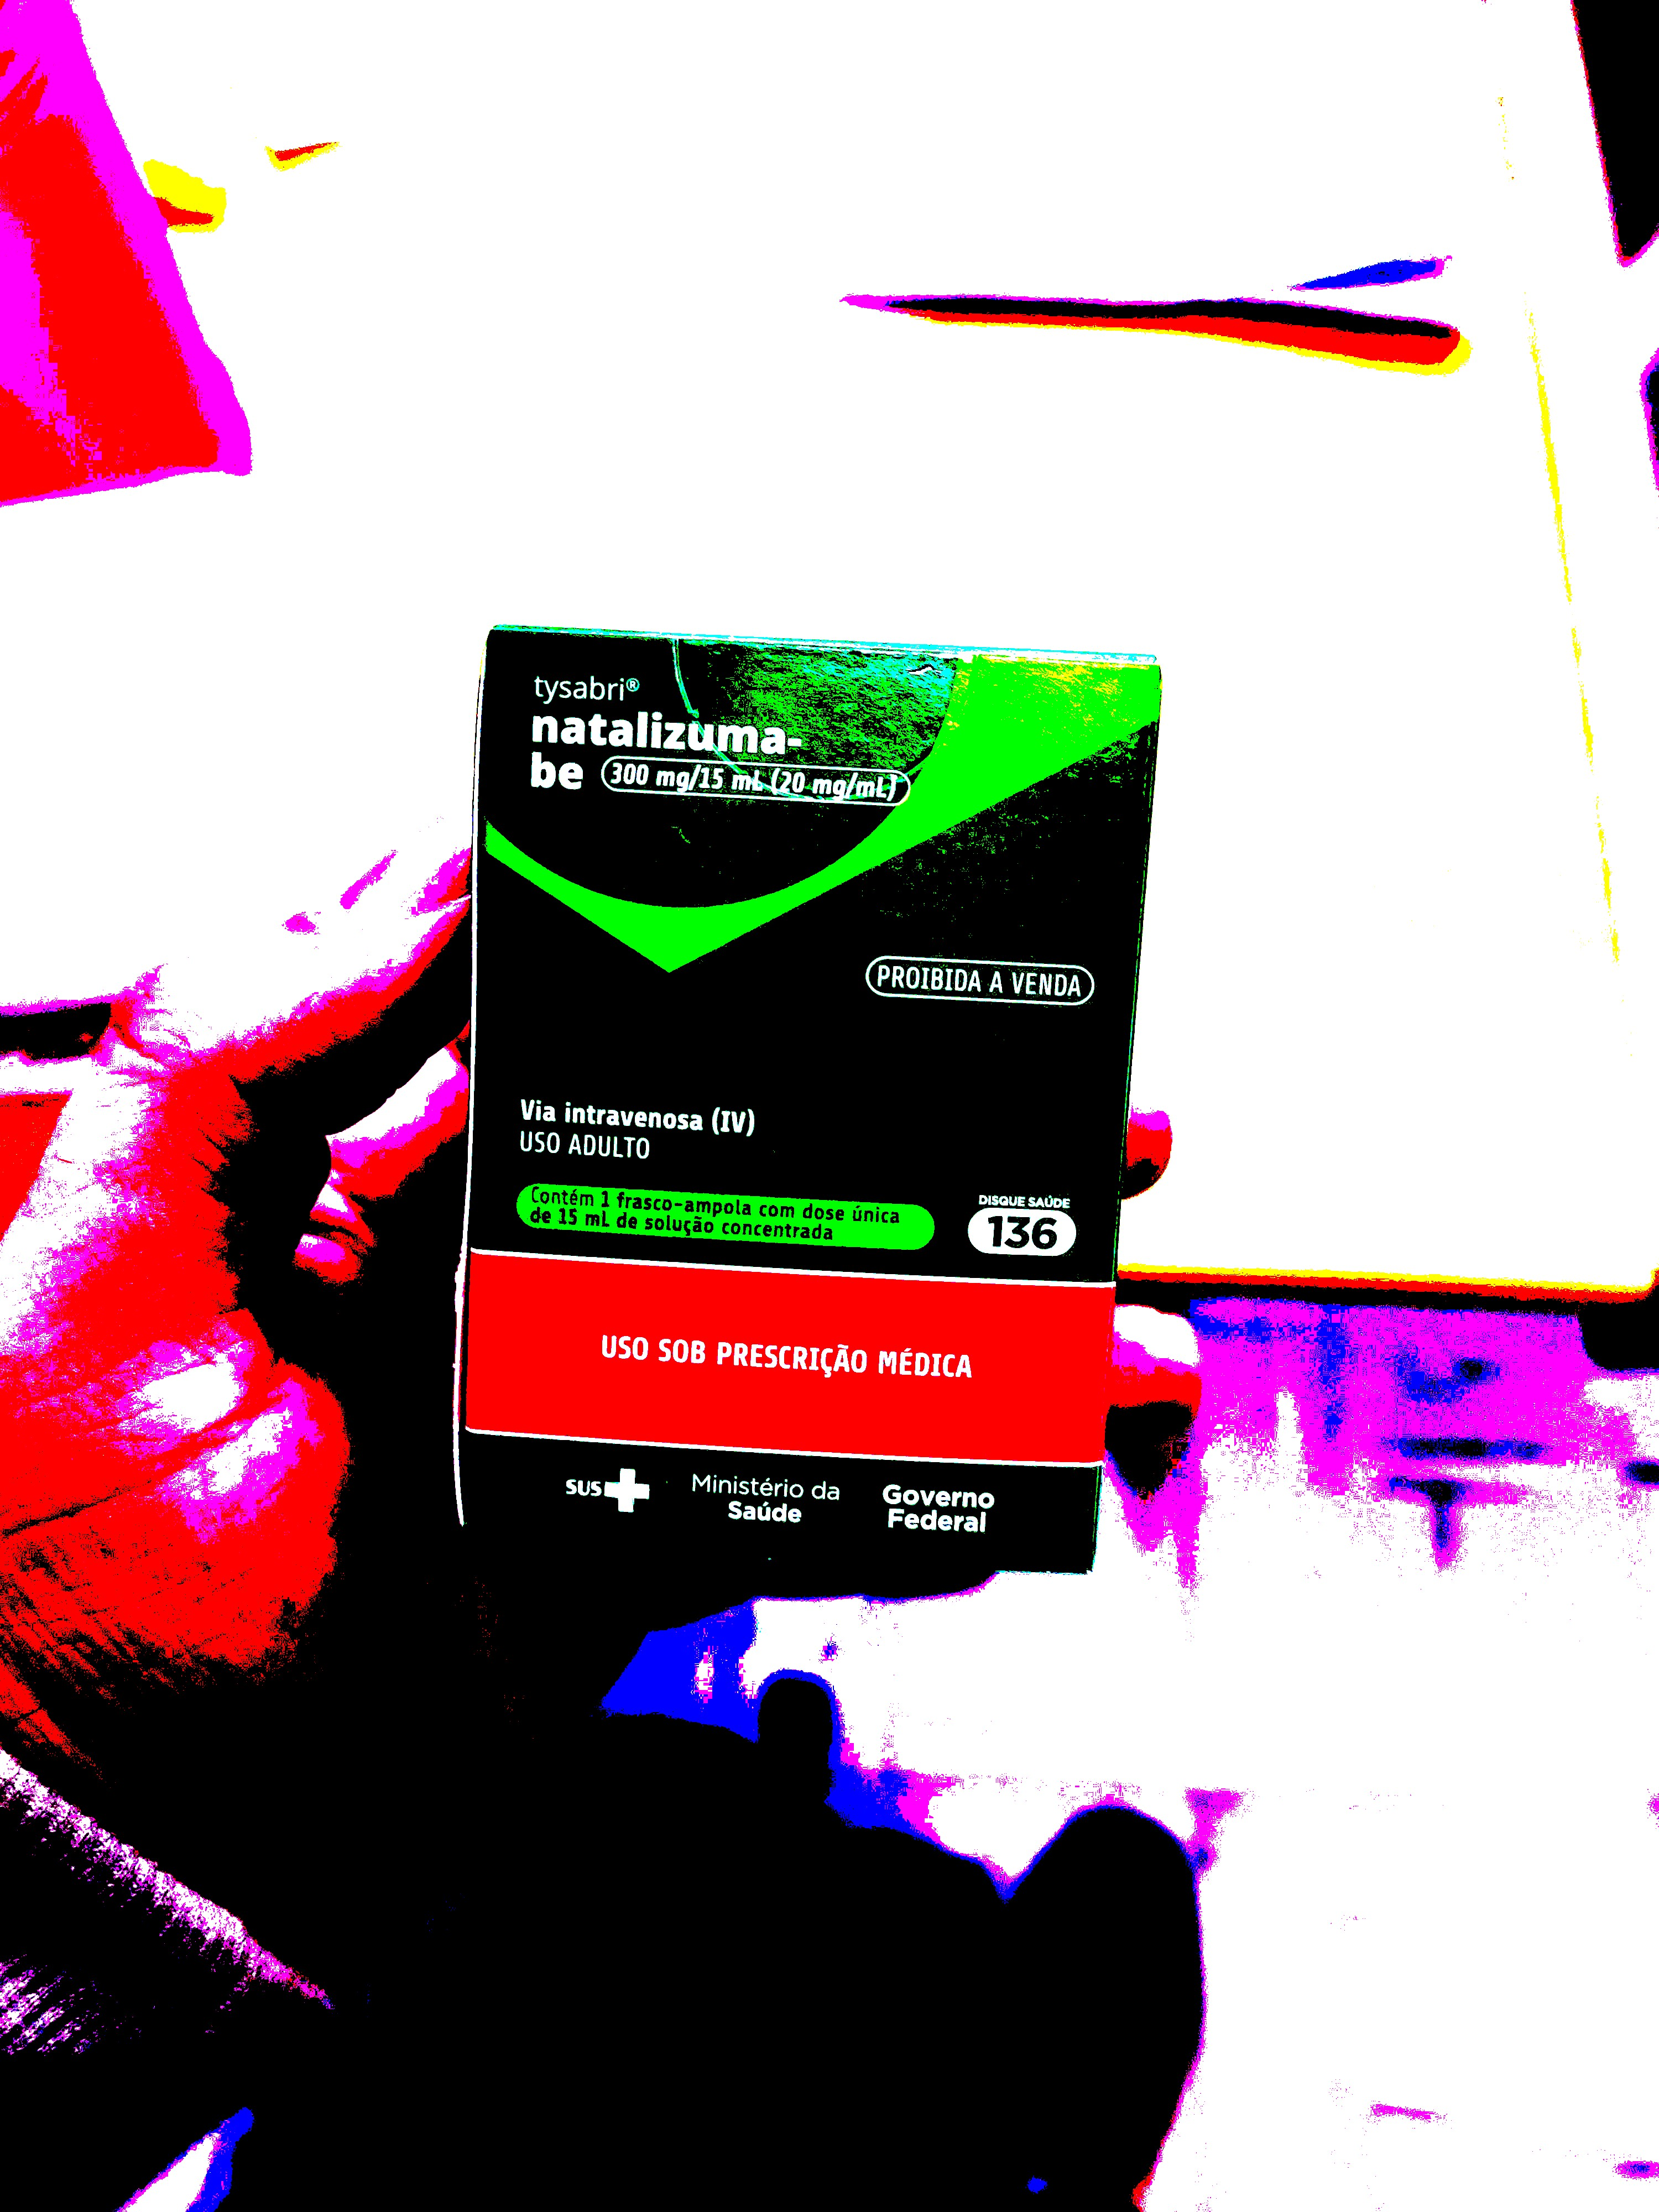
\includegraphics[width=\linewidth]{../pictures/tysabri_rgb_thresh.jpg}
    \end{subfigure}
    \hfill
    \begin{subfigure}[b]{0.21\textwidth}
        \centering
        \caption{RGB Cinza.}
        \label{fig:foto:versoes:2:RGB_Cinza}
        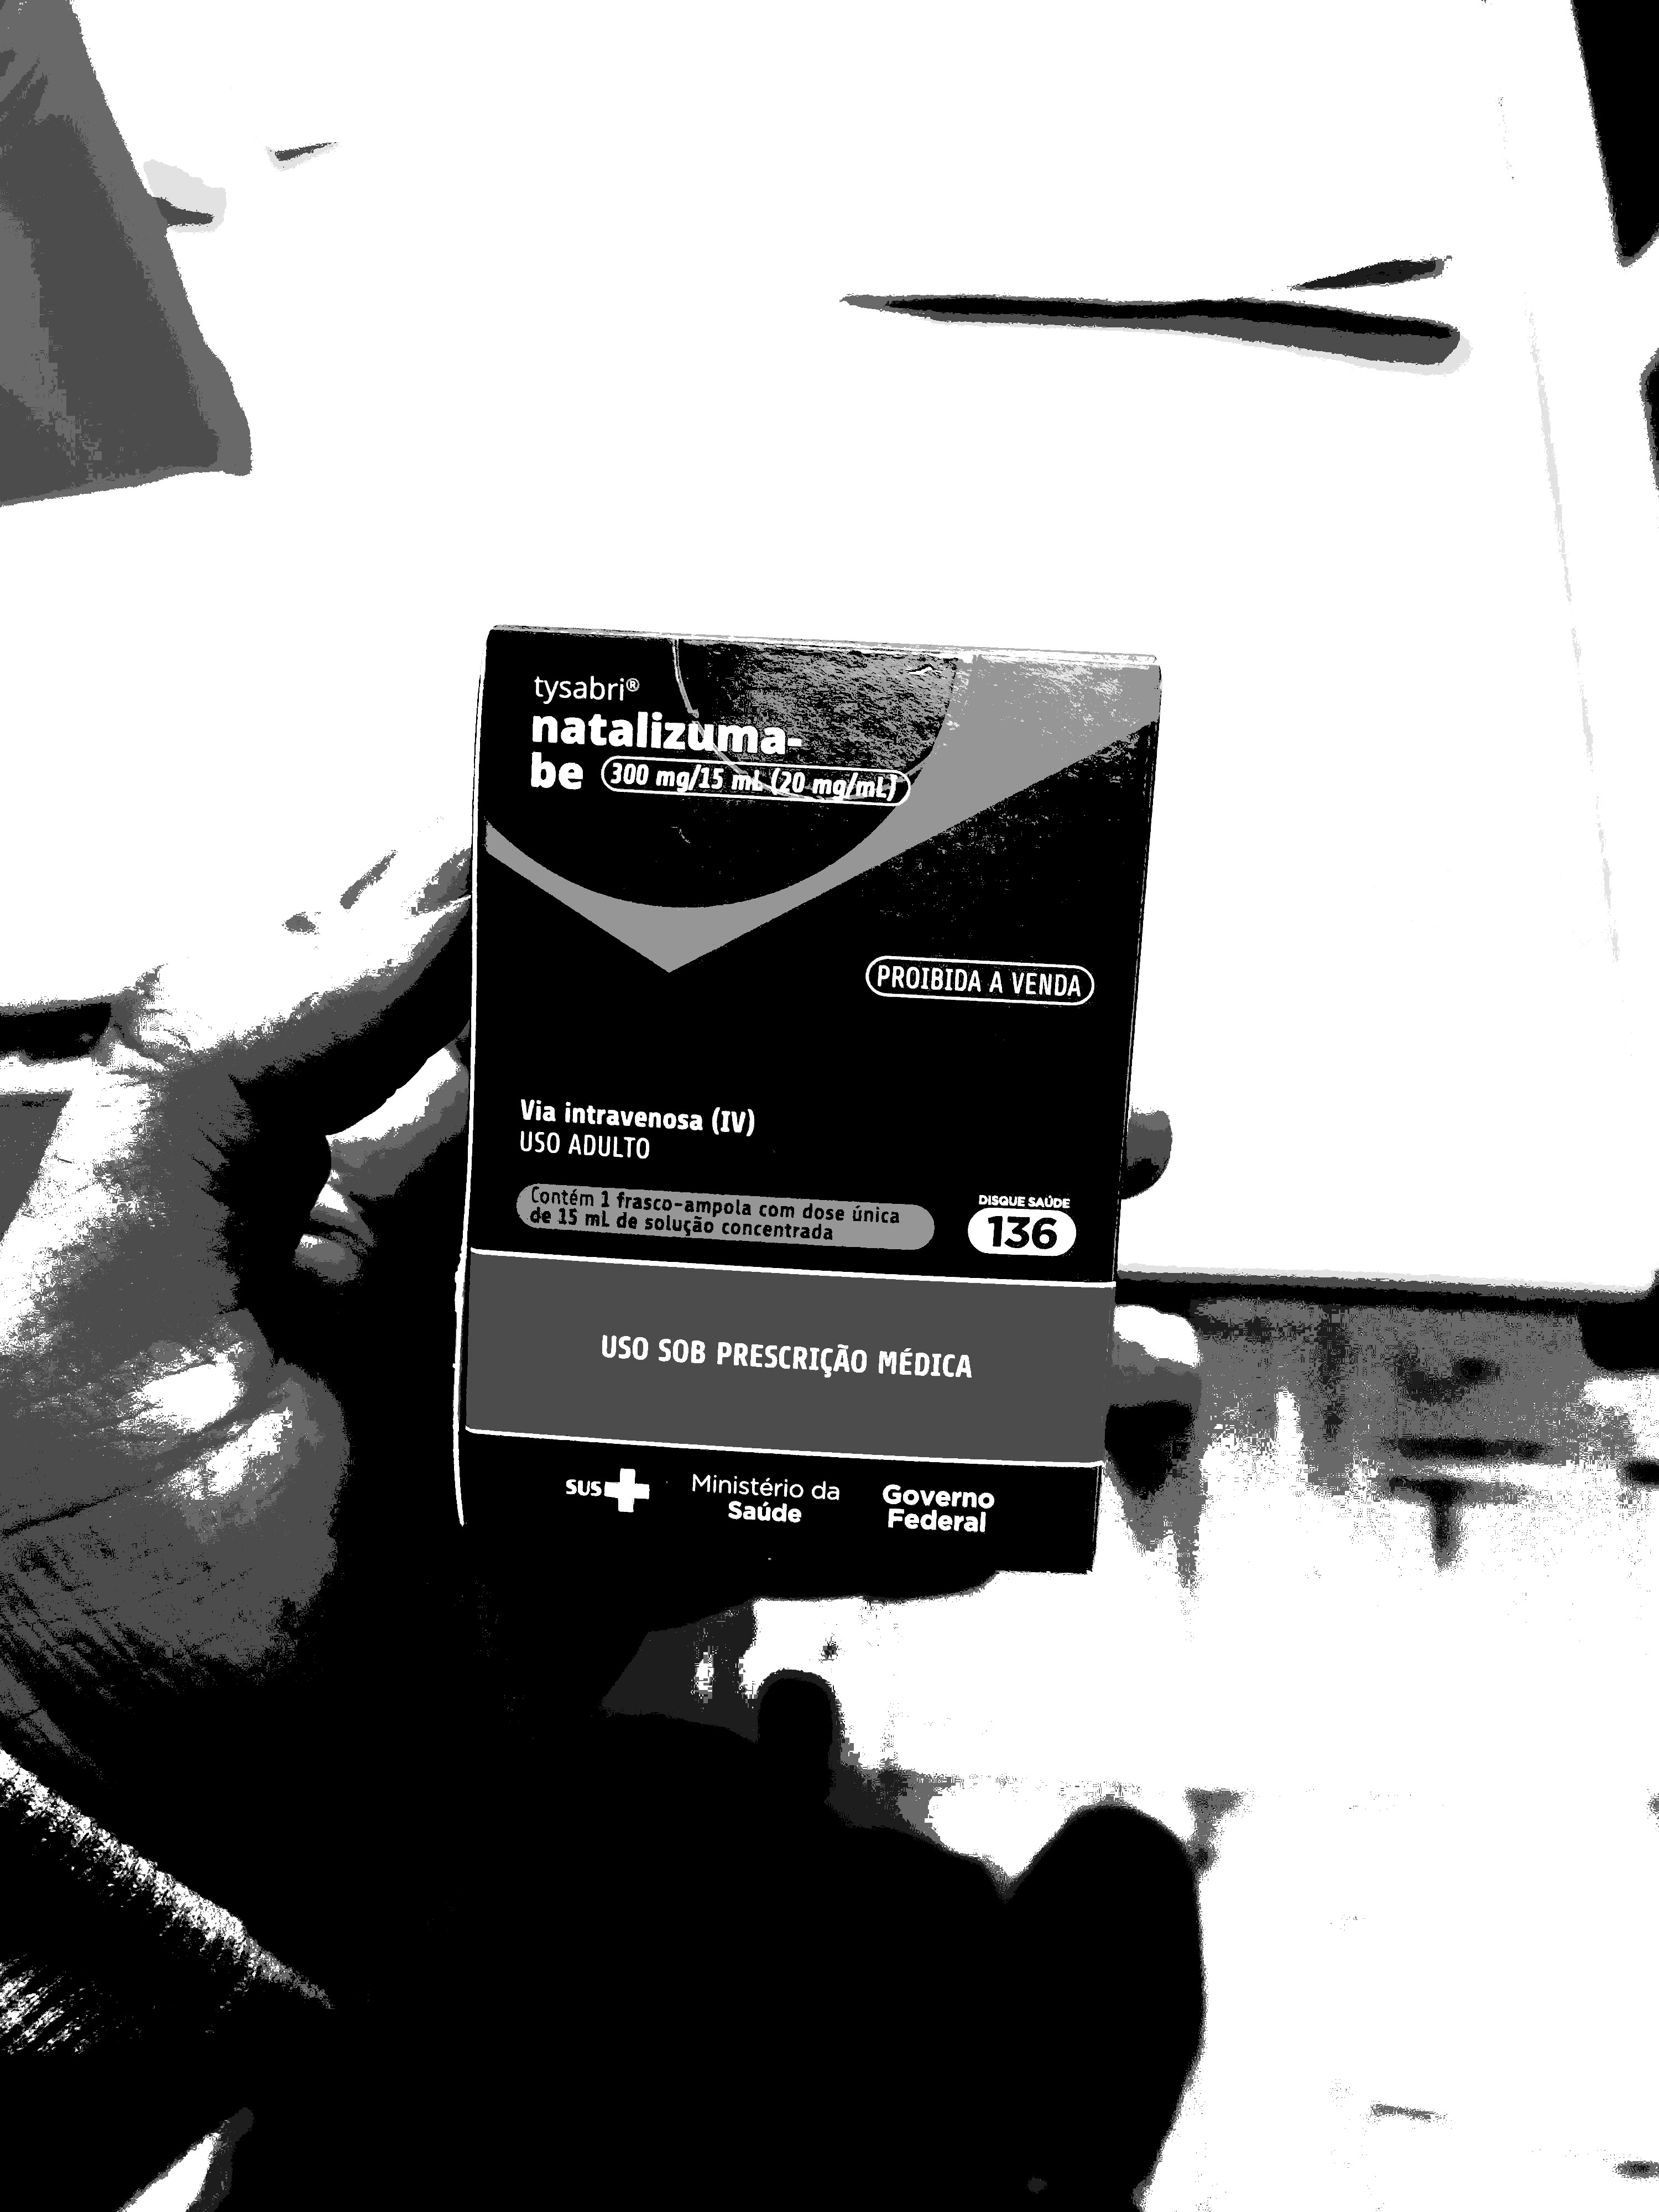
\includegraphics[width=\linewidth]{../pictures/tysabri_rgb_thresh_gray_thresh.jpg}
    \end{subfigure}
    \hfill
    \begin{subfigure}[b]{0.21\textwidth}
        \centering
        \caption{CMYK.}
        \label{fig:foto:versoes:2:CMYK}
        \includegraphics[width=\linewidth]{../pictures/tysabri_cmyk_thresh.jpg}
    \end{subfigure}
    \hfill
    \begin{subfigure}[b]{0.21\textwidth}
        \centering
        \caption{RGB CMYK.}
        \label{fig:foto:versoes:2:RGB_CMYK}
        \includegraphics[width=\linewidth]{../pictures/tysabri_rgb_thresh_recomposed_cmyk.jpg}
    \end{subfigure}
    \\\vspace{\floatsep}
    \begin{subfigure}[b]{0.21\textwidth}
        \centering
        \caption{RGB.}
        \label{fig:foto:versoes:2:RGB:boxes}
        \includegraphics[width=\linewidth]{../pictures/tysabri_rgb_thresh_boxes.jpg}
    \end{subfigure}
    \hfill
    \begin{subfigure}[b]{0.21\textwidth}
        \centering
        \caption{RGB Cinza.}
        \label{fig:foto:versoes:2:RGB_Cinza:boxes}
        \includegraphics[width=\linewidth]{../pictures/tysabri_rgb_thresh_gray_thresh_boxes.jpg}
    \end{subfigure}
    \hfill
    \begin{subfigure}[b]{0.21\textwidth}
        \centering
        \caption{CMYK.}
        \label{fig:foto:versoes:2:CMYK:boxes}
        \includegraphics[width=\linewidth]{../pictures/tysabri_cmyk_thresh_boxes.jpg}
    \end{subfigure}
    \hfill
    \begin{subfigure}[b]{0.21\textwidth}
        \centering
        \caption{RGB CMYK.}
        \label{fig:foto:versoes:2:RGB_CMYK:boxes}
        \includegraphics[width=\linewidth]{../pictures/tysabri_rgb_thresh_recomposed_cmyk_boxes.jpg}
    \end{subfigure}
    \caption*{Fonte: Autor.}
    % \hfill
    \label{fig:foto:versoes:3}
\end{figure}

Os termos encontrados são adicionados a uma única lista, é possível que o mesmo tempo seja localizado em versões diferentes de imagem. Neste caso, é escolhida a versão com maior parâmetro de confiabilidade.

Cada termo encontrado é normalizado para evitar problemas na busca, removendo caracteres especiais e símbolos que não sejam letras dos termos.
São separados os termos compostos por mais de uma palavra, separados por hífen ou por detalhes na grafia, como letras maiúsculas dividindo palavras.

\subsection{Ordenar e selecionar termos encontrados na imagem}\label{ssec:organizar}

Com a lista de termos encontrados na imagem, analisando todas as codificações descritas anteriormente, é necessário ordenar os termos para que possam ser buscados.

Alguns termos recebem versões alternativas, pois a grafia correta pode ter sido removida na normalização dos termos.
Palavras com ``cao'', são replicadas para versões com ``ção'', casos semelhantes são realizados para ``ão'', ``cê'' e ``áci''.
A \autoref{fig:fotos:melagriao} apresenta um exemplo de medicamento que só é encontrado no sistema da \ac{Anvisa} se buscado com a grafia correta.
O \autoref{cod:organiza} apresenta uma simplificação da estrutura responsável por corrigir os termos.

\begin{figure}[htb]
    \centering
    \caption{Medicamento MELAGRIÃO\textsuperscript{\tiny\textregistered}, registrado na \ac{Anvisa} com caracteres especiais.}
    \label{fig:fotos:melagriao}
    \includegraphics[width=0.45\linewidth]{../pictures/melagriao.jpg}
    \caption*{Fonte: Autor.}
\end{figure}


\begin{lstfloat}[htbp]
    \centering
    \lstinputlisting[label=cod:organiza, caption={Corrigir termos, simplificado.}]{../code/ex_organizar.py}
    \caption*{Fonte: Autor.}
\end{lstfloat}

O critério de ordenação utilizado é baseado nas características dos termos da lista.
São analisadas características como a escrita do termo, as propriedades do retângulo em que o termo está inscrito e o valor de confiabilidade fornecida pelo motor de \ac{OCR}, na seguinte ordem:
\begin{enumerate}
    \item Largura do retângulo na imagem pelo cálculo da divisão inteira por 10: $\left\lfloor \sfrac{w}{10} \right\rfloor$;
    \item Quantidade de caracteres do termo;
    \item Altura do retângulo na imagem pelo calculo da divisão inteira por 10: $\left\lfloor \sfrac{h}{10} \right\rfloor$;
    \item Posição vertical do centro do retângulo;
    \item Posição horizontal do centro do retângulo;
    \item Área do retângulo  na imagem pelo calculo da divisão inteira por 1000: $\left\lfloor \sfrac{A_{\text{termo}}}{1000} \right\rfloor$;
    \item Valor de confiabilidade do termo;
    \item Ordem lexicográfica do termo;
\end{enumerate}

A ordenação da lista de termos é realizada através do método \lstinline|sort| para listas, nativo da linguagem Python \cite{pythonSorting}, utilizando uma função de comparação com os critérios apresentados anteriormente.
O \autoref{cod:organiza:2} apresenta uma simplificação da estrutura responsável por ordenar os termos encontrados.

A ordem utilizada define quais serão os primeiros termos buscados no sistema do Bulário Eletrônico da \ac{Anvisa}.

\begin{lstfloat}[htbp]
    \centering
    \lstinputlisting[label=cod:organiza:2, caption={Ordenar termos, simplificado.}]{../code/ex_organizar_2.py}
    \caption*{Fonte: Autor.}
\end{lstfloat}

\subsection{Buscar no Bulário Eletrônica da \acs{Anvisa} os termos encontrados}\label{ssec:buscar}


Cada termo da lista é analisado antes da busca no Bulário Eletrônico da \ac{Anvisa}.
Termos com um único caractere são ignorados, porém são mantidos na lista pois podem fazer parte do nome do medicamento.

A busca de um termo no Bulário Eletrônico retorna uma lista com opções de medicamentos, neste contexto, chamados de possíveis candidatos.
É utilizado o método \lstinline|get| da biblioteca \textit{requests} \cite{reitz2024request}, que retorna um objeto contendo os dados da consulta.
Se a busca de um termo não retorna qualquer resultado, o próximo termo será buscado.
O \autoref{cod:buscar} apresenta uma simplificação de parte da estrutura utilizada.

\begin{lstfloat}[htbp]
    \centering
    \lstinputlisting[label=cod:buscar, caption={Buscar no Bulário Eletrônico, simplificado.}]{../code/ex_buscar.py}
    \caption*{Fonte: Autor.}
\end{lstfloat}

Além do nome do medicamente, a estrutura do candidato também apresenta informações pertinentes ao registro, como número de registro, data de emissão, identificação para o arquivo da bula eletrônica, razão social e \acs{CNPJ} da empresa responsável, entre outros.
A identificação para o arquivo da bula eletrônica poderá ser usado posteriormente na aquisição do arquivo pelo sistema.

Cada candidato tem seu nome analisado, normalizado e dividido em uma lista de palavras.
O primeiro critério de escolha um candidato baseia-se no termo utilizado na busca do Bulário Eletrônico, este termo deve ser encontrado na lista de palavras gerada pelo nome do medicamento.
Esse critério garante que partes de palavras comuns, como ``mono-'', não sejam suficientes para definir o nome de um remédio.

Atendido o critério, são conferidas as demais palavras da lista gerada pelo nome do candidato em questão.
Se a maioria das palavras existir na lista de termos, este candidato é considerado promissor.

Um candidato promissor é comparado ao melhor candidato encontrado até então, se a contagem de palavras correspondentes à lista de termos for maior, este candidato promissor se torna o melhor candidato.
Caso nenhum candidato seja considerado promissor, o próximo termo será analisado.

Se pelo menos um candidato dessa lista for considerador promissor, será retornado como escolhido para aquela imagem.

Caso um candidato seja escolhido, inicia-se o processo de carregamento do arquivo referente à bula eletrônica do medicamento.
O \autoref{cod:buscar:2} apresenta a continuação da versão simplificada da estrutura utilizada para a busca.

\begin{lstfloat}[htbp]
    \centering
    \lstinputlisting[label=cod:buscar:2, caption={Buscar no Bulário Eletrônico, simplificado.}]{../code/ex_buscar_2.py}
    \caption*{Fonte: Autor.}
\end{lstfloat}

% Cada nome será normalizado e dividido em suas palavras, e cada uma dessas palavras é buscada na lista de termos.

% O primeiro critério de escolha consiste em verificar se o termo buscado está na lista de palavras do nome atual.
% Esta verificação serve para garantir que termos comuns, como ``de'', não sejam suficientes para encontrar remédios erroneamente.

% Se o primeiro termo é encontrado com sucesso, as demais palavras do nome são buscadas na lista de termos.
% Define-se um melhor candidato dentre os encontrados quando a contagem de palavras coerentes é maior que a de palavras que não são encontradas.

% É possível que um nome de medicamente na lista fornecida pelo Bulário Eletrônico não possua candidatos elegíveis, neste caso, o seguinte nome da lista será analisado.



\subsection{Carregar o arquivo da bula do medicamento}\label{ssec:arquivo}

Utilizando a identificação para o arquivo da bula eletrônica, é possível construir o endereço web para requisitar este arquivo.
Novamente é utilizado o método \lstinline|get| da biblioteca \textit{requests} \cite{reitz2024request}, que retorna um objeto contendo os dados da requisição.

O conteúdo recebido é salvo em um arquivo local no formato \acs{PDF}, nomeado a partir do nome comercial do medicamento escolhido.
Este arquivo é criado utilizando o função \lstinline|open|, nativa da linguagem Python \cite{pythonOpen}, retornando um objeto da classe \lstinline|file|.
Este objeto fornece acesso ao arquivo aberto, no modo de escrita binária.

A escrita no arquivo é realizada utilizando o método \lstinline|write| para objetos da classe \lstinline|file|, nativo da linguagem Python \cite{pythonWrite}, atribuindo para o arquivo todo o conteúdo da requisição web feita anteriormente.
O \autoref{cod:carregar} apresenta uma simplificação da estrutura utilizada.

\begin{lstfloat}[htbp]
    \centering
    \lstinputlisting[label=cod:arquivo, caption={Carregar arquivo, simplificado.}]{../code/ex_arquivo.py}
    \caption*{Fonte: Autor.}
\end{lstfloat}


\subsection{Tratamento de erros e problemas de acesso}

Ao realizar uma requisição web, existe a chance de ocorrer um erro, seja por falha de conexão, tempo de resposta expirado, erros no HTTP, entre outros, estes erros lançam uma exceção pela classe \lstinline|requests| \cite{reitz2024request}.
Para lidar com estas exceções, é utilizada a estrutura \lstinline|try ... except ... finally| do Python \cite{refsnesdata2024, stack2013tryrequest}.

Nos casos pertinentes, o sistema irá fazer uma pausa de \num{10} segundos e tentar repetir a solicitação web.
Até \num{5} tentativas serão realizadas.
Caso o erro persista, após as tentativas de conexão, o sistema exibirá que houve um erro de conexão de seguirá com a execução.

No caso da consulta ao sistema do bulário eletrônico, a persistência do erro resulta num comportamento equivalente ao caso onde o termo buscado não retorna resultados.
Já no caso do carregamento do arquivo da bula, na persistência do erro, é exibida uma mensagem de erro, informando sobre o problema, e nenhum arquivo será salvo.
O \autoref{cod:try} apresenta a simplificação da estrutura utilizada.

% https://stackoverflow.com/questions/16511337/correct-way-to-try-except-using-python-requests-module
% https://www.w3schools.com/python/python_try_except.asp
% https://www.geeksforgeeks.org/try-except-else-and-finally-in-python/

\begin{lstfloat}[htbp]
    \centering
    \lstinputlisting[label=cod:try, caption={Modelo de estrutura \lstinline|try ... except ... finally| utilizado, simplificado.}]{../code/ex_try.py}
    \caption*{Fonte: Autor.}
\end{lstfloat}

    \section{Resultados}

\subsection{Banco de fotos}
\begin{frame}{Construção do banco de fotos}
	\begin{table}
		\centering
		\caption*{Informações sobre o banco de fotos criado, contando quantidade de imagens, se estão presente ou auxentes no Bulário Eletrônico da Anvisa e resolução.}
		\pgfplotstabletypesetfile{../data/banco.dat}
		\caption*{Fonte: Autor.}
	\end{table}
	\begin{itemize}\footnotesize
		\item Baixa resolução, abaixo de \SI{0.92}{\mega\pixel} (HD);
		\item Média resolução, entre \SI{0.92}{\mega\pixel} (HD) e \SI{3.69}{\mega\pixel} (QHD);
		\item Alta resolução, acima de \SI{3.69}{\mega\pixel} (QHD).
	\end{itemize}
\end{frame}


\subsection{Performance}
\begin{frame}{Acurácia para leitura}
	\begin{table}
		\centering
		\caption*{Acurácia geral do sistema, destaque para casos lidos parcial ou corretamente.}
		\resizebox{\textwidth}{!}{%
		\pgfplotstabletypesetfile{../data/geral.dat}
		}
		\caption*{Fonte: Autor.}
	\end{table}
\end{frame}

\begin{frame}
	\begin{figure}
		\centering
		\caption*{Gráfico de acurácia geral do sistema, com \num{1216} itens.}
		\begin{tikzpicture}
    % \pgfsetfillopacity{0.5}

    \begin{axis} %configuração do eixo Y esquerdo e eixo X
    [
        % reverse legend, % inverte a ordem que os items aparecem na legenda
    	legend style={
			% at={($(current bounding box.north)$)},
			at={($(current bounding box.north)+(1cm,0cm)$)},
        	anchor=south,
        	legend columns=3,
        % 	transpose legend,
        	draw=none,
			/tikz/every even column/.append style={column sep=0.5cm}
    	}, % onde exibir
        % axis x line=center,
        % axis y line=center,
        height=.4\textwidth, % altura da região do gráfico
        width=0.8\textwidth, % largura da região do gráfico
        scale only axis, %
        minor grid style={densely dotted}, % estilo da grade secundária
        major grid style={densely dashed}, % estilo da grade principal
        grid style={lightgray}, % cor das grades
        % axis on top, % forçar grade para ficar por cima do gráfico
        %
        %
        % axis y line*=left, % define gráfico para usar eixo esquerdo sem exibir direito
        ylabel={Leitura}, % titulo eixo vertical
        % y tick label style={
        %     /pgf/number format/.cd,
        %     fixed,
        %     % fixed zerofill,
        %     % precision=0, % quantidade de casas depois da virgula
        %     /tikz/.cd
        % },
        % y filter/.expression={y==0 ? NaN : y},
        % scaled y ticks = false,
        % ymode=log,
        % yticklabel={\pgfmathparse{\tick/10^3}\pgfmathprintnumber{\pgfmathresult}}, % fator multiplicativo para valores do eixo
        symbolic y coords={ Correta, Parcial, Incorreta},
        ytick=data,
        % y tick label style={/pgf/number format/1000 sep=}, % Altera marcação de milhar
        y tick label style={rotate=90},
        % yticklabel style={rotate=90},
        %ytick={0,100,200,300, 400, 500, 600, 700, 800}, % lista de valores a serem utilizados no eixo
        % ymin=-5,  ymax=85,  % intervalo de valores no eixo y -> na dúvida, deixe comentado
        %
        % ymajorgrids=true, % exibir grade principal y
        % yminorgrids=true, % exibir grade secundária y
        % minor y tick num=3, % contagem de linhas na grade secundária y
        % ybar,
        %
        %
        xlabel={Casos analisados (\si{\percent})}, % título eixo horizontal
        % xticklabel={\pgfmathparse{\tick*10^3}\pgfmathprintnumber{\pgfmathresult}}, % fator multiplicativo para valores do eixo
        % xmode=log,
        % log ticks with fixed point,
        % x filter/.code=\pgfmathparse{#1 + 6.90775527898214},
        x tick label style={
            /pgf/number format/.cd,
            fixed,
            % fixed zerofill,
            precision=0,
            /tikz/.cd,
            /pgf/number format/use comma
        },
		% symbolic x coords={Nao encontrado, Semelhante, Encontrado},
		% xtick=data,
		% x tick label style={rotate=30,anchor=east},
        xmin=-5,
        xmax=85, % intervalo de valores no eixo x -> na dúvida, deixe comentado
        % scaled x ticks = true,
        %
        xmajorgrids=true, % exibir grade principal x
        xminorgrids=true, % exibir grade secundária x
        minor x tick num=3, % contagem de linhas na grade secundária x
        %
        %
        %
        enlarge y limits=0.25,
        % enlargelimits=0.5,
		xbar stacked,
		bar width = 1.5cm
    ]

    % \addplot[mark=none,red]
    % table[
    %     x=time, % cabeçalho da coluna de dados X no arquivo
    %     y=vin % cabeçalho da coluna de dados Y no arquivo
    % ]
    % {graficos/dados/C.2.2.dat};
    % \addlegendentry{V\textsubscript{in}}

	\addplot[mark=none, draw opacity=0, fill=cmyk_R]
	table[
		y=itens, % cabeçalho da coluna de dados X no arquivo
		x={Não encontrado} % cabeçalho da coluna de dados Y no arquivo
	]
	{../data/acc_geral.dat};
	\addlegendentry{Não encontrado}

	\addplot[mark=none, draw opacity=0, fill=cmyk_G]
	table[
		y=itens, % cabeçalho da coluna de dados X no arquivo
		x=Semelhante % cabeçalho da coluna de dados Y no arquivo
	]
	{../data/acc_geral.dat};
	\addlegendentry{Semelhante}

	\addplot[mark=none, draw opacity=0, fill=cmyk_B]
    table[
        y=itens, % cabeçalho da coluna de dados X no arquivo
        x=Encontrado % cabeçalho da coluna de dados Y no arquivo
    ]
    {../data/acc_geral.dat};
    \addlegendentry{Encontrado}

    \end{axis}
\end{tikzpicture}

		\caption*{Fonte: Autor.}
	\end{figure}
\end{frame}

\begin{frame}{Acurácia para localização}
	\begin{table}
		\centering
		\caption*{Acurácia do sistema somente para casos lidos corretamente, destaque para casas localizados corretamente ou semelhantes.}
		\resizebox{\textwidth}{!}{%
		\pgfplotstabletypesetfile{../data/lido.dat}
		}
		% \medskip
		\caption*{Fonte: Autor.}
	\end{table}
\end{frame}

\begin{frame}
	\begin{figure}
		\caption*{Gráfico de acurácia do sistema somente para casos lidos corretamente, com \num{975} itens.}
		\centering
		\begin{tikzpicture}
    % \pgfsetfillopacity{0.5}

    \begin{axis} %configuração do eixo Y esquerdo e eixo X
    [
        reverse legend, % inverte a ordem que os items aparecem na legenda
    	legend style={
			% at={($(current bounding box.north)$)},
			at={($(current bounding box.north)+(1cm,0cm)$)},
        	anchor=south,
        	legend columns=3,
        % 	transpose legend,
        	draw=none,
			/tikz/every even column/.append style={column sep=0.5cm}
    	}, % onde exibir
        % axis x line=center,
        % axis y line=center,
        height=.4\textwidth, % altura da região do gráfico
        width=0.8\textwidth, % largura da região do gráfico
        scale only axis, %
        minor grid style={densely dotted}, % estilo da grade secundária
        major grid style={densely dashed}, % estilo da grade principal
        grid style={lightgray}, % cor das grades
        % axis on top, % forçar grade para ficar por cima do gráfico
        %
        %
        % axis y line*=left, % define gráfico para usar eixo esquerdo sem exibir direito
        ylabel={Casos analisados (\si{\percent})}, % titulo eixo vertical
        y tick label style={
            /pgf/number format/.cd,
            fixed,
            % fixed zerofill,
            % precision=0, % quantidade de casas depois da virgula
            /tikz/.cd
        },
        % y filter/.expression={y==0 ? NaN : y},
        % scaled y ticks = false,
        % ymode=log,
        % yticklabel={\pgfmathparse{\tick/10^3}\pgfmathprintnumber{\pgfmathresult}}, % fator multiplicativo para valores do eixo
        % symbolic y coords={ Correta, Parcial, Incorreta},
        % ytick=data,
        y tick label style={/pgf/number format/1000 sep=}, % Altera marcação de milhar
        % y tick label style={rotate=60,anchor=east},
        % yticklabel style={rotate=90},
        %ytick={0,100,200,300, 400, 500, 600, 700, 800}, % lista de valores a serem utilizados no eixo
        ymin=-5,
		ymax=90,  % intervalo de valores no eixo y -> na dúvida, deixe comentado
        %
        ymajorgrids=true, % exibir grade principal y
        yminorgrids=true, % exibir grade secundária y
        minor y tick num=3, % contagem de linhas na grade secundária y
        % ybar,
        %
        %
        xlabel={Localização}, % título eixo horizontal
        % xticklabel={\pgfmathparse{\tick*10^3}\pgfmathprintnumber{\pgfmathresult}}, % fator multiplicativo para valores do eixo
        % xmode=log,
        % log ticks with fixed point,
        % x filter/.code=\pgfmathparse{#1 + 6.90775527898214},
        % x tick label style={
        %     /pgf/number format/.cd,
        %     fixed,
        %     % fixed zerofill,
        %     precision=0,
        %     /tikz/.cd,
        %     /pgf/number format/use comma
        % },
		symbolic x coords={Não encontrado, Semelhante, Encontrado},
		xtick=data,
		% x tick label style={rotate=15,anchor=north east},
        % xmin=-5,
        % xmax=50, % intervalo de valores no eixo x -> na dúvida, deixe comentado
        % scaled x ticks = true,
        %
        % xmajorgrids=true, % exibir grade principal x
        % xminorgrids=true, % exibir grade secundária x
        % minor x tick num=9, % contagem de linhas na grade secundária x
        %
        %
        %
        % enlarge y limits=0.25,
        % enlargelimits=0.5,
        enlarge x limits=0.25,
		ybar stacked,
		bar width = 1.5cm
    ]

    % \addplot[mark=none,red]
    % table[
    %     x=time, % cabeçalho da coluna de dados X no arquivo
    %     y=vin % cabeçalho da coluna de dados Y no arquivo
    % ]
    % {graficos/dados/C.2.2.dat};
    % \addlegendentry{V\textsubscript{in}}

	\addplot[mark=none, draw opacity=0, fill=cmyk_C]
    table[
        x=itens, % cabeçalho da coluna de dados X no arquivo
        y=Leitura correta % cabeçalho da coluna de dados Y no arquivo
    ]
    {../data/acc_lido.dat};
    \addlegendentry{Leitura correta}

	\addplot[mark=none, draw opacity=0, fill=cmyk_M]
	table[
		x=itens, % cabeçalho da coluna de dados X no arquivo
		y=Leitura parcial % cabeçalho da coluna de dados Y no arquivo
	]
	{../data/acc_lido.dat};
	\addlegendentry{Leitura parcial}

	% \addplot[mark=none, draw opacity=0, fill=cmyk_Y]
	% table[
	% 	x=itens, % cabeçalho da coluna de dados X no arquivo
	% 	y={Não encontrado} % cabeçalho da coluna de dados Y no arquivo
	% ]
	% {../data/acc_geral.dat};
	% \addlegendentry{Não encontrado}

    \end{axis}
\end{tikzpicture}

		\caption*{Fonte: Autor.}
	\end{figure}
\end{frame}

\begin{frame}{Sem versões alternativas}
	\begin{table}
		\centering
		\caption*{Acurácia geral do sistema sem versões alternativas de imagem e acurácia somente para casos lidos corretamente.}
		\resizebox{\textwidth}{!}{%
		\pgfplotstabletypesetfile{../data/geral_raw.dat}
		}
		\\\vspace{\floatsep}
		\resizebox{\textwidth}{!}{%
		\pgfplotstabletypesetfile{../data/lido_raw.dat}
		}
		% \medskip
		\caption*{Fonte: Autor.}
	\end{table}
\end{frame}

\subsection{Problemas}
\begin{frame}{Problemas encontrados}
	\begin{itemize}
		\item Falhas de acesso;
		\item Orientação de texto;
		\item Reflexos na imagem;
		\item Obstruções na embalagem.
	\end{itemize}
\end{frame}

\begin{frame}{Falhas de acesso}
	\begin{figure}
	    \centering
	    \caption*{Sistema tentando acessar o Bulário Eletrônico, fora do horário comercial.}
	    \includegraphics[height=0.7\textheight]{../pictures/Anvisa_domingo.png}
	    \caption*{Fonte: Autor, captura realizada em 2024-03-13.}
	\end{figure}
\end{frame}

\begin{frame}
	\begin{figure}
	    \centering
	    \caption*{Bulário Eletrônico com erro 404, fora do horário comercial.}
	    \includegraphics[height=0.7\textheight]{../pictures/Anvisa_error_404.png}
	    \caption*{Fonte: Autor, captura realizada em 2024-03-13.}
	\end{figure}
\end{frame}

\begin{frame}
	\begin{figure}
	    \centering
	    \caption*{Erro no servidor do Bulário Eletrônico, fora do horário comercial.}
	    \includegraphics[height=0.7\textheight]{../pictures/Anvisa_error_timeout.png}
	    \caption*{Fonte: Autor, captura realizada em 2024-03-13.}
	\end{figure}
\end{frame}

\begin{frame}
	\begin{figure}
	    \centering
	    \caption*{Erro interno no servidor do Bulário Eletrônico, dentro do horário comercial.}
	    \includegraphics[keepaspectratio, width=0.95\textwidth, height=0.7\textheight]{../pictures/2024-12-17 13.55.09 consultas.anvisa.gov.br 097b2055395f.png}
	    \caption*{Fonte: Autor, captura realizada em 2024-12-17.}
	\end{figure}
\end{frame}

\begin{frame}{Orientação do texto}
	\centering
	\captionof*{figure}{Fotos de medicamento com diferentes orientações de texto.}
	\begin{columns}
		\begin{column}{0.5\textwidth}
			\centering
			\includegraphics[width=\textwidth]{../pictures/IMG_20240229_162005.jpg}
			\captionof*{figure}{Diagonal à horizontal.}
		\end{column}
		\begin{column}{0.5\textwidth}
			\centering
			\includegraphics[width=0.9\textwidth, angle=-90]{../pictures/IMG_20240307_185809.jpg}
			\captionof*{figure}{Paralela à horizontal.}
		\end{column}
	\end{columns}
	\captionof*{figure}{Fonte: Autor.}
\end{frame}

\begin{frame}{Reflexos na imagem}
	\centering
	\captionof*{figure}{Fotos de medicamento com e sem reflexos sobre texto de interesse.}
	\begin{columns}
		\begin{column}{0.5\textwidth}
			\centering
			\includegraphics[keepaspectratio, width=0.9\textwidth, angle=-90]{../pictures/IMG_20220908_191849.jpg}
			\captionof*{figure}{Com reflexo.}
		\end{column}
		\begin{column}{0.5\textwidth}
			\centering
			\includegraphics[keepaspectratio, width=0.9\textwidth, angle=90]{../pictures/IMG_20240301_105852.jpg}
			\captionof*{figure}{Sem reflexo.}
		\end{column}
	\end{columns}
	\captionof*{figure}{Fonte: Autor.}
\end{frame}

\begin{frame}{Obstruções na embalagem}
	\centering
	\captionof*{figure}{Fotos de medicamento com e sem rasuras na região do texto..}
	\begin{columns}
		\begin{column}{0.5\textwidth}
			\centering
			\includegraphics[width=\textwidth]{../pictures/IMG_20240725_110209.jpg}
			\captionof*{figure}{Texto partido.}
		\end{column}
		\begin{column}{0.5\textwidth}
			\centering
			\includegraphics[width=\textwidth]{../pictures/IMG_20240725_110238.jpg}
			\captionof*{figure}{Texto inteiro.}
		\end{column}
	\end{columns}
	\captionof*{figure}{Fonte: Autor.}
\end{frame}

    \input{../slides/5_conclusão}

    \section{Finalização}
    \begin{frame}
        \begin{center}
            \VERYHuge \usebeamercolor[fg]{title}\textbf{Perguntas?}
        \end{center}
    \end{frame}

    \begin{frame}
        \begin{center}
            \VERYHuge \usebeamercolor[fg]{title}\textbf{Obrigado!}
        \end{center}
    \end{frame}

\end{document}
|